% !TeX root = ./thesis.tex
\documentclass[red]{brandeis-dissertation}
\usepackage[utf8]{inputenc}
\usepackage{titletoc}
\usepackage{amsmath}
\usepackage{amssymb}
\usepackage{epigraph}\renewcommand{\epigraphflush}{center}
\usepackage{graphicx}
\usepackage{caption}
\usepackage{subcaption}
\usepackage{xspace}
\usepackage{multirow}
\usepackage{tocloft}
\usepackage{titlesec}
\usepackage{appendix}
\usepackage{float}
\usepackage{cite}
\usepackage[colorlinks = true,
            linkcolor = black,
            urlcolor  = blue,
            citecolor = blue,
            anchorcolor = black]{hyperref}
%\input{defs.tex}
\usepackage{AnalysisCommonDefs} %change this to input if it doesn't work
\numberwithin{equation}{section}
\graphicspath{figures/}
\usepackage{newclude}
%%Zach has a brandeis hack to remove all the large fonts and so on but i want to stick with the default for now maybe i will change in future
\titleformat{\part}[hang]{\normalfont\bfseries}{\partname\ \thepart:}{0.5em}{} 
%%%%
% Epigraph
\setlength\epigraphwidth{\textwidth}
\setlength\epigraphrule{0pt}
% Footnotes
\dimen\footins=20\baselineskip\relax
\interfootnotelinepenalty=10000
% Titles
\renewcommand{\cfttoctitlefont}{\LARGE\bfseries}
\renewcommand{\cftlottitlefont}{\LARGE\bfseries}
\renewcommand{\cftloftitlefont}{\LARGE\bfseries}
\titleformat*{\section}{\Large\bfseries}
\titleformat*{\subsection}{\large\bfseries}
\newcommand{\unnumsubsec}[1]{\subsection*{\normalsize{#1}}}
% Table of Contents
\setcounter{tocdepth}{2}
\setlength{\cftsubsecindent}{4em}
\renewcommand{\cftpartfont}{\large\bfseries}
\renewcommand{\cftpartpagefont}{\large\bfseries}
\renewcommand{\cftsecfont}{\normalsize}
\renewcommand{\cftsecpagefont}{\normalsize}
\renewcommand{\cftsubsecfont}{\normalsize}
\renewcommand{\cftsubsecpagefont}{\normalsize}

%Title of Thesis
%\title{First differential cross-sections measurement for $ZZ$ production in association with two jets in the four-leptons final state in ATLAS.}
\title{Standard Model Precision Measurements with two Z bosons and two jets in ATLAS.}
\author{Prajita Bhattarai}
\graduationmonth{May}
\graduationyear{2023}
\program{Department of Physics}
\advisor{Professor Gabriella Sciolla}
\signoff{Wendy Cadge}{Dean}
\committee{Professor Gabriella Sciolla, Department of Physics, Brandeis University \\
Professor Aram Apyan, Department of Physics, Brandeis University\\
Dr. Alessandro Tricoli, Brookhaven National Laboratory
}

\begin{document}

% Title
\maketitlepage
\clearpage
% Approval 
\makeapproval
\clearpage
% Copyright
\makecopyright
\clearpage
% Acknowledgements
\addcontentsline{toc}{section}{Acknowledgements}
\begin{center}
\textbf{\large{Acknowledgements}}
\end{center}
I am sincerely grateful to many people who have had a signifcant impact on my  journey. 
\clearpage


%Abstract
\phantomsection
\begin{dissertation-abstract}
\addcontentsline{toc}{section}{Abstract}

This thesis presents the cross-section measurements of two Z bosons production in association with two jets in $ZZ^*(\rightarrow 4 \ell) jj$ final state, differentially as a function of several kinematic observables, which are sensitive to the vector boson scattering. The electroweak $ZZjj$ production includes the rare triple and quartic self-couplings of gauge bosons, whose scattering amplitude at high energies is regularized by the Standard Model $H\rightarrow ZZ^{*}$ processes. The analysis is performed using the proton-proton collision data collected by the ATLAS experiment during LHC Run-2 at $\sqrt{s}=13$ TeV center-of-mass collision energy, corresponding to the integrated luminosity of $139~fb^{-1}$. Several beyond the Standard Model theories are expected to modify the electroweak $ZZjj$ cross-sections at high energies. Therefore, it is imperative to measure cross-section of electroweak $ZZjj$ processes differentially. Given the low statistics in Run-2, the detector effects corrected differential cross-sections are measured in electroweak-enhanced phase space and compared to the state-of-the-art Standard Model predictions. The differential cross-sections are also used to constrain the anomalous quartic gauge couplings using a dimension-8 Effective Field Theory formalism. 

\end{dissertation-abstract}
\clearpage

\doublespacing

% Table of Contents
\tableofcontents
\clearpage
\phantomsection
\addcontentsline{toc}{section}{\listtablename}
\listoftables
\clearpage
\phantomsection
\addcontentsline{toc}{section}{\listfigurename}
\listoffigures
\clearpage

\addcontentsline{toc}{section}{List of Abbreviations}
\begin{itemize}
\item{BSM: Beyond the Standard Model}
\item {C: Charge conjugation}
\item{EFT: Effective Field Theory}
\item{EWK: Electroweak}
\item{FSR: Final State Radiation}
\item{GRL: Good Run List}
\item{H: Weak Hypercharge}
\item{ I: Weak Isospin}
\item{$\mathcal{L_{SM}}$: Lagrangian}
\item{LB: Luminosity Block}
\item{LH:  Left Handed}
\item{MC: Monte Carlo}
\item{P: Parity}
\item{PDF: Parton Distribution Function}
\item{Q: Electric Charge}
\item{QGC: Quartic Gauge Coupling}
\item{QED: Quantum Electrodynamics}
\item{QCD: Quantum Chromodynamics}
\item{$(\mathcal{P})$: Poincare group}
\item{RH: RightHanded}
\item{SF-OC: Same-flavor, Opposite-charged} 
\item{SM: Standard Model}
\item{T: Time-reversal}
\item{TGC: Triple Gauge Coupling}
\item{TTVA: Track-to-vertex association}
\item{VBS: Vector Boson Scattering}
\item{VEV: Vacuum Expectation Value}
\end{itemize}
\clearpage

% sections

\startbody

\renewcommand{\partname}{Chapter}

\part{\LARGE{Introduction}}
\label{sec:Introduction}
Research in particle physics investigates the fundamental nature of the universe. The Standard Model (SM), the fundamental theory of particle physics, provides a theoretical formulation that explains all known elementary particles, their interactions, and three of the four fundamental forces observed in nature; strong, electromagnetic, and weak forces. Fifty years after its formulation, the SM predicted theory parameters are measured experimentally with high precision. The experimental discovery of the Higgs boson in 2012 established SM as a complete and highly successful theory. However, the lack of description of the fourth fundamental force, gravity, and other experimentally evident phenomena, such as the existence of dark matter, infer that the SM is an incomplete description of nature. Still, experimental evidence of new physics beyond the Standard Model (BSM) has yet to be observed. The current primary objective of the Large Hadron Collider (LHC) at CERN is to look for experimental evidence of new physics which might explain or resolve some of the shortcomings of the SM. 

New physics searches can be broadly categorized into two types, direct and indirect. The direct search focuses on finding experimental evidence of new physics signatures directly. In contrast, the indirect approach focuses on precisely measuring the parameters of the SM-predicted processes, looking for deviations compared to the state-of-the-art theoretical predictions. One critical phenomenon of the SM is the vector boson scattering (VBS) in the final state involving multi vector-bosons, electroweak (electromagnetic $\&$ weak) force mediating particles. VBS processes consist of the rare triple and quartic self-couplings between the electroweak force's mediator, whose SM amplitude interferes destructively with the Higgs-mediated processes. Several BSM theories modify either strength of the self-couplings or that of the Higgs-mediated processes, thus, altering the extent of the interference and, consequently, the cross-sections from the predicted value. As many new physics particles are expected to exist at high energies, such deviations are expected to appear at higher energies that haven't been probed experimentally. 

This thesis presents an indirect approach to new physics searches in one of the VBS-sensitive multiboson final states. The measurement analyzes the data collected by the ATLAS experiment of the LHC from 2015-2018 to measure the VBS-sensitive production of two $Z$ bosons in association with two jets, where each $Z$ boson decays into a pair of same-flavor opposite-charge (SF-OC) lepton pair. The quartic self-coupling of the vector bosons in $ZZ(\rightarrow 4\ell)jj$ final state has been experimentally accessible with the collected LHC dataset for the first time. Thus, measurements presented in this thesis are at the frontier of particle physics, pushing the boundaries of new physics searches through an indirect approach. 

First, the theory of SM, its shortcomings, and the $ZZ(\rightarrow 4\ell)jj$ process are discussed in Chapter $II$. The LHC and ATLAS experiments are then introduced in Chapter $III$. Chapters $IV$ and $V$ discuss the details of the measurement whose results are presented in Chapter $VI$. 

\clearpage

\part{\LARGE{Theory}}
\label{sec:theory}

This chapter describes the theoretical framework of the measurements discussed in this thesis. Section  \ref{sec:SM} introduces the Standard Model of particle physics and concepts relevant to the thesis. Section \ref{sec:SM_Incomplete} discusses the outstanding problems with the SM, thus, motivating the experimental measurement. Section \ref{sec:Pheno} discusses the phenomenology of the proton-proton collisions, and Section \ref{sec:EWKPheno} discusses the physics of two $Z$ bosons production in association of two jets. 
	\section{The Standard Model}
\label{sec:SM}

The SM of particle physics is a mathematical framework based on quantum field theory, which incorporates quantum mechanics and special relativity. The SM describes all known fundamental particles in nature and their interactions. It consists of two sets of particles with intrinsic angular momentum, half-integer-spin fermions that are fundamental constituents of matter particles, and force-carrying integer-spin bosons. The seventeen fundamental particles of the SM and their properties, such as mass, charge, and intrinsic spin, are shown schematically by figure \ref{fig:SM}. Two textbooks on particle physics, Mark Thomson's Modern Particle Physics \cite{Thomson:2013zua}, and Halzen $\&$ Martin's Quarks $\&$ Leptons \cite{Halzen:1984mc} guide the discussion written in this section.

\subsection{Symmetries}
\label{subsec:Symmetries}
The fundamental particles of the SM and their interactions can be described by constructing a general renormalizable Lagrangian $(\mathcal{L}_{SM})$ that respects certain sets of given symmetries. The Lagrangian of the SM is independent of the reference frame, naturally respecting the complete external symmetries of special relativity, the Poincare group $(\mathcal{P})$. Thus, the SM is invariant under spacetime translations, boosts, and rotations. Additionally, by construct of the Lagrangian, the SM respects an internal local gauge symmetry $SU(3)_{C}~\otimes~SU(2)_{L}~\otimes~U(1)_{Y}$. The $SU(3)_{C}$ symmetry is associated with the Quantum Chromodynamics (QCD) discussed in detail in Section \ref{subsubsec:QCD}. The $SU(2)_{L}~\otimes~U(1)_{Y}$ gauge symmetry discussed in \ref{subsubsec:EWkUni} is associated with the unified electroweak theory that combines Quantum Electrodynamics (QED) and the weak interactions. 

According to Noether's theorem, a quantity is conserved for each continuous transformation that leaves the Lagrangian invariant \cite{NoetherTheorem}. Several interesting physical quantum numbers are conserved as a consequence of the symmetries respected by the SM. The $SU(3)_{C}$ in QCD conserves color charge. Weak isospin (I) and weak hypercharge (Y) are the quantum numbers associated with the $SU(2)_{L}$ and $U(1)_{Y}$ gauge groups, respectively. At low energies the $SU(2)_{L}~\otimes~U(1)_{Y}$ symmetry is spontaneously broken and will be discussed in Section \ref{subsubsec:EWkUni}. The $SU(2)_{L}$ group follows a chiral structure where the gauge fields couple explicitly to the left-handed (LH) chiral fermions states and the right-handed (RH) chiral anti-fermions states.

The SM also respects CPT symmetry, a combination of three additional discrete symmetries, charge conjugation (C), parity (P), and time-reversal (T). The charge-conjugation transformation transforms particles to anti-particles by reversing the quantum numbers, whereas the parity transformation transforms left-handed particles to right-handed particles.


\subsection{Particles and Fields}
\label{subsec:Constituents}

\begin{figure}[H]
	\centering
    \includegraphics[width=0.7\textwidth] {figures/Theory/SMparticles.pdf}\hspace{1cm}
    \caption{ The seventeen fundamental particles of the SM include three generations of twelve fermions, four gauge bosons, and the scalar Higgs bosons. \cite{SMFigureWiki}}
    \label{fig:SM}
\end{figure}

The twelve half-integer-spin fermions can be distinguished further into two categories, leptons and quarks, each having three generations of particles with similar properties as shown schematically by figure \ref{fig:SM}. For each fermion, there exists an anti-fermion with the same additive quantum numbers but with opposite signs. Four spin $1$ bosons shown in Table \ref{tab:VectorBosons} are collectively called the gauge bosons. Quanta of these gauge fields mediate the electromagnetic, weak, and strong interactions and are invariant under various local gauge transformations \cite{Bernabeu2021}. As summarized by Table \ref{tab:FermionInteraction}, fermions take part in different interactions. A gauge coupling parameter governs the strength of the interaction.

Massless photon ($\gamma$) mediates the electromagnetic interaction, whereas the massive $W$ and $Z$ bosons mediate weak interaction. The electric charge (Q), which is conserved in all interactions, is related to the isospin and hypercharge by $Q=I_3 + \frac{Y}{2}$, where $I_3$ is the third component of the weak isospin. As a consequence of the chiral structure of $SU(2)_{L}$, each generation of fermion contains a left-handed doublet with $I_{3}=\pm\frac{1}{2}$ and a right-handed singlet carrying $I_{3}=0$ as shown in Table \ref{tab:Fermions}. 

\begin{table}
\caption{Properties of SM gauge bosons.\cite{PDG}}
\begin{center}
\begin{tabular}{| c | c | c | c | c | c |}
\hline
\multicolumn{2}{|c|}{Interaction Type }	& Particle 		          & 	Q 		& 	Mass $[GeV]$ 		& Symmetry Group \\ 
\hline
\multirow{3}{*} {Electroweak}  & Electromagnetic 		& Photon ($\gamma$)      &   	   0                    & 	$0$	 			&  \multirow{3}{*}{$SU(2)~\otimes~U(1)$}		\\
					      &  \multirow{2}{*} { Weak }          		& $W^{\pm}$	&   $\pm1$	&	$80.4$	&		\\
    	  				       &	  &	$Z$ boson  			& $0$ 		    	         & 	          $91.2$			&   		  \\
\hline
\multicolumn{2}{|c|}{Strong } & gluons (g) &  0 & 0 & $SU(3)$ \\
\hline 
\end{tabular}
\label{tab:VectorBosons}
\end{center}
\end{table}

\begin{table}
\caption{ Summary of different interactions of fermions under different gauge theory. The check mark suggests that the fermions interact via associated force.}
\begin{center}
\begin{tabular}{| c | c | c |  c | c |}
\hline
\multicolumn{2}{|c|} {Particles} & Strong $SU(3)$ & Electromagnetic $U(1)$ & Weak $SU(2)$ \\
\hline
\hline
\multirow{2}{*} {Quarks} & $u, c, t$ &  \multirow{2}{*} \checkmark & \multirow{2}{*} \checkmark & \multirow{2}{*} \checkmark \\
  & d, s, b &  & &\\
\hline
\multirow{2}{*} {Leptons} & e, $\mu$, $\tau$ &  - &  \checkmark &  \checkmark \\
 & $\nu_{e}$, $\nu_{\mu}$, $\nu_{\tau}$ & - & - & \checkmark \\
\hline
\end{tabular}
\label{tab:FermionInteraction}
\end{center}
\end{table}

Each generation of lepton, electron $(e)$, muon $(\mu)$ and tau $(\tau)$ is accompanied by a neutral particle called neutrino $(\nu)$ with same lepton flavor $(\nu_e, \nu_{\mu} \& \nu_{\tau})$. The SM neutrinos are their own anti-particles, and the theory only predicts the left-handed neutrinos. The SM conserves the lepton flavor in all interactions.

The quarks are categorized further into two categories, the up-type quarks with $+\frac{2}{3}$ charge and the down-type quarks with $-\frac{1}{3}$ charge. Up $(u)$, charm  $(c)~,~\&$ top $(t)$ are the first, second, and third generation of the up-type quarks, while the down $(d)$, strange $(s)$ $\&$ bottom $(b)$ are the three generations of the down-type quarks. The quarks interact strongly with one another by strong interaction mediated by the massless neutral gluons, which follow from $SU(3)$ gauge symmetry by exchange of color charges. Each quark can have either one of the three color charges (red, blue $\&$, green), whereas an anti-quark can have either an anti-red, anti-blue or anti-green color charge. There are eight gluons in the SM with color charges formed by a combination of either of the two color charges. Since gluons have a color charge, they interact with other gluons strongly. Only color-neutral hadronic states formed by a combination of quarks and gluons are observed experimentally.

\begin{table}
\caption{Electroweak quantum numbers of the SM half-integer spin fermions (quarks and leptons) arranged in a left-handed $SU(2)$ doublet and right-handed $SU(2)$ singlet. The down-type left-handed quarks in $SU(2)_{L}$ quark doublets $d^{'},~s^{'}~ \&~b^{'}$ are linear combinations of $d,~s,~b$ quarks \cite{Halzen:1984mc}.}

\begin{center}
\begin{tabular}{| c | c | c | c | c | c | c |}
\hline
{Particle Types }			& First		& Second	&   Third        & 	$I_{3}$ 	& Y & Q  \\ 
\hline
\hline					
\multirow{5}{*} {Leptons}  	
	& & & & & & \\
					& $\begin{pmatrix}  e \\ \nu_{e} \end{pmatrix}_{L}$ 
					& $\begin{pmatrix}  \mu \\ \nu_{\mu} \end{pmatrix}_{L}$
					& $\begin{pmatrix}  \tau \\ \nu_{\tau} \end{pmatrix}_{L}$  
					& $\begin{matrix} -\frac{1}{2} \\[0.15cm] \frac{1}{2} \end{matrix}$ 
					& $\begin{matrix} -1 \\ -1 \end{matrix}$   
					& $\begin{matrix} -1 \\ 0 \end{matrix}$ \\		
	& & & & & & 	\\				
					& $e_{R}$ & $\mu_{R}$ &  $\tau_{R}$ & $0$ & $-2$  & $-1$ \\
\hline
\hline
\multirow{8}{*} {	Quarks}  	
& & & & & & \\
					 &$\begin{pmatrix}  u \\ d^{'} \end{pmatrix}_{L}$ 
					 &$\begin{pmatrix}  c \\ s^{'} \end{pmatrix}_{L}$
					 &$\begin{pmatrix}  t \\ b{'} \end{pmatrix}_{L}$  
					&$\begin{matrix} \frac{1}{2} \\[0.15cm] -\frac{1}{2} \end{matrix}$
					&$\begin{matrix} \frac{1}{3} \\[0.15cm] \frac{1}{3} \end{matrix}$
					&$\begin{matrix} \frac{2}{3} \\[0.15cm] -\frac{1}{3} \end{matrix}$\\
				& & & & & & \\
					& $u_{R}$ & $c_{R}$ &  $t_{R}$ & $0$ & $\frac{4}{3}$  & $\frac{2}{3}$ \\
					& & & & & & \\
					& $d_{R}$ & $s_{R}$ &  $b_{R}$ & $0$ & $-\frac{2}{3}$  & $-\frac{1}{3}$ \\
& & & & & & \\
\hline
\end{tabular}
\label{tab:Fermions}
\end{center}
\end{table}

Higgs boson is the only spin-0 scalar particle in the SM and has no charge. It gives masses to all other particles through Spontaneous Symmetry Breaking, which is discussed in Section \ref{subsubsec:EWkUni}.

\subsection{Theoretical Formulation of the Standard Model}
\label{subsec:TheoryFormulation}

Relativistic quantum field theory is the theoretical framework of the SM that describes elementary particles and their interactions. This section introduces the framework. 

\subsubsection{Lagrangian of the Standard Model}
\label{subsubsec:SMLag}
The Lagrangian density given in equation \ref{eqn:SMLagrangian} describes the dynamics of the SM and is invariant under the local gauge transformation of the $SU(3)_{C}~\otimes~SU(2)_{L}~\otimes~U(1)_{Y}$ symmetry group. 
\begin{equation}
\mathcal{L_{SM}} = -\frac{1}{4}F_{\mu\nu}F^{\mu\nu} ~+~ i\bar{\psi}\gamma^{\mu}D_{\mu}\psi ~+~ |D_{\mu}\phi|^{2} ~+~ -V(\phi) + \bar{\psi_{i}}y_{ij}\psi_{j}\phi ~+~ h.c.
\label{eqn:SMLagrangian}
\end{equation}

The first term $-\frac{1}{4}F_{\mu\nu}F^{\mu\nu}$ describes the dynamics of the gauge boson interactions, the second term $i\bar{\psi}\gamma^{\mu}D_{\mu}\psi$ describes the interaction of the fermion fields. The third term $|D_{\mu}\phi|^{2}$ describes the couplings between the Higgs boson and gauge bosons, whereas the term $V(\phi)$ represents the Higgs potential and its self-interactions. The second last term $\bar{\psi_{i}}y_{ij}\psi_{j}\phi$ generates masses for fermions based on their Yukawa couplings $y_{ij}$ to the Higgs field. Similarly, the last term $h.c.$ generates masses for anti-fermions. 

\subsubsection{Quantum Electrodynamics}
\label{subsubsec:QED}
Quantum electrodynamics describes electromagnetic interaction. The Lagrangian density ($\mathcal{L}_{Dirac}$) describes the free propagation of a fermion in a vacuum as:  

\begin{equation}
\mathcal{L}_{Dirac} = \bar{\psi} i \gamma^{\mu} \partial_{\mu} \psi ~-~ m\bar{\psi}\psi
\label{eqn:DiracLag}
\end{equation}

where $\psi$ is the fermionic spinor, $\gamma^{\mu}$ represents the Dirac matrices with $\mu$ being the Lorentz index running from $0$ to $3$, $\partial^{\mu}$ is the covariant derivative and m is the mass of the fermion. 

The Lagrangian in equation \ref{eqn:DiracLag} is invariant under a $U(1)$ global gauge transformation, 
\begin{equation}
\psi\rightarrow \psi^{'}=e^{iq\alpha}\psi, 
\label{eqn:QEDGlobalTrans}
\end{equation}

where q is a parameter of the transformation itself and $\alpha$ is a real phase factor. However, under the local gauge transformation of form 

\begin{equation}
\psi\rightarrow \psi^{'}=e^{iq\alpha(x)}\psi
\label{eqn:QEDLocalTrans}
\end{equation}

where $\alpha$ depends on $x~=~(x_{0},x_{1},x_{2},t)$ the Dirac Lagrangian in equation \ref{eqn:DiracLag} is not invariant. 

To make the Lagrangian of equation \ref{eqn:DiracLag} invariant, a gauge field $A_{\mu}$ with the following transformation properties is introduced, 

\begin{equation}
A_{\mu}\rightarrow A_{\mu} - \partial _{\mu} \alpha
\label{eqn:QEDGaugeField}
\end{equation}  

$A_{\mu}$ couples to fermionic fields $\psi(x,t)$ with strength q. A covariant derivative specific to the local gauge transformation is defined as:

\begin{equation}
D_{\mu} = \partial_{\mu} - iqA_{\mu}
\label{eqn:QEDCovDerv}
\end{equation}  

The quantity $q$ can be interpreted as the electric charge $-e$ of fermion, which gives the coupling strength of QED. With these substitutions, the Dirac Lagrangian in equation \ref{eqn:DiracLag} changes to the following

\begin{equation}
\mathcal{L} = \bar{\psi} ( i \gamma^{\mu} D_{\mu} ~-~ m) \psi
\label{eqn:QEDInvLag}
\end{equation}

which is invariant under $U(1)$ gauge transformation respecting the $U(1)$ gauge symmetry. 

The gauge field $A_{\mu}$ can be interpreted as the photon field and is related to the electromagnetic field tensor by

\begin{equation}
F_{\mu\nu} = \partial_{\mu}A_{\nu} - \partial_{\nu}A_{\mu}
\label{QEDFieldTensor}
\end{equation}

The gauge invariant kinetic term of photon $-\frac{1}{4}F_{\mu\nu}F^{\mu\nu}$ can be inserted into the Lagrangian in equation \ref{eqn:QEDInvLag} which gives us the full Lagrangian of QED invariant under $U(1)$ gauge transformation. 

\begin{equation}
\mathcal{L}_{QED} = -\frac{1}{4}F_{\mu\nu}F^{\mu\nu} + \bar{\psi} ( i \gamma^{\mu} D_{\mu} ~-~ m) \psi
\label{eqn:QEDFullLag}
\end{equation}

$\mathcal{L}_{QED}$ in equation \ref{eqn:QEDFullLag} is the full Lagrangian for QED, and the electromagnetic phenomena can be derived by solving for the equations of motion applying the Lorentz gauge condition $\partial_{\mu}A^{\mu}=0$. 

\subsubsection{Quantum Chromodynamics }
\label{subsubsec:QCD}

Quantum Chromodynamics defines the interaction between the quarks, requiring $SU(3)$ gauge transformation on the quark field with color charge $j$ (red, blue, or green).
 
The Dirac Lagrangian for a quark can be modified to include all possible colors of quark field $q_{j}$ as

\begin{equation}
\mathcal{L} = \bar{q_{j}}(i\gamma^{\mu}\partial_{\mu} - m )q_{j}
\label{eqn:QCDStartL}
\end{equation}

The generators of the $SU(3)$ group are eight linearly independent traceless Gell-Mann matrices that do not commute with each other such that 

\begin{equation}
[ T_{a},T_{b} ] = if_{abc}T_{c}
\label{eqn:SU3GellManMat}
\end{equation}

where $f_{abc}$ is the structure constant of $SU(3)$

The local $SU(3)$ gauge transformation is 

\begin{equation}
q(x) \rightarrow e^{i \alpha_a(x) T_{a}} q(x)
\label{eqn:QCDSU3LT}
\end{equation}

where $T_{a} = \frac{\lambda_{a}}{2}$, and $a = {1,2...8}$. To understand the source of gauge invariance in the Lagrangian in equation \label{eqn:SU3LocalGaugeTransform}, we can consider an infinitesimal transformation of the color field as 

\begin{equation}
q(x) \rightarrow [ 1 + i\alpha_{a}(x)T_{a}]q(x) \\
\ni ~ \partial_{\mu}q \rightarrow ( 1 + i\alpha_{a}T_{a})\partial_{\mu}q + iT_{a}q\partial_{\mu} \alpha_{a}
\end{equation}

The last term $iT_{a}q\partial_{\mu} \alpha_{a}$ breaks the gauge invariance. Similar to QED, eight gauge fields corresponding to each $a = {1,2...8} ~ G_{\mu}^{a}$ with following transformation properties are introduced 

\begin{equation}
G_{\mu}^{a} \rightarrow G_{\mu}^{a} - \frac{1}{g_{s}} \partial_{\mu} \alpha_{a} - f_{abc}\alpha_{b}G^{c}_{\mu}
\label{eqn:SU3GaugeField}
\end{equation}

These gauge fields $G_{\mu}^{a}$ are the gluon fields. Similar to QED, the covariant derivative is defined as
\begin{equation}
D_{\mu} = \partial_{\mu} + ig_{s}\frac{\lambda_{a}}{2}G_{\mu}^{a} 
\label{eqn:SU3CovDerv}
\end{equation}

where $g_{s}$ is the coupling strength of the gluon fields to the quark fields.

The Lagrangian density in equation \ref{eqn:QCDStartL} is then 

\begin{equation}
\mathcal{L} = \bar{q_{j}}(i\gamma^{\mu}D_{\mu} - m )q_{j}
\label{eqn:QCDInvLag}
\end{equation}

Similar to QED, a gauge-invariant kinetic term $-\frac{1}{4}G^{a}_{\mu\nu}G^{\mu\nu}_{a}$, dependent on the field strength tensor $G^{a}_{\mu\nu}$ is added to equation \ref{eqn:QCDInvLag} to give the full QCD Lagrangian. The kinetic terms allow self-interaction within the gluon fields, which is an important feature of QCD. $G^{a}_{\mu\nu}$ is the field strength tensor defined as

\begin{equation}
G^{a}_{\mu\nu} = \partial_{\mu}G^{a}_{\nu} - \partial_{\nu}G^{a}_{\mu} - g_{s}f_{abc}G^{b}_{\mu}G^{c}_{\nu}
\label{eqn:QCDFullLag}
\end{equation}

Therefore, the complete $SU(3)$ gauge invariant Lagrangian describing the quarks and gluons interaction is
\begin{equation}
\mathcal{L}_{QCD} = \bar{q_{j}}(i\gamma^{\mu}D_{\mu} - m )q_{j} -\frac{1}{4}G^{a}_{\mu\nu}G^{\mu\nu}_{a} 
\label{eqn:QCDCompleteLag}
\end{equation}

\subsubsection{Electroweak Theory}
\label{subsubsec:EWkUni}
Weak interactions describe the interactions mediated by massive gauge bosons. Fermi formulated the weak interaction in $1934$ to explain the beta decay using four fermion interaction vertex. The formulation successfully describes the beta decay at low energies when the interaction energy is much smaller than the $W$ boson mass. A unified electroweak theory was formulated by Glashow in $1961$ \cite{GLASHOW1961579} by extending the $SU(2)$ symmetric non-Abelian gauge theory developed by Yang and Mills in $1954$ \cite{PhysRev.96.191} to $SU(2)~\otimes~U(1)$ gauge theory. Above the unification threshold, the differences in the electromagnetic and weak interactions are not apparent.

Experimental observations suggest weak interactions violate parity by only affecting the left-handed fermion and right-handed anti-fermion fields. Thus the unified electroweak theory are described by $SU(2)_{L}~\otimes~U(1)_{Y}$ gauge interactions. Similar to the electric charge $Q$ conserved in QED by $U(1)$ symmetry, the weak hypercharge ($Y=2(Q-I_{3})$) related to the electric charge and the weak isospin $I_{3})$ is conserved by the $U(1)_{Y}$ symmetry. The fermion fields are represented by the left-handed doublets $\chi_{L}$ and the right-handed singlets $\psi_{R}$, introduced in table \ref{tab:Fermions}. The doublet and singlet field for the first generation of leptons and quarks are, 

\begin{center}
$ \chi_{L} = \begin{pmatrix} \nu_{e} \\ e\end{pmatrix}_{L}$ \hspace{5pt} $\&$ \hspace{5pt} $ \chi_{L} = \begin{pmatrix}  u \\ d \end{pmatrix}_{L}$ \\
\vspace{10pt}
$ \psi_{R} = e_{R}$ \hspace{10pt} $\&$ \hspace{5pt} $\psi_{R} = u_{R} ~\&~ d_{R}$
\end{center}
The Lagrangian for these fermion fields should be invariant under local gauge transformation corresponding to both $SU(2)_{L}$ and $U(1)_{Y}$ symmetry as, 

\begin{equation}
\chi_{L} \rightarrow e^{i\beta(x)Y+i\alpha_{a}(x)\tau_{a}} \chi_{L}
\label{eqn:SU2LHTransform}
\end{equation}

\begin{equation}
\psi_{R} \rightarrow e^{i\beta(x)Y} \psi_{R}
\label{eqn:SU2RHTransform}
\end{equation}

where, $\beta(x)$ and $\alpha(x)$ are the local phase transformation for $U(1)_{Y}$ and $SU(2)_{L}$ symmetry groups respectively. Weak hypercharge operator $Y$ and Pauli matrices $\tau_{a=1,2,3}$ are generators of $U(1)_{Y}$ and $SU(2)_{L}$ symmetry groups respectively. Similar to the formulation in QED and QCD discussed in Section \ref{subsubsec:QED} and \ref{subsubsec:QCD}, four new field strength tensors $B_{\mu\nu}$ and $W^{a}_{\mu\nu}$ corresponding to respectively the $U(1)_{Y}$ and $SU(2)_{L}$ transformations are introduced. The  $SU(2)_{L}~\otimes~U(1)_{Y}$ gauge-invariant Lagrangian for a massless fermion and massless gauge fields is:
\begin{equation}
\mathcal{L}_{0} = \bar{\chi_{L}}\gamma^{\mu} [i\partial_{\mu} - g \frac{\tau_{a}}{2} W^a_{\mu} + \frac{g^{'}}{2} B_{\mu} ] \chi_{L} + \bar{\psi_{R}} \gamma^{\mu} [ i \partial_{\mu} + g^{'} B_{\mu} ] \psi_{R} - \frac{1}{4} W_{\mu\nu}^{a} W^{\mu\nu}_{a} - \frac{1}{4} B_{\mu\nu} B^{\mu\nu}
\label{eqn:EWKLagrangian1}
\end{equation}

where similar to QED and QCD, field strength tensors are defined in terms of the covariant derivative to preserve gauge-invariance in kinetic terms as,

\begin{equation}
B_{\mu\nu} = \partial_{\mu}B_{\nu} - \partial_{\nu}B_{\mu}
\label{eqn:U1YFST}
\end{equation}
\begin{equation}
W_{\mu\nu}^{a} = \partial_{\mu}W_{\nu}^{a} - \partial_{\nu}W_{\mu}^{a} + g\epsilon^{abc}W_{\mu}^{b}W_{\nu}^{c}
\label{eqn:SU2FST}
\end{equation}

The non-Abelian part of the $SU(2)_{L}$ transformation is represented by the last term of equation \ref{eqn:SU2FST}, which gives the quartic and triple self-interactions between the gauge bosons with coupling strength $g$. 

The electroweak Lagrangian in equation \ref{eqn:EWKLagrangian1} contains two terms, one of which gives rise to the charged-current interaction with the two $SU(2)$ boson field 

\begin{equation}
W^{\pm}_{\mu} ~=~ \frac{ W^{1}_{\mu} \mp iW^{2}_{\mu} } {\sqrt(2)}
\label{eqn:RealWBosons}
\end{equation}
via exchange of the $W^{\pm}$ bosons and the neutral current interactions from the two neutral gauge boson fields $W^{3}_{\mu}$ and $B_{\mu}$. 

The Lagrangian for the charged-current interaction for the first generation of quarks and leptons is, 

\begin{equation}
\mathcal{L}_{CC} = \frac{g}{2\sqrt{2}} \{ W^{\dagger}_{\mu} [\bar{u}\gamma^{\mu}(1-\gamma_{5})d + \bar{\nu_{e}}\gamma^{\mu}(1-\gamma_{5})e ]~+~h.c \}
\label{eqn:SU2CCLag}
\end{equation}

The $SU(2)_{L}$ charged-current interaction Lagrangian for the next two generations follows the same, establishing the universality of the quark and lepton interactions as a direct consequence of the gauge symmetry.

The neutral-current Lagrangian is given by, 
\begin{equation}
\mathcal{L}_{NC} = \sum_{j}{ \bar{\psi_{j}} \gamma^{\mu} \{ A_{\mu} [ g \frac{\tau_{3}}{2} sin\theta_{W} + g^{'} Y cos\theta_{W} ] + Z_{\mu} [ \frac{\tau_{3}}{2} cos\theta_{W} - g^{'} Y sin\theta_{W}] \} \psi_{j} }
\label{eqn:SU2NCLag}
\end{equation}

where the two neutral gauge fields $Z_{\mu}$ and $A_{\mu}$ associated with $Z$ boson and photon governing the weak neutral and electromagnetic interactions are obtained from an arbitrary linear combination of the $W^{3}_{\mu}$ and $B_{\mu}$ fields as 
\begin{equation}
\begin{pmatrix} A_{\mu} \\ Z_{\mu} \end{pmatrix} =  \begin{pmatrix} cos{\theta_{W}} & sin{\theta_{W}} \\ -sin{\theta_{W}} & cos{\theta_{W}} \end{pmatrix} \begin{pmatrix} B_{\mu} \\ W^{3}_{\mu} \end{pmatrix}
\label{eqn:NeutralGaugeBosons}
\end{equation}

The following condition is imposed to obtain QED from $A_{\mu}$:
\begin{equation}
g sin\theta_{W} = g^{'} cos\theta_{W} = e ~\& ~  Y= Q - T_{3}
\label{eqn:QEDFromEWk}
\end{equation}
where $T_{3}=\frac{\tau_{3}}{2}$ is the weak isospin and $\theta_{W}$ is the Weinberg mixing angle, which can be measured experimentally and expressed in terms of the two $SU(2)_{L}$ coupling $g^{'}$ and $U(1)_{Y}$ coupling $g$ as:
\begin{equation}
sin\theta_{W} = \frac{g^{'}}{\sqrt{g^{2} +  g^{'2} }} ~\&~ cos\theta_{W} = \frac{g}{\sqrt{g^{2} +  g^{'2} }}
\label{eqn:WeinbergAngle}
\end{equation}

The Lagrangian in equation \ref{eqn:EWKLagrangian1} describes the electroweak interactions only for massless fermions and massless gauge bosons, which contradicts the experimental observations. The mass origin of the fermions and gauge bosons is discussed in Section \ref{subsubsec:HiggsMech} below. 

\subsubsection{Higgs Mechanism}
\label{subsubsec:HiggsMech}

Massive gauge bosons in the Lagrangian \ref{eqn:EWKLagrangian1} can be accommodated through the Brout-Englert-Higgs (BEH) mechanism by introducing a complex scalar field $\phi$ in the spinor representation of $SU(2)_{L}$ doublet as \cite{HiggsMechanism},
\begin{equation}
\phi = \begin{pmatrix} \phi^{+} \\ \phi^{0} \end{pmatrix}
\end{equation}

A new term in the SM Lagrangian $\mathcal{L}_{BEH}$ depending on this scalar field can be defined as, 
\begin{equation}
\mathcal{L}_{BEH}  = (D_{\mu} \phi)^{\dagger} ( D^{\mu} \phi) - \mu^2 \phi^{\dagger} \phi + \lambda (\phi^{\dagger} \phi)^2
\label{eqn:LagBEH}
\end{equation}

The first term $(D_{\mu} \phi)^{\dagger} ( D^{\mu} \phi)$ describes the kinematic of the new fields, and the BEH potential $V(\phi)$ is given by the second term as, 
\begin{equation}
V(\phi) = \lambda (\phi^{\dagger} \phi)^2 - \mu^2 \phi^{\dagger} \phi
\label{eqn:HiggsPot}
\end{equation}

The term $\lambda (\phi^{\dagger} \phi)^2$ describes the quartic self-interactions of the scalar fields, and the vacuum stability imposes $\lambda > 0 $. 

For $\mu^2 > 0$, the scalar field develops a nonzero Vacuum Expectation Value (VEV) which spontaneously breaks the symmetry. Due to the symmetry of $V(\phi)$ an infinite number of degenerate states exists with the potential $v$ only depending on the combination of $\phi^{\dagger}\phi$ 
\cite{PeskinQFT} with minimum energy satisfying $\phi^{\dagger}\phi = \frac{v^2}{2}$. This minimum energy requirement reduces one of the four degrees of freedom of the complex scalar field $\phi$. A gauge transformation can eliminate the three remaining degrees of freedom. We can choose $\phi$ by eliminating the upper component and the imaginary part of the lower component of the complex scalar field as,
\begin{equation}
<\phi> = \frac{1}{\sqrt{2}}\begin{pmatrix} 0 \\ v+H(x) \end{pmatrix}~ \hspace{10pt} ~;~ H(x) = H^{*}(x) 
 \frac{1}{\sqrt{2}} \begin{pmatrix} 0 \\ v \end{pmatrix}
\label{eqn:ScalarExp}
\end{equation}

where the Higgs field ($H$) emerges as the excitation from the vacuum state, this choice of the minimum spontaneously breaks the gauge symmetry \cite{DESYHiggsLecture}. 

After substituting the $\phi$ in the Lagrangian in equation \ref{eqn:LagBEH}, the kinetic term takes the form

\begin{equation}
\begin{array}{l}
\mathcal{L}_{BEH~Kinetic}  = \frac{\lambda}{2}v^{4} \\
\hspace{25pt}  +\frac{1}{2} \partial_{\mu}H \partial^{\mu}H - \lambda v^{2}H^{2} + \frac{\lambda}{\sqrt{2}} v H^{3} + \frac{\lambda}{8} H^4  \\
\hspace{25pt} + \frac{1}{4} ( v +\frac{1}{\sqrt{2} } H)^2 (W_{\mu}^{1} \hspace{10pt} W_{\mu}^2 \hspace{10pt} W_{\mu}^3 \hspace{10pt} B_{\mu} ) \begin{pmatrix} g^2 & 0 & 0 & 0 \\ 0 & g^2 & 0 & 0 \\  0  & 0 & g^2 & gg^{'} \\ 0  & 0 & gg^{'} & g^{2} \end{pmatrix} \begin{pmatrix} W^{1\mu}\\ W^{2\mu} \\ W^{3\mu} \\ B^{\mu} \end{pmatrix}
\end{array}
\label{eqn:LagBEHKin}
\end{equation}

where the first line is the vacuum energy density and can be ignored in the case of QFT. The second line describes the triple and quartic self-interactions of the Higgs field as well as the mass term of the real scalar field H as $m_{H} = 2\lambda v^2$. The last line contains the mass term for the vector bosons. 

From equations \ref{eqn:LagBEHKin} and \ref{eqn:RealWBosons} is evident the mass of the two charged vector bosons $W^{\pm}$ is $m_{W}=\frac{1}{2}g^2v^2$. Similarly, from equations \ref{eqn:LagBEHKin} and 
\ref{eqn:NeutralGaugeBosons}, mass of the $Z$ boson is $m_{Z} = \frac{1}{2}(g^2+g^{'})v^2$ and mass of the photon is $m_{\gamma}=0$. 

The initial $SU(2)_{L}$ Lagrangian in equation \ref{eqn:LagBEH} started with four gauge symmetries, which is reduced to a single $U(1)_{Q}$ gauge symmetry associated with the massless vector field in equation \ref{eqn:LagBEHKin}. This phenomenon in the Higgs mechanism is called the Electroweak Symmetry Breaking (EWSB) mechanism. As discussed above, the EWSB mechanism is at the heart of the SM by which the gauge boson gets the mass which also gives rise to the longitudinal polarization of the massive vector bosons. This thesis summarizes a measurement with an experimental sensitivity to such important property of the theory.

The last remaining piece in the SM is adding the fermion mass to the Lagrangian. A simple Lagrangian with the fermion mass can be written as, 
\begin{equation}
\mathcal{L}_{mass~fermion} = -m(\bar{\chi_{L}}\psi_{R} + \bar{\psi_{R}}\chi_{L})
\label{eqn:FermMass}
\end{equation}

This term violates $SU(2)_{L}$ gauge symmetry because the left-handed fermions are doublets, and the right-handed are singlets. Adding a scalar complex field $\phi =\frac{1}{\sqrt{2}} \begin{pmatrix} 0 \\ v+ H(x) \end{pmatrix}$ in the Lagrangian becomes, 
\begin{equation}
\mathcal{L}_{Yukawa,~\ell} = \frac{G_{\ell}v}{\sqrt{2}} (\bar{\chi_{L}}\psi_{R} + \bar{\psi}_{R}\chi_{L} ) - \frac{G_{\ell}}{\sqrt{2}} (\bar{\chi_{L}}\psi_{R} + \bar{\psi}_{R}\chi_{L} )H
\label{eqn:YukawaLepMass}
\end{equation}

with arbitrary parameters $G_{\ell =e,\mu,\tau}$. The constant in the first term $\frac{G_{\ell}v}{\sqrt{2}}$ represents the mass of the fermions, whereas the second term gives the interaction of fermions with the Higgs field. 

Similarly, the mass terms for quarks follow but including the down-type quarks, the parameters corresponding to $G_{\ell}$ are matrices $G^{ij}_{q}$ for the quark families $i,j$ and up-type and down-type quarks as:
\begin{equation}
\mathcal{L}_{Yukawa,~Q} = -G^{ij}_{d}(\bar{u}_{i} , \bar{d}_{i} )_{L} \phi d_{jR} - G^{ij}_{u}(\bar{u}_{i} , \bar{d}_{i} )_{L} \phi u_{jR} + h.c.
\label{eqn:YukawaQuarkMass}
\end{equation}

The final Standard Model Lagrangian is the sum of the QED (equation \ref{eqn:QEDFullLag}), QCD (equation \ref{eqn:QCDInvLag}), Boson self-interactions (equation \ref{eqn:EWKLagrangian1}), Higgs potential and self-interactions ( equation \ref{eqn:LagBEH}), and the Higgs-fermion Yukawa coupling (equations \ref{eqn:YukawaLepMass} $\&$ \ref{eqn:YukawaQuarkMass}), which in a compact form is written as equation \ref{eqn:SMLagrangian}.
	\section{Limitations of the Standard Model} 
\label{sec:SM_Incomplete}

Many discoveries have experimentally validated the Standard Model's predictions since the $20^{th}$ century. The breakthrough discovery of the Higgs boson in 2012 at the LHC validated the last piece of the theory \cite{CMSHiggsDiscovery}\cite{ATLASHiggsDiscovery}. Many predicted parameters, such as production cross-sections and decay branching ratios for several processes, have been measured with high precision. No statistically significant discrepancy from theory has been observed except for the controversial $W^{\pm}$ boson mass measurement from the CDF-$II$ Collaboration \cite{CDFWMass}. Despite the spectacular success of the theory, experimental evidence suggests that the theory is incomplete. SM has the following limitations:

\begin{itemize}

\item{It fails to provide an explanation for dark matter, whose existence is experimentally supported by astrophysical observations such as galactic rotation curves and gravitational lensing \cite{DMGravitationalLensing}. }

\item{The CP violation allowed in the SM cannot explain the amount of matter/anti-matter asymmetry observed in the universe. }

\item{ The strengths of the four fundamental forces are different by many orders of magnitude. The hierarchy of such interactions has yet to be understood.}

\item{ The simplest formulation of the SM discussed in this thesis assumes the neutrinos to be massless left-handed particles. However, recent experimental results suggest that the neutrino masses must be non-zero to generate the observed neutrino oscillation\cite{NeutrinoOscillation}. There are two possibilities to accommodate the neutrino masses in theory by adding either a Dirac or Majorana mass term, which remains an open question. } 

\item{It fails to explain the gravitational force.}

\item{Some recent experimental measurements, such as the measurement of the anomalous magnetic dipole moment of a muon, \textit{Muon g-2} \cite{MuonG2}, and measurements in $B$-physics \cite{LHCB_BPhys} show evidence of deviation from the SM predictions.}

\end{itemize}
 
These limitations suggest that the SM is an effective field theory, only describing an approximation of our universe, thus, motivating the experimental searches for new physics beyond the Standard Model. Experimentally, there are two ways to look for BSM physics: direct searches and indirect precision measurements. Experimental signatures of BSM-predicted particles, such as their invariant masses, are searched directly by direct searches. This thesis focuses on an indirect approach, where precisely measured SM-predicted differential cross-sections are compared with state-of-the-art theoretical predictions looking for hints of deviation caused by the BSM physics. 
	\section{Phenomenology of Proton-Proton Collisions }    
\label{sec:Pheno}

The main results discussed in this thesis are differential cross-sections for di-Z boson production in association with two jets in a proton-proton collider at the center of mass energy of $\sqrt{s}=13$ TeV. The differential cross-section measured gives the production probability of two $Z$ bosons and two jets as a function of their kinematic properties resulting from $p$-$p$ interactions at a given LHC collision energy and luminosity.

Protons are composite particles made up of quarks and gluons. Collisions happen between different constituents of the protons, \textit{partons}. The partons carry only a fraction of the total momentum $x_{i}$; thus, a partonic cross-section is $\sqrt{\hat{s}} = \sqrt{sx_1x_2}$. Figure \ref{fig:ColliderPheno} schematically shows the di-Z boson production in association with two jets from $p$-$p$ collision. The parton interaction that produces the physics of interest ($ZZ^*jj$) with large momentum transfer is \textit{hard scattering}. The additional partons of the two protons that interact in the hard interaction process lead to minor energy deposits in the detector referred to as \textit{underlying events}. Since the $p$-$p$ collision happens in bunches, other protons interact, generating additional outgoing particles and energy deposits in the detector, referred to as \textit{pile-up}.

\begin{figure}[!htbp]
\centering
    \includegraphics[width=0.7\textwidth] {figures/Theory/ColliderPheno.pdf}\hspace{1cm}
    \caption{Phenomenology of di-Z boson production in association with two jets in a proton-proton collider.}
\label{fig:ColliderPheno}
\end{figure}

The differential cross-section $d\sigma$ for two particles is given by:
\begin{equation}
d\sigma  = \frac{{|\mathcal{M}|}^2}{F} dQ,
\label{eqn:DiffxS}
\end{equation}
where $F$ is the incident flux, and $dQ$ represents the Lorentz invariant phase space factor. The scattering amplitude $\mathcal{M}$ is the matrix element calculated from the Lagrangian density of the SM using a perturbative expansion \cite{QCDForCollider}.

The cross-section of a hard scattering process with two initial-state protons $p_{1}$ and $p_{2}$ producing the final state $X$ is given by:

\begin{equation}
d\sigma_{p_{1}p_{2} \rightarrow X } = \int dx_{1} dx_{2} \sum_{q_{1},q_{2}} f_{q_{1}}(x_{1},\mu_{F})f_{q_{2}}(x_{2},\mu_{F}) d\sigma_{q_{1}q_{2}\rightarrow X } (x_{1},x_{2},\mu_{F},\mu_{R}),
\label{eqn:DifferentialPartonicXS}
\end{equation}
where $q_{1}$ and $q_{2}$ are the partons of the protons, and $d\sigma_{q_{1}q_{2}\rightarrow X } (x_{1},x_{2},\mu_{F},\mu_{R})$ is the partonic cross-section. The functions $f_{q_{1}}(x_{1},\mu_{F})$ and $f_{q_{2}}(x_{2},\mu_{F})$ are the parton distribution functions (PDF) representing the density of the partons q inside a proton carrying the longitudinal momentum fraction $x$.

The partonic cross-section is calculated perturbatively as an expansion in terms of the strong coupling constant $\alpha_{S}$ as,
\begin{equation}
\label{eqn:PartonicXS}
d\sigma_{q_{1}q_{2}\rightarrow X} = \alpha_{S}^{k} \sum_{m=0}^{n} c_{m}\alpha_{S}^{m}.
\end{equation}
The coefficient $c_{m}$ depends on the center-of-mass energy, and theoretical calculations usually contain a finite number of coefficients. Leading order (LO) calculations include one term ($n=0$), whereas next-to-leading order (NLO) and next-to-next-to-leading order (NNLO) contains two ($n=1$) and three ($n=2$) terms, respectively. The theoretical calculations relevant to this thesis are generally calculated at NLO. 

The higher-order terms in the series contain additional virtual loop\footnote{virtual loop corrections consists of radiation of gluon from a quark which is absorbed internally by the same or different quark. Thus, creating a loop of radiation with additional QCD vertex. The particles in virtual loop corrections do not appear in the final state.} corrections and real emissions\footnote{real emission consists of adding an additional QCD vertex through radiation of quarks or gluons. Particles from real emissions appear in the final state.} of quarks and gluons. When calculating scattering amplitudes for processes involving virtual loops beyond the LO, the integration over the loop momentum introduces singularities. These \textit{ultraviolet singularities} are associated with the high momentum particle that participates in the virtual loops. The divergences are controlled via the renormalization procedure, where the singularities are absorbed by the redefinition of the strong coupling constant $\alpha_S$ to keep the predictions finite. The renormalization process is energy-dependent, and the predicted cross-sections from theoretical calculations depend on an energy-dependent \textit{renormalization scale $\mu_{R}$}. Moreover, additional \textit{infrared singularities} arise from real emissions of soft or collinear gluons. The infrared divergences either cancel out as predicted by the Kinoshita-Lee-Nauenberg theorem \cite{SoftCollinear} or are fixed by introducing the \textit{factorization scale $\mu_{F}$}, where the PDFs and fragmentation functions are redefined. Thus, any finite order prediction of cross-section depends on two energy scales $\mu_{R}$ and $\mu_{F}$. The scale dependence is reduced when higher order terms in the perturbative series are included and vanishes when including all perturbative orders. In practice, these scales are fixed to the energy scale of the process being evaluated. The residual scale dependence is taken as uncertainties on the predicted cross-sections, which are estimated by varying the values of $\mu_{R}$ and $\mu_{F}$ in Monte Carlo simulations.

The PDFs used in Equation \ref{eqn:DifferentialPartonicXS} are determined experimentally using data from deep-inelastic-scattering, jet production, and Drell-Yan events \cite{FixedTargetDrellYan} \cite{PDF4LHC}. As shown in Figure \ref{fig:PDFFig}, a PDF of a parton depends on the reference value of the momentum transfer $Q_{0}^2$. The differences are driven by modifications of partons' momenta resulting from the emission of gluons from quarks and the splitting of gluons to $q\bar{q}$ pairs. A PDF at any value of $Q^2$ can be calculated using the PDF at reference scale $Q_{0}^2$. The factorization scale $\mu_{F}$ determines the threshold whether the perturbative corrections modify the PDF or are included in the partonic cross-sections $d\sigma_{q_{1}q_{2}}$ \cite{QCDForCollider}.

\begin{figure}[!htbp]
\centering
    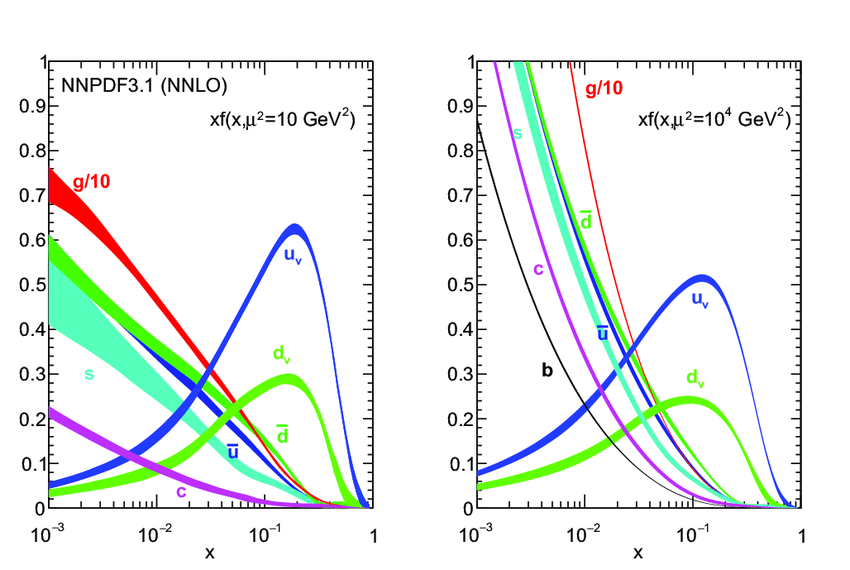
\includegraphics[width=1\textwidth] {figures/Theory/PDF.png}\hspace{1cm}
    \caption{ Parton distribution functions $xf_{q}(x,Q^2)$ for reference momentum transfer $Q^2_{0} = 10 ~ GeV^2$ (left) and $Q^2_{0} = 10^4~ GeV^{2}$ (right)\cite{PDFFigure}.}
\label{fig:PDFFig}
\end{figure}

Any particles with a color charge involved in the interaction or produced during the hard scattering radiate gluons, which further emit QCD radiation forming showers of color particles, also known as \textit{parton shower}. During parton showering, the energy of each parton is split among the radiated particles. Below an energy scale named pole of the QCD running coupling ($\lambda_{QCD}$), the bounding potential of the strong force intervenes, and the partons are bound into a colorless state of stable and unstable hadrons. This process is named \textit{hadronization} and leads to the formation of collimated sprays of charged and neutral hadrons in the detector called \textit{jets}. The matrix element generating the hard-scattering process can describe a few hard QCD emissions. However, dedicated parton showering algorithms are used to describe multiple QCD emissions. The parton shower represents an approximate perturbative treatment of higher-order QCD corrections. The parton showering algorithm calculates dominant contributions associated with soft or collinear parton splitting. The hadronization process is simulated using non-perturbative models. There are two phenomenological models for hadronization, string and cluster models. String models are based on the assumption
that the potential energy between two quarks increases linearly as their spatial separation increases. The cluster model is motivated by considering central objects, hadrons, as a color-neutral cluster of quarks.

The theoretical predictions of an event shown in Figure \ref{fig:ColliderPheno} are calculated using Monte Carlo (MC) simulations which include matrix element calculations for hard scattering, the parton showering, the effect of the underlying events, hadronizations, and pile-up. A comprehensive overview of the methods used in MC simulation is discussed in Ref \cite{EventGenerator}.

	\section{ Electroweak Diboson Physics } 
\label{sec:EWKPheno}

In LHC, two types of physics processes, the QCD production at the order $\alpha_{S}^{\geq 2} \alpha_{EWK}^{4}$ and the EWK production at order $\alpha_{EWK}^{\geq6}$ contribute to the production of di-$Z$ bosons in an association of two jets $[ ZZ( \rightarrow 4\ell) jj ]$ \cite{CMSRun2ZZjj}. Figures \ref{fig:ZZjjFeynmanDiag_QCD_qq} and \ref{fig:ZZjjFeynmanDiag_QCD_gg} show the Feynman diagrams at leading order for parton-initiated and gluon loop-initiated QCD $ZZ^*(\rightarrow 4\ell) jj$ process, respectively, whereas Figure \ref{fig:ZZjjFeynmanDiag_EWk} shows the Feynman diagrams at leading order for the EWK production of $ZZ^*(\rightarrow 4\ell) jj$ \cite{PowhegV2ZZjj}. The EWK production consists of two sets of interactions, first, the Vector Boson Scattering processes involving either triple (Figure \ref{fig:ZZjjFeynmanDiag_EWk_a}) or quartic (Figure \ref{fig:ZZjjFeynmanDiag_EWk_b}) self-interactions of the gauge-bosons, and second the diagrams featuring the Higgs bosons (Figure \ref{fig:ZZjjFeynmanDiag_EWk_c} $\&$ \ref{fig:ZZjjFeynmanDiag_EWk_d}). The scattering amplitudes of the VBS processes involving longitudinally polarized vector bosons grow quadratically with the center of mass energy ($\sqrt{s}$), eventually violating the unitarity bounds. The precise SM interference between the Higgs-featured and VBS processes restores the unitarity \cite{VBSWWWW}.

As discussed in Section \ref{subsubsec:HiggsMech}, the massive $W$ and $Z$ bosons get their masses via the BEH mechanism through EWSB. As a consequence of EWSB, the $W$ and $Z$ bosons acquire an additional degree of freedom (the longitudinal polarization mode) whose scattering interfere with the Higgs-featured processes. Thus, measuring the cross-sections of electroweak production of the di-$Z$ bosons in association with two jets provides a direct probe of the EWSB, which is at the heart of the SM \cite{CMSRun2ZZjj}. As the unitarity is restored at high energies, the cross-section of the electroweak $ZZ^*(\rightarrow 4\ell) jj$ process is sensitive to possible BSM deviations at high energies. Therefore, measuring the cross-sections of the electroweak $ZZ^*(\rightarrow 4\ell) jj$ processes differentially as a function of kinematically sensitive observables is essential. 

\begin{figure}[!htbp]
  \begin{center}
  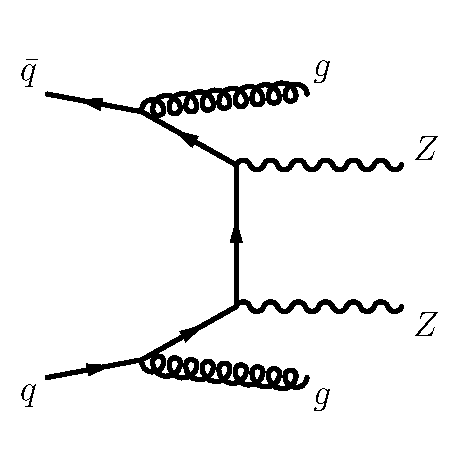
\includegraphics[width=0.31\textwidth]{figures/Theory/diagramQCDZZjjqq.pdf}
  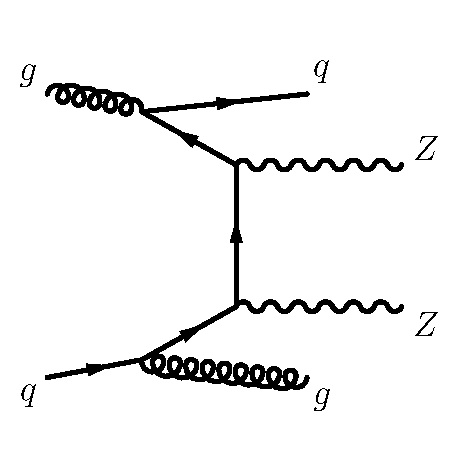
\includegraphics[width=0.31\textwidth]{figures/Theory/diagramQCDZZjjqg.pdf}
  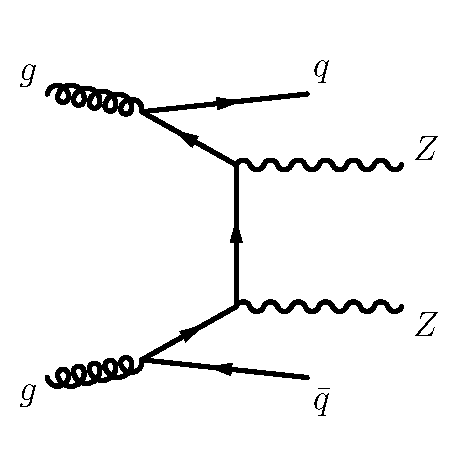
\includegraphics[width=0.31\textwidth]{figures/Theory/diagramQCDZZjjgg.pdf}
   \end{center}
  \caption{Typical diagrams of LO $qq$ and $gg$ induced QCD $\alpha_{S}^2 \alpha_{EWK}^{2}$ production of $ZZ^*jj$. The two $Z\rightarrow \ell \ell$ vertices each contribute an additional electroweak coupling of $\alpha_{EWK}$. \label{fig:ZZjjFeynmanDiag_QCD_qq}}
 \end{figure} 
 
\begin{figure}[!htbp]
  \begin{center}
  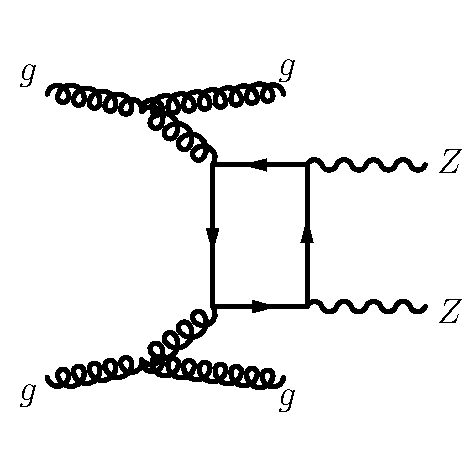
\includegraphics[width=0.31\textwidth]{figures/Theory/diagramQCDZZjjbox.pdf}
  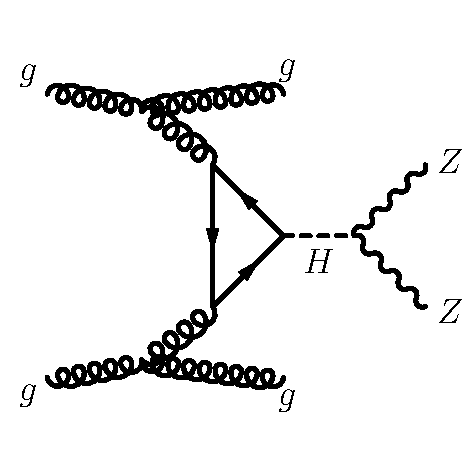
\includegraphics[width=0.31\textwidth]{figures/Theory/diagramQCDZZjjggH.pdf}\\
  \end{center}
  \caption{Typical diagrams for LO $gg$ loop induced the QCD $\alpha_{S}^4\alpha_{EWK}^{2}$ production of $ZZ^*jj$. The two $Z\rightarrow \ell \ell$ vertices each contribute an additional electroweak coupling of $\alpha_{EWK}$. \label{fig:ZZjjFeynmanDiag_QCD_gg}}
 \end{figure}
 
\begin{figure}[!htb]
\begin{subfigure}{.48\textwidth}
  \centering
  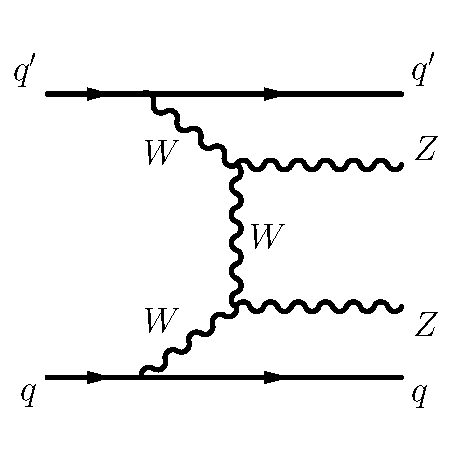
\includegraphics[width=.8\linewidth]{figures/Theory/diagramEWZZjjTGC.pdf}  
  \caption{ZZjj production with two triple gauge coupling (TGC) vertices.}
  \label{fig:ZZjjFeynmanDiag_EWk_a}
\end{subfigure}
\begin{subfigure}{.48\textwidth}
  \centering
  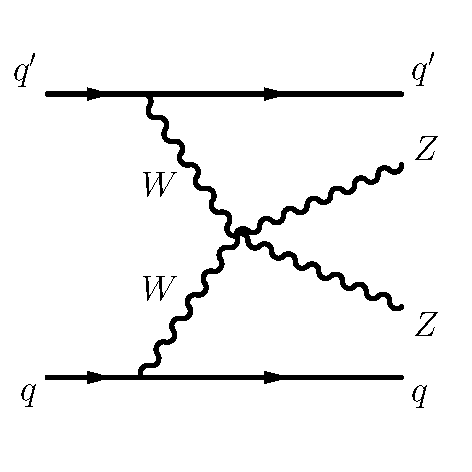
\includegraphics[width=.8\linewidth]{figures/Theory/diagramEWZZjjQGC.pdf}  \\
  \caption{ZZjj production with a quartic gauge coupling (QGC) vertex.}
  \label{fig:ZZjjFeynmanDiag_EWk_b}
\end{subfigure}
\begin{subfigure}{.48\textwidth}
  \centering
  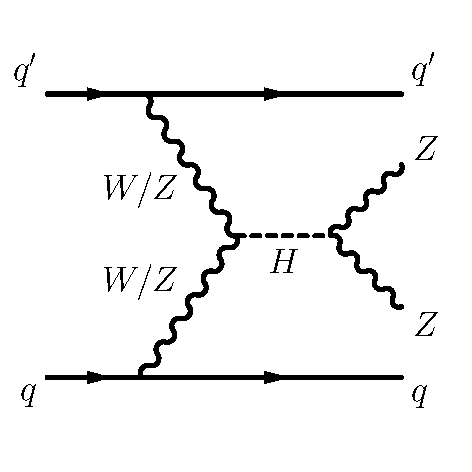
\includegraphics[width=.8\linewidth]{figures/Theory/diagramEWZZjjSchnHiggs.pdf}  
  \caption{s-channel Higgs ZZjj Production.}
  \label{fig:ZZjjFeynmanDiag_EWk_c}
\end{subfigure}
\begin{subfigure}{.48\textwidth}
  \centering
  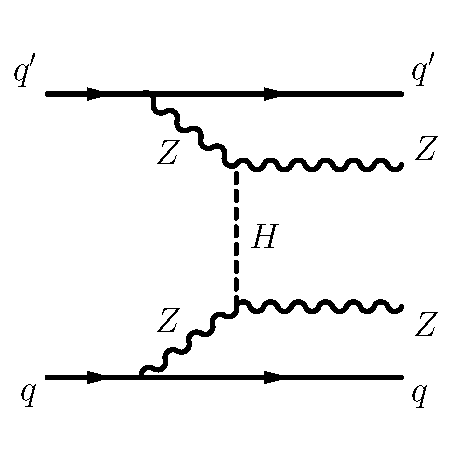
\includegraphics[width=.8\linewidth]{figures/Theory/diagramEWZZjjTchnHiggs.pdf}  
  \caption{t-channel Higgs ZZjj Production.}
  \label{fig:ZZjjFeynmanDiag_EWk_d}
\end{subfigure}\\
\caption{Feynman diagrams at LO for the EWK $\alpha_{EWK}^4$ production of $ZZ^*jj$. The two $Z\rightarrow \ell \ell$ vertices each contribute an additional electroweak coupling of $\alpha_{EWK}$. }
\label{fig:ZZjjFeynmanDiag_EWk}
\end{figure}

The triple and quartic self-interactions of the gauge bosons arise from the square of the non-Abelian structure of $SU(2)$ in the kinetic term $ \frac{1}{4} W^{a}_{\mu\nu} W^{\mu\nu}_{a}$ of the EWK Lagrangian in Equation \ref{eqn:EWKLagrangian1}. Implementing the values of the field strength tensor $W^{a}_{\mu\nu}$ from Equation \ref{eqn:SU2FST}, the relations of $W_{\mu}^{\pm}$ fields in Equation \ref{eqn:RealWBosons}, and the relations of neutral gauge fields in Equation \ref{eqn:NeutralGaugeBosons}, the triple and quartic self interaction terms become, 
\begin{equation}
\mathcal{L}_{3} = ie_{V=\gamma,Z} [ W^{+}_{\mu\nu} W^{-\mu} V^{\nu} - W^{-}_{\mu\nu} W^{+\mu} V^{\nu} + W_{\mu}^{+}W_{\nu}^{-}V^{\mu\nu} ], 
\label{eqn:L_TGC}
\end{equation}
\begin{equation}
\begin{array}{l}
\mathcal{L}_{4} = e^{2}_{W} [ W^{-}_{\mu}W^{+\mu}W^{-}_{\nu}W^{+\nu} - W^{-}_{\mu}W^{-\mu}W^{+}_{\nu}W^{+\nu} ] \\
 \hspace{10pt} + e^2_{V=\gamma,Z} [ W^{-}_{\mu}W^{+\mu}V_{\nu}V^{\nu} - W^{-}_{\mu}V^{\mu}W^{+}_{\nu}Z^{\nu} ] \\
  \hspace{10pt} + e_{\gamma}e_{Z} [ 2W^{-}_{\mu} W^{+\mu} Z_{\nu}A^{\nu} - W_{\mu}^{-}Z^{\mu}W^{+}_{\nu}A^{\nu} - W_{\mu}^{-}A^{\mu}W^{+}_{\nu}Z^{\nu} ],
\end{array}
\label{eqn:L_QGC}
\end{equation}
where $e_{\gamma} = g\sin\theta_{W}$; $e_{W} = \frac{e_{\gamma}}{2\sqrt{2}\sin\theta_{W}}$ $\&$ $e_{Z} = e_{\gamma}\cot\theta_{W}$ are the precise coupling strengths for vector boson self-interaction. Both triple and quartic neutral couplings, such as $ZZZ$ or $ZZZZ$ are absent in the SM. 

Similarly, the couplings of Higgs to vector bosons are also predicted precisely by the BEH mechanism in Equation \ref{eqn:LagBEHKin} as:
\begin{equation}
\mathcal{L}_{HVV} = \frac{m_{W}^2}{v^2} W^{+}_{\mu}W^{-\mu}h^{2} + \frac{m_{Z}^{2}}{v^2} Z_{\mu}Z^{\mu}h^{2}.
\label{eqn:HVVCoupling}
\end{equation}

The EWK production of $ZZ^*(\rightarrow 4\ell ) jj$ is extremely sensitive to any possible anomalous triple gauge couplings (aTGC), anomalous quartic gauge couplings (aQGC), or anomalous Higgs to vector boson coupling \cite{SensitivityNP} \cite{EFT_Eboli} \cite{BSM_Simple2HDM}. Therefore, it is imperative to probe the high energy behavior of the EWK production of $ZZ^*(\rightarrow 4\ell ) jj$ to seek possible deviations from the physics processes beyond the Standard Model (BSM). 

The EWK $ZZ^*(\rightarrow 4\ell ) jj$ production with each $Z$ boson decaying to a pair of SF-OC lepton pair is an extremely rare process. Moreover, with limited statistics in Run$-2$, the QCD background processes dominate the $ZZ^*(\rightarrow 4\ell ) jj$ final state \cite{ATLASZZjj}. Therefore, the differential cross-sections discussed in this thesis are measured in a VBS-Enhanced phase space with a high fraction of events resulting from the EWK $ZZ^*(\rightarrow 4\ell ) jj$ process. The enhanced phase space relies on the characteristic feature of the EWK process with two jets (jj) in the forward-backward region originating from the scattered initial-state quarks. These jets have significant rapidity separation, large invariant mass, and no additional hadronic activity from the hard scattering between the two jets \cite{RapidityGapCite}. The decay of the two Z bosons into SF-OC muons or electron pairs defines the final signature of the VBS-$ZZ^*(\rightarrow 4\ell ) jj$-like event.

\clearpage

\part{Experimental Setup}
\label{sec:Experiment}

The European Organization for Nuclear Research, CERN, in Geneva, Switzerland, is home to the world's largest particle accelerator, the Large Hadron Collider. The measurements presented in this thesis correspond to the processes at the frontier of high-energy collisions. The collisions at the relevant high-energy scale are only possible through large particle accelerators, which reduces the energy loss through synchrotron radiation. The LHC detectors are large in size to effectively measure and stop the high energy particles from collisions. There are currently eight experiments analyzing the data from the LHC, among which ATLAS and CMS are the two largest multipurpose experiments. They analyze the collected data to perform SM precision measurements and direct searches for new physics. This thesis analyzes data collected by the ATLAS experiment between 2015-2018.

This chapter gives a description of the LHC in Section \ref{sec:LHC}, the ATLAS experiment in Section \ref{sec:ATLAS}, details on physics object reconstruction in Section \ref{sec:ParticleReconstruction}, and plans for future upgrades in Section \ref{sec:FutureUpgrades}. 
	\part {\LARGE{The Large Hadron Collider}}
\label{sec:LHC}

\section{ATLAS Detector}
\label{sec:ATLAS}
\section{ATLAS Detector}
\label{sec:ATLAS}

A Toroidal LHC ApparatuS (ATLAS) is a general-purpose detector of LHC that detects events from proton-proton and heavy ion collisions \cite{ATLAS}. It is a $44$ meters long, and $25$ meters wide cylindrical-shaped detector built around LHC Interaction Point 1 \cite{ATLAS}. ATLAS has multiple concentric sub-detectors layered around the beamline, providing forward-backward symmetric coverage. The two proton beams collide at the center of the detector producing outgoing particles from hard scattering, underlying events, and pile-up. The outgoing particles interact with the detector material leaving tracks and energy deposits in several layers of the sub-detectors. The sub-detector closest to the beamline is called \textit{Inner Detector (ID)}, which measures the trajectories of the charged particle and plays a crucial role in identifying the physical position of hard-scattering, also known as the \textit{interaction point (IP)}. ID is surrounded by a solenoid magnet that provides a $2$ T magnetic field to bend the particle trajectories for momentum measurements \cite{ATLAS}. After the solenoid magnet lies the \textit{electromagnetic calorimeter (ECAL)} and then the \textit{hadronic calorimeter (HCAL)}, which measure the energy of electromagnetic and hadronic physic objects, respectively. The outermost layer of the ATLAS detector is the \textit{Muon Spectrometer(MS)} that provides a secondary measure of muon trajectories for momentum measurement. MS is embedded inside a toroidal magnetic field that provides a magnetic field up to 3.5 T \cite{ATLAS}. Figure \ref{fig:ATLAS} shows a schematic of the ATLAS detector with all its sub-detectors.

\begin{figure}
    \centering
    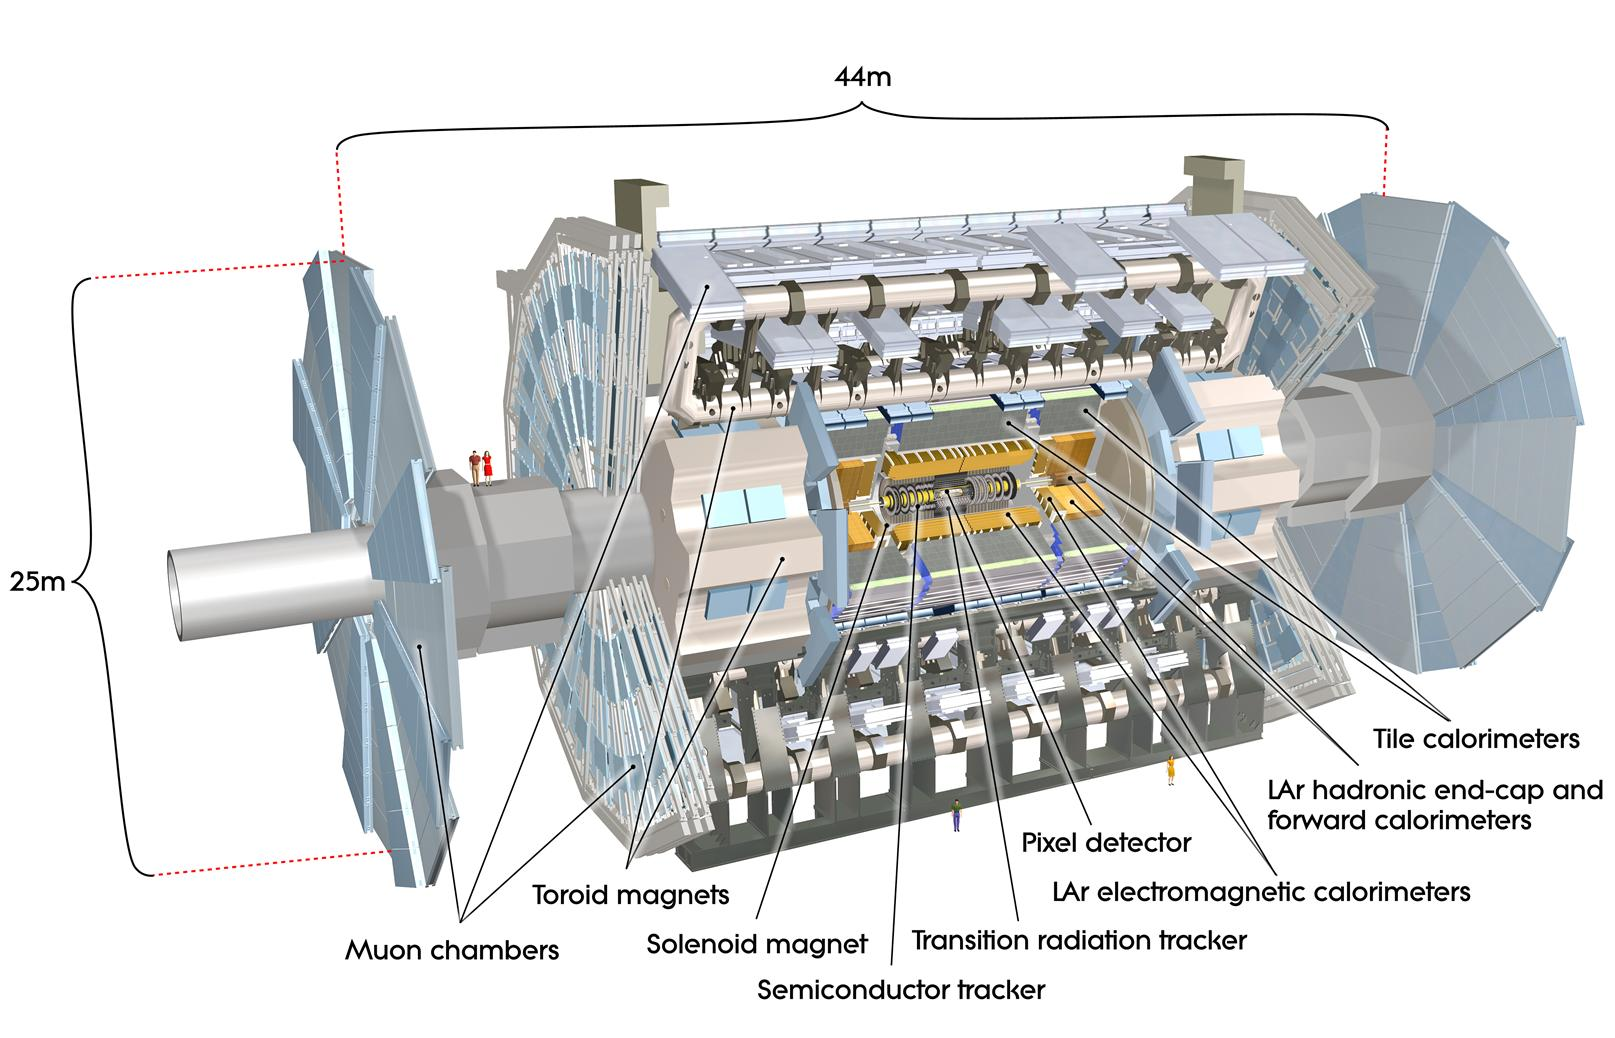
\includegraphics[width=.98\linewidth]{figures/LHC/AtlasDetector.png}
    \caption{ A detailed schematic of the ATLAS detector with all its sub-detectors \cite{ATLAS}.\label{fig:ATLAS}}
\end{figure}

\subsection{ATLAS Coordinate System}
\label{subsec:ATLASCS}

ATLAS measurements use a right-handed coordinate system with the nominal interaction point as the origin. The beamline is along the cylindrical symmetry axis of the detector, which defines the longitudinal \textit{z}-axis. The transverse \textit{xy}-plane is perpendicular to the beam direction, where \textit{x}-axis points to the center of the LHC ring and \textit{y}-axis points upwards towards the surface. Figure \ref{fig:ATLAS_CS} shows a schematic of the ATLAS coordinate system. The angle measured around the beamline in \textit{xy}-plane gives the azimuthal angle $\phi$, whereas the angle measured with respect to the \textit{z}-axis gives the polar angle $\theta$. Transverse momentum ($p_{T}$) is particle's momentum in the \textit{xy}-plane, defined as, 

\begin{equation}
p_{T} = \sqrt{p_{x}^2+p_{y}^2}=p\sin\theta
\label{eqn:pT}
\end{equation}
\textit{Rapidity (y)} defined in terms of a particle's energy ($E$) and momentum ($p$) is a commonly used collider physics quantity that measures whether an outgoing particle is produced perpendicular or parallel to the \textit{z}-axis. Rapidity is defined as, 

\begin{equation}
    y = \frac{1}{2}\ln{ \left( \frac{E+p_{z}}{E-p_{z}} \right) }
    \label{eqn:Rapidity}
\end{equation}
Particles with larger momentum along the \textit{z}-axis have larger values of rapidity, whereas particles with larger momentum values in the transverse plane have smaller values of rapidity. For particles with negligible mass, the rapidity approaches a purely angular variable called \textit{pseudorapidity ($\eta$)} defined as, 

\begin{equation}
    \eta = \frac{1}{2}\ln{ \left( \frac{ |\vec{p}|+p_{z}}{ |\vec{p}| -p_{z}} \right) } = -ln { \left[ \tan \left( \frac{\theta}{2}\right) \right] } 
    \label{eqn:PseudoRapidity}
\end{equation}
Higher values of rapidity and pseudorapidity refer to the forward region of the detector. ATLAS detector has full $2\pi$ coverage in $\phi$ and maximum coverage up to $|\eta| < 4.5$ corresponding to $1.3^{\circ} < \theta < 178.7^{\circ} $ \cite{ATLAS}. 

\begin{figure}
    \centering
    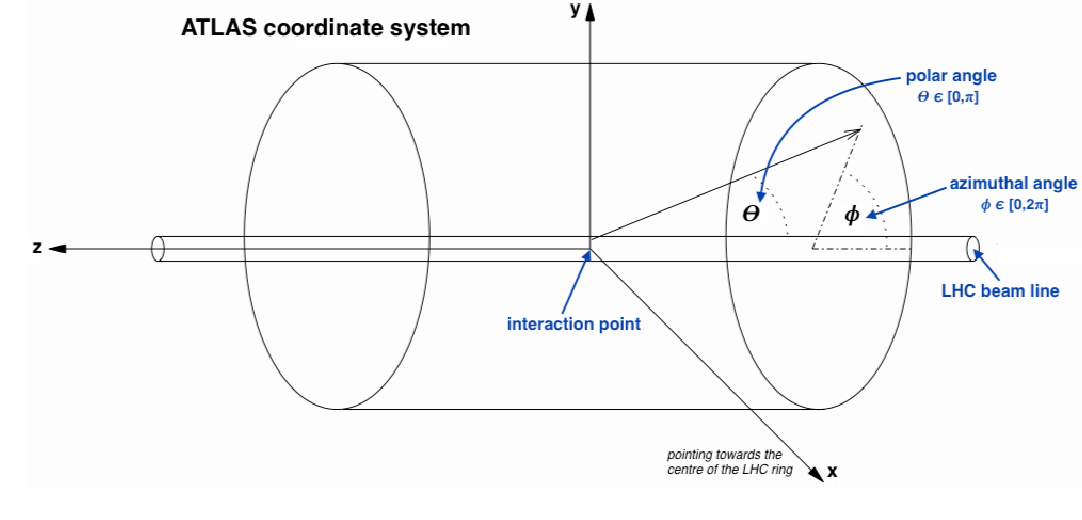
\includegraphics[width=.98\linewidth]{figures/LHC/ATLAS_CoordinateSys.png}
    \caption{ A schematic of the right-handed ATLAS coordinate system \cite{ATLAS_CoordSys}.\label{fig:ATLAS_CS}}
\end{figure}

\subsection{Inner Detector}
\label{subsec:ID}
The inner detector is the innermost sub-detector of ATLAS and is responsible for tracking charged particles' trajectories and identifying the interaction point of the hard scatter. Closest to the interaction point is the Insertable B-Layer (IBL) \cite{ATLAS_IBL}, which was installed during the long-upgrade shutdown between Run-1 and Run-2 to meet the requirements for competent tracking at higher pile-up. The IBL is highly granular, consisting of roughly 12 million silicon pixel sensors with a size of $50\times 250 ~\mu m^2$ \cite{ATLAS_IBL}. IBL is located $3.3$ cm from the beamline and can reconstruct tracks within the pseudorapidity range of $|\eta|<2.5$ \cite{ATLAS_IBL}. 

Three layers of silicon-pixel detectors with $1,744$ pixel sensors, each comprising $47,232$ pixels of size $50\times 400 ~\mu m^2$ surround the IBL \cite{ID_Pixel}. The slightly larger pixel size is adequate for the pile-up at a distance larger than $5$ cm from the interaction point. These pixel layers were also present during the Run-1 data-taking period and provided coverage up to $|\eta|<2.5$ with a spatial resolution of tracks between $5$ and 12 $\mu$m \cite{ID_Pixel}. Surrounding the pixel layers is the Semiconductor Tracker (SCT) consisting of five layers of silicon microstrip detectors with a mean strip pitch of $80 ~\mu m$ in the barrel region and varying pitch of  $57-94 ~\mu m$ in the end-cap regions \cite{ID_Strips}. 

At a distance about $50$ cm from the beamline lies the outermost layer of the ATLAS inner detector, the Transition Radiation Tracker (TRT), with $370,000$ straw tubes with a diameter of $4$ mm \cite{ID_TRT}. Each TRT straw tube is filled with a Xenon-based gas mixture and consists of $31~\mu m$ diameter tungsten wires \cite{ID_TRT}. A charged particle passing through different layers of ID leaves a track via ionization. 

Figure \ref{fig:ATLAS_ID} schematically shows different parts of the inner detector and their distances from the interaction point.

\begin{figure}
    \centering
    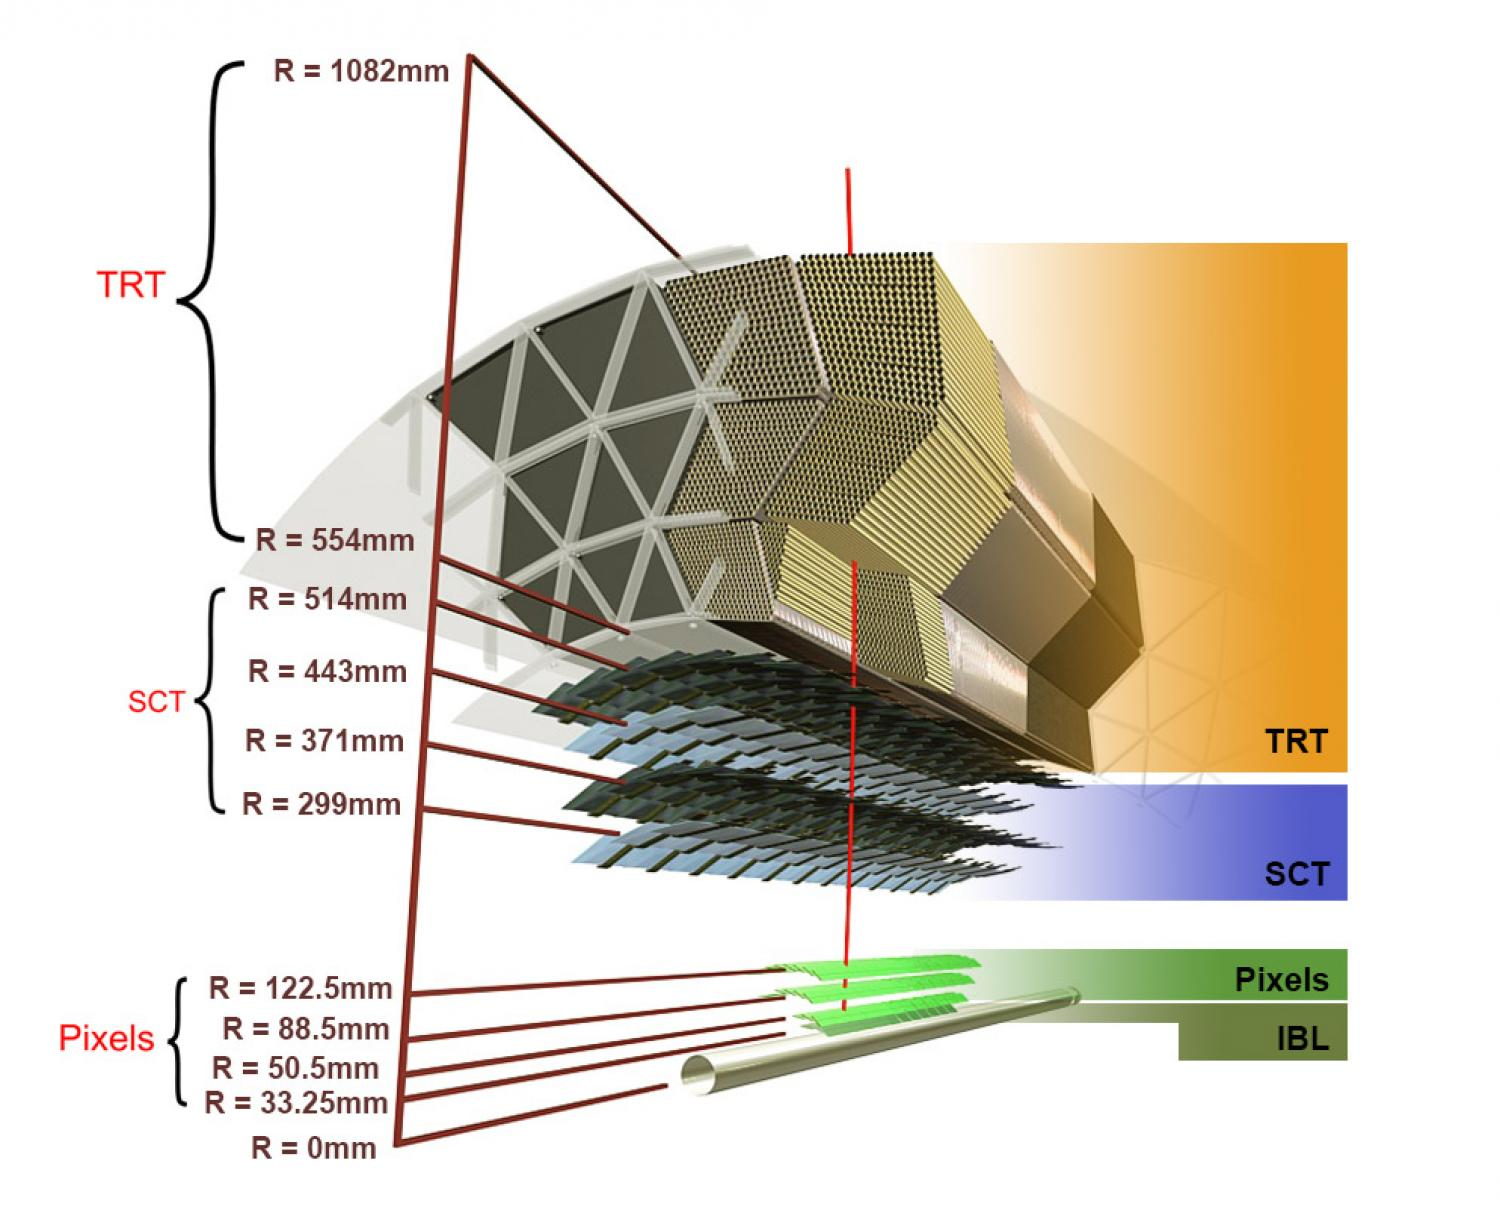
\includegraphics[width=.98\linewidth]{figures/LHC/ATLAS_InnerDetector.jpg}
    \caption{ A schematic of the inner detector of ATLAS showing the IBL, pixel detectors, SCT, and TRT \cite{ID_Align_Run2}.\label{fig:ATLAS_ID}}
\end{figure}

\subsection{Calorimeters}
\label{subsec:Cal}

ATLAS has two calorimeters, electromagnetic and hadronic, designed to measure the energy of charged and neutral particles up to the range of $|\eta|\leq4.9$ \cite{ATLAS}. When interacting with a material, an electron loses its energy by photon emission, which could produce a pair of $e^{+}e^{-}$ and vice versa, creating an electromagnetic shower in the detector. Similarly, the hadronic particles also result in a shower of particles through multiple scattering. The calorimeters measure the energy of the particles by reconstructing the electromagnetic and hadronic showers. The calorimeters are designed to capture all particles except muons and neutrinos. Therefore, motivated by the need to prevent \textit{punch-through}\footnote{particles' probabilities of passing through the calorimeters} effect, materials with high radiation length ($X_{0}$) and high interaction length ($\lambda$) are chosen to construct the calorimeters.

Outside the solenoid magnet surrounding the ID is the accordion-shaped electromagnetic calorimeter consisting of an alternate layer of lead absorber plates and highly granular liquid-argon (LAr) cells to precisely measure the energies of electrons and photons. It comprise of barrel section in $|\eta| < 1.475$ range and two end-caps in $1.375 < |\eta| < 3.2$ range \cite{ATLAS_ECAL}. The calorimeter's central region ($|\eta| < 2.5$) is designed to identify electrons and photons with high precision.

The hadronic calorimeter surrounds the ECAL and consists of a steel absorber and active scintillator tiles in the $|\eta| < 1.7$ range. In the end-caps range of $1.5 < |\eta| < 3.2$, it consists of a copper absorber and active LAr detectors. The forward region ranging from $3.2 < |\eta| < 4$ comprises the tungsten absorber followed by active LAr detectors \cite{ATLAS_HCAL}. 

Figure \ref{fig:ATLAS_Cals} schematically shows the layout of ATLAS calorimeters. 

\begin{figure}
    \centering
    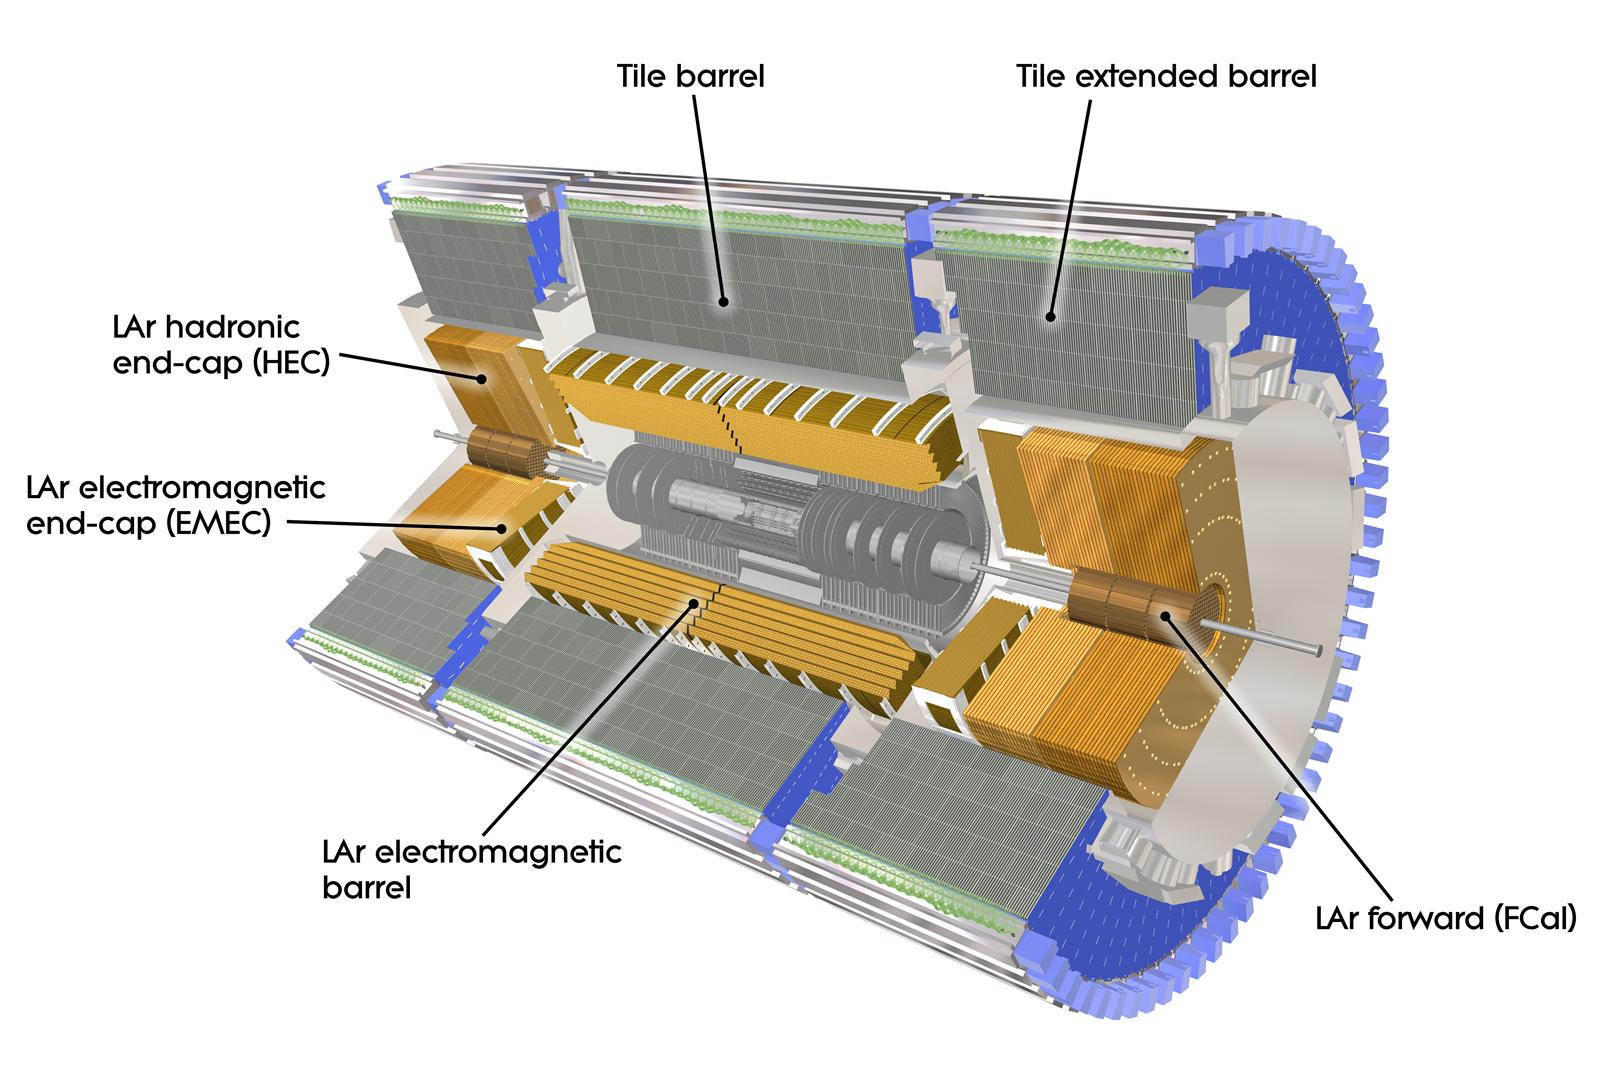
\includegraphics[width=.98\linewidth]{figures/LHC/ATLAS_CALO.jpeg}
    \caption{ A schematic of electromagnetic and hadronic calorimeters In ATLAS \cite{ATLAS}.\label{fig:ATLAS_Cals}}
\end{figure}

\subsection{Muon Spectrometer}
\label{subsec:MS}
In ATLAS, muons are deeply-penetrating charged particles that leave minimum ionizing deposits in the calorimeter. The muon spectrometer, the outermost part of the ATLAS detector, tracks trajectories of muons deflected in $0.5$ magnetic field provided by the superconducting toroidal magnets, giving an additional measure of muon's momentum \cite{ATLAS}. The MS tracks muon with $p_{T} > 3$ GeV in $|\eta| < 2.7$ range \cite{ATLAS}. As shown in figure \ref{fig:ATLAS_MS}, the muon spectrometer comprises four types of detectors; first, the three stations of Monitored Drift Tubes (MDT) in $|\eta| < 2.0$ region followed by the Cathode Strip Chambers (CSC) in  $2.0 < |\eta| < 2.7$ region \cite{ATLAS}. The other two detectors are the Resistive Plate Chambers (RPC) in $|\eta| < 1.05$ and the Thin-gap Chambers (TGC) beyond $|\eta| = 1.05$ comprising the trigger system in MS \cite{ATLAS}. 

\begin{figure}
    \centering
    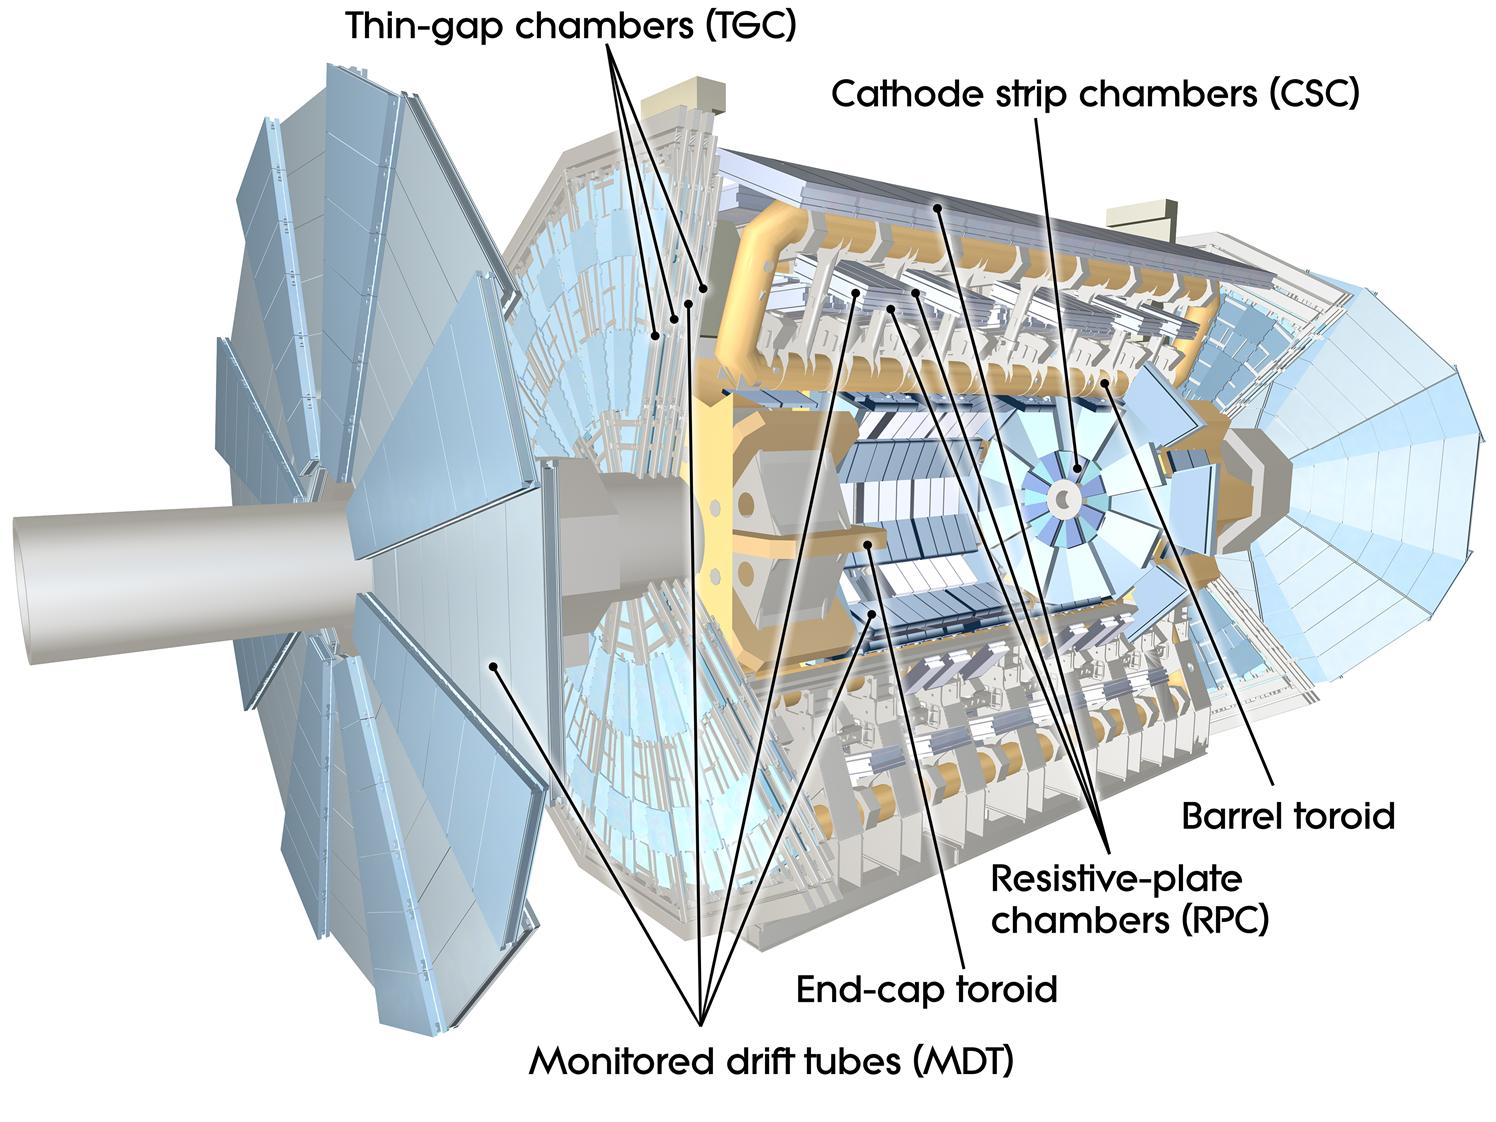
\includegraphics[width=.98\linewidth]{figures/LHC/ATLAS_MS.jpeg}
    \caption{ A schematic of different components of the muon spectrometer in ATLAS \cite{ATLAS}.\label{fig:ATLAS_MS}}
\end{figure}

\section{ Physics Object Reconstruction} 
\label{sec:ParticleReconstruction}
\section{ Physics Object Reconstruction} 
\label{sec:ParticleReconstruction}
Different particles leave unique signatures in different sub-detectors of ATLAS. Figure \ref{fig:ATLASTransverse} shows a schematic of simplified representation of various particles passing through different sub-detectors and leaving various signature. Physics object reconstruction is the process of interpreting these signals to meaningful information about the outgoing particles. This section discusses the detail of reconstruction relevant to the thesis. 

\begin{figure}
    \centering
    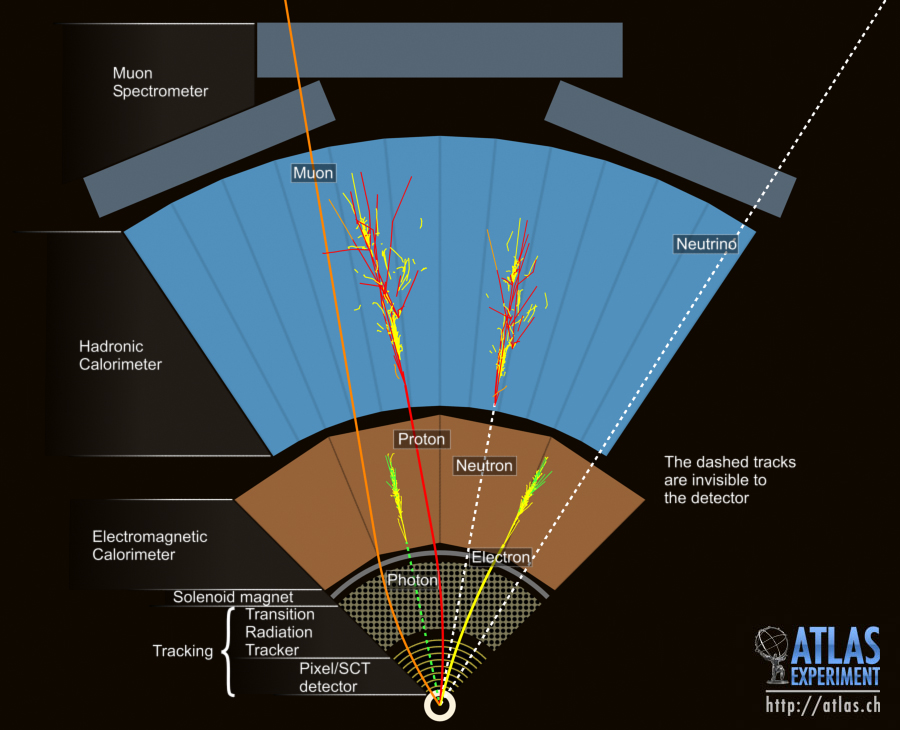
\includegraphics[width=.98\linewidth]{figures/LHC/ATLAS_Transverse.jpg}
    \caption{ Simplified representation of various particles traversing through different layers of ATLAS sub-detectors and leaving unique signatures \cite{ATLASTransverse}.\label{fig:ATLASTransverse}}
\end{figure}

\subsection{Trigger}
\label{subsec:TriggerATLAS}
The first step of particle and event reconstruction is selecting interesting high-energy events from a pool of lower-energy multiple-scattering signals. The high bunch crossing frequency of every $25$ ns results from a large amount of data making it physically impossible to store all events. ATLAS trigger system selects the events interesting for physics objects. 

ATLAS trigger consists of two levels, Level 1 (L1) trigger integrated into the hardware and high-level software trigger (HLT) \cite{TriggerSystemATLAS}. The L1 trigger is based on custom-built electronics, which uses signals from the calorimeters and muon trigger system (TGC and RPC) to identify event features such as electrons, photons, jets, taus, and missing energy. The L1 trigger reduces the $40$ MHz incoming collision data-rate corresponding to $25$ ns bunch crossing by a factor of $400$ to $100$ kHz output \cite{TriggerSystemATLAS}. The events accepted by the L1 trigger defines regions of interest (ROI), and HLT algorithms are run on these events to select ones with candidate physics objects and kinematic requirement. The software-based HLT trigger further reduces the data rate by almost a factor of 100 to $1.5$ kHz \cite{ATLAS}. With the combination of L1 and HLT trigger system, the data rate is reduced by $400,000$, and the selected events corresponding to data readout of $1.5$ GB are stored in the permanent storage. Figure \ref{fig:DAQ} shows the schematic of ATLAS's trigger and data acquisition system. 

\begin{figure}
    \centering
    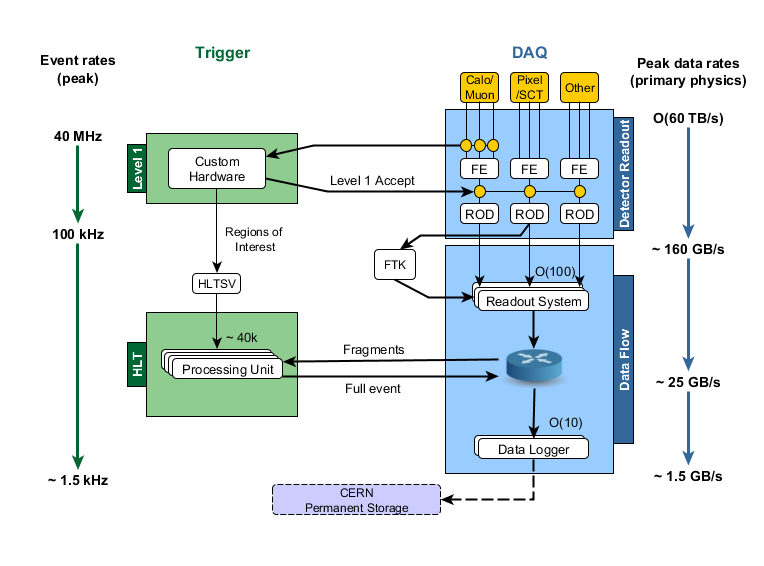
\includegraphics[width=.98\linewidth]{figures/LHC/DAQ_ATLAS.png}
    \caption{ Trigger and data acquisition system in ATLAS \cite{ATLAS_DAQ}.\label{fig:DAQ}}
\end{figure}

Physics object reconstruction discussed below converts the raw data output stored in permanent storage to physics objects used in physics analyses. 

\subsection{Tracks and Vertices Reconstruction}
\label{subsec:Tracking}
Tracking a charged particle is a critical step in reconstruction. The tracks of the charged particles play an essential role in momentum measurement, particle identification, and primary vertex reconstruction through the extrapolation of tracks to the interaction point. As the inner detector is closest to the beamline and comprises minimally ionizing detector material with high granularity, it plays a crucial role in track reconstruction. The ID magnetic field is homogenous, resulting in circular tracks of the charged particles. Five parameters define charged particle tracks; the ratio of charge and transverse momentum ($q/p_{T}$) defining the curvature; the distance of the closest approach to the primary vertex in $xy$-plane defining the transverse impact parameter ($d_{0}$), the longitudinal impact parameter ($z_{0}$) along the $z$-axis; the azimuthal angle ($\phi_{0}$) and the polar angle ($\theta_{0}$) of the particle direction at the closest approach point \cite{TrackingRun2_ATLAS}. Figure \ref{fig:TrackParameter} schematically shows the five-track parameters. 

\begin{figure}
    \centering
    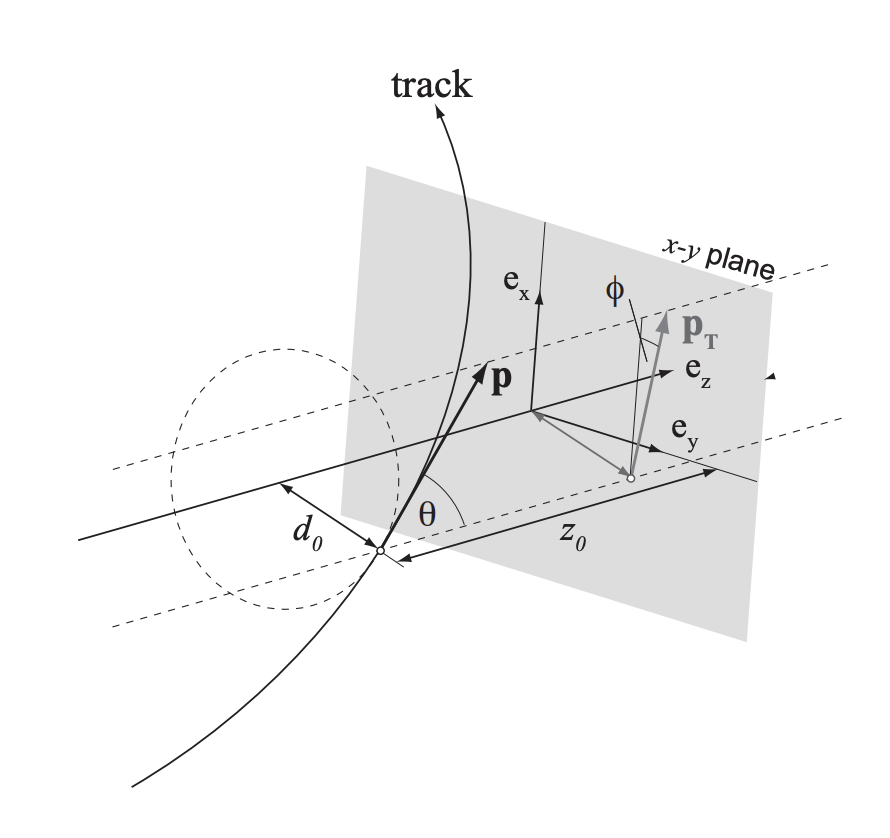
\includegraphics[width=.98\linewidth]{figures/LHC/TrackParameters.png}
    \caption{ Schematic showing the five-track parameters \cite{TrackParameterFig}.\label{fig:TrackParameter}}
\end{figure}

As shown by figure \ref{fig:TrackingOutline}, track reconstruction follows two different approaches used in Run-2; the primary \textit{inside-out} approach and the secondary \textit{outside-in} approach \cite{TrackingRun2_ATLAS}. The first step in the inside-out track reconstruction is the space point and drift circle formation, formed respectively by the clusters of signals from the silicon detectors and drift-circles hits in the TRT. Second, track seeds are formed from a collection of three silicon-detector space points and extrapolated to the outer layers by including the compatible clusters in the track trajectory. Once the track is formed, an ambiguity resolution algorithm is applied to reassign shared clusters to the track with a better match, and the final track candidate is fitted using a global $\chi^{2}$ method. The last step of inside-out track reconstruction is adding compatible TRT drift holes and refitting the tracks. 

\begin{figure}
    \centering
    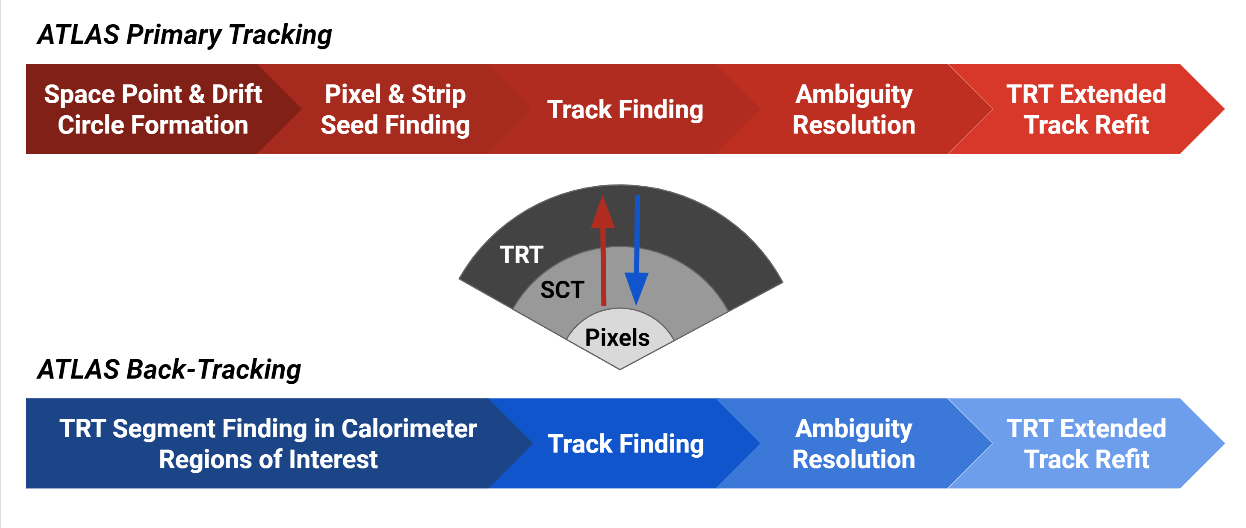
\includegraphics[width=.98\linewidth]{figures/LHC/trackingflowchart.png}
    \caption{schematic showing the two types of track reconstruction, primary inside-out and secondary outside-in. Taken from ATLAS Tracking CP group public tutorial \url{https://atlassoftwaredocs.web.cern.ch/trackingTutorial/idoverview/}. \label{fig:TrackingOutline}}
\end{figure}

The inside-out method is optimal for particles that minimally interact with the inner-detector material. However, secondary backtracking with an outside-in approach is needed for particles interacting with the inner detector, such as reconverted photons. In this approach, the track pattern recognition starts at the TRT in the regions of interest flagged by the electromagnetic calorimeter and backtracks to the silicon detectors. 

Tracks of the charged particle are extrapolated inward to the beamline and are assigned to vertices \cite{VertexReconstruction}. In most ATLAS analyses, including the one presented in this thesis, the space-point with the highest quadrature sum of track $p_T$ ($\sum_{track}{p_{T}^2}$) is identified as the primary vertex of an event.

\subsection{Electron Reconstruction}
\label{subsec:ParticleRecon_Elec}
Electrons, when interacting with a material, produce a photon by bremsstrahlung radiation, the process defining the interaction of a charged particle with the electric field of an atomic nucleus. Any energetic photon, either from a physics process or bremsstrahlung, can turn into a pair of $e^{+}e^{-}$, which can again radiate another set of photons, thus, giving rise to an electromagnetic shower. For given energy and material, electromagnetic showers have a characteristic penetration depth.

ATLAS electrons are reconstructed by combining the tracking information from the ID, and the energy deposits in nearby cells of the calorimeter,  energy clusters \cite{ElectronReco}. The clusters are formed only if the energy deposit exceeds four times the expected deposits from the pile-up. The reconstruction efficiency for high-energy electrons with transverse energy ($E_{T}>15$ GeV) is about $97-99\%$ \cite{ElectronReco}. \textit{Prompt electrons} originate from the hard scattering and are the primary interest of physics analysis. However, the detector has electrons from \textit{non-prompt sources} including the jets, misidentification, and pile-up. Therefore it is imperative to identify and isolate the prompt electrons in an event, and the efficiency for identification and isolation varies as a function of $E_{T}$. Limited by the coverage of the electromagnetic calorimeter, only electrons within the $|\eta| <2.47$ range can be reconstructed and identified as prompt in ATLAS.

The electron identification is based on a multivariate-likelihood (LH) technique which takes information from tracking detectors and calorimeters as input. The tool is trained to separate signal and background probability density functions using simulated $Z \rightarrow ee$ and $Z \rightarrow J / \psi$ events. The LH tool provides four \textit{working points}, VeryLoose, Loose, Medium, and Tight, at different values of the LH discriminant to cover various needs of several ATLAS analyses. The analysis presented in this thesis uses electrons satisfying the Loose identification working point with at least one hit in the IBL. 

Prompt electrons originating from W, Z, or H decay are characterized by low activity around them in the $\eta-\phi$ plane. An isolation requirement is applied to the electron candidates to select ones from the hard scattering. Calorimeter and track-based requirements on isolation variables are defined to quantify the isolation. The variables are based on the amount of activity around an isolation cone of the candidate electron. Calorimeter-based isolation relies on the variable $E_{T,cone}^{iso}$, the sum of transverse energies inside a $\deltaR=0.2$ cone of the electron candidate. Similarly, the track-based isolation variable is $p_{T,cone}^{iso}$, the sum of the transverse momentum of the electron candidate within a $p_{T}-$dependent $\Delta R$, which is defined as, 

\begin{equation}
\Delta R = min \left( \frac{10 GeV}{p_{T}},\Delta R_{max} \right)
\end{equation}

where the maximum cone size is $\Delta R_{max} = 0.2$. Similar to the identification, several working points are available for electron isolation. The measurement in this thesis uses the \textit{Loose$\_$VarRad} isolation working point which requires $E_{T,cone}^{iso} < 0.3$ and $p_{T,cone}^{iso} < 0.15$. Figure \ref{fig:ElecEff} shows the electron identification and isolation efficiencies as a function of their $E_{T}$. The Loose working point has the highest identification and isolation efficiencies and is the optimal working point for the measurement because of the fully reconstructable final state.

\begin{figure}
    \centering
    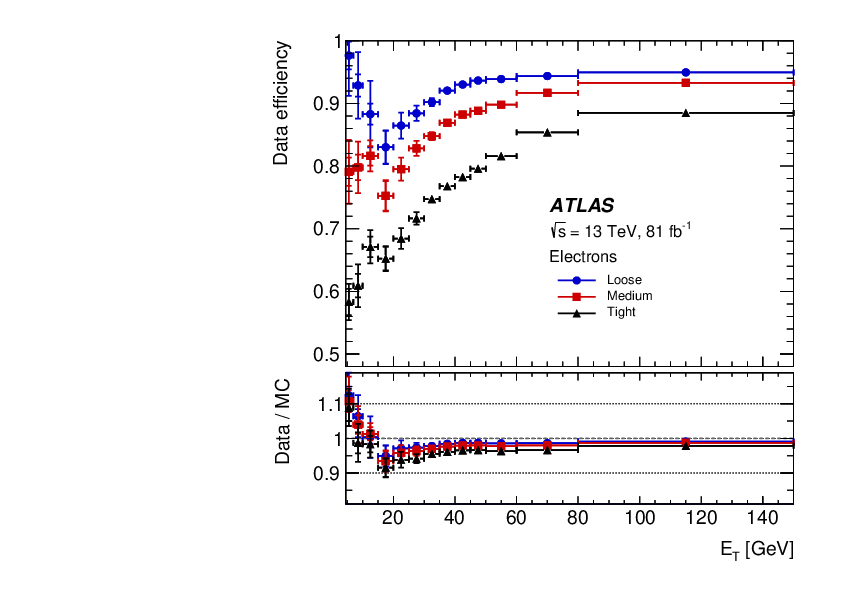
\includegraphics[width=.49\linewidth]{figures/LHC/ElecIdent_Eff.png}
    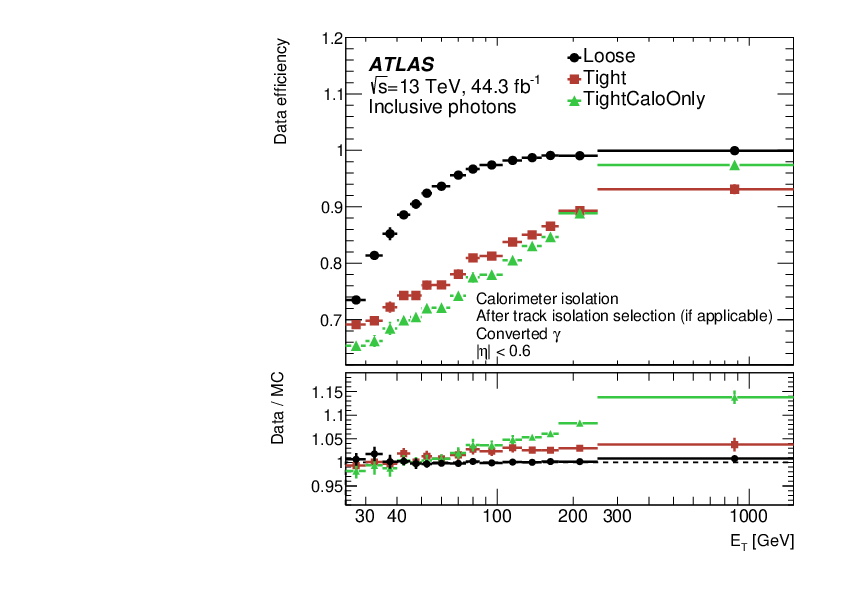
\includegraphics[width=.49\linewidth]{figures/LHC/Elec_IsoEff.png}
    \caption{ Distributions showing the identification (left) and isolation (right) efficiencies for electrons as a function of their $E_{T}$\cite{ElectronReco}.\label{fig:ElecEff}}
\end{figure}

The total electron efficiency is defined as the product of the electron reconstruction, identification, isolation, and trigger efficiencies as, 

\begin{equation}
    \epsilon_{total} = \epsilon_{reco} \times \epsilon_{id} \times \epsilon_{iso} \times \epsilon_{trigger}     
\end{equation}

Each of the efficiency terms is evaluated on data and MC. \textit{Scale Factors (SF)} defined as the ratio of the measured efficiency in data and the efficiency simulated in MC are derived and applied to the simulation to match the one observed in the data. Typically, SFs are close to one, and systematic uncertainties related to scale factors are considered in the measurement.

\subsection{Muon Reconstruction}
\label{subsec:ParticleRecon_Muon}
The rate of bremsstrahlung radiation is inversely proportional to the square of a particle's mass. Since muons are about $200$ times heavier than electrons, they primarily interact with the detector material through ionization. Therefore, muons are minimally ionizing particles that do not create electromagnetic shower in the calorimeters and pass through all layers of the ATLAS detector. Hence, muon detection relies on track measurements from the inner detector and muon spectrometer. As shown in figure \ref{fig:MuonFig}, four types of muons are defined based on the type of sub-detectors used during a muon reconstruction,

\begin{itemize}
    \item{\textbf{Combined muons:} muons reconstructed from a global refit of ID and MS tracks }
    \item{\textbf{Segment-tagged muons:} muons reconstructed from a fitted ID track and MS segment track } 
    \item{\textbf{Calo-tagged muons:}  muons reconstructed using ID track matched to the minimum ionizing energy deposits in the calorimeters}
    \item{\textbf{Standalone Muons:} muons reconstructed solely from the MS tracks }
\end{itemize}

\begin{figure}
    \centering
    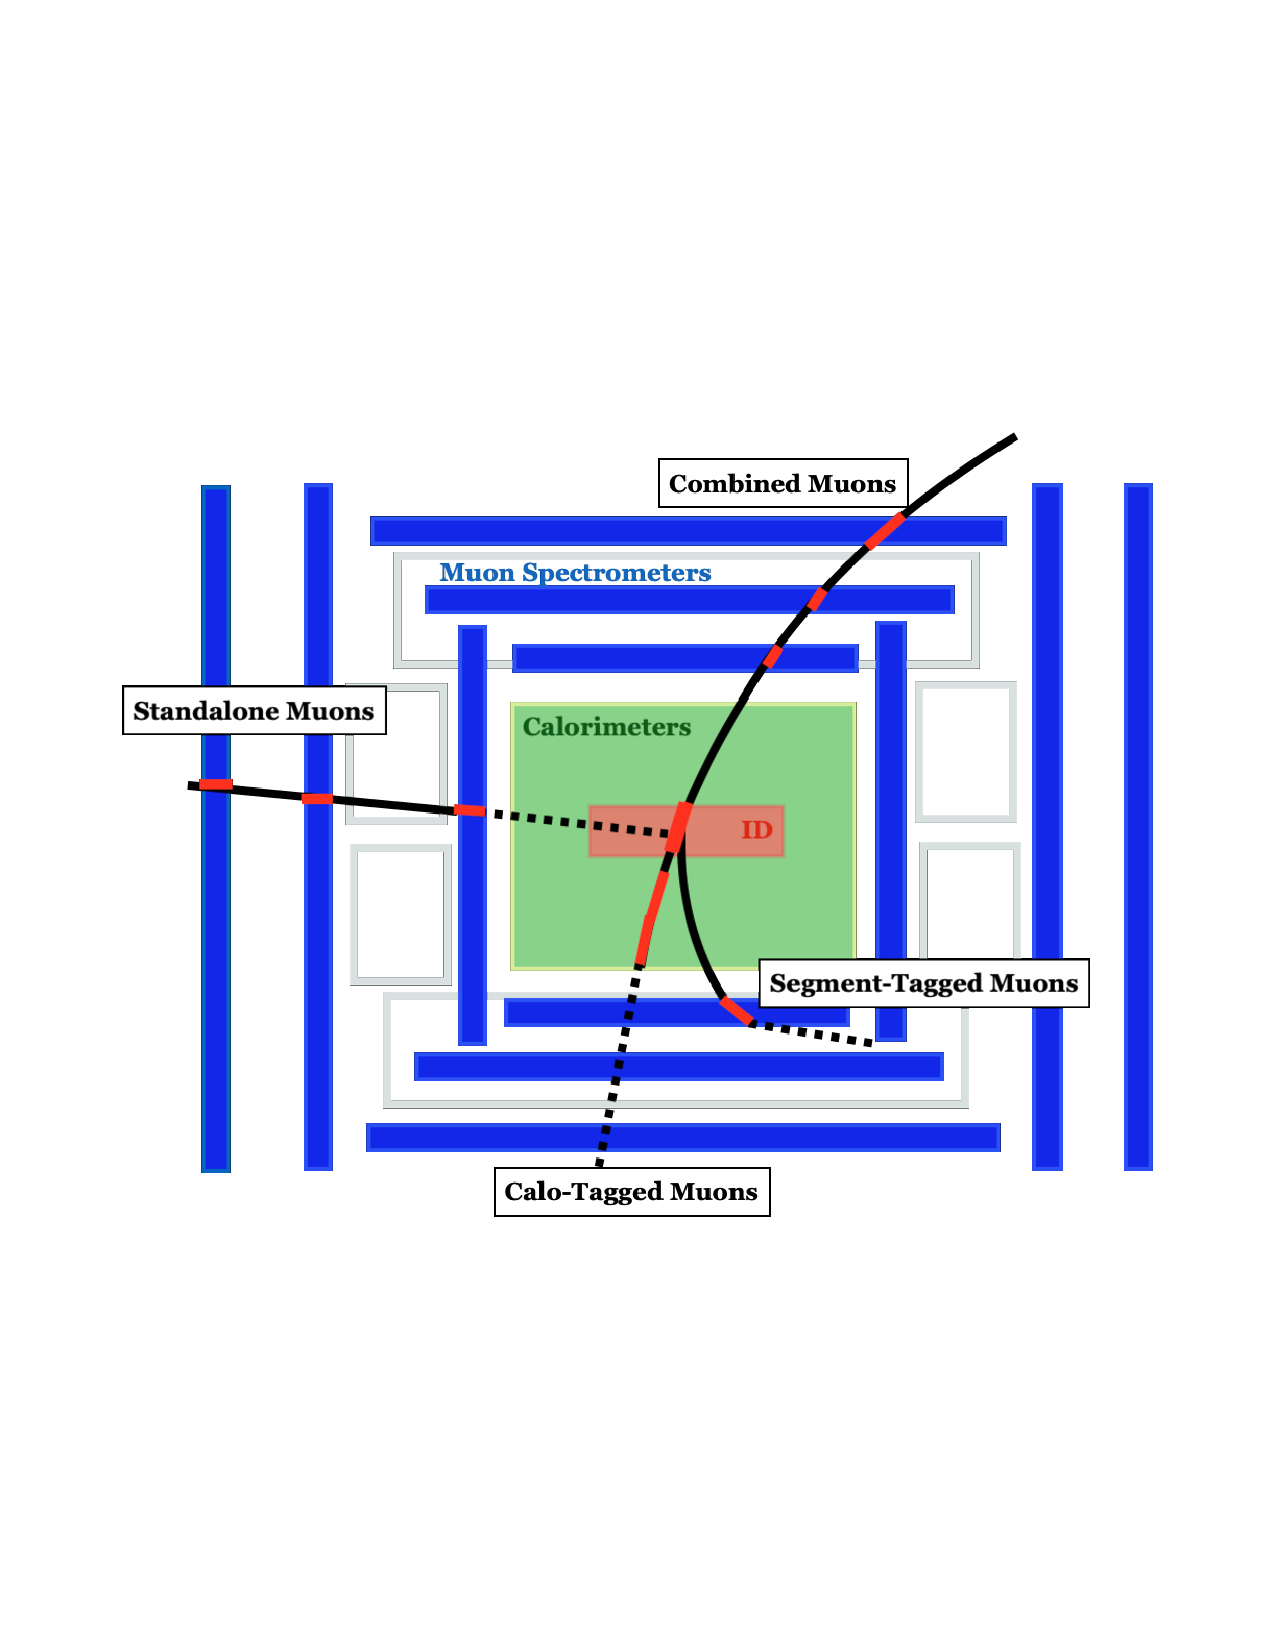
\includegraphics[width=.5\linewidth]{figures/LHC/MuonTypes.pdf}
    \caption{ Schematic of four different types of muons reconstructed using several layers of sub-detectors \cite{MuonReco}.\label{fig:MuonFig}}
\end{figure}

Similar to the electron reconstruction discussed in Section \ref{subsec:ParticleRecon_Elec}, reconstructed muons from the hard scatter are identified and isolated from the muons originating from secondary sources. Muon identification working points are developed by applying quality requirements in the simulated $t\bar{t}$ events where a $W$ from top-quark decay decays to a muon and a neutrino. The quality cuts require at least one-pixel hit, five SCT hits, less than three pixel or SCT holes, and at least $10\%$ of TRT hits to be included in the fit for the $0.1<\eta<0.9$ range with full TRT coverage \cite{MuonReco}. Three variables are used in muon identification; $q/p$ significance, which is defined as the ratio of muon's charge and momentum divided by the sum-quadrature of their uncertainties; $\rho^{'}$ defined as the absolute difference of transverse momentum measurements in the ID and MS divided by the combined track's $p_{T}$; and the normalized $\chi ^{2}$ of the combined track fit \cite{MuonReco}. 
Four identification \textit{working points}, Loose, Medium, Tight, and High-$p_{T}$ are defined for muons. The measurement uses a Loose identification point, which comprises all four types of muons and is developed for processes with four leptons in the final state  \cite{MuonReco}. 

To evaluate the total reconstruction efficiency of muons, $Z \rightarrow \mu\mu$ and $J/\psi \rightarrow \mu\mu$ events are used. The reconstruction efficiency in the region with ID coverage $|\eta|<2.5$ is obtained by using the tag-and-probe method, whereas, for $|\eta|>2.5$ region, it is estimated by evaluating SFs based on a double ratio of data and MC in $Z \rightarrow \mu\mu$ events \cite{MuonEffLargeEta}.

Analogous to electrons, muons are required to meet calo-based and ID-based isolation requirements. Muons in the measurement satisfy \textit{PflowLoose$\_$VarRad} isolation working point. Like in the case of electrons, systematic uncertainties on different scale factors for muon reconstruction, identification, isolation, and trigger efficiencies are propagated to the final cross-section measurement.

\subsection{Jet Reconstruction}
\label{subsec:ParticleRecon_Jets}


\section{Future Upgrades}
\label{sec:FutureUpgrades}
\section{Future Upgrades}
\label{sec:FutureUpgrades}

\subsection{High Luminosity LHC}
\label{subsec:HLLHC}
The planned High Luminosity Large Hadron Collider (HL-LHC) is expected to operate starting mid-2029. The primary goals of HL-LHC are to collect large high-quality data statistics needed to study rare SM processes such as Higgs self-interaction, Higgs couplings to lighter particles, the longitudinal component of vector boson scattering, and to extend the BSM searches beyond the current reach of LHC. The HL-LHC upgrade aims to increase the center-of-mass energy of proton-proton collisions to $\sqrt{s}=14$ TeV and the instantaneous luminosity up to $\mathcal L = 7.5 \times 10^{34} cm^{-2}s^{-1}$ \cite{HLLHC}. Figure \ref{fig:HLLHC} shows the complete operation of LHC starting in 2011 to the planned decade-long HL-LHC program. 

\begin{figure}
    \centering
    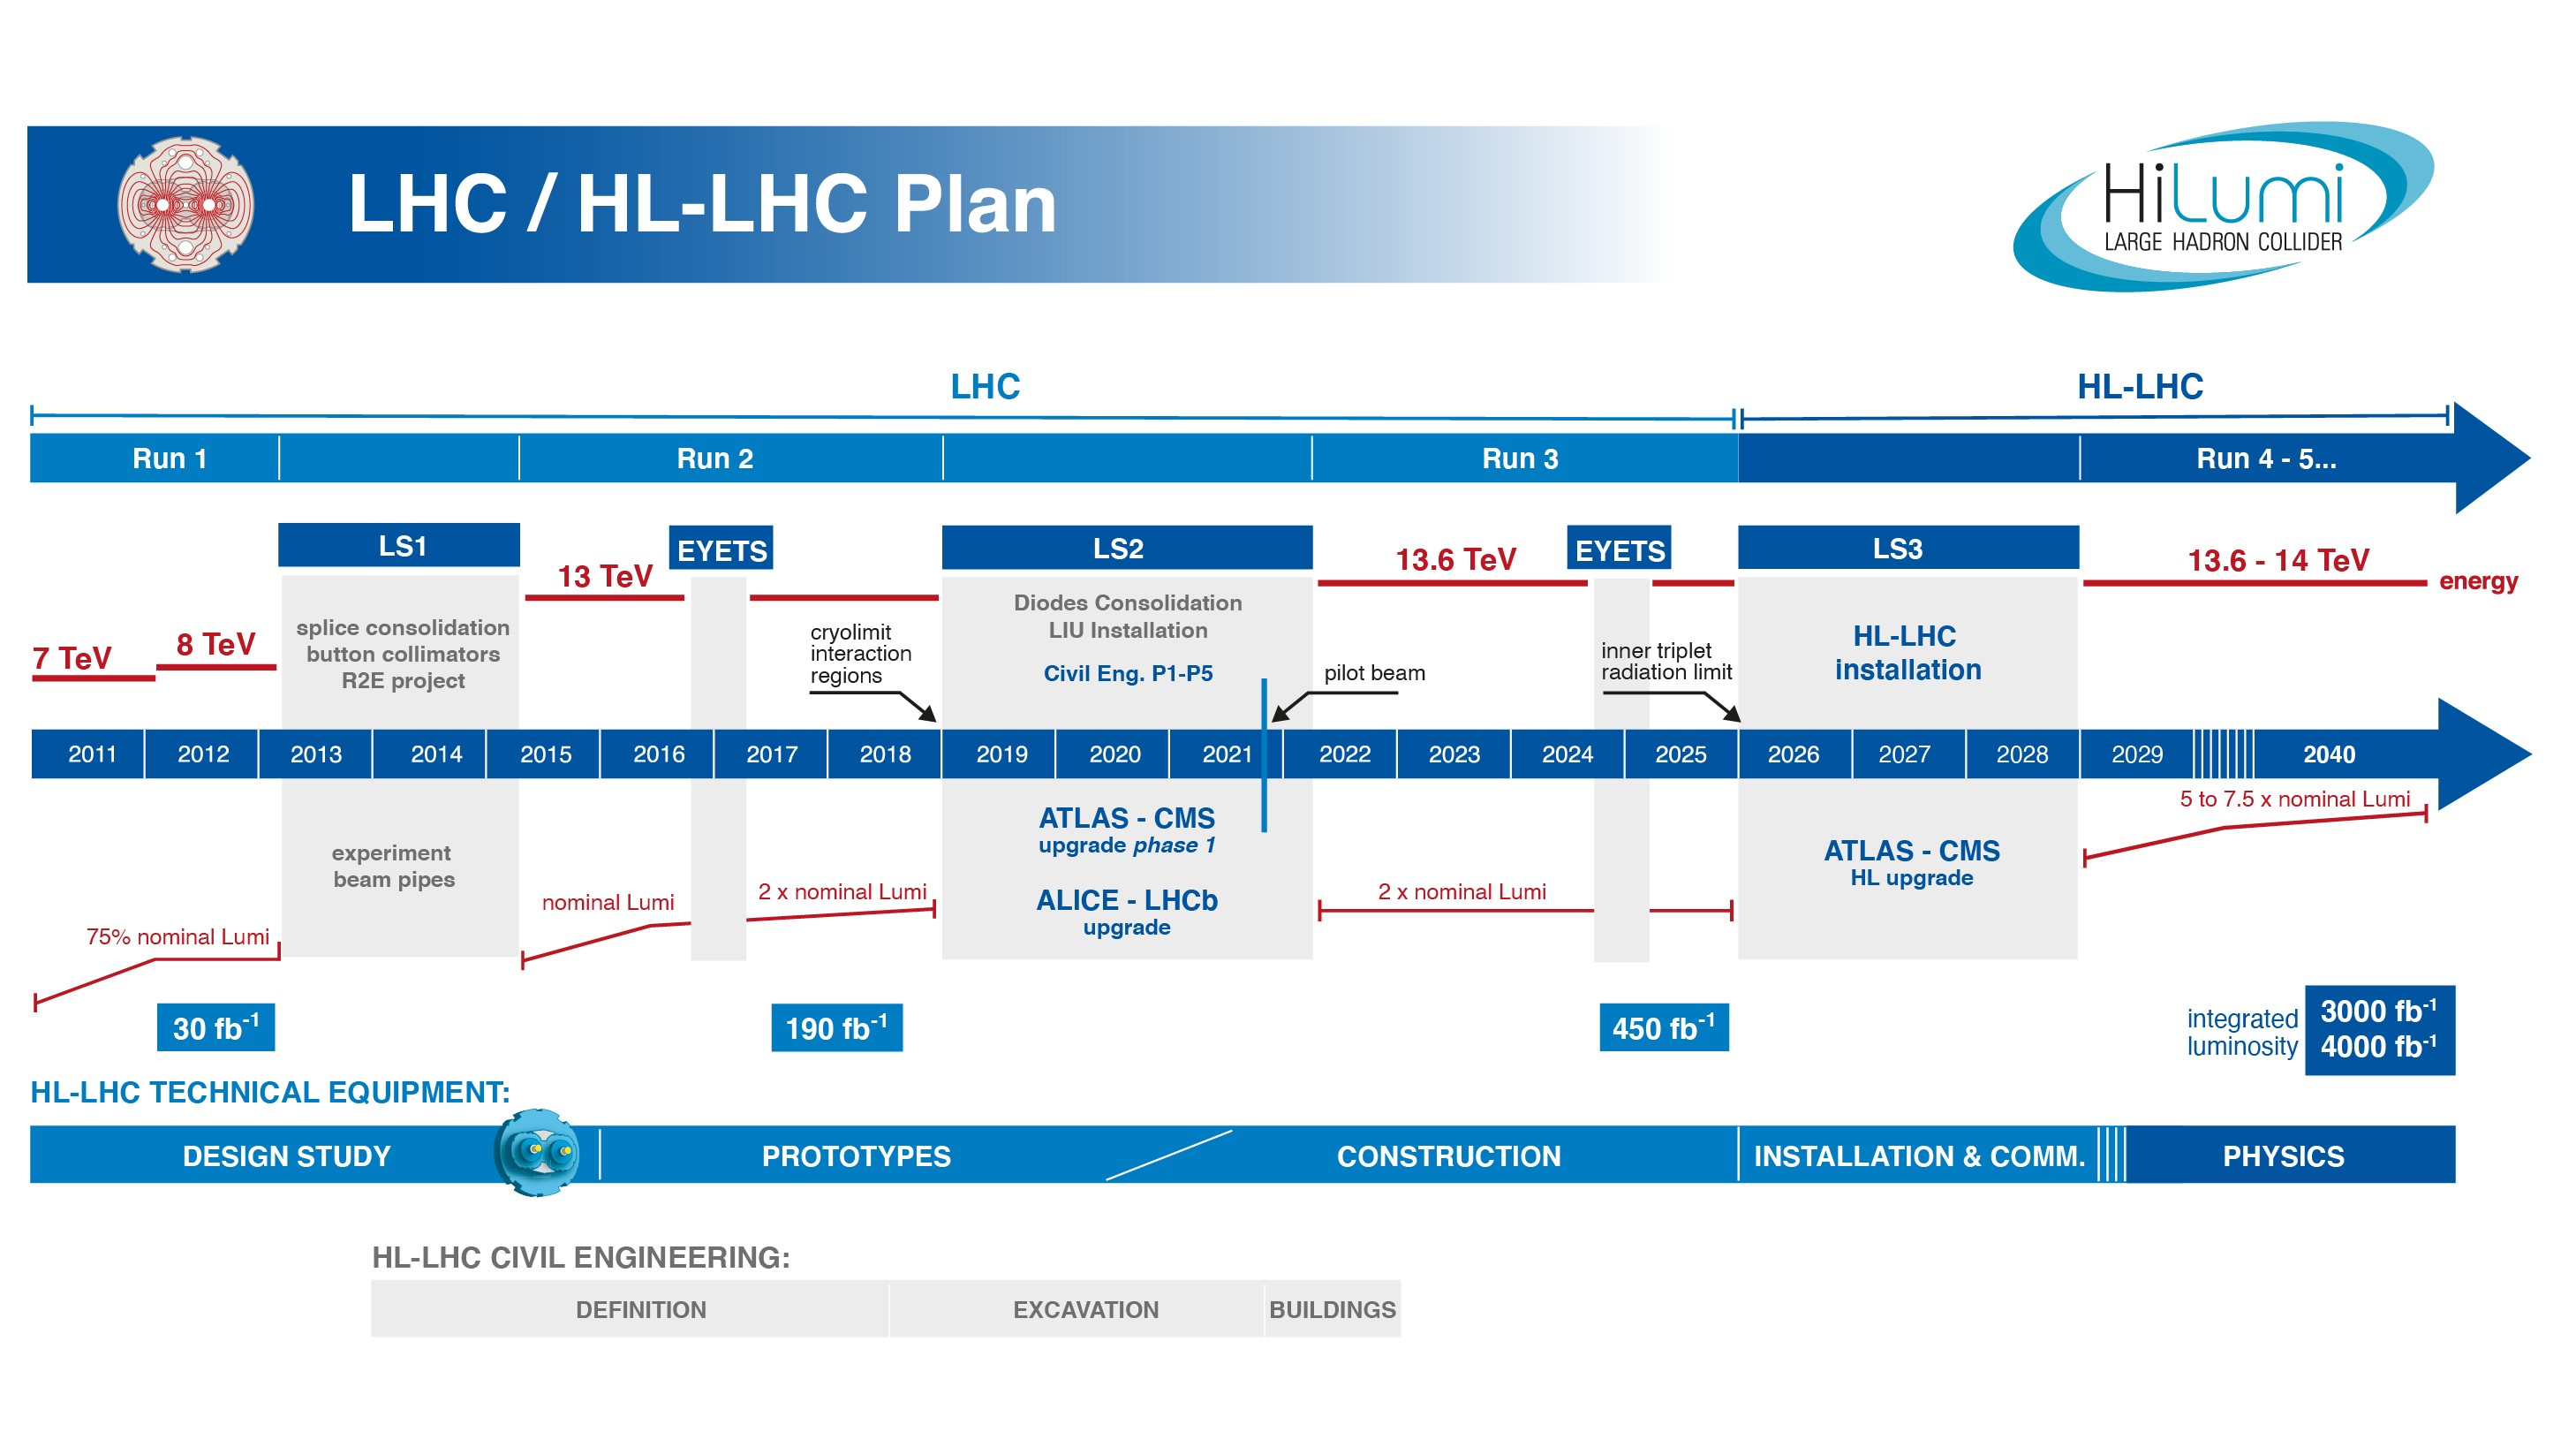
\includegraphics[width=.95\linewidth]{figures/LHC/HLLHCPlan.jpeg}
    \caption{ Timeline of LHC operation starting from 2011 to planned HL-LHC upgrade. Taken from \small{https://hilumilhc.web.cern.ch/content/hl-lhc-project}.\label{fig:HLLHC}}
\end{figure}
\normalsize

\subsection{ATLAS Upgrades}
\label{subsec:ATLASUpgrade}
At HL-LHC, about $200$ interactions per bunch crossing are expected, giving rise to several detector challenges, such as higher detector occupancy, harsher radiation conditions, and higher particle fluxes \cite{HLLHC}. The atlas detector will undergo a Phase-II upgrade to upgrade several sub-systems of ATLAS to meet the challenges of HL-LHC. The main upgrades include upgrading the muon system by adding new chambers in the inner barrel region, upgrading the trigger $\&$ data acquisition system to meet challenges from higher detector occupancy, and upgrading the electronics of several sub-systems. Additionally, a new High Granularity Timing Detector (HGTD) will also be inserted in the end-caps to supplement the tracking system and, most importantly replacement of the current ID with all Silicon Inner Tracking Detector (ITk) \cite{HLLHC}.

The ITk consists of Silicon pixel and strip detectors to increase granularity and radiation hardness with less material in the detector. Figure \ref{fig:ITKLayout} schematically shows the ITk layout with $5$ inner layers of pixel detector and four outer layers of strips detector. The tracking for ITk is extended in the forward region up to $|\eta| < 4.0$ region \cite{ITkStripsTDR}. 

\begin{figure}
    \centering
    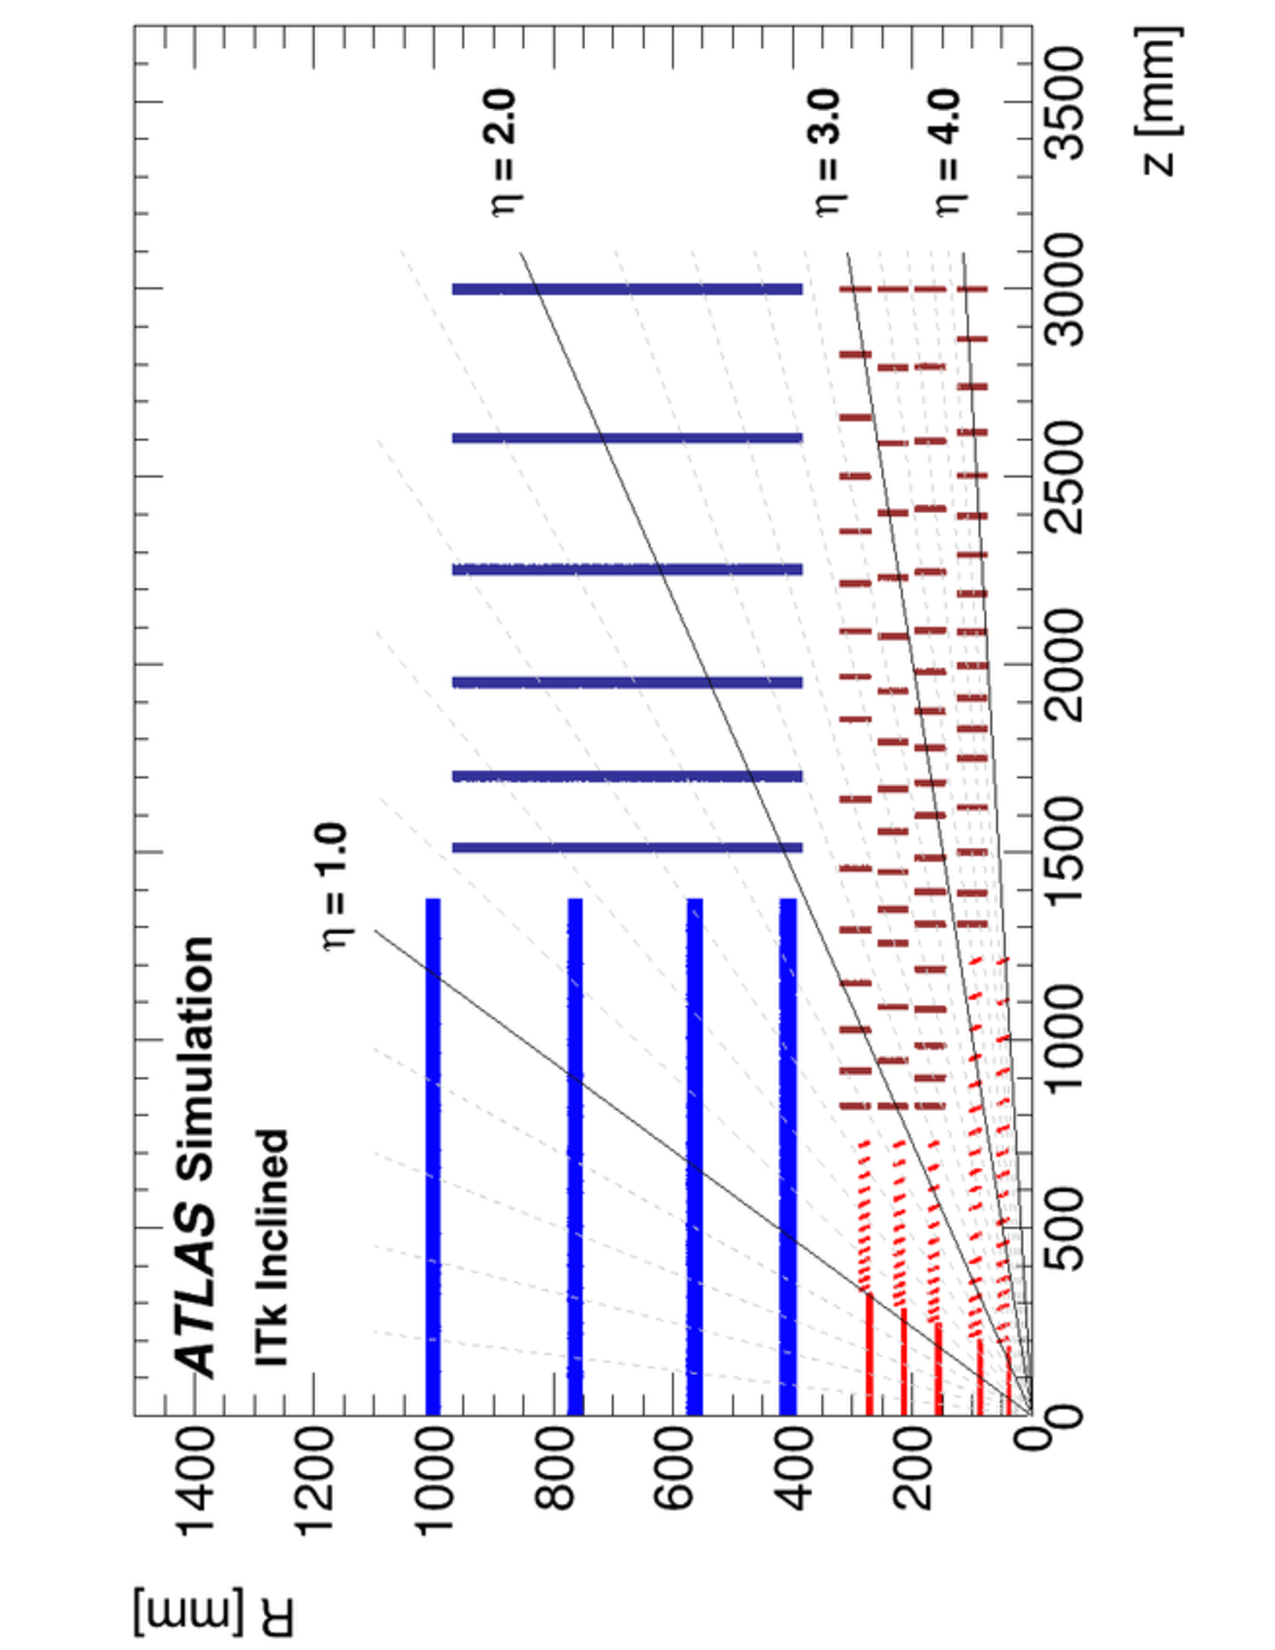
\includegraphics[angle=270,width=.95\linewidth]{figures/LHC/ITKLayout.pdf}
    \caption{ Schematic layout of ITK \cite{ITkPixelTDR}.\label{fig:ITKLayout}}
\end{figure}

More extensive statistics, extended tracking in the forward region, and the timing information from the HGTD HL-LHC program are highly beneficial to VBS $ZZjj$ measurements with extremely small cross-sections and two jets in the forward regions. 

	\section{ATLAS Detector}
\label{sec:ATLAS}

A Toroidal LHC ApparatuS (ATLAS) is a general-purpose detector of LHC that detects events from proton-proton and heavy ion collisions \cite{ATLAS}. It is a $44$ meters long, and $25$ meters wide cylindrical-shaped detector built around LHC Interaction Point 1 \cite{ATLAS}. ATLAS has multiple concentric sub-detectors layered around the beamline, providing forward-backward symmetric coverage. The two proton beams collide at the center of the detector producing outgoing particles from hard scattering, underlying events, and pile-up. The outgoing particles interact with the detector material leaving tracks and energy deposits in several layers of the sub-detectors. The sub-detector closest to the beamline is called \textit{Inner Detector (ID)}, which measures the trajectories of the charged particle and plays a crucial role in identifying the physical position of hard-scattering, also known as the \textit{interaction point (IP)}. ID is surrounded by a solenoid magnet that provides a $2$ T magnetic field to bend the particle trajectories for momentum measurements \cite{ATLAS}. After the solenoid magnet lies the \textit{electromagnetic calorimeter (ECAL)} and then the \textit{hadronic calorimeter (HCAL)}, which measure the energy of electromagnetic and hadronic physic objects, respectively. The outermost layer of the ATLAS detector is the \textit{Muon Spectrometer(MS)} that provides a secondary measure of muon trajectories for momentum measurement. MS is embedded inside a toroidal magnetic field that provides a magnetic field up to 3.5 T \cite{ATLAS}. Figure \ref{fig:ATLAS} shows a schematic of the ATLAS detector with all its sub-detectors.

\begin{figure}
    \centering
    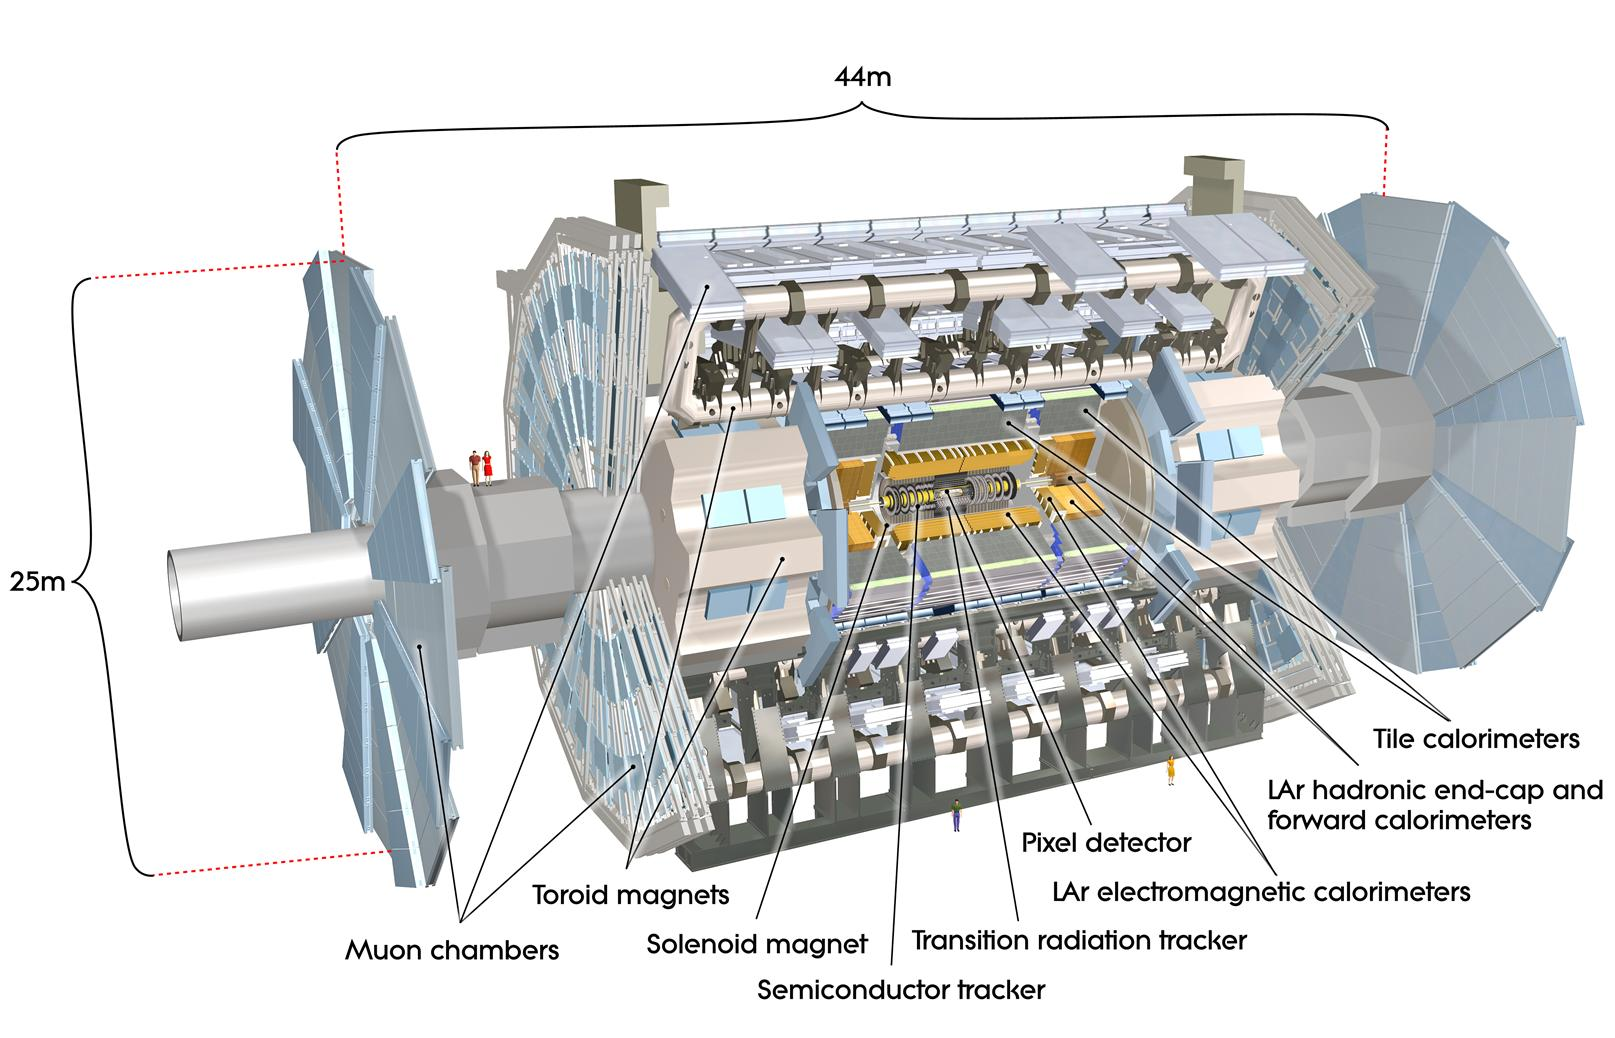
\includegraphics[width=.98\linewidth]{figures/LHC/AtlasDetector.png}
    \caption{ A detailed schematic of the ATLAS detector with all its sub-detectors \cite{ATLAS}.\label{fig:ATLAS}}
\end{figure}

\subsection{ATLAS Coordinate System}
\label{subsec:ATLASCS}

ATLAS measurements use a right-handed coordinate system with the nominal interaction point as the origin. The beamline is along the cylindrical symmetry axis of the detector, which defines the longitudinal \textit{z}-axis. The transverse \textit{xy}-plane is perpendicular to the beam direction, where \textit{x}-axis points to the center of the LHC ring and \textit{y}-axis points upwards towards the surface. Figure \ref{fig:ATLAS_CS} shows a schematic of the ATLAS coordinate system. The angle measured around the beamline in \textit{xy}-plane gives the azimuthal angle $\phi$, whereas the angle measured with respect to the \textit{z}-axis gives the polar angle $\theta$. Transverse momentum ($p_{T}$) is particle's momentum in the \textit{xy}-plane, defined as, 

\begin{equation}
p_{T} = \sqrt{p_{x}^2+p_{y}^2}=p\sin\theta
\label{eqn:pT}
\end{equation}
\textit{Rapidity (y)} defined in terms of a particle's energy ($E$) and momentum ($p$) is a commonly used collider physics quantity that measures whether an outgoing particle is produced perpendicular or parallel to the \textit{z}-axis. Rapidity is defined as, 

\begin{equation}
    y = \frac{1}{2}\ln{ \left( \frac{E+p_{z}}{E-p_{z}} \right) }
    \label{eqn:Rapidity}
\end{equation}
Particles with larger momentum along the \textit{z}-axis have larger values of rapidity, whereas particles with larger momentum values in the transverse plane have smaller values of rapidity. For particles with negligible mass, the rapidity approaches a purely angular variable called \textit{pseudorapidity ($\eta$)} defined as, 

\begin{equation}
    \eta = \frac{1}{2}\ln{ \left( \frac{ |\vec{p}|+p_{z}}{ |\vec{p}| -p_{z}} \right) } = -ln { \left[ \tan \left( \frac{\theta}{2}\right) \right] } 
    \label{eqn:PseudoRapidity}
\end{equation}
Higher values of rapidity and pseudorapidity refer to the forward region of the detector. ATLAS detector has full $2\pi$ coverage in $\phi$ and maximum coverage up to $|\eta| < 4.5$ corresponding to $1.3^{\circ} < \theta < 178.7^{\circ} $ \cite{ATLAS}. 

\begin{figure}
    \centering
    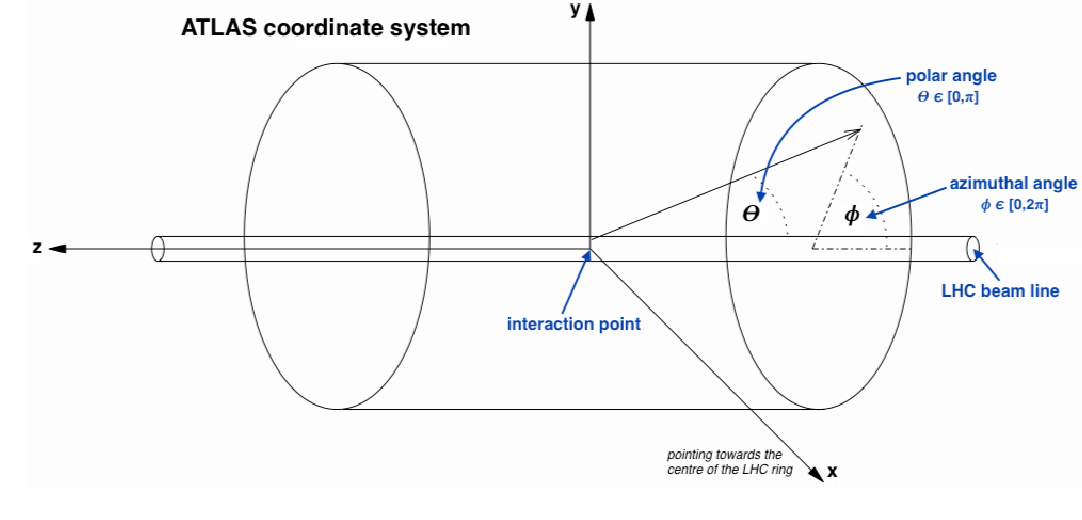
\includegraphics[width=.98\linewidth]{figures/LHC/ATLAS_CoordinateSys.png}
    \caption{ A schematic of the right-handed ATLAS coordinate system \cite{ATLAS_CoordSys}.\label{fig:ATLAS_CS}}
\end{figure}

\subsection{Inner Detector}
\label{subsec:ID}
The inner detector is the innermost sub-detector of ATLAS and is responsible for tracking charged particles' trajectories and identifying the interaction point of the hard scatter. Closest to the interaction point is the Insertable B-Layer (IBL) \cite{ATLAS_IBL}, which was installed during the long-upgrade shutdown between Run-1 and Run-2 to meet the requirements for competent tracking at higher pile-up. The IBL is highly granular, consisting of roughly 12 million silicon pixel sensors with a size of $50\times 250 ~\mu m^2$ \cite{ATLAS_IBL}. IBL is located $3.3$ cm from the beamline and can reconstruct tracks within the pseudorapidity range of $|\eta|<2.5$ \cite{ATLAS_IBL}. 

Three layers of silicon-pixel detectors with $1,744$ pixel sensors, each comprising $47,232$ pixels of size $50\times 400 ~\mu m^2$ surround the IBL \cite{ID_Pixel}. The slightly larger pixel size is adequate for the pile-up at a distance larger than $5$ cm from the interaction point. These pixel layers were also present during the Run-1 data-taking period and provided coverage up to $|\eta|<2.5$ with a spatial resolution of tracks between $5$ and 12 $\mu$m \cite{ID_Pixel}. Surrounding the pixel layers is the Semiconductor Tracker (SCT) consisting of five layers of silicon microstrip detectors with a mean strip pitch of $80 ~\mu m$ in the barrel region and varying pitch of  $57-94 ~\mu m$ in the end-cap regions \cite{ID_Strips}. 

At a distance about $50$ cm from the beamline lies the outermost layer of the ATLAS inner detector, the Transition Radiation Tracker (TRT), with $370,000$ straw tubes with a diameter of $4$ mm \cite{ID_TRT}. Each TRT straw tube is filled with a Xenon-based gas mixture and consists of $31~\mu m$ diameter tungsten wires \cite{ID_TRT}. A charged particle passing through different layers of ID leaves a track via ionization. 

Figure \ref{fig:ATLAS_ID} schematically shows different parts of the inner detector and their distances from the interaction point.

\begin{figure}
    \centering
    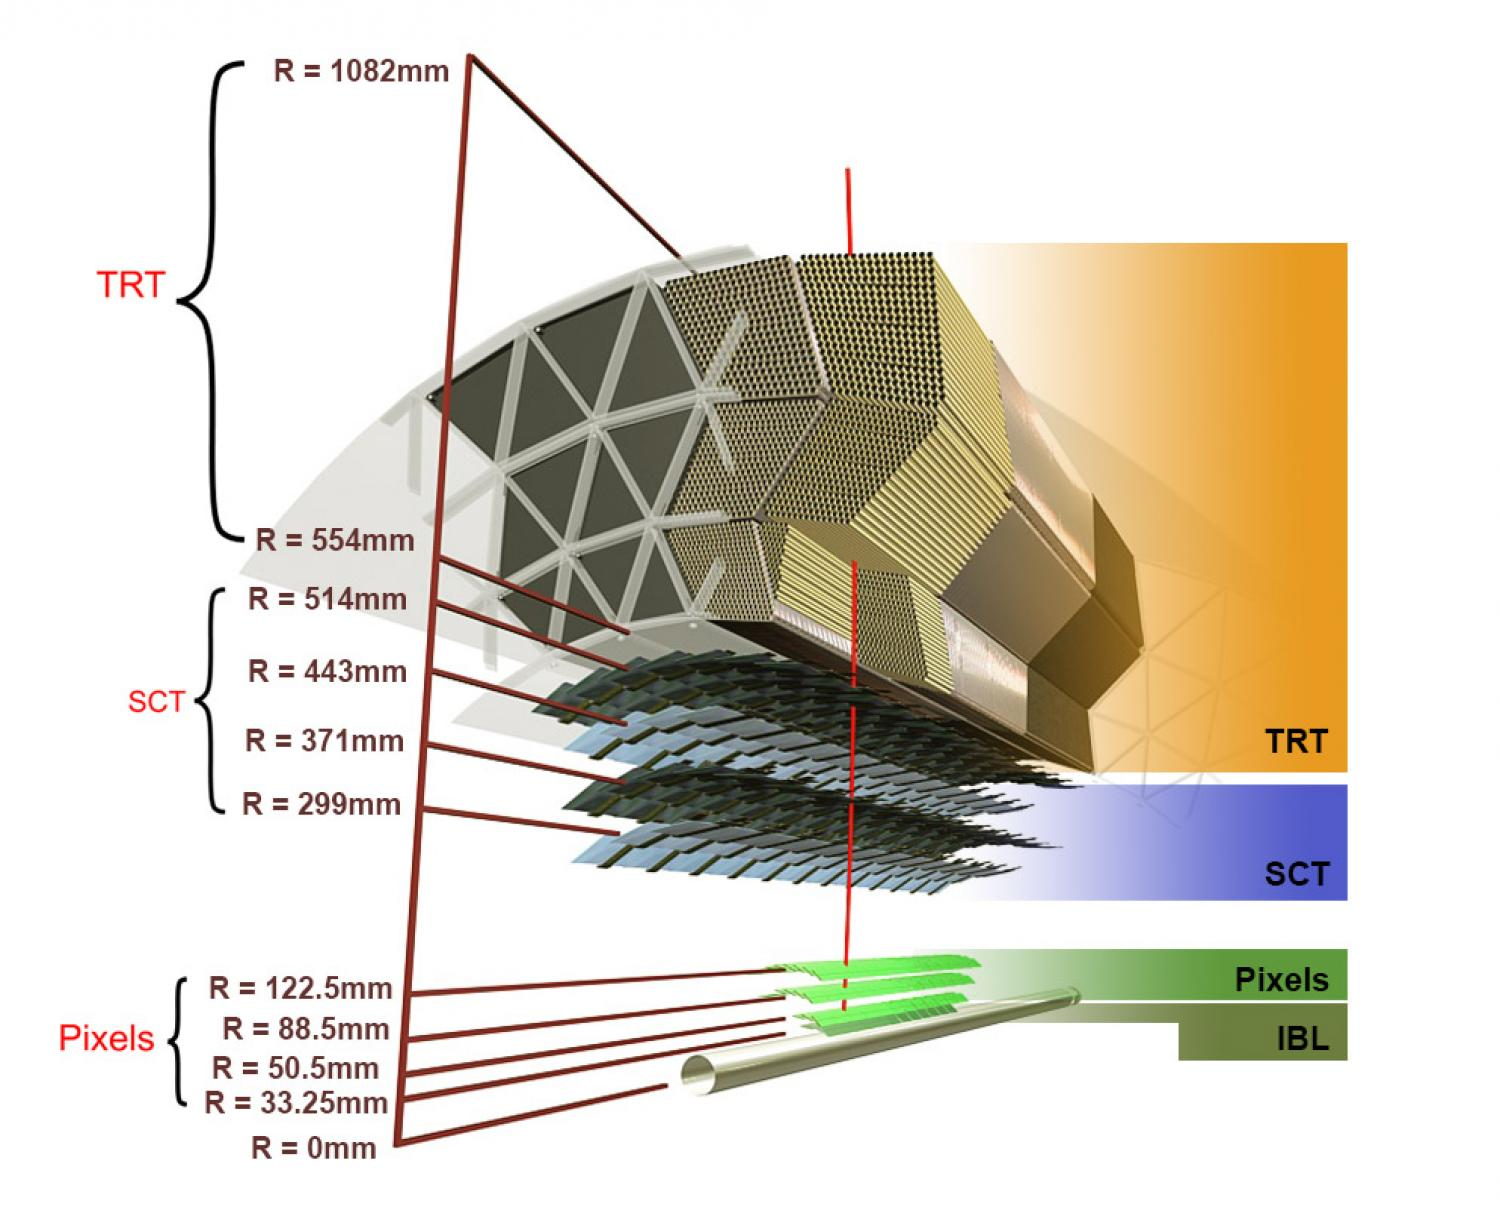
\includegraphics[width=.98\linewidth]{figures/LHC/ATLAS_InnerDetector.jpg}
    \caption{ A schematic of the inner detector of ATLAS showing the IBL, pixel detectors, SCT, and TRT \cite{ID_Align_Run2}.\label{fig:ATLAS_ID}}
\end{figure}

\subsection{Calorimeters}
\label{subsec:Cal}

ATLAS has two calorimeters, electromagnetic and hadronic, designed to measure the energy of charged and neutral particles up to the range of $|\eta|\leq4.9$ \cite{ATLAS}. When interacting with a material, an electron loses its energy by photon emission, which could produce a pair of $e^{+}e^{-}$ and vice versa, creating an electromagnetic shower in the detector. Similarly, the hadronic particles also result in a shower of particles through multiple scattering. The calorimeters measure the energy of the particles by reconstructing the electromagnetic and hadronic showers. The calorimeters are designed to capture all particles except muons and neutrinos. Therefore, motivated by the need to prevent \textit{punch-through}\footnote{particles' probabilities of passing through the calorimeters} effect, materials with high radiation length ($X_{0}$) and high interaction length ($\lambda$) are chosen to construct the calorimeters.

Outside the solenoid magnet surrounding the ID is the accordion-shaped electromagnetic calorimeter consisting of an alternate layer of lead absorber plates and highly granular liquid-argon (LAr) cells to precisely measure the energies of electrons and photons. It comprise of barrel section in $|\eta| < 1.475$ range and two end-caps in $1.375 < |\eta| < 3.2$ range \cite{ATLAS_ECAL}. The calorimeter's central region ($|\eta| < 2.5$) is designed to identify electrons and photons with high precision.

The hadronic calorimeter surrounds the ECAL and consists of a steel absorber and active scintillator tiles in the $|\eta| < 1.7$ range. In the end-caps range of $1.5 < |\eta| < 3.2$, it consists of a copper absorber and active LAr detectors. The forward region ranging from $3.2 < |\eta| < 4$ comprises the tungsten absorber followed by active LAr detectors \cite{ATLAS_HCAL}. 

Figure \ref{fig:ATLAS_Cals} schematically shows the layout of ATLAS calorimeters. 

\begin{figure}
    \centering
    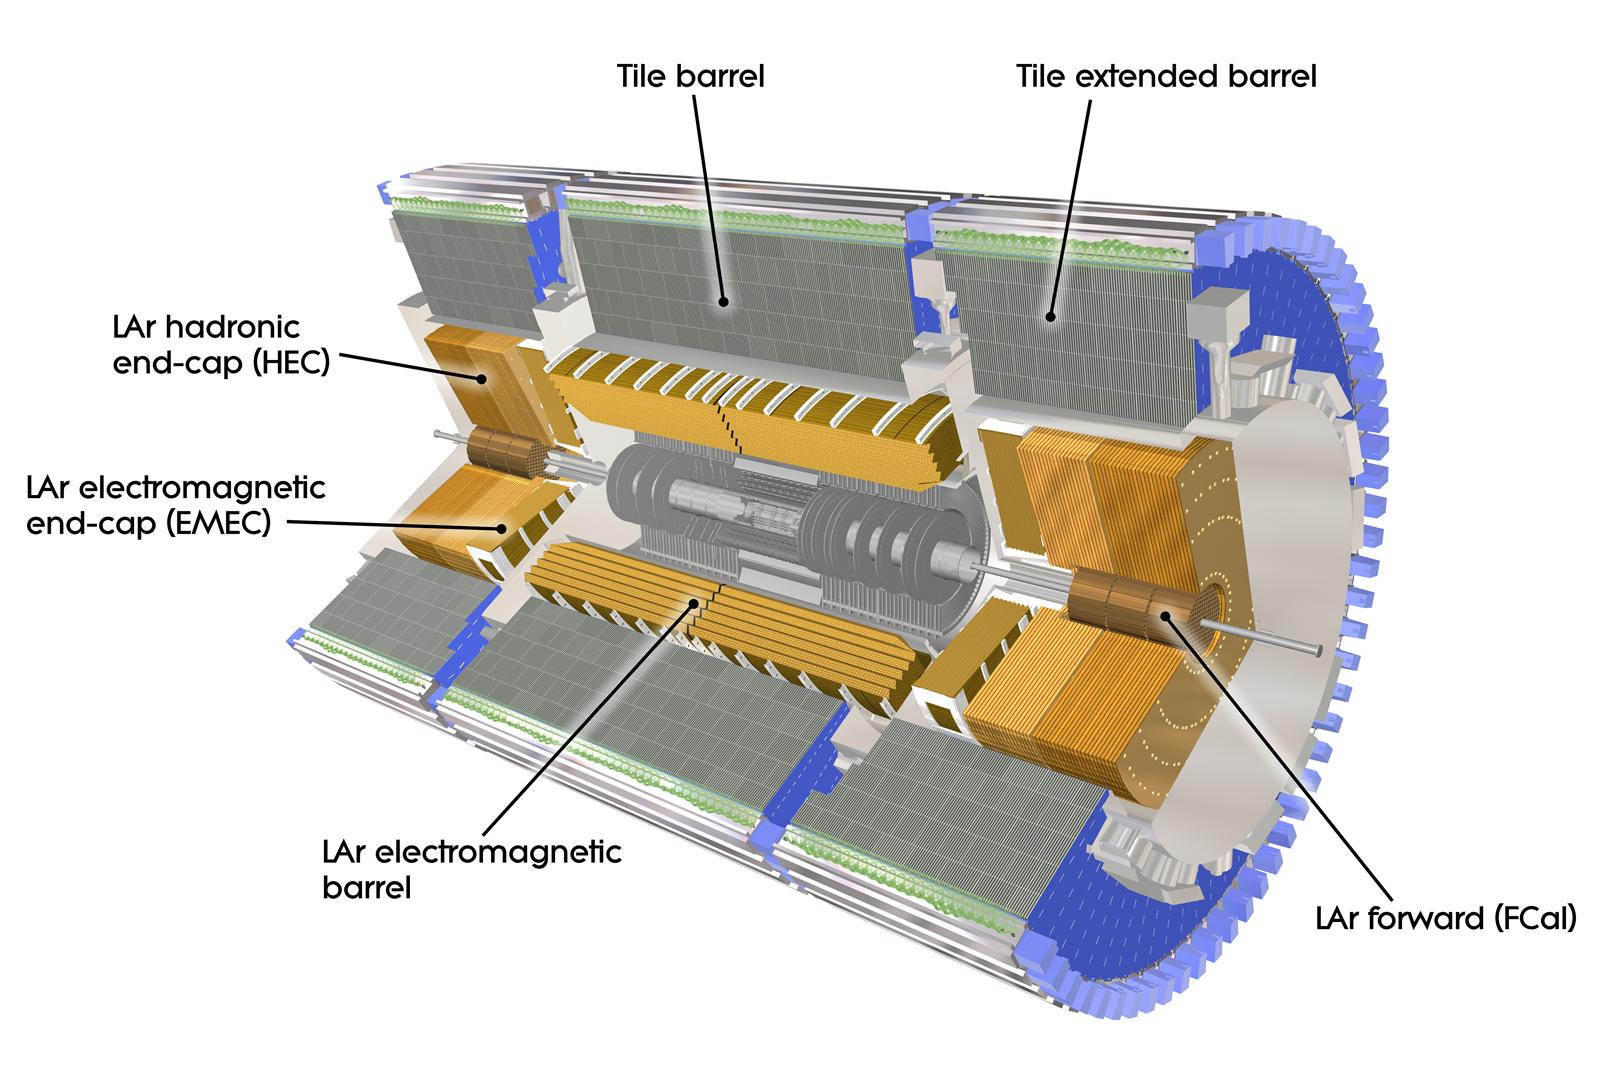
\includegraphics[width=.98\linewidth]{figures/LHC/ATLAS_CALO.jpeg}
    \caption{ A schematic of electromagnetic and hadronic calorimeters In ATLAS \cite{ATLAS}.\label{fig:ATLAS_Cals}}
\end{figure}

\subsection{Muon Spectrometer}
\label{subsec:MS}
In ATLAS, muons are deeply-penetrating charged particles that leave minimum ionizing deposits in the calorimeter. The muon spectrometer, the outermost part of the ATLAS detector, tracks trajectories of muons deflected in $0.5$ magnetic field provided by the superconducting toroidal magnets, giving an additional measure of muon's momentum \cite{ATLAS}. The MS tracks muon with $p_{T} > 3$ GeV in $|\eta| < 2.7$ range \cite{ATLAS}. As shown in figure \ref{fig:ATLAS_MS}, the muon spectrometer comprises four types of detectors; first, the three stations of Monitored Drift Tubes (MDT) in $|\eta| < 2.0$ region followed by the Cathode Strip Chambers (CSC) in  $2.0 < |\eta| < 2.7$ region \cite{ATLAS}. The other two detectors are the Resistive Plate Chambers (RPC) in $|\eta| < 1.05$ and the Thin-gap Chambers (TGC) beyond $|\eta| = 1.05$ comprising the trigger system in MS \cite{ATLAS}. 

\begin{figure}
    \centering
    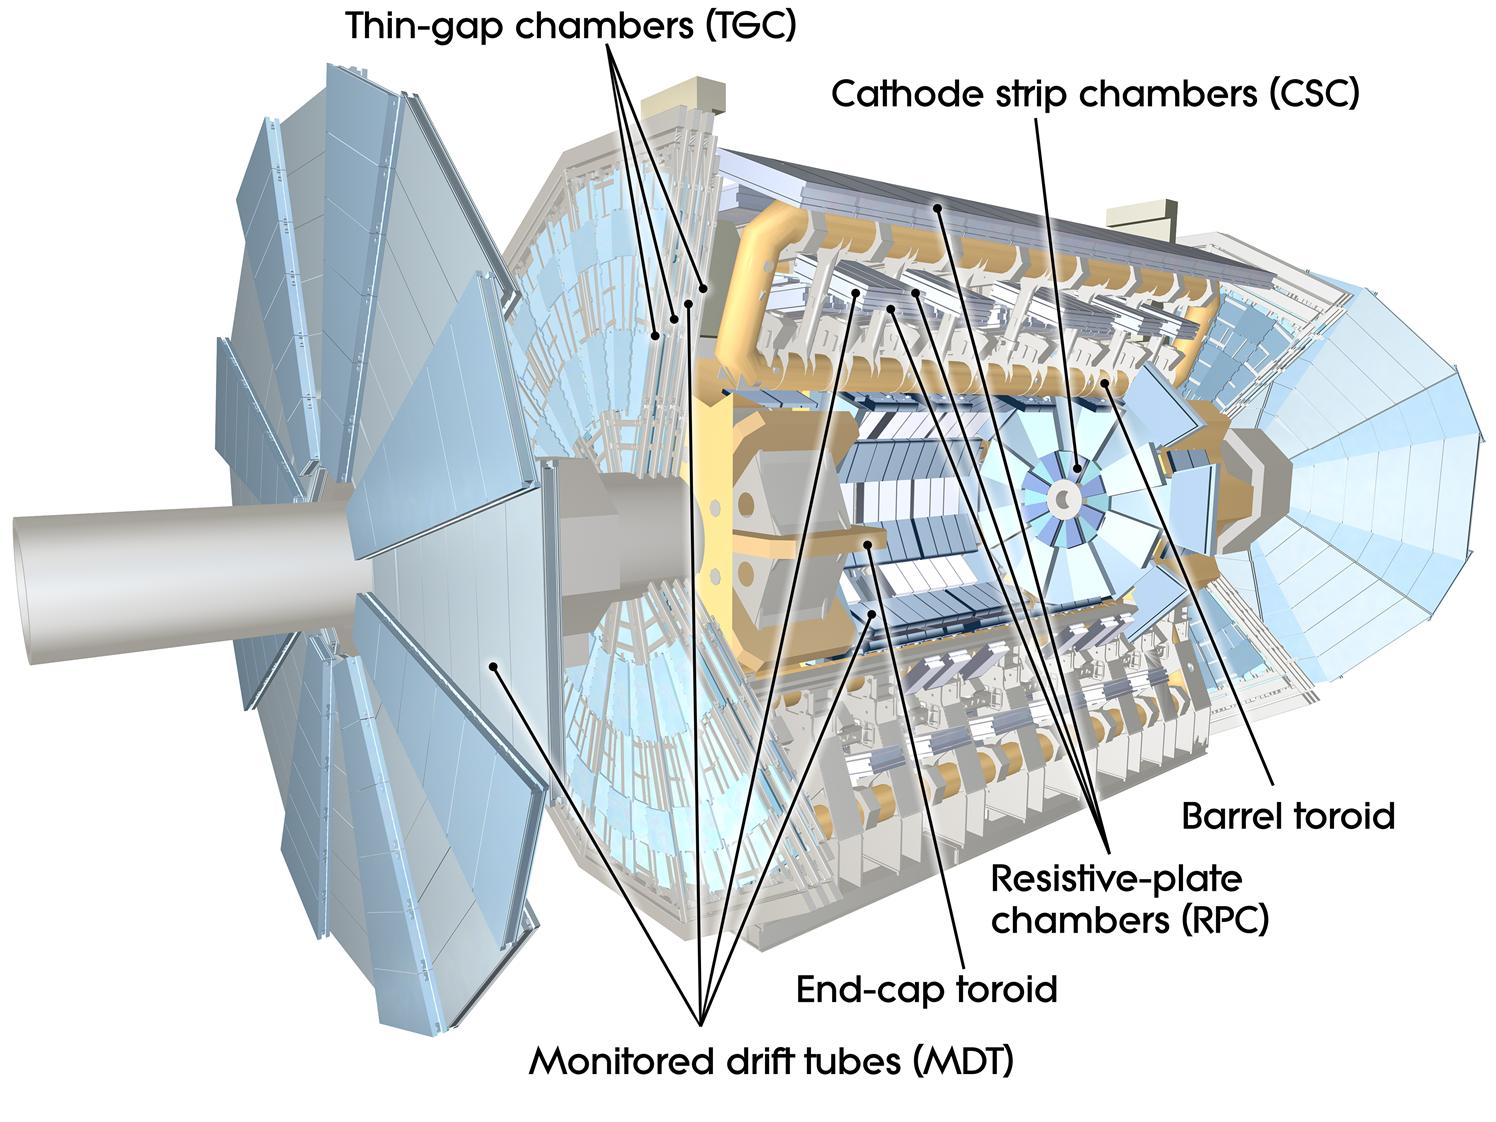
\includegraphics[width=.98\linewidth]{figures/LHC/ATLAS_MS.jpeg}
    \caption{ A schematic of different components of the muon spectrometer in ATLAS \cite{ATLAS}.\label{fig:ATLAS_MS}}
\end{figure}
	\section{ Physics Object Reconstruction} 
\label{sec:ParticleReconstruction}
Different particles leave unique signatures in different sub-detectors of ATLAS. Figure \ref{fig:ATLASTransverse} shows a schematic of simplified representation of various particles passing through different sub-detectors and leaving various signature. Physics object reconstruction is the process of interpreting these signals to meaningful information about the outgoing particles. This section discusses the detail of reconstruction relevant to the thesis. 

\begin{figure}
    \centering
    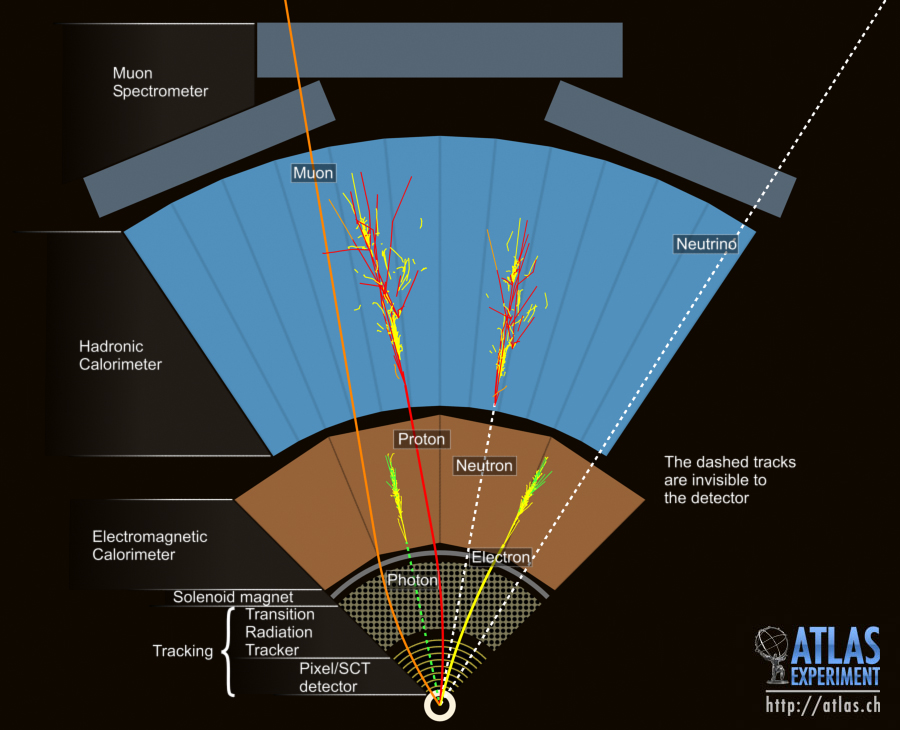
\includegraphics[width=.98\linewidth]{figures/LHC/ATLAS_Transverse.jpg}
    \caption{ Simplified representation of various particles traversing through different layers of ATLAS sub-detectors and leaving unique signatures \cite{ATLASTransverse}.\label{fig:ATLASTransverse}}
\end{figure}

\subsection{Trigger}
\label{subsec:TriggerATLAS}
The first step of particle and event reconstruction is selecting interesting high-energy events from a pool of lower-energy multiple-scattering signals. The high bunch crossing frequency of every $25$ ns results from a large amount of data making it physically impossible to store all events. ATLAS trigger system selects the events interesting for physics objects. 

ATLAS trigger consists of two levels, Level 1 (L1) trigger integrated into the hardware and high-level software trigger (HLT) \cite{TriggerSystemATLAS}. The L1 trigger is based on custom-built electronics, which uses signals from the calorimeters and muon trigger system (TGC and RPC) to identify event features such as electrons, photons, jets, taus, and missing energy. The L1 trigger reduces the $40$ MHz incoming collision data-rate corresponding to $25$ ns bunch crossing by a factor of $400$ to $100$ kHz output \cite{TriggerSystemATLAS}. The events accepted by the L1 trigger defines regions of interest (ROI), and HLT algorithms are run on these events to select ones with candidate physics objects and kinematic requirement. The software-based HLT trigger further reduces the data rate by almost a factor of 100 to $1.5$ kHz \cite{ATLAS}. With the combination of L1 and HLT trigger system, the data rate is reduced by $400,000$, and the selected events corresponding to data readout of $1.5$ GB are stored in the permanent storage. Figure \ref{fig:DAQ} shows the schematic of ATLAS's trigger and data acquisition system. 

\begin{figure}
    \centering
    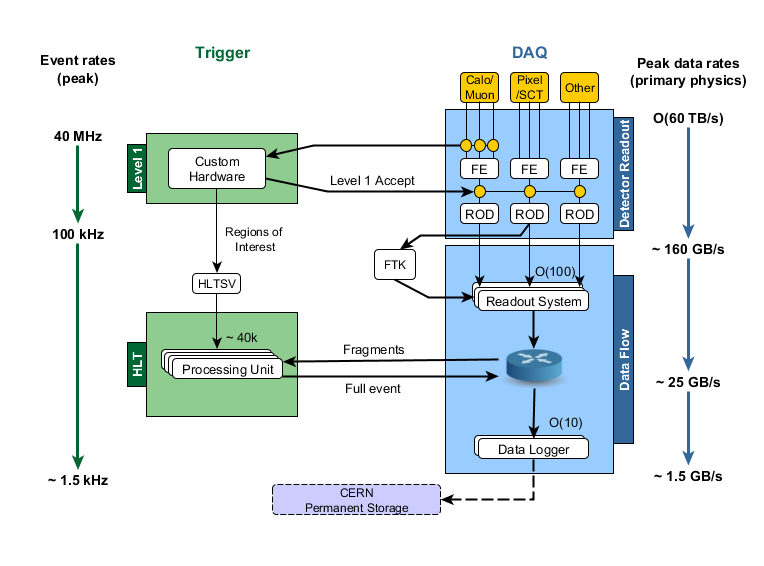
\includegraphics[width=.98\linewidth]{figures/LHC/DAQ_ATLAS.png}
    \caption{ Trigger and data acquisition system in ATLAS \cite{ATLAS_DAQ}.\label{fig:DAQ}}
\end{figure}

Physics object reconstruction discussed below converts the raw data output stored in permanent storage to physics objects used in physics analyses. 

\subsection{Tracks and Vertices Reconstruction}
\label{subsec:Tracking}
Tracking a charged particle is a critical step in reconstruction. The tracks of the charged particles play an essential role in momentum measurement, particle identification, and primary vertex reconstruction through the extrapolation of tracks to the interaction point. As the inner detector is closest to the beamline and comprises minimally ionizing detector material with high granularity, it plays a crucial role in track reconstruction. The ID magnetic field is homogenous, resulting in circular tracks of the charged particles. Five parameters define charged particle tracks; the ratio of charge and transverse momentum ($q/p_{T}$) defining the curvature; the distance of the closest approach to the primary vertex in $xy$-plane defining the transverse impact parameter ($d_{0}$), the longitudinal impact parameter ($z_{0}$) along the $z$-axis; the azimuthal angle ($\phi_{0}$) and the polar angle ($\theta_{0}$) of the particle direction at the closest approach point \cite{TrackingRun2_ATLAS}. Figure \ref{fig:TrackParameter} schematically shows the five-track parameters. 

\begin{figure}
    \centering
    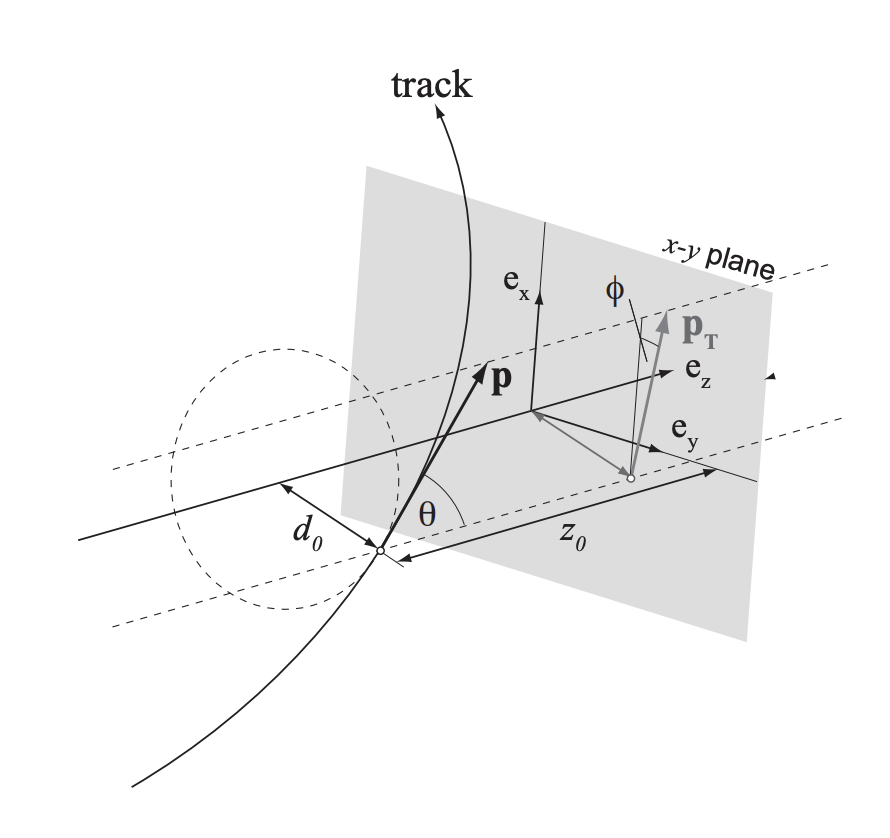
\includegraphics[width=.98\linewidth]{figures/LHC/TrackParameters.png}
    \caption{ Schematic showing the five-track parameters \cite{TrackParameterFig}.\label{fig:TrackParameter}}
\end{figure}

As shown by figure \ref{fig:TrackingOutline}, track reconstruction follows two different approaches used in Run-2; the primary \textit{inside-out} approach and the secondary \textit{outside-in} approach \cite{TrackingRun2_ATLAS}. The first step in the inside-out track reconstruction is the space point and drift circle formation, formed respectively by the clusters of signals from the silicon detectors and drift-circles hits in the TRT. Second, track seeds are formed from a collection of three silicon-detector space points and extrapolated to the outer layers by including the compatible clusters in the track trajectory. Once the track is formed, an ambiguity resolution algorithm is applied to reassign shared clusters to the track with a better match, and the final track candidate is fitted using a global $\chi^{2}$ method. The last step of inside-out track reconstruction is adding compatible TRT drift holes and refitting the tracks. 

\begin{figure}
    \centering
    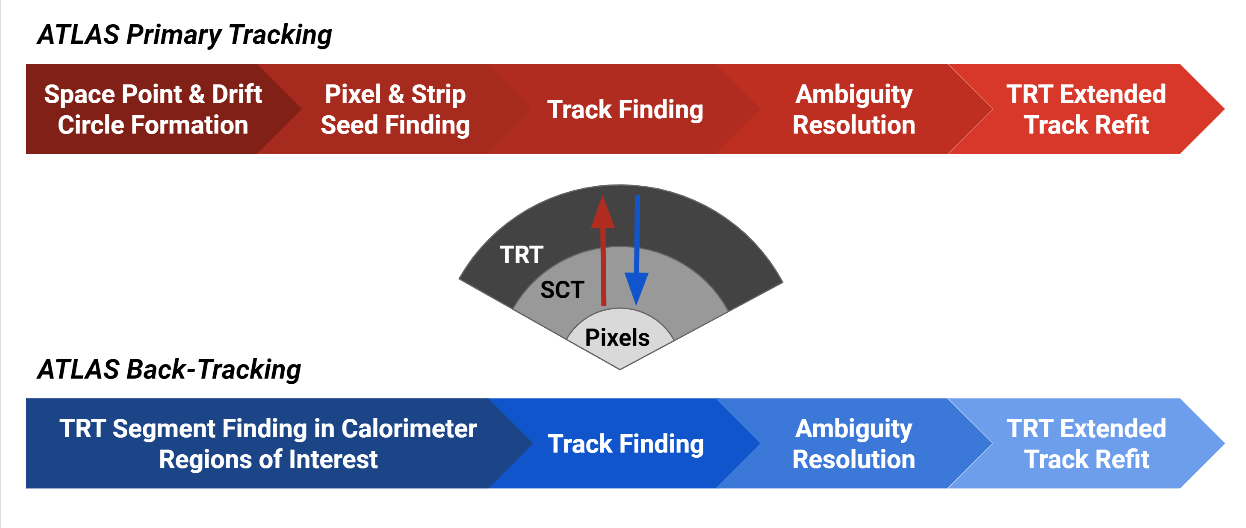
\includegraphics[width=.98\linewidth]{figures/LHC/trackingflowchart.png}
    \caption{schematic showing the two types of track reconstruction, primary inside-out and secondary outside-in. Taken from ATLAS Tracking CP group public tutorial \url{https://atlassoftwaredocs.web.cern.ch/trackingTutorial/idoverview/}. \label{fig:TrackingOutline}}
\end{figure}

The inside-out method is optimal for particles that minimally interact with the inner-detector material. However, secondary backtracking with an outside-in approach is needed for particles interacting with the inner detector, such as reconverted photons. In this approach, the track pattern recognition starts at the TRT in the regions of interest flagged by the electromagnetic calorimeter and backtracks to the silicon detectors. 

Tracks of the charged particle are extrapolated inward to the beamline and are assigned to vertices \cite{VertexReconstruction}. In most ATLAS analyses, including the one presented in this thesis, the space-point with the highest quadrature sum of track $p_T$ ($\sum_{track}{p_{T}^2}$) is identified as the primary vertex of an event.

\subsection{Electron Reconstruction}
\label{subsec:ParticleRecon_Elec}
Electrons, when interacting with a material, produce a photon by bremsstrahlung radiation, the process defining the interaction of a charged particle with the electric field of an atomic nucleus. Any energetic photon, either from a physics process or bremsstrahlung, can turn into a pair of $e^{+}e^{-}$, which can again radiate another set of photons, thus, giving rise to an electromagnetic shower. For given energy and material, electromagnetic showers have a characteristic penetration depth.

ATLAS electrons are reconstructed by combining the tracking information from the ID, and the energy deposits in nearby cells of the calorimeter,  energy clusters \cite{ElectronReco}. The clusters are formed only if the energy deposit exceeds four times the expected deposits from the pile-up. The reconstruction efficiency for high-energy electrons with transverse energy ($E_{T}>15$ GeV) is about $97-99\%$ \cite{ElectronReco}. \textit{Prompt electrons} originate from the hard scattering and are the primary interest of physics analysis. However, the detector has electrons from \textit{non-prompt sources} including the jets, misidentification, and pile-up. Therefore it is imperative to identify and isolate the prompt electrons in an event, and the efficiency for identification and isolation varies as a function of $E_{T}$. Limited by the coverage of the electromagnetic calorimeter, only electrons within the $|\eta| <2.47$ range can be reconstructed and identified as prompt in ATLAS.

The electron identification is based on a multivariate-likelihood (LH) technique which takes information from tracking detectors and calorimeters as input. The tool is trained to separate signal and background probability density functions using simulated $Z \rightarrow ee$ and $Z \rightarrow J / \psi$ events. The LH tool provides four \textit{working points}, VeryLoose, Loose, Medium, and Tight, at different values of the LH discriminant to cover various needs of several ATLAS analyses. The analysis presented in this thesis uses electrons satisfying the Loose identification working point with at least one hit in the IBL. 

Prompt electrons originating from W, Z, or H decay are characterized by low activity around them in the $\eta-\phi$ plane. An isolation requirement is applied to the electron candidates to select ones from the hard scattering. Calorimeter and track-based requirements on isolation variables are defined to quantify the isolation. The variables are based on the amount of activity around an isolation cone of the candidate electron. Calorimeter-based isolation relies on the variable $E_{T,cone}^{iso}$, the sum of transverse energies inside a $\deltaR=0.2$ cone of the electron candidate. Similarly, the track-based isolation variable is $p_{T,cone}^{iso}$, the sum of the transverse momentum of the electron candidate within a $p_{T}-$dependent $\Delta R$, which is defined as, 

\begin{equation}
\Delta R = min \left( \frac{10 GeV}{p_{T}},\Delta R_{max} \right)
\end{equation}

where the maximum cone size is $\Delta R_{max} = 0.2$. Similar to the identification, several working points are available for electron isolation. The measurement in this thesis uses the \textit{Loose$\_$VarRad} isolation working point which requires $E_{T,cone}^{iso} < 0.3$ and $p_{T,cone}^{iso} < 0.15$. Figure \ref{fig:ElecEff} shows the electron identification and isolation efficiencies as a function of their $E_{T}$. The Loose working point has the highest identification and isolation efficiencies and is the optimal working point for the measurement because of the fully reconstructable final state.

\begin{figure}
    \centering
    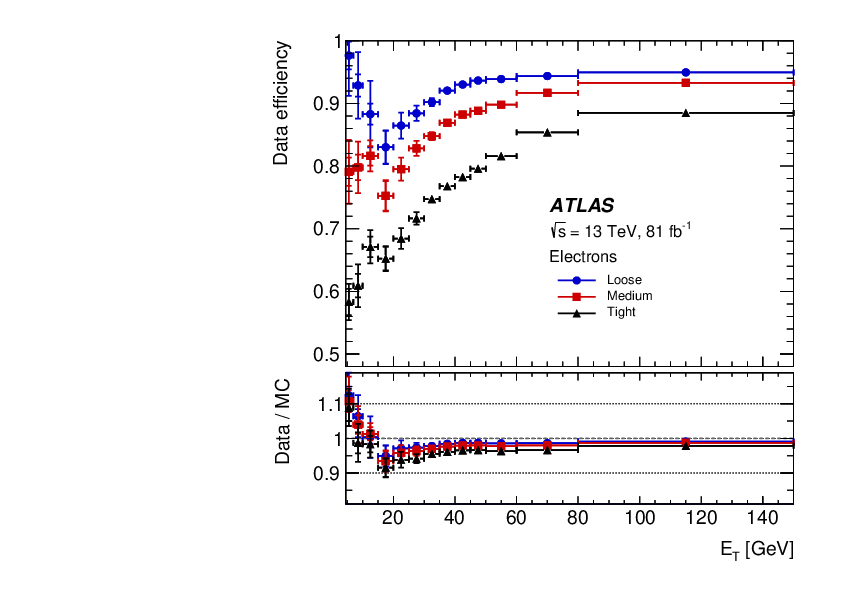
\includegraphics[width=.49\linewidth]{figures/LHC/ElecIdent_Eff.png}
    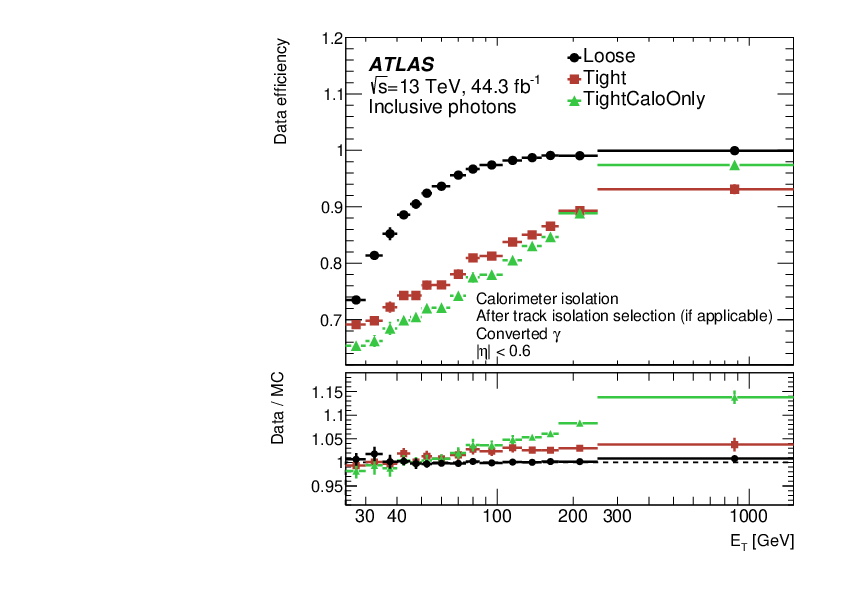
\includegraphics[width=.49\linewidth]{figures/LHC/Elec_IsoEff.png}
    \caption{ Distributions showing the identification (left) and isolation (right) efficiencies for electrons as a function of their $E_{T}$\cite{ElectronReco}.\label{fig:ElecEff}}
\end{figure}

The total electron efficiency is defined as the product of the electron reconstruction, identification, isolation, and trigger efficiencies as, 

\begin{equation}
    \epsilon_{total} = \epsilon_{reco} \times \epsilon_{id} \times \epsilon_{iso} \times \epsilon_{trigger}     
\end{equation}

Each of the efficiency terms is evaluated on data and MC. \textit{Scale Factors (SF)} defined as the ratio of the measured efficiency in data and the efficiency simulated in MC are derived and applied to the simulation to match the one observed in the data. Typically, SFs are close to one, and systematic uncertainties related to scale factors are considered in the measurement.

\subsection{Muon Reconstruction}
\label{subsec:ParticleRecon_Muon}
The rate of bremsstrahlung radiation is inversely proportional to the square of a particle's mass. Since muons are about $200$ times heavier than electrons, they primarily interact with the detector material through ionization. Therefore, muons are minimally ionizing particles that do not create electromagnetic shower in the calorimeters and pass through all layers of the ATLAS detector. Hence, muon detection relies on track measurements from the inner detector and muon spectrometer. As shown in figure \ref{fig:MuonFig}, four types of muons are defined based on the type of sub-detectors used during a muon reconstruction,

\begin{itemize}
    \item{\textbf{Combined muons:} muons reconstructed from a global refit of ID and MS tracks }
    \item{\textbf{Segment-tagged muons:} muons reconstructed from a fitted ID track and MS segment track } 
    \item{\textbf{Calo-tagged muons:}  muons reconstructed using ID track matched to the minimum ionizing energy deposits in the calorimeters}
    \item{\textbf{Standalone Muons:} muons reconstructed solely from the MS tracks }
\end{itemize}

\begin{figure}
    \centering
    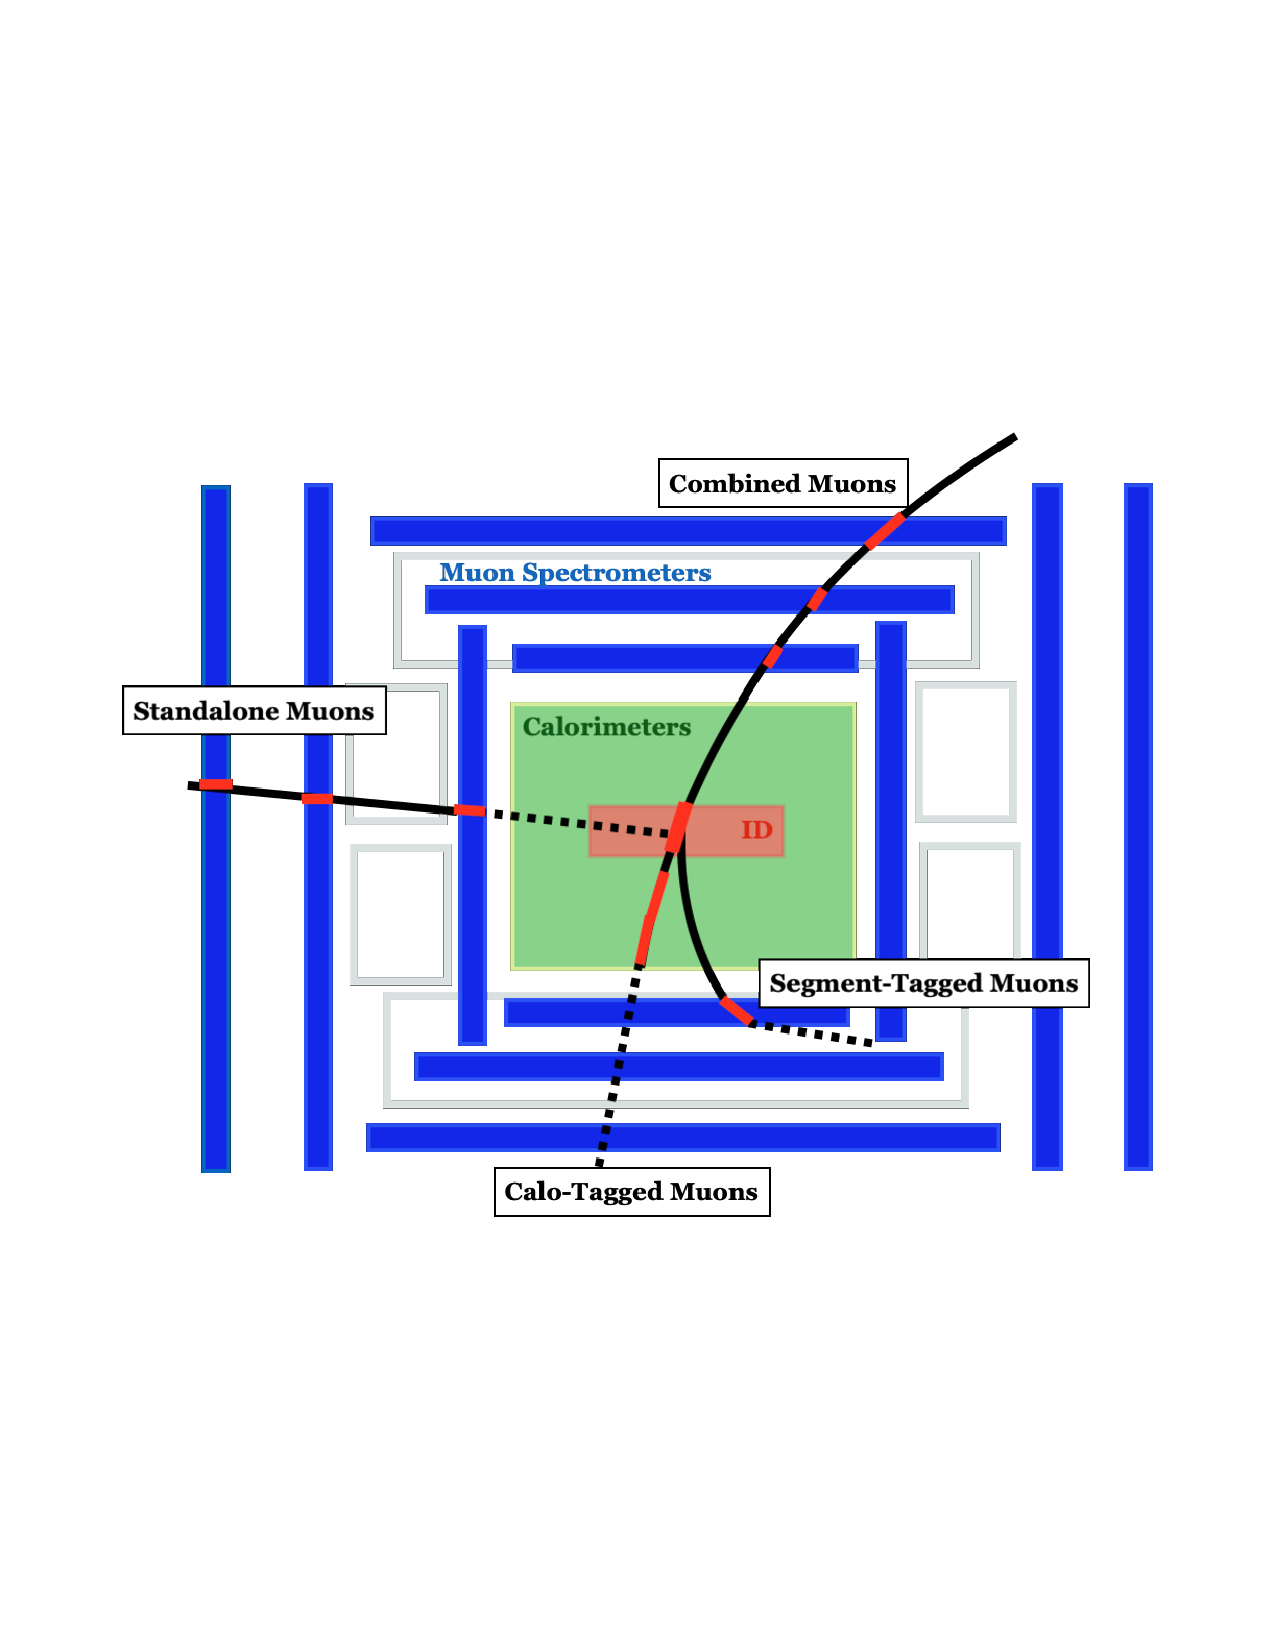
\includegraphics[width=.5\linewidth]{figures/LHC/MuonTypes.pdf}
    \caption{ Schematic of four different types of muons reconstructed using several layers of sub-detectors \cite{MuonReco}.\label{fig:MuonFig}}
\end{figure}

Similar to the electron reconstruction discussed in Section \ref{subsec:ParticleRecon_Elec}, reconstructed muons from the hard scatter are identified and isolated from the muons originating from secondary sources. Muon identification working points are developed by applying quality requirements in the simulated $t\bar{t}$ events where a $W$ from top-quark decay decays to a muon and a neutrino. The quality cuts require at least one-pixel hit, five SCT hits, less than three pixel or SCT holes, and at least $10\%$ of TRT hits to be included in the fit for the $0.1<\eta<0.9$ range with full TRT coverage \cite{MuonReco}. Three variables are used in muon identification; $q/p$ significance, which is defined as the ratio of muon's charge and momentum divided by the sum-quadrature of their uncertainties; $\rho^{'}$ defined as the absolute difference of transverse momentum measurements in the ID and MS divided by the combined track's $p_{T}$; and the normalized $\chi ^{2}$ of the combined track fit \cite{MuonReco}. 
Four identification \textit{working points}, Loose, Medium, Tight, and High-$p_{T}$ are defined for muons. The measurement uses a Loose identification point, which comprises all four types of muons and is developed for processes with four leptons in the final state  \cite{MuonReco}. 

To evaluate the total reconstruction efficiency of muons, $Z \rightarrow \mu\mu$ and $J/\psi \rightarrow \mu\mu$ events are used. The reconstruction efficiency in the region with ID coverage $|\eta|<2.5$ is obtained by using the tag-and-probe method, whereas, for $|\eta|>2.5$ region, it is estimated by evaluating SFs based on a double ratio of data and MC in $Z \rightarrow \mu\mu$ events \cite{MuonEffLargeEta}.

Analogous to electrons, muons are required to meet calo-based and ID-based isolation requirements. Muons in the measurement satisfy \textit{PflowLoose$\_$VarRad} isolation working point. Like in the case of electrons, systematic uncertainties on different scale factors for muon reconstruction, identification, isolation, and trigger efficiencies are propagated to the final cross-section measurement.

\subsection{Jet Reconstruction}
\label{subsec:ParticleRecon_Jets}

	\section{Future Upgrades}
\label{sec:FutureUpgrades}

\subsection{High Luminosity LHC}
\label{subsec:HLLHC}
The planned High Luminosity Large Hadron Collider (HL-LHC) is expected to operate starting mid-2029. The primary goals of HL-LHC are to collect large high-quality data statistics needed to study rare SM processes such as Higgs self-interaction, Higgs couplings to lighter particles, the longitudinal component of vector boson scattering, and to extend the BSM searches beyond the current reach of LHC. The HL-LHC upgrade aims to increase the center-of-mass energy of proton-proton collisions to $\sqrt{s}=14$ TeV and the instantaneous luminosity up to $\mathcal L = 7.5 \times 10^{34} cm^{-2}s^{-1}$ \cite{HLLHC}. Figure \ref{fig:HLLHC} shows the complete operation of LHC starting in 2011 to the planned decade-long HL-LHC program. 

\begin{figure}
    \centering
    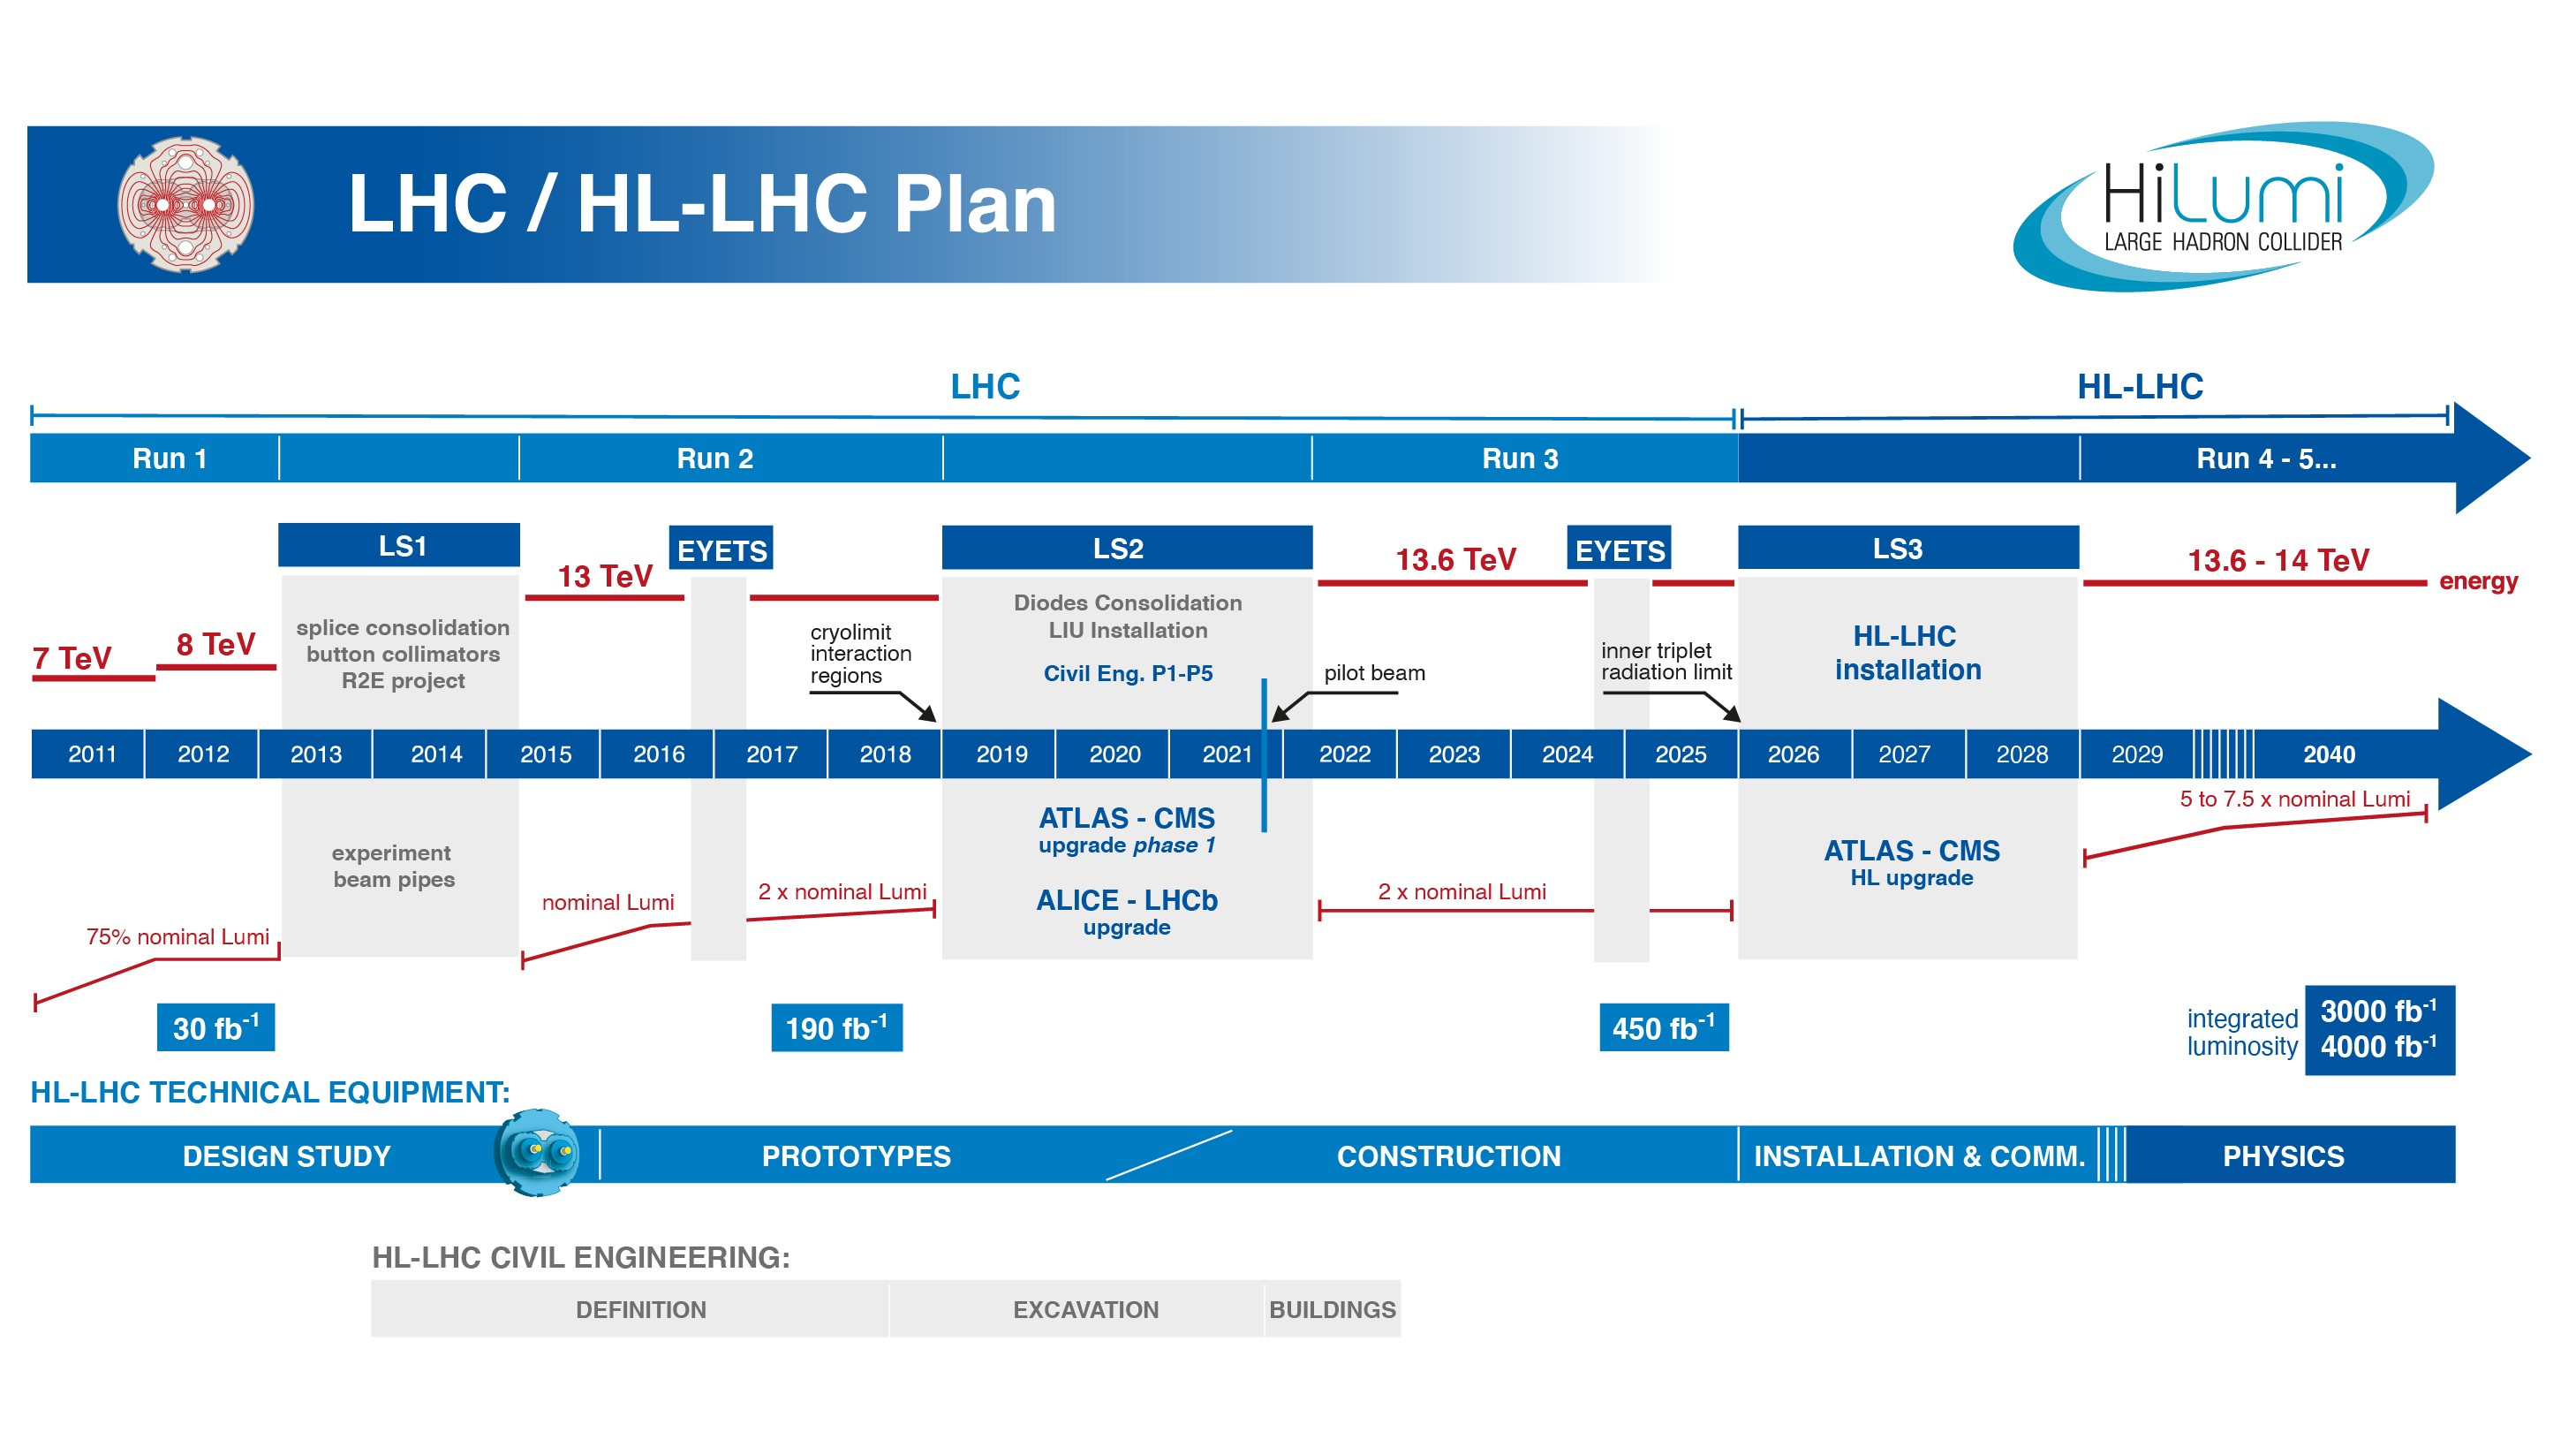
\includegraphics[width=.95\linewidth]{figures/LHC/HLLHCPlan.jpeg}
    \caption{ Timeline of LHC operation starting from 2011 to planned HL-LHC upgrade. Taken from \small{https://hilumilhc.web.cern.ch/content/hl-lhc-project}.\label{fig:HLLHC}}
\end{figure}
\normalsize

\subsection{ATLAS Upgrades}
\label{subsec:ATLASUpgrade}
At HL-LHC, about $200$ interactions per bunch crossing are expected, giving rise to several detector challenges, such as higher detector occupancy, harsher radiation conditions, and higher particle fluxes \cite{HLLHC}. The atlas detector will undergo a Phase-II upgrade to upgrade several sub-systems of ATLAS to meet the challenges of HL-LHC. The main upgrades include upgrading the muon system by adding new chambers in the inner barrel region, upgrading the trigger $\&$ data acquisition system to meet challenges from higher detector occupancy, and upgrading the electronics of several sub-systems. Additionally, a new High Granularity Timing Detector (HGTD) will also be inserted in the end-caps to supplement the tracking system and, most importantly replacement of the current ID with all Silicon Inner Tracking Detector (ITk) \cite{HLLHC}.

The ITk consists of Silicon pixel and strip detectors to increase granularity and radiation hardness with less material in the detector. Figure \ref{fig:ITKLayout} schematically shows the ITk layout with $5$ inner layers of pixel detector and four outer layers of strips detector. The tracking for ITk is extended in the forward region up to $|\eta| < 4.0$ region \cite{ITkStripsTDR}. 

\begin{figure}
    \centering
    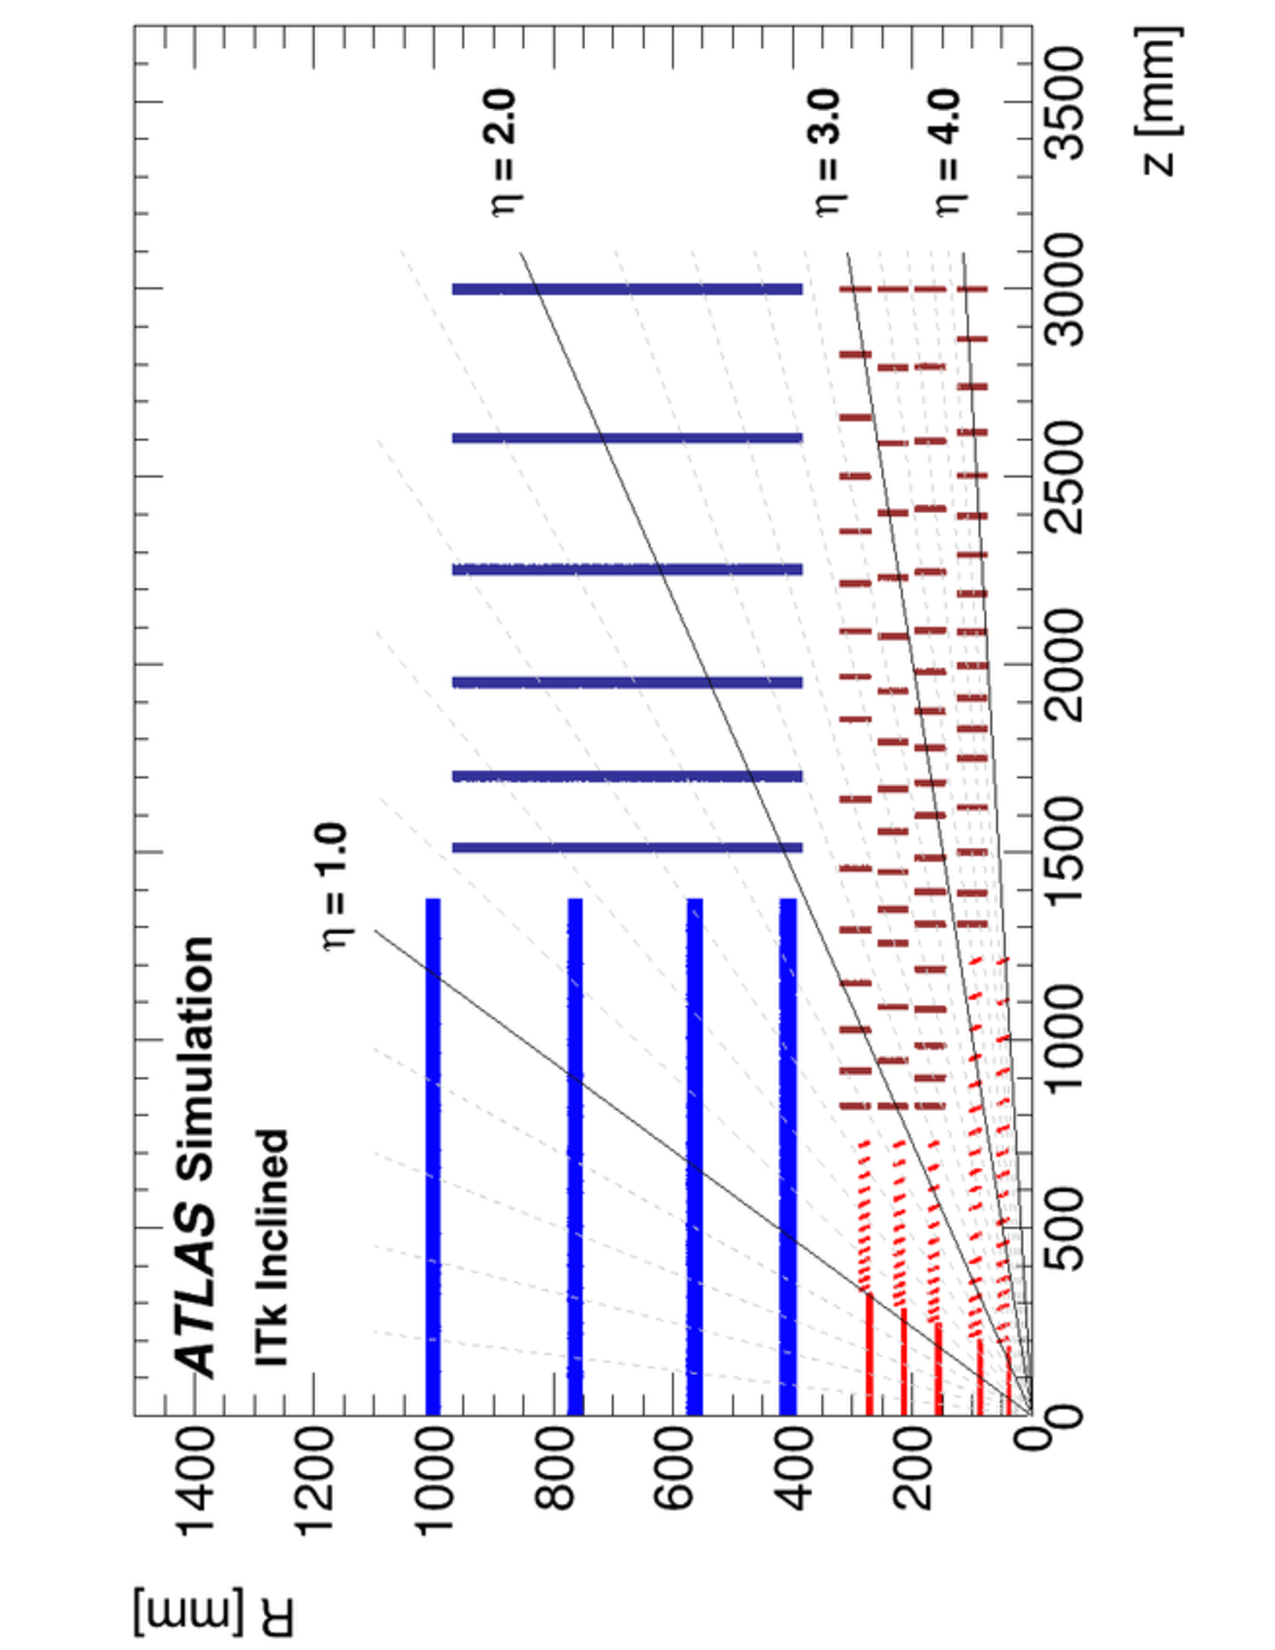
\includegraphics[angle=270,width=.95\linewidth]{figures/LHC/ITKLayout.pdf}
    \caption{ Schematic layout of ITK \cite{ITkPixelTDR}.\label{fig:ITKLayout}}
\end{figure}

More extensive statistics, extended tracking in the forward region, and the timing information from the HGTD HL-LHC program are highly beneficial to VBS $ZZjj$ measurements with extremely small cross-sections and two jets in the forward regions. 
\clearpage

\part {Analysis Overview}
\label{sec:AnalysisOverview}

\section{Goals}
\label{sec:Analysis_Goals}

The primary goal of this analysis is to measure the differential cross-section of $ZZ^*(\rightarrow 4\ell) jj$ processes as a function of several kinematic observables sensitive to the EWK production mode. The clean final state provides an invaluable avenue to study the rare electroweak production mode, which is experimentally accessible for the first time with LHC Run-2 statistics. The differential cross-sections are measured in a VBS-Enhanced region within a fiducial phase space that falls under the physical acceptance of the detector. For simpler re-interpretation in the future without ATLAS detector simulations, the differential cross-sections are measured at the particle-level using an unfolding technique, which removes the detector effects, such as limited efficiency and resolution. The measured cross-sections are then compared to the most precise SM predictions. As discussed in Section \ref{sec:EWKPheno}, the electroweak production of $ZZ^*(\rightarrow 4\ell) jj$ consists of contributions from VBS and is sensitive to possible BSM effects. Therefore, the unfolded differential cross-sections are used to constrain parameters of BSM physics, modifying the quartic self-interactions of the vector bosons as shown in Figure \ref{fig:ZZjjFeynmanDiag_EWk_b}.
	\section{Detector-Level Object Selection}
\label{sec:ObjReconstruction}

This section summarizes the detector-level selections applied to the three physics objects, electrons, muons, and jets used in the measurement. These kinematic requirements ensure that only high-quality physics objects relevant to the $ZZ^*(\rightarrow 4\ell) jj$ production are selected for the final measurement. Each physics object considered in the analysis is categorized as \textit{baseline} or \textit{signal}. Physics objects satisfying a set of kinematic selections or looser identification criteria are categorized as \textit{baseline}. In contrast, the baseline objects that pass either stricter kinematic selections or additional isolation and track-to-vertex association (TTVA) requirements are categorized as \textit{signal objects}.

\subsection{Electrons}
\label{subsec:ElecRecon}

Baseline electron objects are required to satisfy the kinematic selections of $\Pt~ > 7$ GeV and $|\eta| < 2.47$ and a loose likelihood identification working point of \textit{LHVeryLoose}. Some baseline electron candidates are reconstructed by matching the pile-up tracks to the calorimeter cluster deposit. A loose vertex association requirement of $|z_{0}\sin\theta| < 0.5 $ mm is applied to the baseline electron candidates to avoid these wrongfully reconstructed electrons. 

Signal electrons are required to pass a more stringent loose likelihood identification, \textit{LHLooseBL}, which requires at least one hit in the innermost layer of the pixel detector (IBL). The signal electrons are distinguished by tightening the impact parameter significance of the baseline electrons to $d_{0}/ \dZeroSig < 5$ and requiring an additional isolation working point identification of \textit{LooseVarRad} defined in Section \ref{subsec:ParticleRecon_Elec}. Table \ref{tab:Electron_RecoSel} summarizes the several kinematic selections imposed to define the baseline and signal electrons.

\begin{table}[!htbp]
    \centering
        \caption{Definition of the baseline and signal electrons.\label{tab:Electron_RecoSel}}
        \begin{tabular}{|| l || c | c ||}
        \hline
        Selection Category & \textbf{Baseline} & \textbf{Signal} \\
        \hline\hline
        Kinematic cuts & $p_{T} > 7$ GeV & $ p_{T} > 7$ GeV \\
                    & $|\eta| < 2.47$  &  $|\eta| < 2.47$\\
        \hline  
        Identification & LHVeryLoose & LHLooseBL \\
        \hline 
        Vertex Association & $|z_{0}\sin\theta| < 0.5$ mm & $|z_{0}\sin\theta|< 0.5$ mm\\
        \hline
        Isolation Working Point & $-$ & LooseVarRad\\
        \hline 
        Impact Parameter Significance & $-$ & $d_{0}/ \sigma_{d_{0}} < 5$ \\
        \hline
    \end{tabular}
\end{table}

\subsection{Muons}
\label{subsec:MuonRecon}
Baseline muons are required to satisfy $ |\eta| < 2.7 $, $p_{T} > 5$ GeV, a loose impact parameter requirements of $|z_{0}\sin\theta| < 0.5 $ mm, and \textit{Loose} identification working point. The signal muons are identified from the baseline muons by requiring additional isolation identification of \textit{PflowLooseVarRad} defined in Section~\ref{subsec:ParticleRecon_Muon} and tightening the TTVA requirements to $d_{0}/\sigma_{d_{0}} < 3$. Table \ref{tab:muon_baseline_signal} summarizes the baseline and signal muons selection requirements.

\begin{table}[!htbp]
    \centering
        \caption{Definition of the baseline and signal muons.\label{tab:muon_baseline_signal}}
        \begin{tabular}{|| l || c | c ||}
        \hline
        Selection Category & \textbf{Baseline} & \textbf{Signal} \\
        \hline\hline
        Kinematic cuts & $p_{T} > 5$ GeV & $p_{T} > 5$ GeV \\
                    & Calo-tagged $ p_{T} > 15$ GeV & Calo-tagged $ p_{T} > 15$ GeV \\
              & $|\eta| < 2.7$ & $|\eta| < 2.7$\\
        \hline
        Identification & Loose & Loose \\
        \hline 
        Vertex Association & $|z_{0}\sin\theta| < 0.5$ mm & $|z_{0}\sin\theta|< 0.5$ mm\\
        \hline
        Isolation Working Point & $-$ & PflowLooseVarRad\\
        \hline 
        Impact Parameter Significance & $-$ & $d_{0}/\sigma_{d_{0}} < 3$ \\
        \hline
    \end{tabular}
\end{table}

\subsection{Jets}
\label{subsec:JetRecon} 
As discussed in Section \ref{sec:EWKPheno}, the jets from the EWK $ZZ^*jj$ production are highly energetic; thus, reconstructed jets are required to have $p_{T} > 30$ GeV. The jet energy scale and resolution calibration discussed in Section \ref{subsec:ParticleRecon_Jets} is only valid for jets within $ |\eta| < 4.5 $ region. Therefore, the baseline jets are required to be in the $ |\eta| < 4.5 $ region. Baseline jets in $ |\eta| < 2.4 $ satisfying the \textit{Tight} working point of the \textit{Jet-vertex-tagger (JVT)} tool, and in $ |\eta| > 2.5 $ satisfying the \textit{Tight} working point of \textit{forward-jet-vertex-tagger (fJVT)} tool are classified as signal jets. Table \ref{tab:jets} summarizes the details of baseline and signal jets selection. 

A particular type of jets, the \textit{b-jets}, containing b-hadrons initiated from a b-quark, is also used for the background estimation. The b-jets reconstruction relies on multivariate analysis (MVA), utilizing the fact that b-hadrons have a long mean lifetime (about $1$ picosecond), leading to a displaced secondary vertex in the detectors. A tagger discussed in detail in Ref \cite{bTagging} with b-tagging efficiency of $77\%$ is used in the analysis to identify b-jets.

\begin{table}[!htbp]
    \centering
    \caption{Definition of the baseline and signal jets.\label{tab:jets}}
        \begin{tabular}{|| l || c | c ||}
        \hline
        Selection Category & \textbf{Baseline} & \textbf{Signal} \\
        \hline\hline
        Kinematic cuts & $\Pt~ > 30$ GeV & $\Pt~ > 30$ GeV \\
             & $|\eta| < 4.5$ & $|\eta| < 4.5$\\
        \hline
        Jet-Vertex-Tagger & $-$ & $ |\eta| < 2.4 $ JVT ("Tight")\\
                & $-$ & $|\eta| > 2.5 $ fJVT ("Tight")\\
        \hline
    \end{tabular}
\end{table}

\subsection{Overlap Removal}
\label{subsec:OR}

In order to avoid double-counting, an \textit{overlap removal} procedure is applied to remove physics objects reconstructed from the same detector signal. The measurement uses a lepton-favored overlap removal which selects leptons over jets. Overlap removal is an iterative process in which only objects surviving all previous steps are used in the subsequent steps. Table \ref{tab:overlap_removal} summarizes the overlap removal steps, where the $\Delta R$ is the angular separation between objects calculated using rapidity.

\begin{table}[!htbp]
    \centering
        \caption{Overlap removal used in the analysis. An object removed in one step does not enter into the subsequent step. \label{tab:overlap_removal}}
        \begin{tabular}{|| l || c | c ||}
        \hline
        Remove Object & Accept Object & Overlap Criteria \\
        \hline\hline
        Electron & Electron & Share a track or have overlapping calorimeter cluster.\\
                &       & Keep electron with higher $p_{T}$\\
        \hline
        Muon & Electron & Share ID track, and the muon is calo-tagged\\
        \hline
        Electron & Muon & Share ID track\\
        \hline
        Jet & Electron & $\Delta R_{e-jet} < 0.2$ \\
        \hline 
        Jet & Muon & $\Delta R_{\mu-jet} < 0.2/$ghost-associated and $N_{jet~tracks} < 3$\\
        \hline
    \end{tabular}
\end{table}
	\section{Trigger}
\label{sec:Trigger}

Due to the presence of four fully reconstructed leptons in the final state, the data events and detector-level MC events are preselected using a logical OR of different single and double-lepton triggers. The trigger menu varies according to the data-taking run periods to reflect the changes in the high-level trigger system, which are required to cope with increasing data rates. Additionally, trigger matching is required for the selected events. The trigger matching selects a subset of preselected events in which at least one lepton of the quadruplet is matched to one of the fired triggers. Table \ref{tab:Trigger} shows the trigger menu used by the analysis per different data periods using either electrons, muons, or mixed electron-muon triggers.

\begin{table}
    \centering
    \begin{tabular}{| l | c | c |}
    \hline 
    Period & Leptons & Triggers \\
    \hline
    \multirow{10}{*} {2015} & \multirow{4}{*} {Electron} &  HLT$\_$e24$\_$lhmedium$\_$L1EM20VH  \\
                        &          &  HLT$\_$e60$\_$lhmedium \\
                        &    & HLT$\_$e120$\_$lhloose \\
                        & &  HLT$\_$2e12$\_$lhvloose$\_$L12EM10VH\\\cline{2-3}

                        & \multirow{4}{*} {Muon} & HLT$\_$mu20$\_$iloose$\_$L1MU15 \\
                        & & HLT$\_$mu50 \\
                        & & HLT$\_$2mu10 \\
                        & & HLT$\_$mu18$\_$mu8noL1 \\\cline{2-3}
                        & \multirow{2}{*}{Mixed} & HLT$\_$e7$\_$lhmedium$\_$mu24 \\
                        & & HLT$\_$e17$\_$lhloose$\_$mu14 \\
    \hline
    \multirow{10}{*} {2016} & \multirow{4}{*} {Electron} & HLT$\_$e26$\_$lhtight$\_$nod0$\_$ivarloose \\
                        &          & HLT$\_$e60$\_$lhmedium$\_$nod0 \\
                        & & HLT$\_$e140$\_$lhloose$\_$nod0\\
                        & &  HLT$\_$2e17$\_$lhvloose$\_$nod0 \\\cline{2-3}
                        & \multirow{4}{*} {Muon} & HLT$\_$mu26$\_$ivarmedium \\
                        & & HLT$\_$mu50 \\
                        & & HLT$\_$2mu14 \\
                        & & HLT$\_$mu22$\_$mu8noL1 \\\cline{2-3}
                        & \multirow{2}{*}{Mixed} & HLT$\_$e7$\_$lhmedium$\_$nod0$\_$mu24  \\
                        & & HLT$\_$e17$\_$lhloose$\_$nod0$\_$mu14 \\
    \hline
    \multirow{10}{*} {2017} & \multirow{4}{*} {Electron} &  HLT$\_$e26$\_$lhtight$\_$nod0$\_$ivarloose \\
                        & &  HLT$\_$e60$\_$lhmedium$\_$nod0 \\
                        & & HLT$\_$e140$\_$lhloose$\_$nod0 \\
                        &          & HLT$\_$2e24$\_$lhvloose$\_$nod0 \\\cline{2-3}
                        & \multirow{4}{*} {Muon} & HLT$\_$mu26$\_$ivarmedium \\
                        & & HLT$\_$mu50 \\
                        & & HLT$\_$2mu14 \\
                        & & HLT$\_$mu22$\_$mu8noL1  \\\cline{2-3}
                        & \multirow{2}{*}{Mixed} &  HLT$\_$e17$\_$lhloose$\_$nod0$\_$mu14  \\
                        & & HLT$\_$e26$\_$lhmedium$\_$nod0$\_$mu8noL1 \\
    \hline
    \multirow{10}{*} {2018} & \multirow{4}{*} {Electron} & HLT$\_$e26$\_$lhtight$\_$nod0$\_$ivarloose \\
                        &          & HLT$\_$e60$\_$lhmedium$\_$nod0  \\
                        &          & HLT$\_$e140$\_$lhloose$\_$nod0 \\
                        &          &  HLT$\_$2e24$\_$lhvloose$\_$nod0 \\\cline{2-3}
                        & \multirow{4}{*} {Muon} & HLT$\_$mu26$\_$ivarmedium \\
                        & & HLT$\_$mu50  \\
                        & & HLT$\_$2mu14 \\
                        & &  HLT$\_$mu22$\_$mu8noL1 \\\cline{2-3}
                        & \multirow{2}{*}{Mixed} & HLT$\_$e17$\_$lhloose$\_$nod0$\_$mu14 \\
                        & &  HLT$\_$e26$\_$lhmedium$\_$nod0$\_$mu8noL1  \\
    \hline
    \end{tabular}
    \caption{Trigger menu used in the analysis for event preselection \label{tab:Trigger}}
\end{table}

The trigger efficiency of MC is defined as a ratio of events passing the logical OR selection of the triggers to the number of events passing reconstruction level pre-trigger selection. The trigger efficiency for MC events could differ from that for the data. Thus, trigger efficiency scale factors are applied to MC events to account for the differences. The scale factors are defined as a fraction of trigger efficiency for MC to that of data and retrieved from the ATLAS supported tool \textit{TrigGlobalEffciencyCorrectionTool}\footnote{https://gitlab.cern.ch/atlas/athena/tree/21.2/Trigger/TrigAnalysis/TrigGlobalEfficiencyCorrection}.

Figure \ref{fig:Trigger} shows the efficiency of trigger selection in events with a signal quadruplet and a dijet as a function of $m_{4\ell}$. The efficiency is almost $100\%$ over the whole spectrum. The black distribution shows the total detector-level preselected events, the red distribution shows events passing at least one trigger requirement, and the blue distribution shows events passing both trigger and matching requirements. 
\begin{figure}
    \centering
    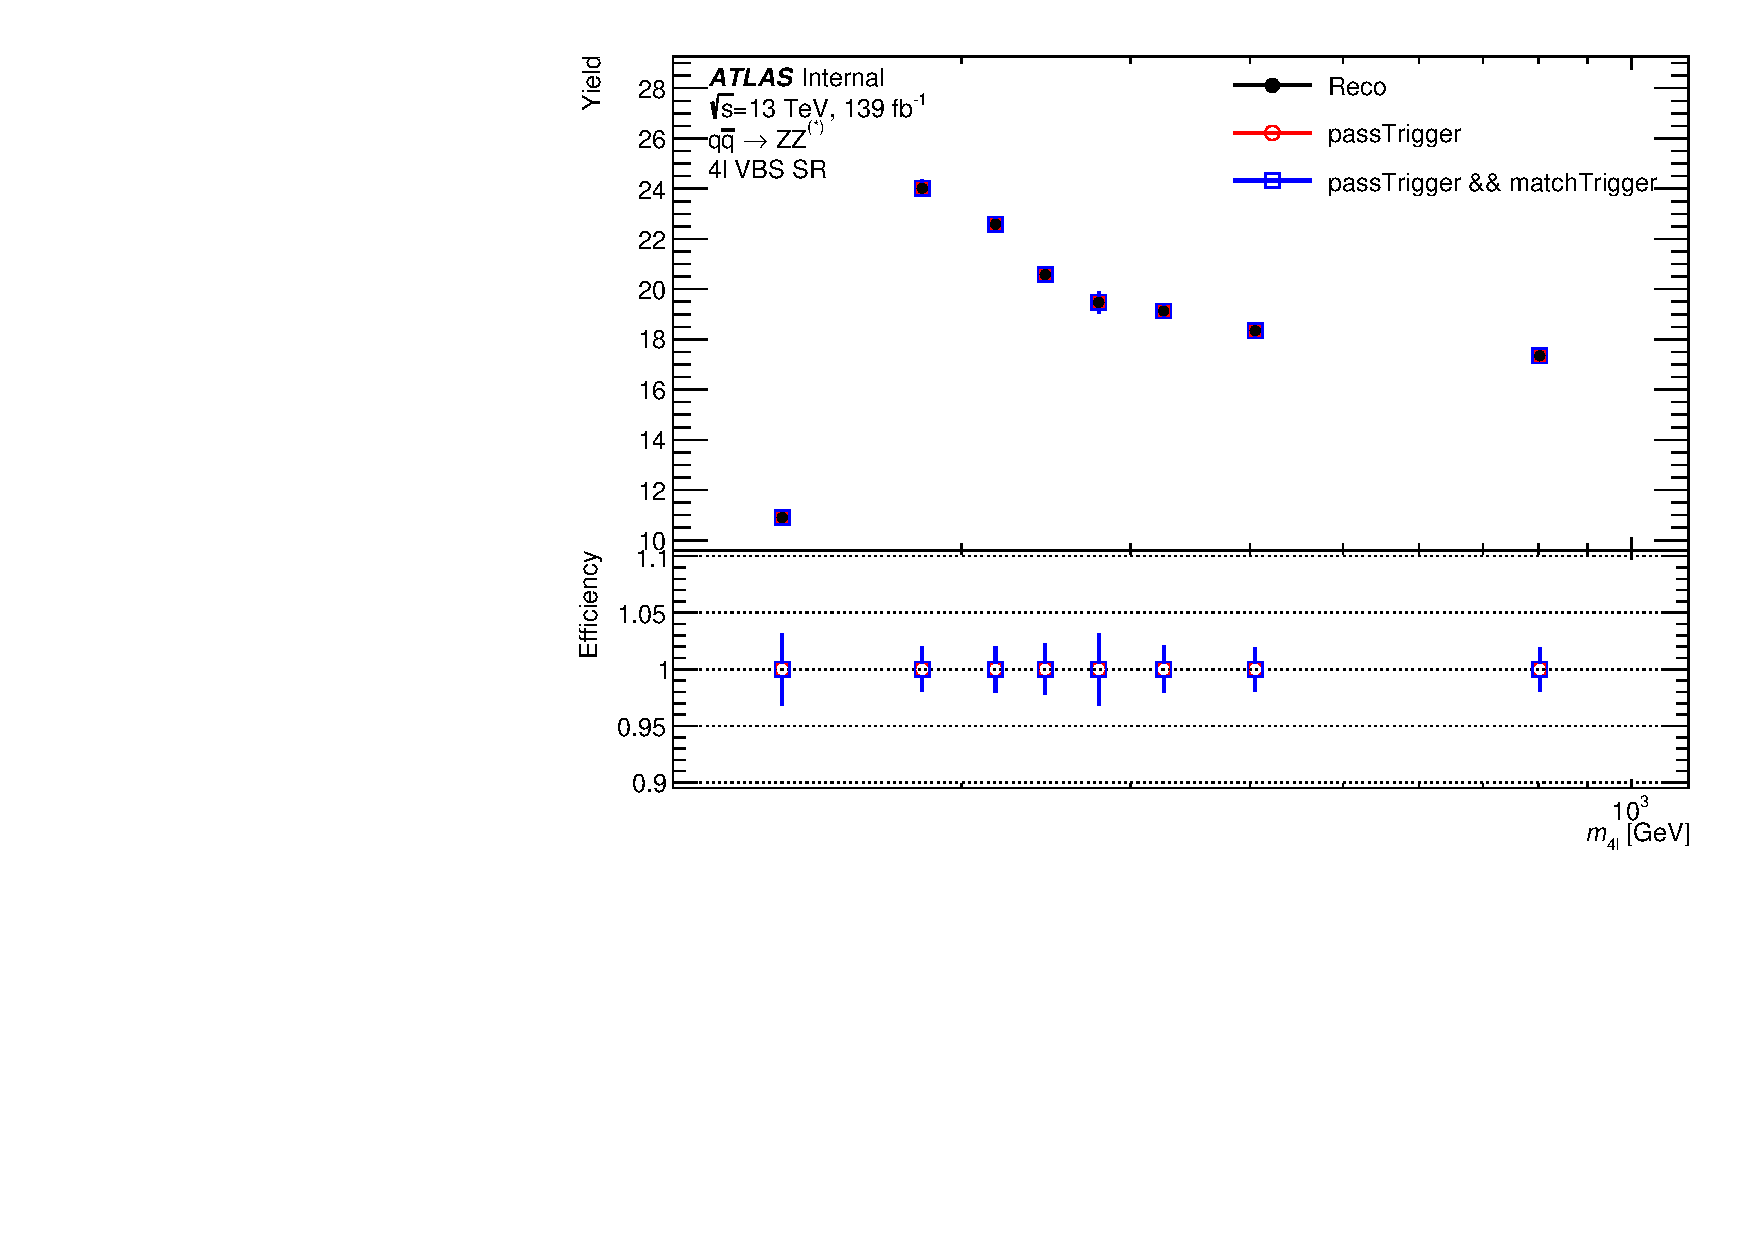
\includegraphics[width=.8\linewidth]{figures/AnalysisOverview/TriggerEfficiency.pdf}
    \caption{ Trigger efficiency as a function of $m_{4\ell}$.\label{fig:Trigger}}
\end{figure}
	\section{Event Selection}
\label{sec:EventSel}

A $ZZjj$ event at the detector level consists of a lepton quadruplet formed from SF-OC baseline-lepton pairs and a dijet, passing similar selections as the fiducial level defined in section \ref{sec:FidSel}. The leading and sub-leading leptons are required to satisfy $p_{T} > 20$ GeV to ensure a high trigger efficiency. From the leptons passing these requirements, at least two SF-OC lepton pairs with $\Delta R > 0.05$ and $m_{\ell\ell} > 5$ GeV are formed. A quadruplet is formed from the two SF-OC lepton pairs whose invariant masses are closest and next closest to the mass of the Z-boson ($m_{Z}$). Similar to the fiducial level selection, the lepton pair with the highest value of absolute rapidity is identified as the leading pair. The quadruplets with all four leptons passing the signal lepton criteria of the TTVA and isolation are the \textit{signal quadruplet} defining the signal region. While on the contrary, the quadruplets where one lepton fails either isolation or TTVA requirement used in the fake background estimation are the \textit{not-signal quadruplets}. 

A dijet in an event is selected by requiring two signal jets defined in section \ref{subsec:JetRecon} from the opposite side of the detector i.e., $\eta_{lead~jet} \times \eta_{sub-leading~jet} < 0)$. To maximize the probability of selecting an event from EWK $ZZjj$ production, a requirement of significant rapidity difference between the jets of $\Delta Y_{jj}> 2 $ and a large invariant mass of $m_{jj} > 300 $ GeV are imposed on the dijet selection. Table \ref{tab:EventSelection} summarizes all selections applied to select  $ZZjj$ detector-level events.


\begin{table}[!htb]
	\centering
		\caption{Details of event selection.\label{tab:EventSelection}}
		\begin{tabular}{|| l || c | c ||}
		\hline
		Event Selection 		& Cut 					& Requirement														\\
		\hline\hline
		Event  				& Trigger 					&  Fire at least one lepton trigger										\\
		Preselection         		& Vertex				 	& At least one vertex with $2$ or more tracks								\\
		\hline  
		 			& Lepton Kinematics 		& $p_{T}~ > 20$ GeV for two leading leptons						\\
					& Lepton Separation 		& $\Delta R_{ij} > 0.05$ between leptons in quadruplet		\\
		Quadruplet	& Pair Requirement 			& Two SF-OC lepton pairs											\\
		Selection	&						& $m_{\ell\ell} > 5$ GeV									\\
					& Minimal $\Delta m_{Z}$ 	& quadruplet with smallest $|m_{12}	- m_{Z} | + |m_{34}	- m_{Z} |$\\
					&						& Leading Pair: pair with highest $|y_{ij}|$						\\
					& ZZ Mass				& $m_{4\ell} > 130 $ GeV											\\
		\hline  
		Quadruplet 			& Signal Quadruplet			& Quadruplet with all \textbf{signal leptons}							\\
		Categorisation			& Not-Signal Quadruplet 		& Quadruplet with $\geq 1$ \textbf{baseline-not-signal lepton}			\\
		\hline  
		 			& Different Detector Sides		& $\eta_{lead~jet} \times \eta_{sub-leading~jet} < 0 $			\\
		Dijet		& Rapidity Separation 		& $	\Delta Y_{jj}> 2 $												\\
		Selection	& Leading Jet $p_{T}$ 	& 	$p_{T,~leading~jet} > 40$ GeV				\\
					& Dijet Mass 				& $m_{jj} > 300 $ GeV													\\
					& Dijet 		& Both jets required to pass either JVT or FJVT 							\\
		\hline  
							
		Event				& VBS-Enhanced Region 		& signal quadruplet $\&$ dijet and centrality ($\zeta) < 0.4 $				\\
		Categorisation			& VBS-Suppressed Region 	& signal quadruplet $\&$ dijet and centrality ($\zeta) > 0.4$				\\
		
		\hline
	\end{tabular}
\end{table}

Figure \ref{fig:EventDisplayZZjj} illustrates a signature of two $Z$-bosons production in an association of two jets. The event display corresponds to an event recorded during Run Number $340368$ of the 2017 data-taking period. The two light-yellow cones on two opposite sides of the detector with a large rapidity gap represent the reconstructed dijet of the event with $m_{jj} = 2228$ GeV. In this event, one of the SF-OC lepton pairs decays to  $e^+e^-$ ($Z\rightarrow e^+e^-$), and the other decays into $\mu^+\mu^-$ ($Z\rightarrow \mu^+\mu^-$).

\begin{figure}
\centering
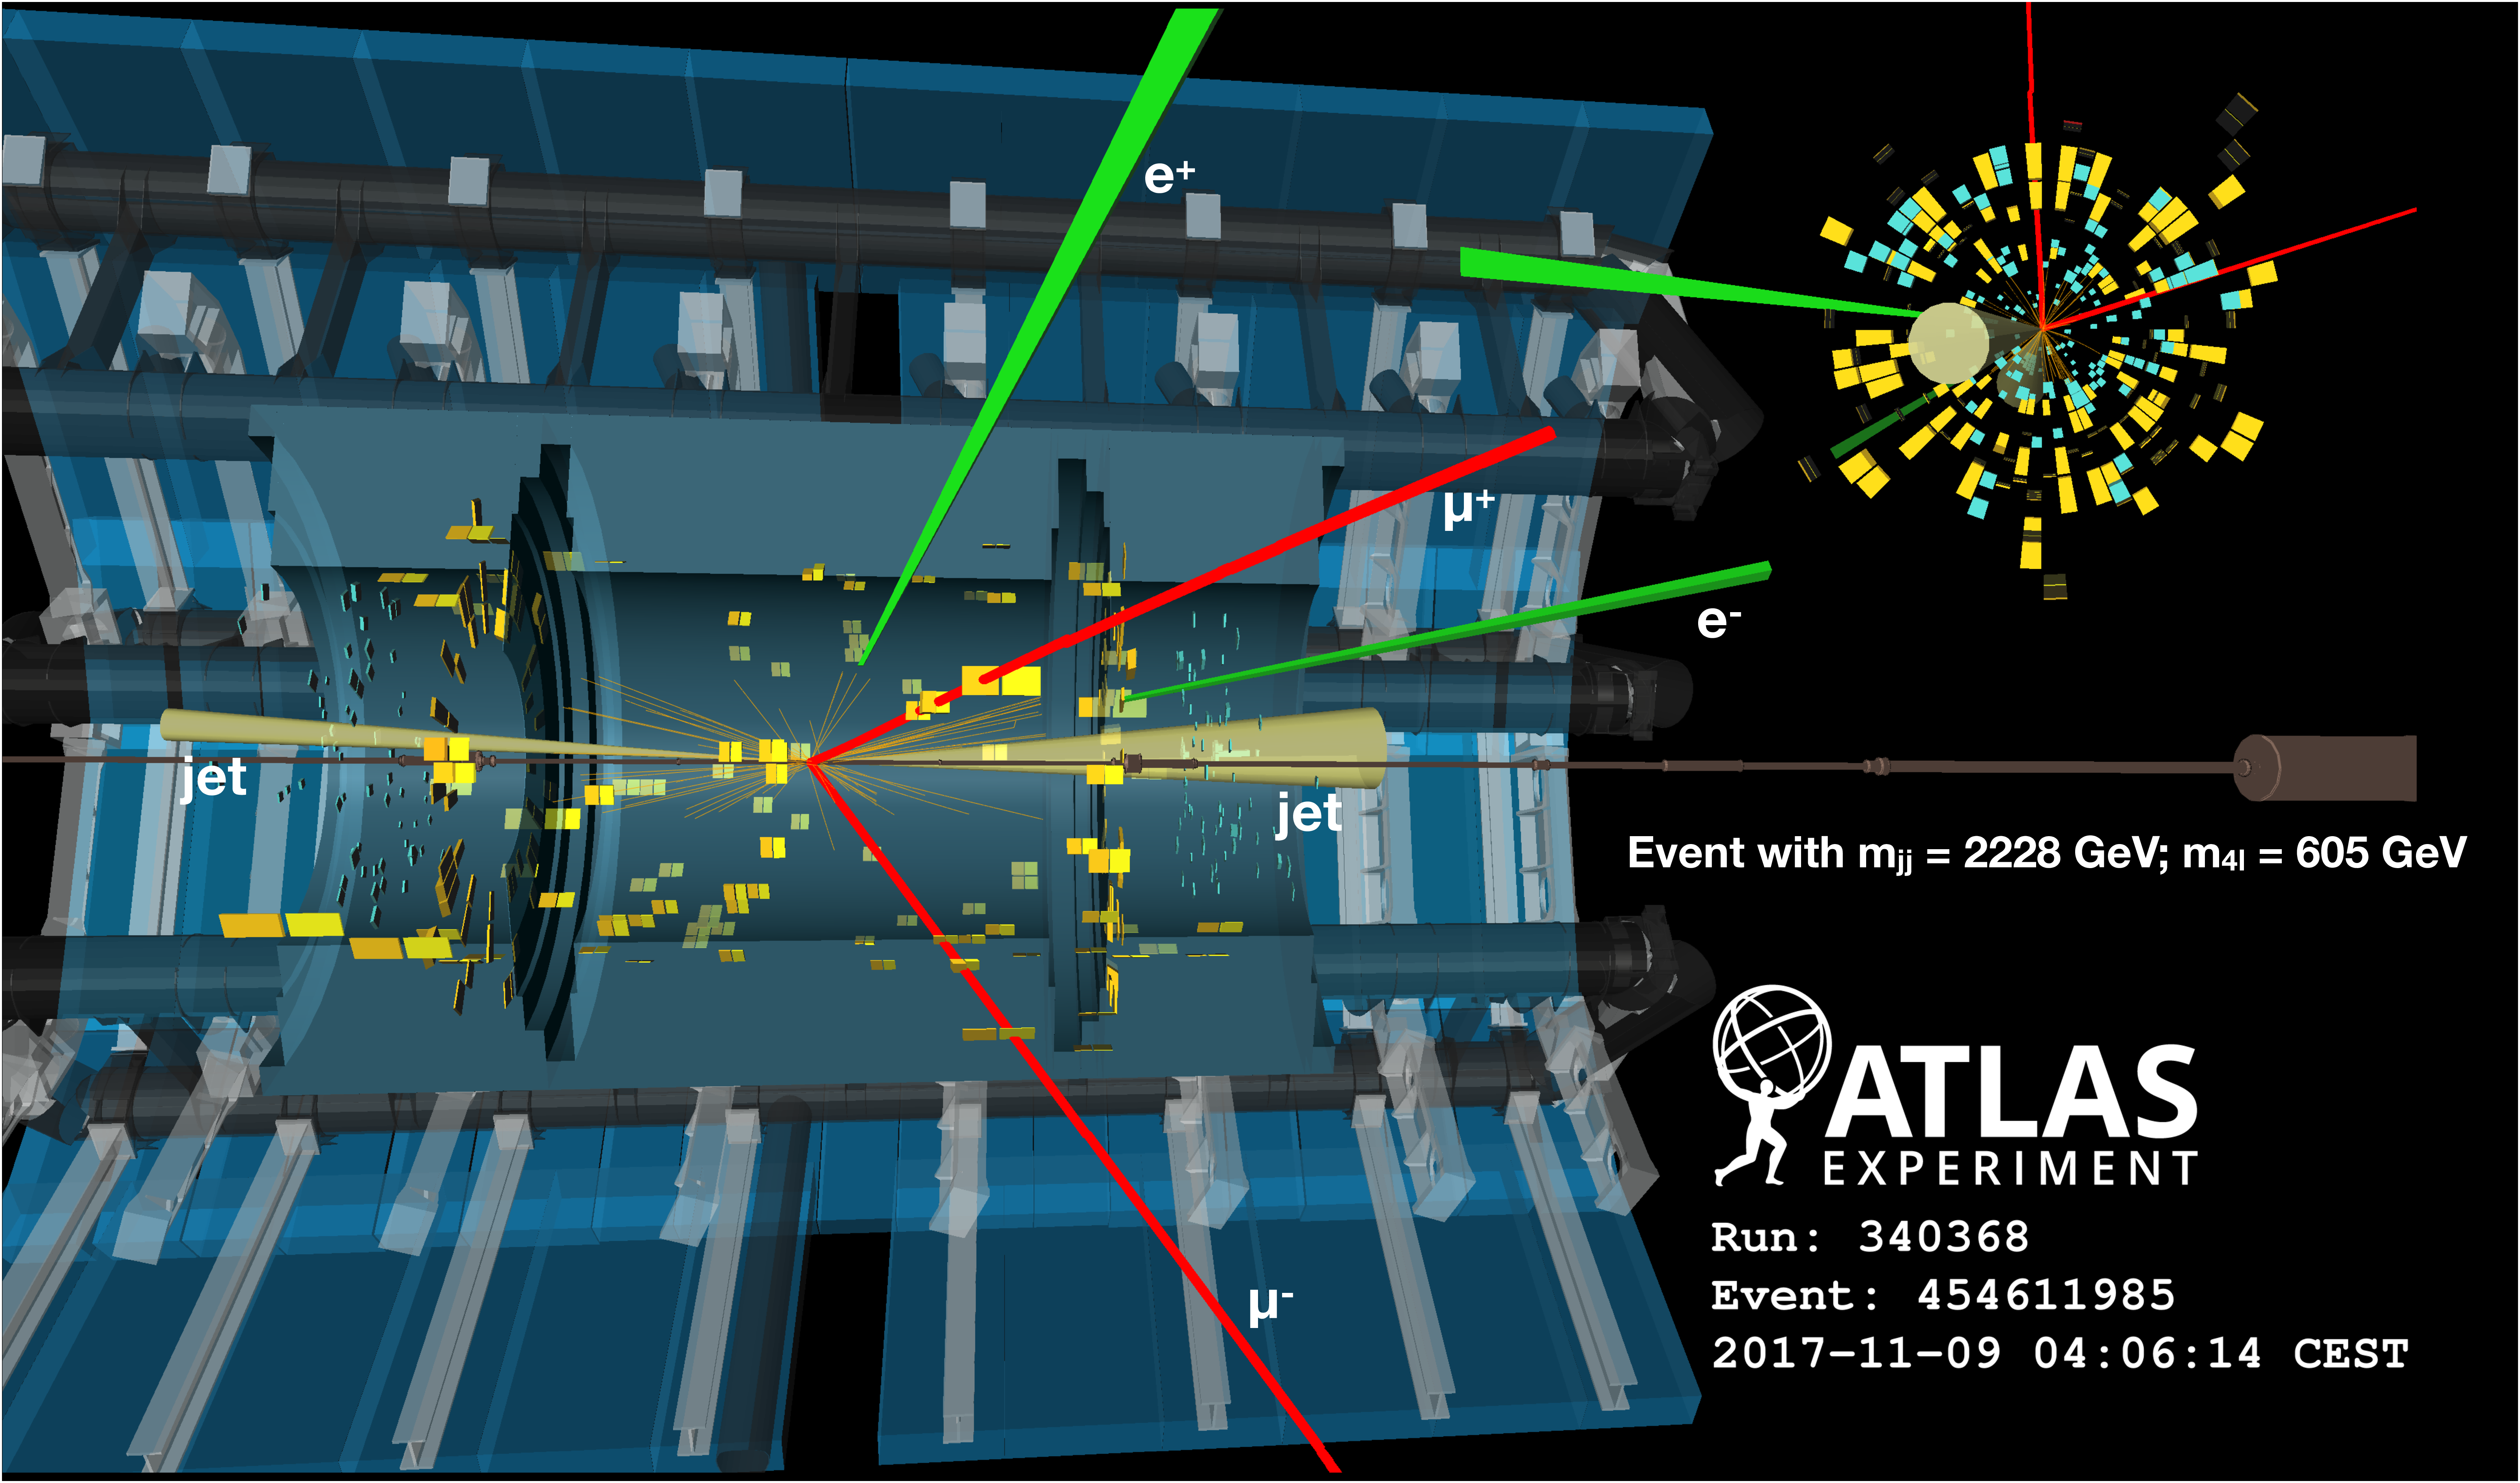
\includegraphics[width=.9\linewidth]{figures/AnalysisOverview/ZZjjEventDisplay.png}  
\caption{Event display of a candidate $pp \rightarrow ZZjj \rightarrow e^+e^-\mu^+\mu^- jj $ recorded by the ATLAS experiment in Run-$2$ $2017$ data-taking period. The invariant mass of the reconstructed four leptons is $m_{4\ell} = 605$ GeV, and that of the reconstructed di-jet is $m_{jj} = 2228$ GeV. The large rapidity separation between the two jet cones (light yellow) on the opposite sides of the ATLAS detector and centrally produced two $Z$ bosons defines the characteristic feature of the EWK production of ZZjj \label{fig:EventDisplayZZjj} \cite{ATLASZZjj}.}
\end{figure}
	\section{Phase Space Definition}
\label{sec:FidSel}

The unfolded differential cross-sections are measured in a phase space within the acceptance of the detector. This section summarizes the selections defining the fiducial phase space of the analysis.

\subsection{Fiducial Volume}
\label{subsec:FidVol} 

The fiducial phase space consists of $pp\rightarrow ZZ ( \rightarrow 4\ell) jj$ $[\ell = e,~\mu]$ events with four centrally produced prompt-leptons and two jets with significant rapidity separation as motivated by Section \ref{sec:EWKPheno}. The fiducial phase space does not contain any leptons from tau decays. Both fiducial-level electrons and muons are required to be dressed. The dressing procedure accounts for the energy losses of leptons through photon emissions via bremsstrahlung. Dressed leptons are constructed by adding the four-momenta of nearby photons within the lepton's small $\Delta R < 0.1$ cone. 

Several kinematic cuts summarized in Table \ref{tab:FidObjectCut} are applied individually to the muons, electrons, and jets to ensure the selected objects fall within detector acceptance before defining the events. Motivated by the discussion of physics object reconstruction in Section \ref{sec:ParticleReconstruction}, each electron is required to have $p_{T} > 7$ GeV and $|\eta| < 2.47$, whereas the muons satisfy $p_{T} > 5$ GeV and $|\eta| < 2.7$. Event quadruplets are formed by requiring two SF-OC lepton pairs, with leading and sub-leading lepton $p_{T}>20$ GeV and angular separation between any two leptons to satisfy $\Delta R > 0.05$. Additionally, the invariant mass of any SF-OC lepton pair is required to satisfy $m_{\ell \ell } > 5$ GeV to suppress the contamination from lower resonance backgrounds. Based on these requirements, the quadruplets can be of the following three types:

\begin{itemize}
\item{$4e$: events with two $e^{+}e^{-}$ pairs.}
\item{$4\mu$: events with two $\mu^{+}\mu^{-}$ pairs.}
\item{$2e2\mu$ or $2\mu2e$: events where one of the pair is $e^{+}e^{-}$ and other is $\mu^{+}\mu^{-}$}
\end{itemize}

In any event with more than two SF-OC lepton pairs, the quadruplet is formed by choosing the two pairs that minimize the distance to the $Z$ resonance pole. Once the quadruplet is formed, the leading-lepton pair is defined as the one with a higher absolute rapidity value, i.e., $|y_{ij}|$. Finally, an additional criterion on the invariant mass of the quadruplet of $m_{4\ell} > 130$ GeV is imposed. 

Similarly, the event dijet is constructed from the two leading jets with the opposite sign of pseudo-rapidity ($\eta$) to imitate the detector-level VBS dijet production, where jets are reconstructed on the opposite side of the detector. The jets are required to satisfy $|n| < 4.5$, $p_{T,~leading~jet} > 40$ GeV, and $p_{T,~sub-leading~jet} > 30$ GeV. The dijet is required to have a large rapidity separation of $|\Delta y_{jj}| > 2$ and high invariant mass of $m_{jj} > 300$ GeV to resemble dijet produced in electroweak $ZZ (\rightarrow 4 \ell) jj$ production. Table \ref{tab:QuadDijetFidCut} summarizes the requirements to select the quadruplet and the dijet in an event.

\begin{table}[ht]
    \centering
    \caption{Details of the kinematic pre-selection applied to the baseline electrons, muons, and jets. The required kinematic cuts are applied to the dressed leptons.
    \label{tab:FidObjectCut}}
    \begin{tabular}{|| l || c | c | c ||}
        \hline
        Selections      & Electrons             &       Muons        &          Jets            \\
        \hline\hline
        $\Pt~$          & $> 7$ GeV             &       $ >5$ GeV    &      $>30$GeV        \\
        \hline 
        $|\eta|$            &  $< 2.47  $           &       $ < 2.7 $        &      $ < 4.5$            \\
        \hline
    \end{tabular}
\end{table}             
    
\begin{table}[ht]
    \caption{Details of the selections applied to form a quadruplet and a dijet selection in the fiducial volume. 
    \label{tab:QuadDijetFidCut}}
    \begin{tabular}{|| l || c ||}
        \hline
        Selections              &           Cut \\
        \hline\hline
        Lepton Kinematics       & $P_{T,~leading~lepton} > 20 $ GeV\\
                                & $P_{T,~sub-leading~lepton} > 20 $ GeV\\
        \hline 
        Pair Requirement        & $\Delta R_{\ell i,\ell     j} > 0.05 $\\
                                & SF-OC with $\mll > 5$ GeV\\
        \hline
        Quadruplet Requirement  & $2$ pair candidates with smallest $|\mOneTwo  - m_{Z} | + |\mThreeFour    - m_{Z} |$  \\
                                & Leading pair: pair with highest $|y_{ij}|$\\
                                & Sub-leading pair: pair with lowest $|y_{ij}|$\\
                                & $\mFourL > 130 $ GeV\\
        \hline
        Di-jet Requirement      & $p_{T,~leading~jet} > 40$ GeV \\
                                & $|\Delta y_{jj}| > 2 $ \\ 
                                & $m_{jj} > 300$ GeV    \\
        \hline
    \end{tabular}
\end{table}

\subsection{Signal Region}
\label{subsec:SignalRegion}
The signal region of the analysis is defined based on the centrality ($\zeta$) of the di-$Z$boson production in an event. Centrality depends on the rapidity of the quadruplet and the rapidity of the dijet as:
\begin{equation}
    \zeta~=~\frac{|y_{quadruplet}~-~ 0.5*(y_{leading~jet}~+~y_{sub-leading~jet})| }{|y_{leading~jet}~-~y_{sub-leading~jet}|}
    \label{eq:centr}
\end{equation}

Figure \ref{fig:centrality_a} shows the predicted MC distribution of centrality for the three main production modes of $ZZ(\rightarrow 4 \ell)jj$. The significance of the EWK component over the inclusive parton initiated and $gg$-loop initiated QCD production is defined as, 
\begin{equation}
    s=\frac{N_{EWK}}{\sqrt{N_{QCD}^{(qq)}+N_{QCD}^{(gg)}}}
    \label{eqn:EWKSignificance}
\end{equation}
where $N_{EWK}$, $N_{QCD}^{qq}$ and $N_{QCD}^{gg}$ are the numbers of events from electroweak, parton initiated QCD and gluon-loop initiated QCD productions, respectively. The chosen cut value on the centrality maximizes the EWK significance while maintaining a good selection efficiency of EWK events. Figure in \ref{fig:centrality_b} shows the efficiency and significance for various cut values of centrality.  

A VBS-enhanced signal region is defined based on events with a quadruplet, a dijet, and $\zeta<0.4$. The low value of the centrality and the requirements for a signal dijet ensures that the events in this signal region originate in a more significant fraction from the electroweak production of $ZZ (\rightarrow 4 \ell) jj$. A VBS Suppressed control region is also defined based on events with a quadruplet, a dijet, and $\zeta>0.4$. These events mainly originate from the QCD production of $ZZ (\rightarrow 4 \ell) jj$ and are used to optimize the analysis strategies.

\begin{figure}[ht]
\begin{subfigure}{.48\textwidth}
  \centering
  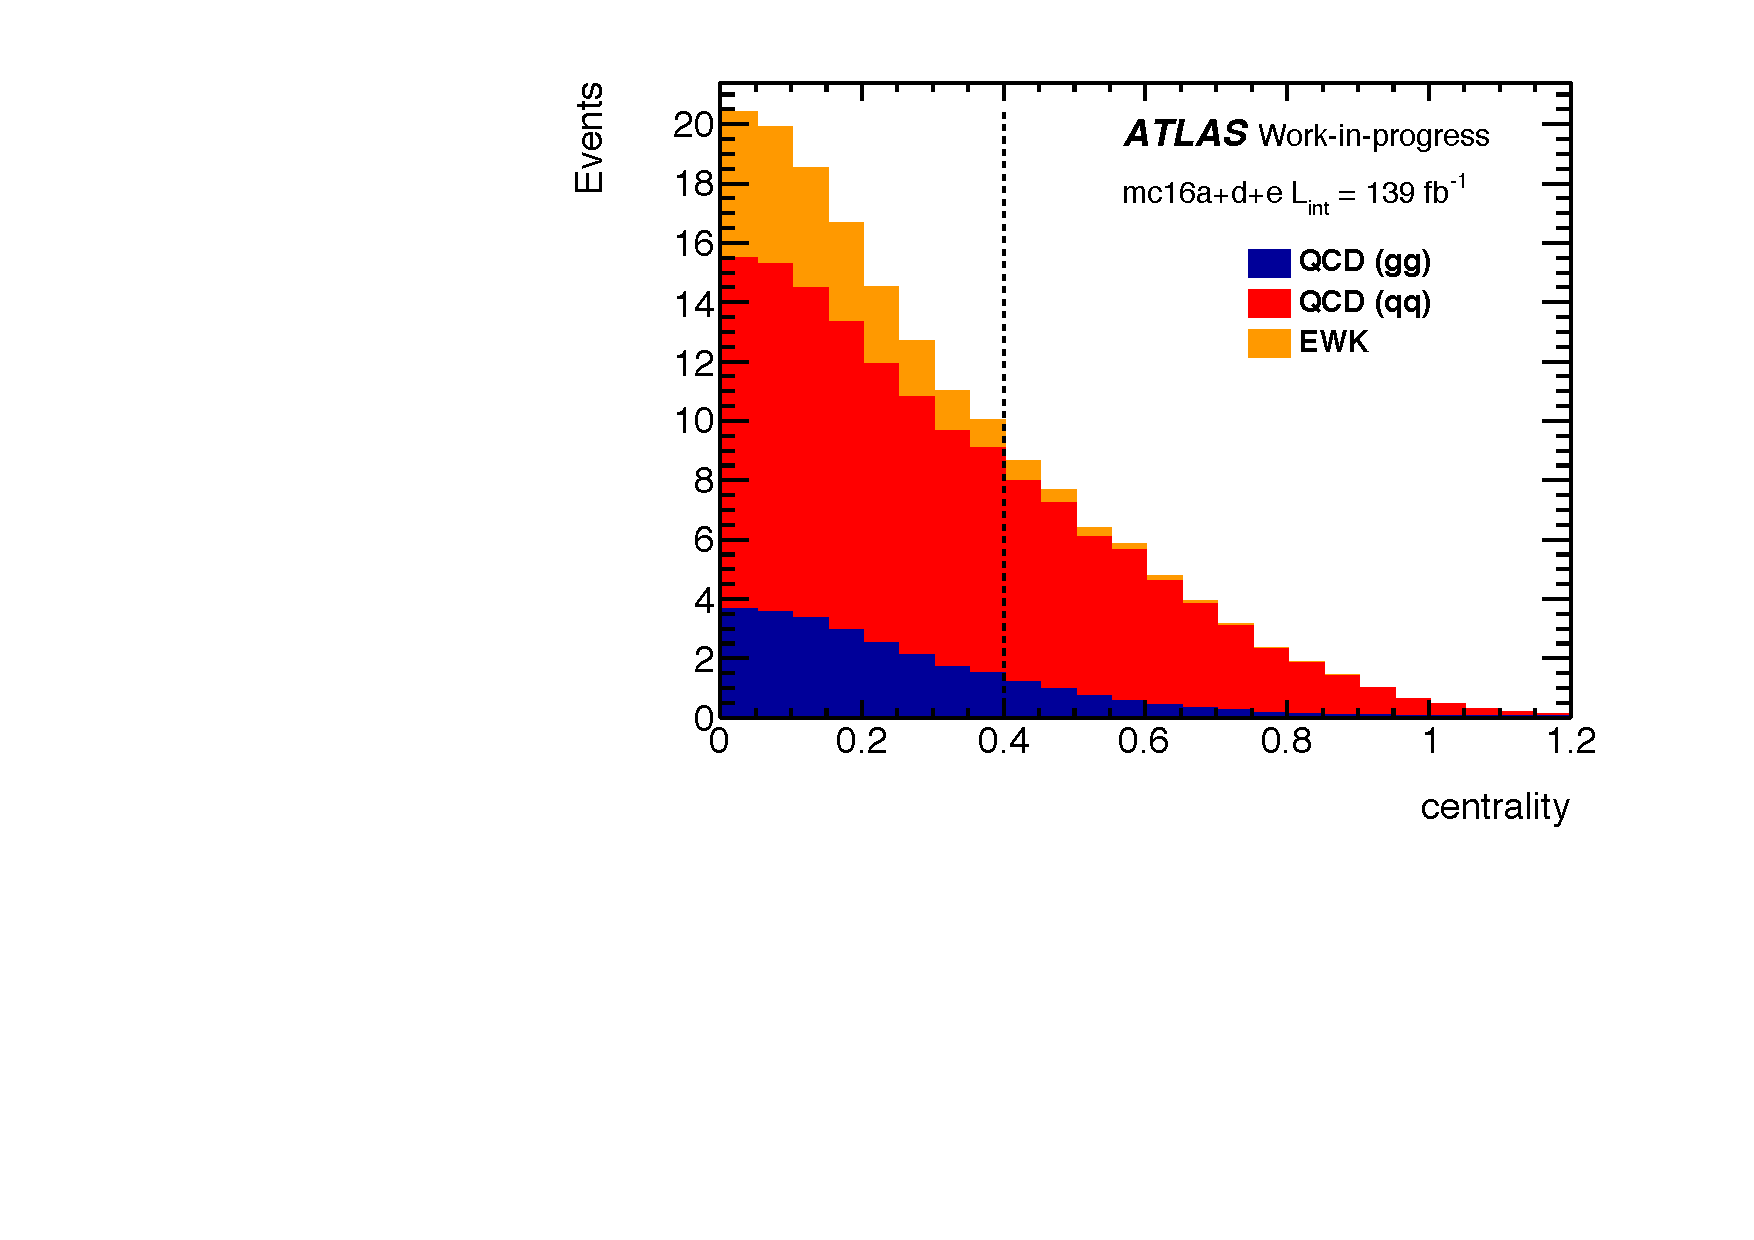
\includegraphics[width=.95\linewidth]{figures/AnalysisOverview/centrality_Dist.pdf}  
  \caption{Yields of EWK and QCD production.}
  \label{fig:centrality_a}
\end{subfigure}
\begin{subfigure}{.48\textwidth}
  \centering
  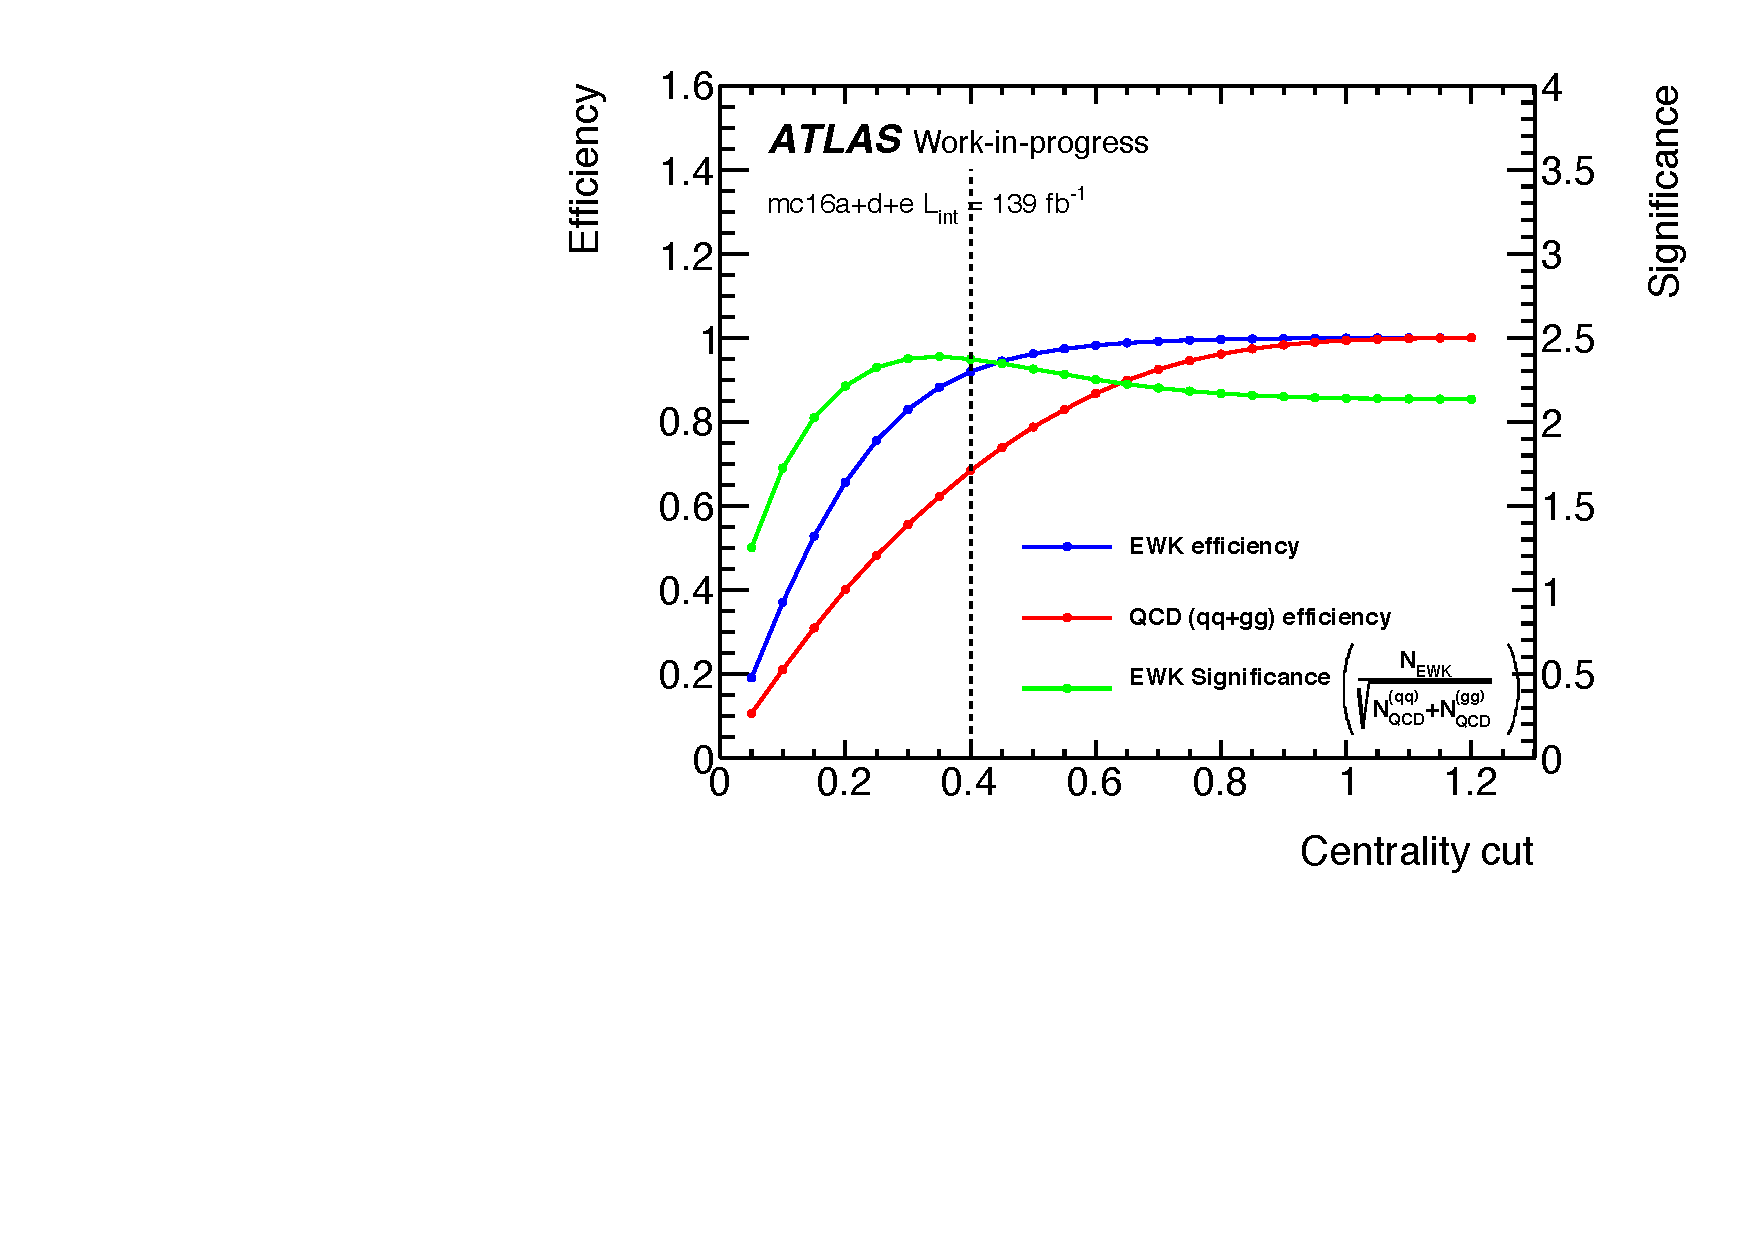
\includegraphics[width=.9\linewidth]{figures/AnalysisOverview/centrality_Cut.pdf}  \\
  \caption{Selection efficiency and EWK significance. }
  \label{fig:centrality_b}
\end{subfigure}
\caption{Centrality dependence for yield, EWK selection efficiency and EWK significance. }
\end{figure}

	\section{Datasets and Monte Carlo Simulation}
\label{sec:DataSetAndMonteCarlo}

\subsection{LHC Dataset}
\label{subsec:Dataset}

The measurement uses the LHC collision data, named the ATLAS Run-$2$ dataset collected by the ATLAS experiment during its operation in $2015$, $2016$, $2017$, and $2018$. This dataset corresponds to proton-proton collisions at the center-of-mass energy of $\sqrt(s) = 13$ TeV and total integrated luminosity of $139 \pm 2.4$ fb$^{-1}$ measured by the LUCID-2 detector \cite{ATLASLuminosityDetector}\cite{ATLASRun2IntegratedLumi}. The uncertainty on the integrated luminosity is obtained by combining the measurements of LHC runs each year. Each data-taking run period is further divided into sub-periods of one to three weeks that vary in beam and detector conditions. The dataset used in physics analyses is required to satisfy a series of data quality checks discussed in detail in Ref \cite{ATLASRun2DataTaking}. The data passing these requirements collectively form a Good Run List (GRL) consisting of several luminosity blocks (LB). Figure \ref{fig:InstLuminosity} shows the total integrated luminosity delivered by LHC in the green distribution, recorded by the ATLAS experiment in the yellow distribution and part of the GRL in the blue distribution. The plateaus correspond to the end-of-year shutdowns of LHC, and the slopes correspond to the increasing instantaneous luminosity in different data-taking periods. 

\begin{figure}
\centering
\includegraphics[width=.8\linewidth]{figures/AnalysisOverview/IntegratedLumiRun2.pdf}  
  \caption{Total integrated luminosity collected during data taking period in Run-$2$ \cite{ATLASRun2DataTaking}. }
\label{fig:InstLuminosity}
\end{figure}

The measurement uses the following data samples from the GRL,
\begin{itemize}
\footnotesize
\item{ { GoodRunsLists/data15\_13TeV/20170619/PHYS\_StandardGRL\_All\_Good\_25ns\_276262-284484\_OflLumi-13TeV-008.root}}
\item{  {GoodRunsLists/data16\_13TeV/20180129/PHYS\_StandardGRL\_All\_Good\_25ns\_297730-311481\_OflLumi-13TeV-009.root}}
\item{{ GoodRunsLists/data17\_13TeV/20180619/physics\_25ns\_Triggerno17e33prim.lumicalc.OflLumi-13TeV-010.root}}
\item{{GoodRunsLists/data18\_13TeV/20180924/physics\_25ns\_Triggerno17e33prim.lumicalc.OflLumi-13TeV-001.root}}
\end{itemize}

\normalsize

\subsection{Monte Carlo Samples }
\label{subsec:MCSamples}

As briefly mentioned in Section \ref{sec:Pheno}, MC generates the $pp \rightarrow ZZjj\rightarrow 4\ell jj$ events incorporating the matrix element calculations for the hard-scatter $ZZjj\rightarrow 4\ell jj$ production, the parton showering, hadronization, the effect of the underlying events, and pile-up. The generated events are then simulated to interact with the ATLAS material using the Geant4 simulation toolkit following the description in Ref \cite{GEANT4}. The energy deposits of the simulated events in the detectors are then digitized and reconstructed using a detector geometry corresponding to the data-taking period. Figure \ref{fig:MCGenerationSchematic} shows a schematic overview of the MC generation.
\begin{figure}
\centering
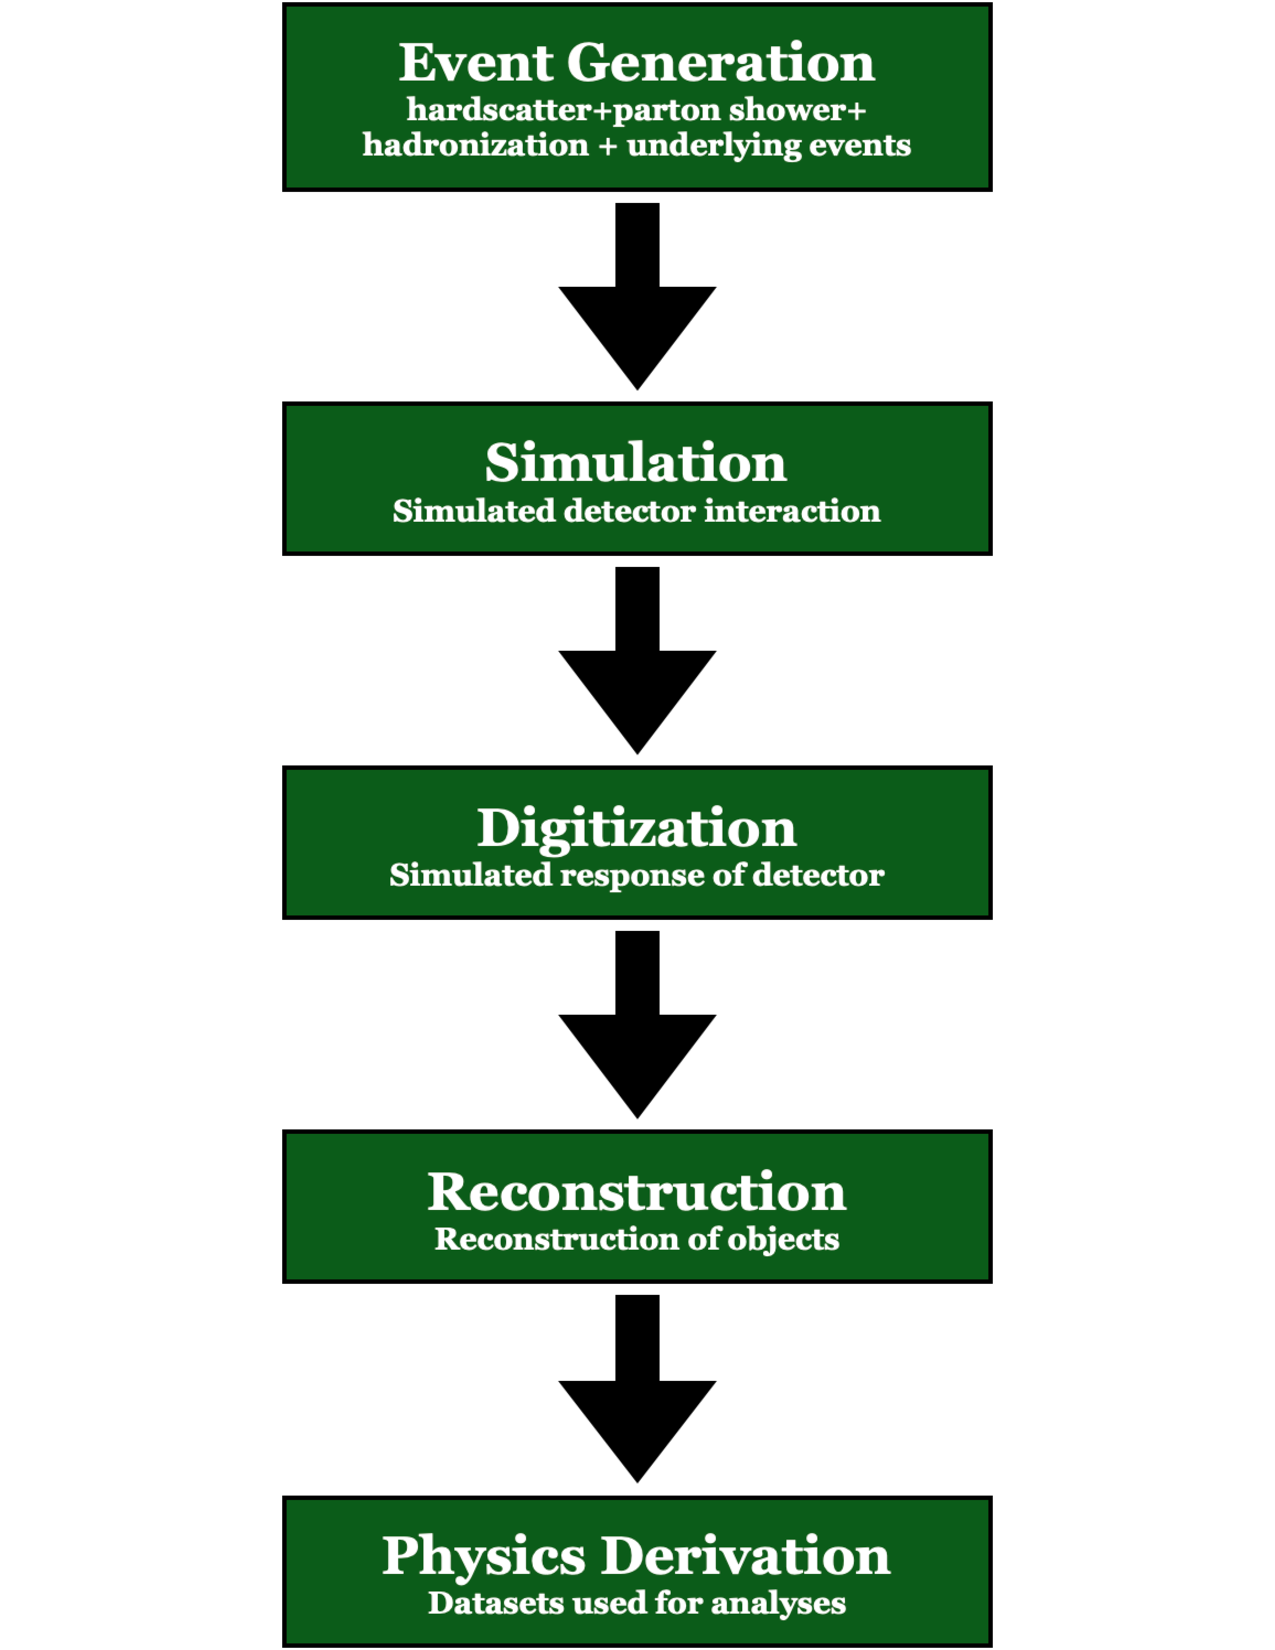
\includegraphics[width=.8\linewidth]{figures/AnalysisOverview/MCSchematic.pdf}  
  \caption{Various steps in MC sample generation.}
\label{fig:MCGenerationSchematic}
\end{figure}

\subsubsection{Signal Samples}
\label{subsubsec:SigSamples}
As discussed in section \ref{sec:EWKPheno}, two types of interaction, QCD and EWK, give us $pp \rightarrow ZZjj\rightarrow 4 \ell jj$ final state. The two types of QCD process, quark induced $qqZZ$ ($qq \rightarrow ZZ^* \rightarrow 4 \ell jj$) and gluon induced $ggZZ$ ($gg \rightarrow ZZ^* \rightarrow 4\ell jj$) are simulated using the \textsc{Sherpa} $2.2.2$ MC generator. The $qqZZ$ and $ggZZ$ samples corresponding to figure \ref{fig:ZZjjFeynmanDiag_QCD_qq} are generated with NLO accuracy in QCD up to one additional parton emission and LO accuracy for up to three additional partons emission. The loop-induced $ggZZ$ samples emerging at NNLO in $\alpha_{S}$ corresponding to figure \ref{fig:ZZjjFeynmanDiag_QCD_gg} are generated using LO-accurate matrix elements for up to one additional parton emission \cite{EventGenWithSherpa}. Results from The generator uses an NNPDF3.0NNLO PDF set evaluated using different measurements from several experiments, such as deep-inelastic inclusive cross-sections measurement from HERA-II, the combined charm data from HERA, jet production, vector boson rapidity and transverse momentum measurements from ATLAS, CMS and LHCb, total cross sections of top quark pair production from ATLAS and CMS and W+c data from CMS \cite{PDFForRunII}. Parton showering is done by \textsc{Sherpa}'s internal algorithm based on Catani–Seymour dipole factorization matrix element \cite{SherpaPS}. The matrix element calculations are matched and merged using the $ME+PS@NLO$ prescription \cite{PSMatching}. 

An alternative \textsc{MadGraph5} samples produced at NLO accuracy for up to one additional parton emission and LO accuracy for up to three additional parton emission \cite{MADGRAPHNLO} are also used in the measurement for the parton induced $qqZZ$ samples. The generator uses A14NNPDF23LO PDF set, and the ME is interfaced with \textsc{Pythia8} for parton showering, merging, and matching \cite{Pythia8}. 

The EWK production $qqZZjj$ ($qq \rightarrow ZZ^{(*)}jj \rightarrow 4 \ell jj$) is simulated using a \textsc{PowhegV2} generator using an MSTW2008 PDF set with NLO accuracy in QCD correction and interfaced with \textsc{Pythia8} for parton showering and hadronization \cite{PowhegV2}. An alternative sample at LO accuracy is also used in the measurement from \textsc{MadGraph5} with A14NNPDF23LO PDF set and \textsc{Pythia8} showering \cite{MADGRAPHNLO}. The \textsc{PowhegV2} NLO prediction of electroweak $qqZZjj$ does not contain the contribution from electroweak triboson $VZZ$ processes where two vector bosons decay leptonically and one decays hadronically. The contribution from these electroweak triboson processes is predicted using the {Sherpa} $2.2.2$ MC generator at LO accuracy for up to two additional parton emissions and added to the \textsc{PowhegV2} predictions. Table \ref{tab:SigMC} summarizes the signal MC used in the measurement. 

\begin{table}[!htb]
\footnotesize
\centering
\begin{tabular}{l l c c c }
\hline\hline
Process & Description & Generator  & PDF & Accuracy\\
\hline \hline
QCD & 		& 		 & 		 & 	 \\
\multirow{2}{*}{ $q\bar{q} \rightarrow ZZ^{(*)} \rightarrow 4\ell$ } 
					& \multirow{2}{*}{inclusive} & \textsc{Sherpa}$2.2.2$ & NNPDF3.0NNLO & \multirow{2}{*} {$0,1 j @NLO + 2,3 j @LO $} \\ 
 		&  & \textsc{MadGraph} & A14NNPDF23LO & \\
		& 		& 		 & 		 & 	 \\
\hline
QCD $gg$ loop& 		& 		 & 		 & 	 \\
 $gg \rightarrow ZZ^{(*)} \rightarrow 4\ell$ &  $m_{4 \ell } > 130$ GeV  & \textsc{Sherpa}$2.2.2$ & NNPDF3.0NNLO & $0,1 j @LO $ \\

& 		& 		 & 		 & 	 \\

\hline 
EWK & 		& 		 & 		 & 	 \\
\multirow{2}{*}{ $q\bar{q} \rightarrow ZZ^{(*)}jj \rightarrow 4\ell jj$ } 
					& \multirow{2}{*}{$m_{4\ell} > 130$ GeV } & \textsc{PowhegV2} & MSTW2008 &  $\ge 2 j$ (EWK) @ NLO QCD \\ 
 		&   & \textsc{MadGraph} & A14NNPDF23LO & $\ge 2 j$ (EWK) @LO \\
		& 		& 		 & 		 & 	 \\
\hline 
EWK  $q\bar{q} \rightarrow ZZ^{(*)}jj \rightarrow 4\ell jj$ & 		& 	\textsc{Sherpa}$2.2.2$	 & 	NNPDF3.0NNLO	 & $1,2j @LO$	 \\
\hline\hline

\end{tabular}
\normalsize
\caption{List of signal MC samples used in the analysis. Each process consists of three different generation campaigns corresponding to the data-taking conditions of the ATLAS Run2 data-taking periods.\\ \label{tab:SigMC}}
\end{table}

\subsubsection{Background Samples}
\label{subsubsec:BkgSamples}

In addition to the QCD and EWK production discussed above, two other processes, triboson ($WWZ, ~WZZ, ~ZZZ$) and $Z$-bosons production in association with top quark pair ($t\bar{t}Z$), also contributes to the $ZZjj\rightarrow 4\ell jj$ final state. The triboson processes are modeled with \textsc{Sherpa}$2.2.2$ generator at NLO accuracy in QCD for zero or one additional parton emissions and LO accuracy for up to two additional parton emissions. The triboson samples only include the fully leptonic decays of the vector bosons. Therefore, there is no overlap between the background triboson and the signal EWK $qqZZjj$ samples. The $t\bar{t}Z$ processes are modeled by \textsc{Sherpa}$2.2.0$ generator at LO accuracy with up to one additional parton emission using the MEPS@LO set-up \cite{Sherpa220}. The same algorithms as in the QCD $qqZZ$ sample generation are used for parton showering, matching, and merging. The MC simulation of the triboson and $t\bar{t}Z$ samples are subtracted directly from the data. Table \ref{tab:BkgMC} summarizes the details of these samples. 

\begin{table}[!htb]
\footnotesize
\centering
\begin{tabular}{l l c c c }
\hline\hline
Process & Description & Generator  & PDF & Accuracy\\
\hline \hline
 & 		& 		 & 		 & 	 \\
 $pp \rightarrow W^{(*)}W^{(*)}Z^{(*)} \rightarrow 4\ell 2\nu $  & \multirow{3}{*}{inclusive} & \textsc{Sherpa}$2.2.2$ & \multirow{3}{*}{NNPDF3.0NNLO} & \multirow{3}{*}{$0,1 j @NLO + 2 j @LO $} \\ 
 
$pp \rightarrow W^{(*)}Z^{(*)}Z^{(*)} \rightarrow 5\ell 1\nu$  &  & \textsc{Sherpa}$2.2.2$ &   &  \\ 
$pp \rightarrow Z^{(*)} Z^{(*)} Z^{(*)} \rightarrow 6\ell $ &  & \textsc{Sherpa}$2.2.2$ &  &  \\ 
 		
\hline 
& 		& 		 & 		 & 	 \\
$pp \rightarrow t\bar{t}+Z(\rightarrow 2\ell)$ & $m_{ll} > 5$ GeV & \textsc{Sherpa}$2.2.0$ & NNPDF3.0NNLO & LO \\

\hline\hline

\end{tabular}
\normalsize
\caption{List of background MC samples used in the analysis. Each process consists of three different generation campaigns corresponding to the data-taking conditions of the ATLAS Run2 data-taking periods.\\ \label{tab:BkgMC}}
\end{table}

\subsubsection{Samples for Fake Background}
\label{subsubsec:FakeBkgSamples}
In addition to the triboson and $t\bar{t}$Z samples, the analysis has additional backgrounds coming from events with one or more non-prompt or fake leptons. These fake backgrounds are estimated using a data-driven method discussed in detail in Section \ref{subsec:FakeBackground}. MC samples are used to develop and validate the data-driven fake background estimation procedure. There are three sources of events that could contribute as a source for fake background events. The first type of events is from a Z-boson production in association with jets $pp \rightarrow Z^{(*)} \rightarrow 2\ell +jets$, which is simulated for both three or more leptons using \textsc{Sherpa}$2.2.1$. The subdominant process is events from $t\bar{t}\rightarrow 2\ell$ production in which both top quarks decay semileptonically, which is simulated with
\textsc{Powheg+Pythia8} and uses the A14NNPDF23LO PDF set \cite{PowhegPythia}. The third type of fake backgrounds arises from the WZ production in which both bosons decay leptonically $pp \rightarrow WZ \rightarrow 2 \ell 1\nu $ and is simulated using \textsc{Sherpa}$2.2.2$. Table \ref{tab:FakeBkgMC} summarizes the different processes and MC generators used to estimate the fake background.

\begin{table}[!htb]
\footnotesize
\centering
\begin{tabular}{l l c c c }
\hline\hline
Process & Description & Generator  & PDF & Accuracy\\
\hline \hline
 & 		& 		 & 		 & 	 \\
 $pp \rightarrow Z^{(*)} \rightarrow 2e+jets $  & \multirow{3}{*}{inclusive} & \multirow{3}{*}{\textsc{Sherpa}$2.2.2$} & \multirow{3}{*}{NNPDF3.0NNLO} & \multirow{3}{*}{$NLO+2j,LO+4j $} \\ 
 
$pp \rightarrow Z^{(*)} \rightarrow 2\mu +jets $  &  &  &   &  \\ 
$pp \rightarrow Z^{(*)} \rightarrow 2\tau +jets $ &  &  &  &  \\ 
 		
\hline 
& 		& 		 & 		 & 	 \\
$pp \rightarrow t\bar{t} \rightarrow 2\ell $ & inclusive & \textsc{Powheg+Pythia8} & A14NNPDF23LO & LO \\
\hline 
& 		& 		 & 		 & 	 \\
$pp \rightarrow WZ \rightarrow 2 \ell 1\nu $ & inclusive & \textsc{Sherpa}$2.2.2$ & NNPDF3.0NNLO & $NLO + 1j, LO+3j $\\
\hline\hline

\end{tabular}
\normalsize
\caption{List of MC samples used in the estimation and validation of the data-driven fake background estimation.\\ \label{tab:FakeBkgMC}}
\end{table}

\subsection{Event Weights}
\label{subsec:EventWt}

The raw predictions from the MC generators are completely unscaled and cannot be compared to the data from the detector directly. Each event generated by the MC needs to be scaled based on the cross-section of a given process normalized to the total sum of all the weights from events generated and multiplied by the integrated luminosity of the data-taking period. As shown by figure \ref{fig:PileupDiffRuns}, the pile-up distribution is different for the different data-taking periods. The MC-generated events are modified to correctly simulate the effect of pile-up distribution imitating that of the data. Additionally, a set of measurement-related corrections are included in the event weight. These corrections, named \textit{ scaled factors (SF)}, correct the reconstruction, identification, isolation, and trigger efficiencies in the MC to match that of measured data. The total event weight for MC generated event is a product of the normalized generator weight scaled to match the pile-up profile and all scale factors.

\begin{figure}
\centering
\includegraphics[width=.8\linewidth]{figures/AnalysisOverview/mu_ProfileRun2.pdf}
\caption{Pile-up distributions in different Run-2 data-taking period.\label{fig:PileupDiffRuns} \cite{ATLASRun2DataTaking}}
\end{figure}

	\section{Definition of Measured Observables}
\label{sec:Obs}

The primary results of the thesis are differential cross-sections of the following $11$ different kinematic observables:

\begin{itemize}

\item{	$m_{4\ell}$: invariant mass of the four-leptons (or $2$ $Z$-bosons)}
\item{ 	$m_{jj}$:  invariant mass of the dijet}
\item{	$p_{T,4\ell}$: transverse momentum of the four-leptons }
\item{	$p_{T, jj}$: transverse momentum of the dijet }
\item{	$p_{T,4\ell jj}$: transverse momentum of the four-leptons and the dijet }
\item{	$s_{T,4\ell jj}$: scalar transverse momentum of the four-leptons and the dijet }
\item{ 	$\Delta \phi _{jj}^{signed}$: difference in the azimuthal angle between the two jets in the dijet, ordered according to their rapidity,i.e. 

\begin{align*}
	\Delta \phi _{jj}^{signed} = 
	\begin{cases}
	\phi(j_1)-\phi(j_2) & \text{if $y_{j_1} > y_{j_2}$}\\
	\phi(j_2)-\phi(j_1) & \text{otherwise}
	\end{cases} 
\end{align*}
}
\item{ $\Delta y_{jj}$: the absolute value of rapidity difference between the leading and the sub-leading jets in the dijet}
\item{ $\zeta$: centrality of the system}
\item{ $\cos \theta^{*}_{\ell 1 \ell 2}$: cosine of the decay angle of the negative lepton of the leading pair in the pair's rest frame as shown by figure \ref{fig:costhetaFrameOfRef}}
\item{ $\cos \theta^{*}_{\ell 3 \ell 4}$: cosine of the decay angle of the negative lepton of the sub-leading pair in the pair's rest frame as shown by figure \ref{fig:costhetaFrameOfRef} }

\end{itemize}

\begin{figure}
\centering
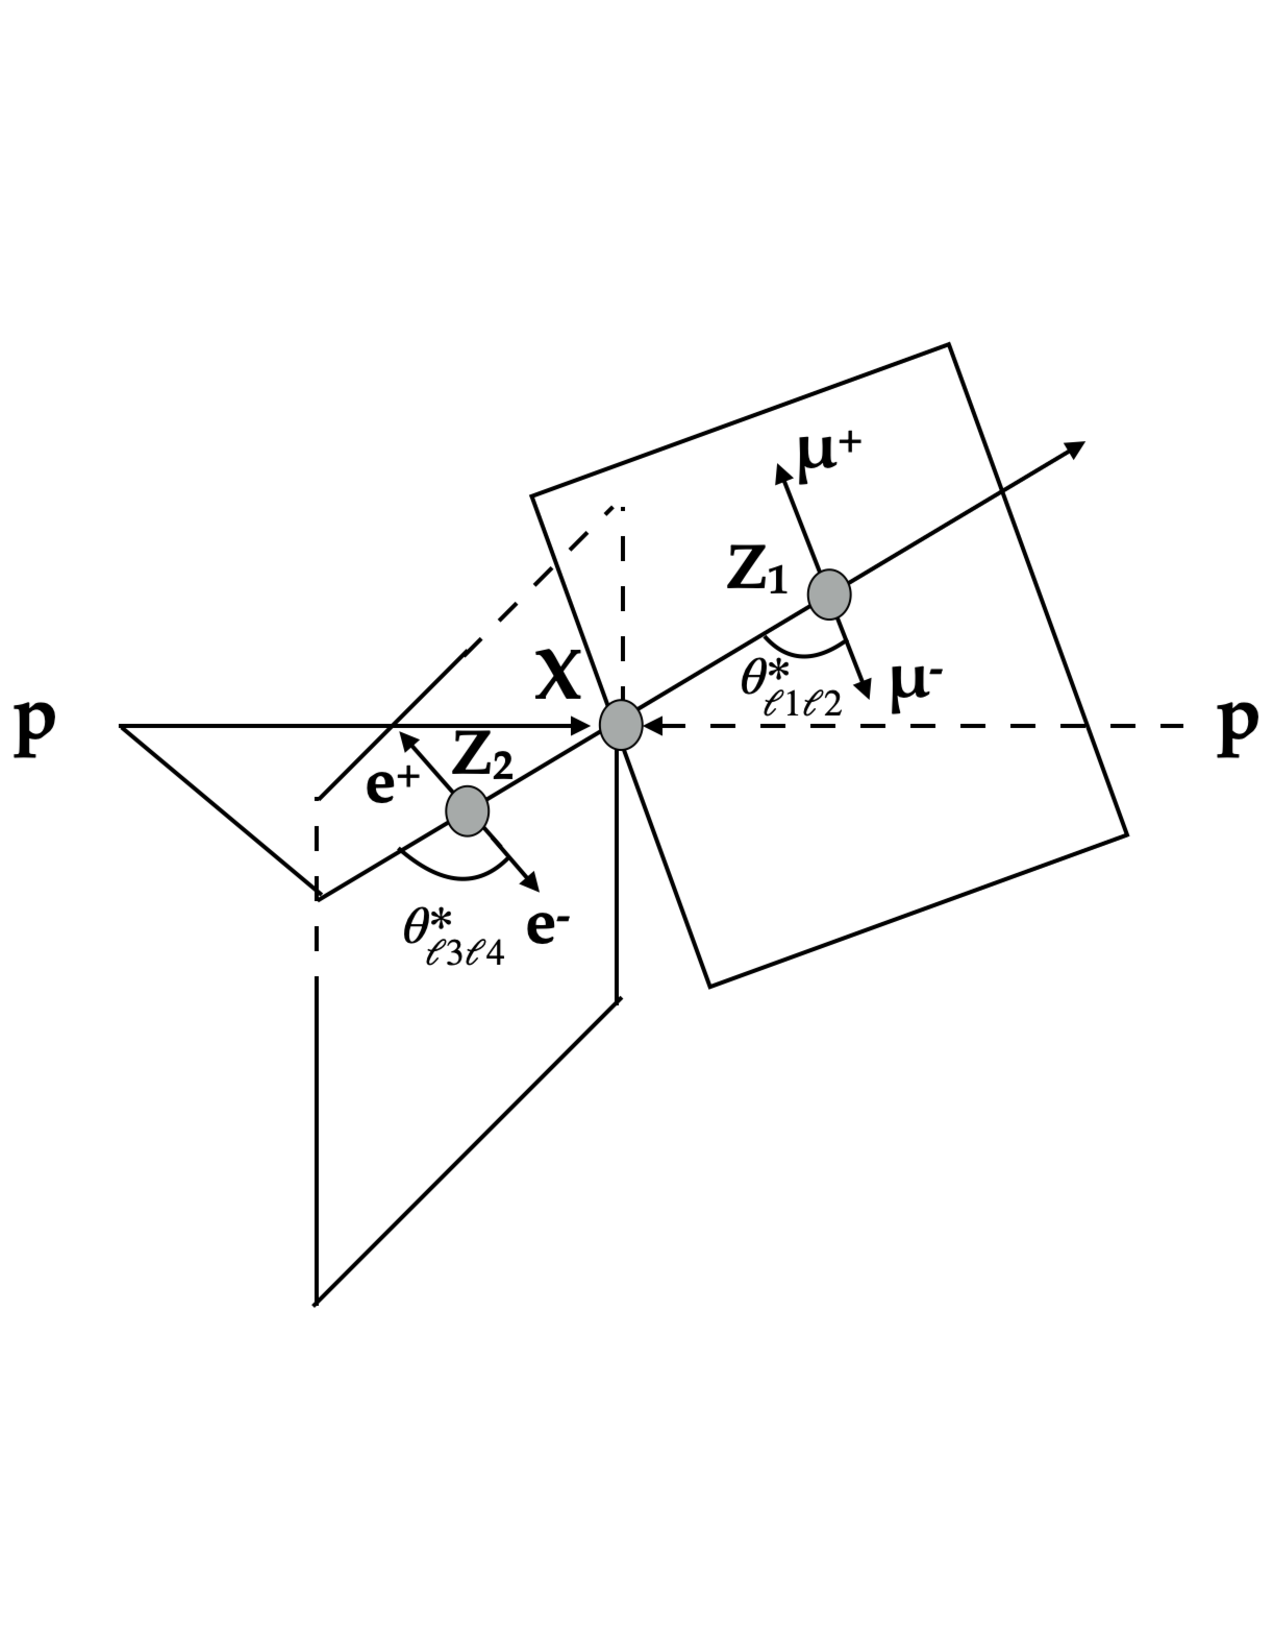
\includegraphics[width=.8\linewidth]{figures/AnalysisOverview/costhetaFrameOfRef.pdf}
\caption{Figure showing the decay angle $\theta^{*}_{\ell 1 \ell 2}$ ( $\theta^{*}_{\ell 3 \ell 4}$ ) of the negative lepton in the primary (secondary) pair's rest frame.\label{fig:costhetaFrameOfRef}\cite{AngularFrameDef}.}
\end{figure}

\clearpage

\part {\LARGE{Analysis Strategy}}
\label{sec:Analysis Strategy}

\section{Background Estimation}
\label{sec:Bkg}
In addition to the three signal physics processes, parton initiated $qqZZ$, gluon-loop initated $ggZZ$ and EWK $qqZZjj$, background processes such as $ttV$, $VVV$ and fake background comprising of \textit{non-prompt} leptons also contribute to the $ZZ(\rightarrow 4\ell) jj$ final state. As discussed in Section \ref{subsec:MCSamples} the events originating from $ttV$ and $VVV$ processes are simulated using MC generators and subtracted from data.

\subsection{Data Driven Estimate of Fake Background}
\label{subsec:FakeBackground}

\textit{Non-prompt leptons} originate from a non-hard scatter source, either from a secondary interaction such as jet decay or from charged tracks misidentification. Figure \ref{fig:NonPromptLepton} shows an example of non-prompt lepton production. The hard scatter process produces a b-jet which in secondary interaction produces a muon whose track does not point towards the interaction vertex and is surrounded by jet activities. The signal lepton criteria of isolation and TTVA discussed in Section \ref{sec:ObjReconstruction} discards most of the non-prompt leptons. However, some non-prompt leptons pass the signal criteria and, in association with other prompt leptons, form a quadruplet in the signal region. Thus, giving rise to the \textit{fake background} or \textit{non-prompt background} events for the analysis. The origins of non-prompt leptons are discussed in detail in Section \ref{subsubsec:LepComp}.

\begin{figure}
    \centering
    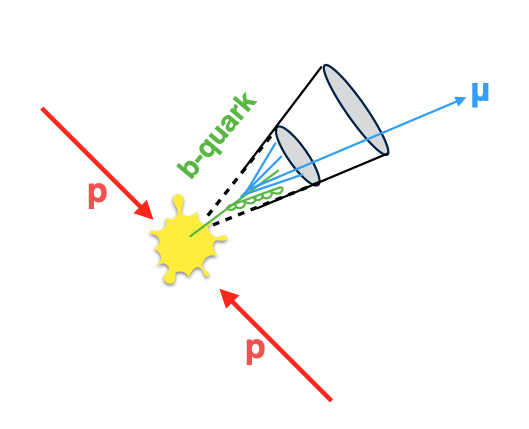
\includegraphics[width=.7\linewidth]{figures/Analysis/Background/NonPromptLeptonExample.png}  
    \caption{A schematic of the non-prompt lepton from semi-leptonic decays of b-hadrons. Jet activities surround the non-prompt muon, and the muon track does not point to the hard scatter interaction point.\label{fig:NonPromptLepton}}
\end{figure}

The fake backgrounds could be predicted using the MC for $Z(\rightarrow \ell \ell) + jets $, $t\bar{t}$ and $WZ$ processes where one or more non-prompt leptons in association with the prompt leptons form a signal quadruplet. However, it is difficult to predict the statistically limited contribution of fake background precisely using MC generators. It is also challenging to precisely model the non-prompt leptons originating from the reconstruction effects. Therefore, the fake backgrounds are estimated using an entirely data-driven technique discussed in this Section. Figure \ref{fig:FakeBkgOverview} shows the schematic of the whole background estimation process. The fake factors are evaluated from a combined control region (CR), formed by combining two independent control regions $Z+jets$ and $t\bar{t}$. Both regions are enriched in non-prompt leptons, and the combination is discussed in Section \ref{subsubsec:CR}. Section \ref{subsubsec:EstimationStrategy} discusses the technical aspects of the fake factor method, and Section \ref{subsubsec:FakeEff} discusses the fake efficiencies. The fake background is estimated by applying the fake factors to each anti-signal lepton in not-signal quadruplets. First, the background estimation technique is validated in fake-enriched validation regions discussed in Section \ref{subsubsec:Validation} and applied to the signal region, which is discussed in Section \ref{subsubsec:SREstimation}. 

\begin{figure}
    \centering
    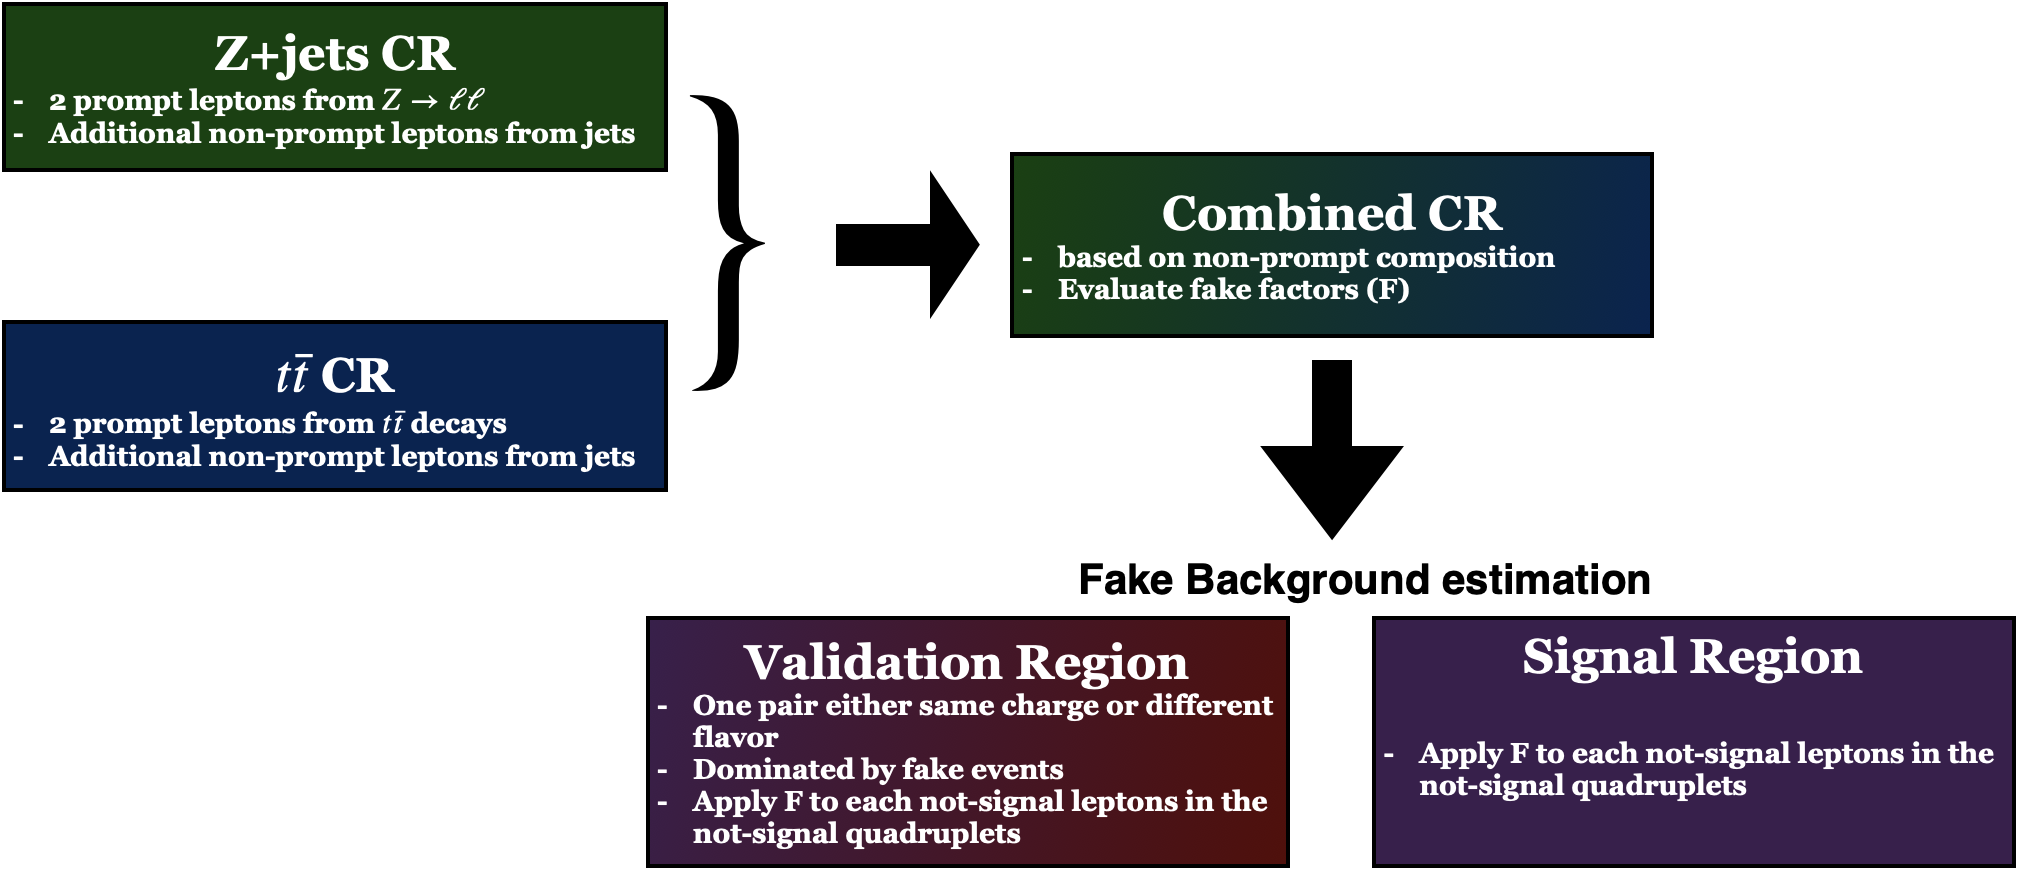
\includegraphics[width=.99\linewidth, angle =0]{figures/Analysis/Background/FakeBackgroundOverview.png}  
    \caption{An overview of the fake background estimation.\label{fig:FakeBkgOverview}}
\end{figure}

\subsubsection{Lepton Composition}
\label{subsubsec:LepComp}
The fake background MC predictions provide essential insight into the origin of the non-prompt leptons. A classification tool\footnote{https://gitlab.cern.ch/atlas/athena/-/tree/21.2/PhysicsAnalysis/AnalysisCommon/TruthClassification} developed by the ATLAS Isolation and Fake Forum (IFF) identifies the true origin of the leptons, which is studied to understand the composition of non-prompt leptons in various phase-space regions of the analysis. The tool has the following classification of truth origin for a non-prompt lepton

\begin{itemize}
    \item{ \textit{Unknown or KnownUnknown}: leptons with insufficient truth-level information to be classified by the tool.}
 
    \item { \textit{IsoElectron}: electrons originate either from the hard scatter or a boson decay. These electrons are treated as prompts in signal and background control regions.}
    
    \item{ \textit{ChargeFlipIsoElectron}: electrons whose charge is mismeasured at detector level and is classified as a non-prompt.}
    
    \item{ \textit{PromptMuon}: muons originate from either the hard scatter or a boson decay. These muons are treated as prompts for signal and background control regions.}
    
    \item{\textit{PromptPhotonConversion}: non-prompt electrons originating from photon conversion. }
    
    \item{\textit{TauDecay}: leptons originating from tau decays are treated as prompt leptons.}
    
    \item{\textit{BHadronDecay}: leptons originating from hadrons containing a b-quark. These types of leptons are one of the primary sources of non-prompt leptons.}
    
    \item{\textit{CHadronDecay}: leptons originating from hadrons containing a c-quark.}
    
    \item{\textit{LightFlavourDecay}: leptons originating from mesons and lighter hadrons.}

\end{itemize}

Figure \ref{fig:LeptonCompositionSRVBS} shows the origin of all leptons that are part of the quadruplet in the events with a signal quadruplet and a dijet. Most of the leptons in these regions are prompt and predominantly originate from $ggZZ$, $qqZZ$, and $ EWK qqZZjj$ processes. The leptons are classified \textit{Unknown/KnownUnknown} due to insufficient truth information and mainly originate from $ttZ(\rightarrow \ell \ell)$ and $VVV$ processes. Due to technical implementation in these simulation it lacks information on the intermediary bosons for these samples, thus failing to identify the lepton origin. The \textit{Unknown/KnownUnknown} leptons are treated as prompt leptons in the signal region. This treatment relies on the fact that $\Delta R$ between the \textit{Unknown/KnownUnknown} classified truth leptons and reconstruction level lepton is observed to be close to $0$. The \textit{Unknown/KnownUnknown} classified leptons are treated as non-prompt leptons in the background control regions. 

Figure \ref{fig:NonPromptLepSRDijet} shows the predicted fraction of non-prompt electrons (left) and non-prompt muons (bottom) in the events with a signal quadruplet and a dijet. The non-prompt leptons originating from $b$-hadrons or $c$-hadrons are collectively called \textit{heavy flavor (HF)} non-prompt leptons whereas, all other non-prompt leptons are categorized as \textit{light flavor (LF)}. About $50\%$ of non-prompt electrons in the signal region originate from heavy flavor sources, whereas more than $90\%$ of non-prompt muons originate from the heavy flavor decays.

\begin{figure}[htb]
    \centering
    \includegraphics[width = 0.8\textwidth]{figures/Analysis/Background/AllLeptonSRDijetComposition.pdf}
    \caption{ Origins of leptons in the signal region in events with a quadruplet and a dijet. The lepton origin is classified by the IFF classifier tool. Only leptons that are part of the signal quadruplet are shown.\label{fig:LeptonCompositionSRVBS}}
\end{figure}

\begin{figure}[htb]
    \centering
    \includegraphics[width = 0.49\textwidth]{figures/Analysis/Background/NonPromptElectronSRVBSComposition.pdf}
    \includegraphics[width = 0.49\textwidth]{figures/Analysis/Background/NonPromptMuonSRVBSComposition.pdf}
    \caption{ Origins of non-prompt electrons (left) and muons (right) in the signal region in events with a signal quadruplet and a dijet. The events are normalized to the number of non-prompt electrons (left) and non-prompt muons (right). \label{fig:NonPromptLepSRDijet}}
\end{figure}

\subsubsection{Control Regions}
\label{subsubsec:CR}
The fake factors are measured from data in a fake enriched background control region formed by combining two independent control regions, the $Z+jets$ control region and the $t\bar{t}$ control region. An event in the control regions consist of a prompt lepton pair from physics process and additional leptons from non-prompt sources. Both control regions use a single or di-lepton trigger similar to the signal region and require the leading and sub-leading leptons in an event to satisfy $p_{T,~leading~lepton} > 20$ GeV and $p_{T,~sub-leading~lepton} > 15$ GeV. An event in the $Z+jets$ CR consists of an SF-OC prompt-lepton pair from the Z boson decay with an invariant mass of $ 76~GeV~<~m_{\ell \ell}~<~106~GeV$, and additional leptons. Additionally, no events can have missing transverse energy higher than $50$ GeV to suppress the contamination from the $WZ$ process. Similarly, the $t\bar{t}$ CR consists of events with different flavor prompt-lepton pairs and additional leptons. An event in the $t\bar{t}$ CR requires at least one b-tagged jet to reduce the $WZ$ contamination. The b-tagging in the $t\bar{t}$ CR is performed by a flavor tagging tool described in Ref \cite{btagATLAS}.

Figure \ref{fig:FakeFractionBaseline} shows the fractions of the additional baseline electrons (left) and muons (right) that originate from a non-prompt source as a function of their $p_{T}$ in the $Z+jets$ CR and the $t\bar{t}$ CR. A high fraction ($\geq 80\%$) of baseline electrons originate from non-prompt sources in both $Z+jets$ CR and $t\bar{t}$ CR. More than $95\%$ of the low-$p_{T}$ baseline muons are from non-prompt sources in both control regions. These distributions show that most of the additional leptons in either control region are expected to be from non-prompt sources, thus,  motivating the control regions to evaluate the fake factors.

\begin{figure}[htb]
    \begin{subfigure}{.48\textwidth}
        \centering
        \includegraphics[width=.9\linewidth]{figures/Analysis/Background/FakeFractionBaselineElectrons.pdf}
        \caption{Fake-fraction of baseline electrons.}
    \end{subfigure}
    \begin{subfigure}{.48\textwidth}
        \centering
        \includegraphics[width=.9\linewidth]{figures/Analysis/Background/FakeFractionBaselineMuons.pdf}
        \caption{Fake-fraction of baseline muons.}
    \end{subfigure}
        \caption{Fraction of non-prompt electrons and muons in the $Z+jets$ and $t\bar{t}$ control regions. \label{fig:FakeFractionBaseline}}
\end{figure}

The control regions have a unique non-prompt lepton composition as shown by Figures \ref{fig:FakeCompositionCR2LElectron} and \ref{fig:FakeCompositionCR2LMuon}. More than $80\%$ of the non-prompt electrons in the $Z+jets$ CR originate from the light flavor decays, but about $60\%$ are from the light flavor decays in the $t\bar{t}$ CR. Similarly, about $80\%$ of the non-prompt muons in the $Z+jets$ CR originate from the heavy flavor, whereas more than $90\%$ are from the heavy-flavor decays in the $t\bar{t}$ CR. The non-prompt compositions of the signal region shown in Figure \ref{fig:NonPromptLepSRDijet} are different from either control region. The two independent control regions are combined to form a single control region with a similar non-prompt lepton composition as the signal region.

\begin{figure}[ht]
    \begin{subfigure}{.48\textwidth}
      \centering
      \includegraphics[width=.9\linewidth]{figures/Analysis/Background/NonPromptComposition_ZplusX_Electrons.pdf}  
      \caption{Non-prompt electrons in $Z+jets$ CR.}
    \end{subfigure}
    \begin{subfigure}{.48\textwidth}
      \centering
      \includegraphics[width=.9\linewidth]{figures/Analysis/Background/NonPromptComposition_ttbar_Electrons.pdf}
      \caption{Non-prompt electrons in $t\bar{t}$ CR.}
    \end{subfigure}
    \caption{Sources of non-prompt electrons in background control regions. Fake composition is unique in these control regions.\label{fig:FakeCompositionCR2LElectron}}
    \end{figure}

\begin{figure}[htb]
    \begin{subfigure}{.48\textwidth}
        \centering
        \includegraphics[width=.9\linewidth]{figures/Analysis/Background/NonPromptComposition_ZplusX_Muon.pdf}
        \caption{Non-prompt muons in $Z+jets$ CR.}
    \end{subfigure}
    \begin{subfigure}{.48\textwidth}
        \centering
        \includegraphics[width=.9\linewidth]{figures/Analysis/Background/NonPromptComposition_ttbar_Muons.pdf}
        \caption{Non-prompt muons in $t\bar{t}$ CR.}
    \end{subfigure}
        \caption{ Sources of non-prompt muons in $Z+jets$(left) and $t\bar{t}$(right) control regions.\label{fig:FakeCompositionCR2LMuon}}
\end{figure}

\begin{figure}[htb]
        \centering
        \includegraphics[width = 0.42\textwidth]{figures/Analysis/Background/NonPromptComposition_Combined_Electrons.pdf}
        \includegraphics[width = 0.42\textwidth]{figures/Analysis/Background/NonPromptComposition_Combined_Muons.pdf}
        \caption{ Origins of non-prompt electrons (left) and muons (right) in the combined control region. \label{fig:NonPromptCombined}}
\end{figure}

The $b$-jet requirement applied to suppress the prompt-lepton contamination from the WZ process in $t\bar{t}$ CR ensures the presence of at least one jet in all events. Therefore, events without jets in the combined control region only contain the $Z+jets$ $n_{jet}~=~0$ events. The two control regions are first weighted and combined for the events with the jets to match the heavy flavor composition of the $n_{jet}~>~0$ events in the signal region. The combination weights are evaluated by solving the following equation$:$

\begin{equation}
\begin{aligned}
\frac{\{w \times N_{Z+jets} \times f_{HF, Z+jets}\} + \{ (1-w) \times N_{t\bar{t}} \times f_{HF, t\bar{t}}\}}{\{w \times N_{Z+jets} + (1-w) \times N_{t\bar{t}} \}} = f_{HF, SR}  \\
\end{aligned}
\end{equation}
where $N$ is the total yield in the control region, $ f_{HF}$ is the ratio of the non-prompt leptons from heavy-flavor decays to total non-prompt leptons, and $w$ is the combination weight to be determined.

As the composition of non-prompt electrons and muons are different in different regions, the weights are evaluated separately for electrons and muons and estimated to be $w_{\mu} = 0.26$ and $w_{e} = 0.06$. Figure \ref{fig:NonPromptCombined} shows the composition of the non-prompt electrons and muons in the combined control region, which is formed by a weighted combination of the $Z+jets$ CR and the $t\bar{t}$ CR.

Figures \ref{fig:Add_e_ZplusX} and \ref{fig:Add_e_ttbar} show the distributions of additional baseline electrons as a function of their $p_{T}$ in the $Z+jets$ CR and $t\bar{t}$ CR, respectively, whereas, \ref{fig:Add_e_combined} show the same for the combined control region. For $Z+jets$ CR at low $p_{T}$, additional baseline electrons are overestimated in MC by about $20\%$, thus, showing the precision of MC to estimate the non-prompt leptons is limited. Similarly, Figures \ref{fig:Add_mu_ZplusX}, \ref{fig:Add_mu_ttbar} and \ref{fig:Add_mu_combined} show the distributions of additional baseline muons as a function of their $p_{T}$ in the three control regions. In $Z+jets$ CR, the low $p_{T}$ additional muons mainly originate from $Z\rightarrow \ell \ell$ process, whereas the high $p_{T}$ events originate more significantly from $t\bar{t}$ and WZ processes.

\begin{figure}[htb]
    \begin{subfigure}{.48\textwidth}
        \centering
        \includegraphics[width=.9\linewidth]{figures/Analysis/Background/Overlay_pt_Baseline_elecs_ZplusX.pdf}
        \caption{$Z+jets$ CR \label{fig:Add_e_ZplusX}}
    \end{subfigure}
    \begin{subfigure}{.48\textwidth}
        \centering
        \includegraphics[width=.9\linewidth]{figures/Analysis/Background/Overlay_pt_Baseline_elecs_ttbar.pdf}
        \caption{$t\bar{t}$ CR \label{fig:Add_e_ttbar}}
    \end{subfigure}\\
    \begin{subfigure}{.48\textwidth}
        \centering
        \includegraphics[width=.9\linewidth]{figures/Analysis/Background/Overlay_pt_Baseline_elecs_Combined.pdf}
        \caption{combined control region \label{fig:Add_e_combined}}
    \end{subfigure}
        \caption{ Additional baseline electrons as a function of $p_{T}$ in control regions. \label{fig:ControlRegionsAdditionalBaselineElectronpT}}
\end{figure}

\begin{figure}[htb]
    \begin{subfigure}{.48\textwidth}
        \centering
        \includegraphics[width=.9\linewidth]{figures/Analysis/Background/Overlay_pt_Baseline_muons_ZplusX.pdf}
        \caption{$Z+jets$ CR \label{fig:Add_mu_ZplusX}}
    \end{subfigure}
    \begin{subfigure}{.48\textwidth}
        \centering
        \includegraphics[width=.9\linewidth]{figures/Analysis/Background/Overlay_pt_Baseline_muons_ttbar.pdf}
        \caption{$t\bar{t}$ CR \label{fig:Add_mu_ttbar}}
    \end{subfigure} \\
    \begin{subfigure}{.48\textwidth}
        \centering
        \includegraphics[width=.9\linewidth]{figures/Analysis/Background/Overlay_pt_Baseline_muons_Combined.pdf}
        \caption{combined control region \label{fig:Add_mu_combined}}
    \end{subfigure}
        \caption{ Additional baseline muons as a function of $p_{T}$ in control regions. \label{fig:ControlRegionsAdditionalBaselineMuonpT}}
\end{figure}

\subsubsection{ Fake Factor Strategy }
\label{subsubsec:EstimationStrategy}

The centrally developed \textit{fake factor tool} by ATLAS IFF is used to estimate the fake background \cite{FakeBkgTool}. The tool takes the ratio of signal to baseline leptons, i.e., \textit{fake efficiency (f)}, calculated in the combined control region as an input where,

\begin{equation}
f = \frac{N_{non-prompt~signal~leptons}}{N_{non-prompt~baseline~leptons}}
\end{equation}

For a simple case of a signal region with one signal lepton, the observed signal lepton ($N^{T}$) and baseline-anti-signal lepton ($N^{L}$) can be estimated in terms of the number of prompt or real baseline leptons ($N^{B}_{R}$) and the number of non-prompt or fake baseline leptons ($N^{B}_{F}$) as

\begin{equation}
N^{T} = rN^{B}_{R}+fN^{B}_{F}
\label{eqn:NoOfTight}
\end{equation}
and 
\begin{equation}
N^{L} = (1-r)N^{B}_{R} + (1-f)N^{B}_{F}
\label{eqn:NoOfLoose}
\end{equation}
where, $r$ is the \textit{real efficiency} such that, 
\begin{equation} 
    r=\frac{N_{prompt~signal~leptons}}{N_{prompt~baseline~leptons}}
\end{equation}

Equations \ref{eqn:NoOfTight} and \ref{eqn:NoOfLoose} can be written as a $2 \times 2$ matrix equation as

\begin{equation}
    \begin{pmatrix} N^{T} \\ N^{L} \end{pmatrix} =  \begin{pmatrix} r & f \\ 1-r & 1-f \end{pmatrix} \begin{pmatrix} N^{B}_{R} \\ N^{B}_{F}\end{pmatrix}
    \label{eqn:RealFakeLepton}
\end{equation}

The number of non-prompt baseline contributions is estimated by ignoring the higher-order term of the fake efficiency as

\begin{equation}
    N_{F}^{B} =  \frac{1}{r-f}[r(N^{T}+N^{L})-N^{T}]
    \label{eqn:NfakeBaseline}
\end{equation}
Therefore, the predicted number of non-prompt signal lepton is 

\begin{equation}
    N_{F}^{T} =  \frac{f}{r-f}[r(N^{T}+N^{L})-N^{T}]
\label{eqn:NfakeSignal}
\end{equation}

The fake factor method assumes the $r\rightarrow 1$ limit, which simplifies equation \ref{eqn:NfakeSignal}. However, since the real efficiency of any measurement is less than one, this approximation overestimates the fake background. To account for this overestimation, the number of genuine baseline-anti-signal prompt leptons ($N^{L}_{R}$) are measured in MC and subtracted to get the final background yield as, 

\begin{equation}
    N_{F}^{T} =  \frac{f}{1-f}[N^{L}-N^{L}_{R}]
\label{eqn:NfakeSignalFinal}
\end{equation}
where, the coefficient \begin{equation} F=\frac{f}{1-f} \label{eqn:FakeFactor}
\end{equation} is the fake factor $F$. The method makes a typically safe assumption that the real anti-signal prompt leptons are modeled precisely in MC. As the fake efficiency $f$ is estimated from data in the combined control region, the fake factor background estimation method does not rely on any efficiencies or yield in the tight signal region.

This method can be extended to the four-lepton signal region where there are four baseline leptons, of which one or more could be non-prompt. Corresponding to the permutation of individual leptons to be either signal or baseline-anti-signal, there are $2^{4}=16$ \{$N^{TTTT}$, $N^{TTTL}$, $N^{TTLL}$,...$N^{LLLL}$ \} observations to consider. The analysis considers $N^{TTTT}$ the signal region; therefore, the background is estimated from the quadruplets with at least one baseline-anti-signal lepton.

\subsubsection{Fake Efficiency $\&$ Systematics}
\label{subsubsec:FakeEff}
Fake efficiency (f), defined in previous Section \ref{subsubsec:EstimationStrategy}, is evaluated from the combined control region using the total number of additional leptons from data as
\begin{equation}{\label{eq:fakeff}}
\begin{aligned}
f = \frac{ N_{Data}^{Signal}~-~N_{MC}^{Prompt~Signal}}{ N_{Data}^{Baseline}~-~N_{MC}^{Prompt~Baseline}}
\end{aligned}
\end{equation}
Since some additional leptons could originate from prompt sources, such contributions are estimated from MC and subtracted as shown in equation \ref{eq:fakeff}.

Figures \ref{fig:FakeFractionBaseline}, \ref{fig:ControlRegionsAdditionalBaselineElectronpT}, and \ref{fig:ControlRegionsAdditionalBaselineMuonpT} show that the fake-fraction and the total yield of the additional leptons are dependent on their transverse momentum $p_{T}$. Therefore, the fake efficiency evaluated using equation \ref{eq:fakeff} depends on the lepton $p_{T}$. Because of the low resolution of the detector in forward regions, a higher number of non-prompt leptons are expected in this region; thus, the fake efficiency depends on the leptons' pseudorapidity ($\eta$). Additionally, since the non-prompt leptons predominantly originate from jets, the fake efficiency also depends on the number of jets ($n_{jets}$) in an event. 

Figures \ref{fig:FakeEff_1D_Electron} and \ref{fig:FakeEff_1D_Muon} show the fake efficiencies for electrons and muons respectively as a function of $p_{T}$ (top-left), $\eta$ (top-right) and $n_{jets}$ (bottom-center). In case of the electrons, the fake efficiency decreases as a function of their $p_{T}$ up to $20$ GeV, but increases after this point. Since, the high-$p_{T}$ muons are most likely to originate from a prompt source, fake efficiency typically decreases as a function of $p_{T}$ for the muons. The dependency on $\eta$ is most likely from lower detector resolution causing a higher number of misidentifications and lower efficiency for TTVA.

As discussed in Section \ref{subsec:OR}, the lepton-favored overlap removal used in the analysis rejects jets if they overlap with leptons. Due to the $b-jet$ requirement in $t\bar{t}$ CR, the $njet=0$ events only consist of contributions from the $Z+jets$ CR, which does not have an explicit event requirement on the number of jets. The probability of non-prompt leptons passing the isolation requirement is higher in events with no jets or surrounding hadronic activity. Therefore, as observed, a higher fake efficiency is expected in events without jets.  

\begin{figure}[htb]
        \begin{center}
        \includegraphics[width = 0.49\textwidth]{figures/Analysis/Background/Fake_Eff_Elec_pt_1D.pdf}
        \includegraphics[width = 0.49\textwidth]{figures/Analysis/Background/Fake_Eff_Elec_eta_1D.pdf}\\
        \includegraphics[width = 0.49\textwidth]{figures/Analysis/Background/Fake_Eff_Elec_jet_n_1D.pdf} 
        \end{center}
    \caption{Fake efficiency of fake electrons measured in the combined control region from data as a function of its $p_{T}$, $\eta$, and $n_{jets}$.\label{fig:FakeEff_1D_Electron}}
\end{figure}

\begin{figure}[htb]
        \begin{center}
        \includegraphics[width = 0.49\textwidth]{figures/Analysis/Background/Fake_Eff_Muon_pt_1D.pdf}
        \includegraphics[width = 0.49\textwidth]{figures/Analysis/Background/Fake_Eff_Muon_eta_1D.pdf} \\
        \includegraphics[width = 0.49\textwidth]{figures/Analysis/Background/Fake_Eff_Muon_jet_n_1D.pdf} 
        \end{center}
    \caption{Fake efficiency of fake muons measured in the combined control region from data as a function of its $p_{T}$, $\eta$, and $n_{jets}$. \label{fig:FakeEff_1D_Muon}}
\end{figure}

The final fake efficiencies used in the data-driven fake background estimate is parametrized in three-dimensional distributions of $p_{T}$, $\eta$, and $n_{jets}$. Only two bins ($n_{jet}=0 ~\& ~ n_{jet} > 0$) are used for number of jets to reduce statistical fluctations. Figures \ref{fig:FakeEff_3D_Elec_njet0} and \ref{fig:FakeEff_3D_Elec_njet1} show the fake efficiency of an electron as a function of $p_{T} ~\&~ \eta$ for $n_{jet}=0 $ and $n_{jet}>0 $ bins, respectively. Similar distributions are shown in Figures \ref{fig:FakeEff_3D_Muon_njet0} and \ref{fig:FakeEff_3D_Muon_njet1} for muons.  

\begin{figure}[htb]
    \begin{center}
        \begin{subfigure}{.48\textwidth}
            \centering
            \includegraphics[width=.95\linewidth]{figures/Analysis/Background/njet0_FakeEfficiency3D_el_pt_eta.pdf}
            \caption{$n_{jet}=0$ events \label{fig:FakeEff_3D_Elec_njet0}}
        \end{subfigure}
        \begin{subfigure}{.48\textwidth}
            \centering
            \includegraphics[width=.95\linewidth]{figures/Analysis/Background/njet1_FakeEfficiency3D_el_pt_eta.pdf}
            \caption{$n_{jet}>0$ events \label{fig:FakeEff_3D_Elec_njet1}}
        \end{subfigure}
    \end{center}
    \caption{Fake efficiency of fake electrons measured in the combined control region from data as a function of its $p_{T}$, and $\eta$ in two slices of $n_{jets}$. \label{fig:ElecFakeEff}}
\end{figure}

\begin{figure}[htb]
        \begin{center}
        \begin{subfigure}{.48\textwidth}
            \centering
            \includegraphics[width=.95\linewidth]{figures/Analysis/Background/njet0_FakeEfficiency3D_mu_pt_eta.pdf}
            \caption{$n_{jet}=0$ events \label{fig:FakeEff_3D_Muon_njet0}}
        \end{subfigure}
        \begin{subfigure}{.48\textwidth}
            \centering
            \includegraphics[width=.95\linewidth]{figures/Analysis/Background/njet1_FakeEfficiency3D_mu_pt_eta.pdf}
            \caption{$n_{jet}>0$ events \label{fig:FakeEff_3D_Muon_njet1}}
        \end{subfigure}
        \end{center}
    \caption{Fake efficiency of fake muons measured in the combined control region from data as a function of its $p_{T}$, and $\eta$ in two slices of $n_{jets}$. \label{fig:MuonFakeEff}}
\end{figure}

The fake efficiency distributions' binomial errors are propagated as the statistical uncertainties on the fake estimate. The subtracted prompt component of equation \ref{eq:fakeff} is estimated using MC predictions. As discussed in Section \ref{sec:Pheno}, the prediction relies on the PDF, the energy-dependent QCD factorization and renormalization scale, and the strong coupling constant $(\alpha_{S})$. Therefore, the theory uncertainties on these three parameters are propagated as systematic uncertainties of the fake efficiency. 

For each theory uncertainty, a variation-applied fake efficiency is evaluated by separately varying the numerator and denominator of the fake efficiency equation \ref{eq:fakeff}. The difference between the variation-applied fake efficiency and the nominal fake efficiency is considered systematic uncertainty. Figures \ref{fig:FakeEffUnc_3D_Electron} and \ref{fig:FakeEffUnc_3D_Muon} show the statistical and systematic uncertainties on the fake efficiencies for electrons and muons, respectively as a function of their $p_{T},~\eta,~\&~n_{jets}$ calculated in the combined control region. For both electrons and muons, the statistical uncertainty is dominant.

\begin{figure}[htb]
    \begin{center}
    \begin{subfigure}{.48\textwidth}
        \centering
        \includegraphics[width=.95\linewidth]{figures/Analysis/Background/SystematicUncertainties3D_Electron_pT.pdf}
        \caption{$p_{T}$ \label{fig:FakeUnc_pt_e}}
    \end{subfigure}
    \begin{subfigure}{.48\textwidth}
        \centering
        \includegraphics[width=.95\linewidth]{figures/Analysis/Background/SystematicUncertainties3D_Electron_eta.pdf}
        \caption{$\eta$ \label{fig:FakeUnc_eta_e}}
    \end{subfigure}\\
    \begin{subfigure}{.48\textwidth}
        \centering
        \includegraphics[width=.95\linewidth]{figures/Analysis/Background/SystematicUncertainties3D_Electron_njet.pdf}
        \caption{$n_{jet}$ \label{fig:FakeUnc_njet_e}}
    \end{subfigure}
    \end{center}
\caption{Uncertainties on the fake efficiency of the fake electrons measured in the combined control region from data as a function of their $p_{T}$, $\eta$, and $n_{jets}$. \label{fig:FakeEffUnc_3D_Electron}}
\end{figure}

\begin{figure}[htb]
    \begin{center}
    \begin{subfigure}{.48\textwidth}
        \centering
        \includegraphics[width=.95\linewidth]{figures/Analysis/Background/SystematicUncertainties3D_Muon_pT.pdf}
        \caption{$p_{T}$ \label{fig:FakeUnc_pt_mu}}
    \end{subfigure}
    \begin{subfigure}{.48\textwidth}
        \centering
        \includegraphics[width=.95\linewidth]{figures/Analysis/Background/SystematicUncertainties3D_Muon_eta.pdf}
        \caption{$\eta$ \label{fig:FakeUnc_eta_mu}}
    \end{subfigure}\\
    \begin{subfigure}{.48\textwidth}
        \centering
        \includegraphics[width=.95\linewidth]{figures/Analysis/Background/SystematicUncertainties3D_Muon_njet.pdf}
        \caption{$n_{jet}$ \label{fig:FakeUnc_njet_mu}}
    \end{subfigure}
    \end{center}
\caption{Uncertainties on the fake efficiency of the fake muons measured in the combined control region from data as a function of their $p_{T}$, $\eta$, and $n_{jets}$. \label{fig:FakeEffUnc_3D_Muon}}
\end{figure}

\subsubsection{Method Validation}
\label{subsubsec:Validation}
Before implementing the fake-factor method to estimate the fake background in the signal region, the method is validated in two separate validation regions
\begin{enumerate}
    \item{ Different-flavor validation region (VRDF): one pair in the quadruplet must have two different-flavor leptons.}
    \item{ Same-charge validation region (VRSC): one pair in the quadruplet must have two same-charge leptons.}
\end{enumerate}

The low statistics in both regions result from requiring one of the pairs in the quadruplet to be either same-charge or different-flavor. Therefore, only signal quadruplets are required in the validation regions events without any dijet requirement. The validation regions' quadruplets are formed by requiring the same kinematic criteria as that of the signal region discussed in Section \ref{sec:EventSel}. The trigger requirement, object selection, and overlap removal are identical to the signal region. Additionally, events in the VRDF are required not to have any b-tagged jet to reduce the contribution from $ttZ$ processes. Reducing the $ttZ$ component further reduces the significant modeling uncertainties related to the $ttZ$ process.

By imposing either a same-charge or a different-flavor pair, the event yield in validation regions is dominated by events where at least one lepton in the quadruplet is a non-prompt-signal lepton known as the fake background in the signal region. The events also originate from other physics processes, such as $qqZZ$, $qqZZjj$, $ggZZ$, $ttZ$, and $VVV$ whose contribution is predicted by the same MC generators as that of the signal region.

Figures \ref{fig:VRDF_Elec_NonPromptComp} and \ref{fig:VRDF_Muon_NonPromptComp} show the non-prompt composition in the different flavor validation region for non-prompt electrons and muons, respectively. Similarly, Figures \ref{fig:VRSC_Elec_NonPromptComp} and \ref{fig:VRSC_Muon_NonPromptComp} show the fake composition of the non-prompt electrons and muons, respectively in same-charge validation region. The non-prompt compositions in the two validation regions are different from that of the signal region shown in Figure \ref{fig:NonPromptLepSRDijet} or that of the background control regions composition shown in Figures \ref{fig:FakeCompositionCR2LElectron} and \ref{fig:FakeCompositionCR2LMuon}. Therefore, to validate the fake background estimation strategy, it is imperative to observe a good correspondence between data and a combination of the total MC prediction with the fake background yield in both validation regions.

\begin{figure}[htb]
    \centering
    \begin{subfigure}{.48\textwidth}
        \centering
        \includegraphics[width=.9\linewidth]{figures/Analysis/Background/NonPromptCRDFSignal_Electronss_bVeto.pdf}
        \caption{Non-prompt electrons in VRDF.\label{fig:VRDF_Elec_NonPromptComp}}
    \end{subfigure}
    \begin{subfigure}{.48\textwidth}
        \centering
        \includegraphics[width=.9\linewidth]{figures/Analysis/Background/NonPromptCRDFSignal_Muons_bVeto.pdf}\\
        \caption{Non-prompt muons in VRDF.\label{fig:VRDF_Muon_NonPromptComp}}
    \end{subfigure}
    \begin{subfigure}{.48\textwidth}
        \centering
        \includegraphics[width=.9\linewidth]{figures/Analysis/Background/NonPromptCRSCSignal_Electrons_.pdf}
    \caption{Non-prompt electrons in VRSC.\label{fig:VRSC_Elec_NonPromptComp}}
    \end{subfigure}
    \begin{subfigure}{.48\textwidth}
        \centering
        {\includegraphics[width=.9\linewidth]{figures/Analysis/Background/NonPromptCRSCSignal_Muons_.pdf}}\\
        \caption{Non-prompt muons in VRSC.\label{fig:VRSC_Muon_NonPromptComp}}
    \end{subfigure}
    \caption{ Sources of non-prompt electrons and muons in the different flavors and the same charge validation regions. \label{fig:VRNonPromptComposition}}
\end{figure}

The fake backgrounds for the validation regions are estimated by applying the fake factor to each baseline-anti-signal leptons in the not-signal quadruplet, as discussed in Section \ref{subsubsec:EstimationStrategy}. Figure \ref{subfig:VRDFMCRed} shows the data and the predicted MC yield in VRDF as a function of $m_{4\ell}$ where the fake backgrounds are estimated from $Z+jets$, $t\bar{t}$, and $WZ$ MC predictions. Figure \ref{subfig:VRDFFF} shows the same but the non-prompt background events are estimated using the fake factor method. Similarly, figures \ref{subfig:VRSCMCRed} and \ref{subfig:VRSCFF} show the yields as a function of $m_{4\ell}$ in the same charge validation region. Both regions have similar characteristics, and the fake background dominates the event yield with some contribution from other physics processes.

The systematic gray bands in figures \ref{subfig:VRDFFF} and \ref{subfig:VRSCFF} include the total systematic and statistical uncertainties from the fake factor method, as well as the uncertainties on PDF, QCD scale, and strong coupling ($\alpha_{S}$) on the $qqZZ,~qqZZjj~\&~ggZZ$ MC prediction. The bands also include the uncertainties in the cross-section measurements of the $ttZ$ and $VVV$ processes. The treatment of the systematic theoretical uncertainties is the same as that of the signal region, which will be discussed in Section \ref{subsec:TheoryUnc}. Other experimental uncertainties related to the lepton reconstruction and identification, trigger, and luminosity discussed in Section \ref{subsec:ExpUnc} are assumed to be negligible for the validation regions. For most bins, in both regions, the data and MC yield are compatible within $1\sigma$ band of the total uncertainties. Additionally, the agreement between data and MC simulation is better when the reducible events are estimated using the fake factor method, thus, fully validating the method. Moreover, it can be concluded that estimate from the fake factor method is robust in estimation regions where the lepton composition is different than that of the phase space where the fake factors were derived.

\begin{figure}[htb]
    \centering
    \begin{subfigure}{.48\textwidth}
        \centering
        \includegraphics[width = 0.9\linewidth]{figures/Analysis/Background/Overlay_VRDF_MC_M4l.pdf}
        \caption{VRDF: MC predicted fake background.\label{subfig:VRDFMCRed}}
    \end{subfigure}
    \begin{subfigure}{.48\textwidth}
        \centering
        \includegraphics[width = 0.9\linewidth]{figures/Analysis/Background/Overlay_VRDF_FFApplied_M4l.pdf}\\
        \caption{ VRDF: FF estimate of fake background. \label{subfig:VRDFFF} }
    \end{subfigure}
    \begin{subfigure}{.48\textwidth}
        \centering
        \includegraphics[width = 0.9\linewidth]{figures/Analysis/Background/Overlay_VRSC_MC_M4l.pdf}
        \caption{VRSC: MC predicted fake background.\label{subfig:VRSCMCRed}}
    \end{subfigure}
    \begin{subfigure}{.48\textwidth}
        \centering
        \includegraphics[width = 0.9\linewidth]{figures/Analysis/Background/Overlay_VRSC_FFApplied_M4l.pdf}
        \caption{VRSC: FF estimate of fake background.\label{subfig:VRSCFF}}
    \end{subfigure}
    
    \caption{ Comparison of data to the total MC prediction and fake backrgound in the different flavor (top) and same charge (bottom) validation regions as a function of $\mFourL$.\label{fig:VRDataMCYield}}
\end{figure}

The data and MC yield comparisons for several kinematic observables in VRDF (left) and VRSC (right) are shown by distributions in Figure \ref{fig:AllDataMCYield}. The data and MC prediction are compatible in most bins within the systematic uncertainties for all the observables.

\begin{figure}[htb]
    \centering
    \begin{subfigure}{.48\textwidth}
        \centering
        \includegraphics[width = 0.85\linewidth]{figures/Analysis/Background/Overlay_VRDF_FFApplied_pt1.pdf}
        \caption{VRDF: $p_{T,~leading~lepton}$}
    \end{subfigure}
    \begin{subfigure}{.48\textwidth}
        \centering
        \includegraphics[width = 0.85\linewidth]{figures/Analysis/Background/Overlay_VRSC_FFApplied_pt1.pdf}
        \caption{VRSC: $p_{T,~leading~lepton}$}
    \end{subfigure} \\
    \begin{subfigure}{.48\textwidth}
        \centering
        \includegraphics[width = 0.85\linewidth]{figures/Analysis/Background/Overlay_VRDF_FFApplied_eta1.pdf}
        \caption{VRDF: $\eta_{T,~leading~lepton}$}
    \end{subfigure}
    \begin{subfigure}{.48\textwidth}
        \centering
        \includegraphics[width = 0.85\linewidth]{figures/Analysis/Background/Overlay_VRSC_FFApplied_eta1.pdf}
        \caption{VRSC: $\eta_{T,~leading~lepton}$}
    \end{subfigure}\\
    \begin{subfigure}{.48\textwidth}
        \centering
        \includegraphics[width = 0.85\linewidth]{figures/Analysis/Background/Overlay_VRDF_FFApplied_n_jets.pdf}
        \caption{VRDF: $n_{jets}$}
    \end{subfigure}
    \begin{subfigure}{.48\textwidth}
        \centering
        \includegraphics[width = 0.85\linewidth]{figures/Analysis/Background/Overlay_VRSC_FFApplied_n_jets.pdf}
        \caption{VRSC: $n_{jets}$}
    \end{subfigure}
        \caption{ Comparison of data to the total MC prediction and fake backrgound in validation regions (left) as a function of three kinematic observables that were used to parametrize the fake efficiencies in the control regions.\label{fig:AllDataMCYield}}
\end{figure}

\subsubsection{Signal Region Estimation}
\label{subsubsec:SREstimation}
Similar to the validation regions, the background in the signal region is estimated by applying the fake factor to the not-signal quadruplets, as discussed in Section \ref{subsubsec:EstimationStrategy}. Distributions in Figure \ref{fig:MCFFRedComparison} compare the fake background predicted from MC and estimated from the fake-factor method in the VBS-Enhanced signal events as a function of $\mFourL$ (left) and $\ptFourL$ (right). Figure \ref{fig:MCFFRedStack} shows identical distributions but also includes the total SM prediction in the same region. The lower panel of the plot shows the fake background to the predicted signal ratio, which is small. The gray bands in the plots are from systematic uncertainties of the fake factor method, whose effect is negligible on the overall yield of the signal region.

\begin{figure}[htb]
    \centering
    \includegraphics[width=0.48\textwidth]{figures/Analysis/Background/MCRedCompare_VBS_Enhanced_M4l.pdf}
    \includegraphics[width=0.48\textwidth]{figures/Analysis/Background/MCRedCompare_VBS_Enhanced_Pt4l.pdf}
    \caption{ MC prediction and fake-factor method estimate of the fake background as a function of $\mFourL$(left) and $\ptFourL$ (right) in the VBS-Enhanced region. Black bands represent the systematic uncertainties from the fake factor method. \textcolor{red}{remake plots with ATLAS Label and cleaning other labels} \label{fig:MCFFRedComparison}}
\end{figure}

\begin{figure}[htb]
    \centering
    \includegraphics[width=0.48\textwidth]{figures/Analysis/Background/RedStack_VBSEnhanced_M4l.pdf}
    \includegraphics[width=0.48\textwidth]{figures/Analysis/Background/RedStack_VBSEnhanced_Pt4l.pdf}
    \caption{ SM prediction and fake background estimated from the fake-factor method as a function of $\mFourL$(left) and $\ptFourL$ (right) in the VBS-Enhanced region. Black bands represent the systematic uncertainties from the fake factor method, which are negligible on the full signal region distribution. \textcolor{red}{remake plots with ATLAS Label, cleaning other label and y-xis/ratio-axis title} \label{fig:MCFFRedStack} }
\end{figure}

\section{Unfolding}
\label{sec:Unfolding}
The main results of the thesis are differential cross-section measurements at the particle level. The inclusive detector level cross-section for a given physics process $p_{1}p_{2}\rightarrow X$ is, 

\begin{equation}
    \sigma ^{detector~level}_{p_{1}p_{2}\rightarrow X} = A \times \epsilon \times \sigma ^{particle-level}_{p_{1}p_{2}\rightarrow X}
    \label{eqn:InclusiveXS}
\end{equation}
where $\sigma ^{particle-level}_{p_{1}p_{2}\rightarrow X}$ is the \textit{true} cross-section of the physics process predicted by the theory. The physical layout of the ATLAS detector does not cover all areas of the phase space. $A$ accounts for the limited acceptance of the ATLAS detector. Several parts of the detector have several reconstruction efficiencies, which are accounted for by the factor $\epsilon$. The detector level cross-section is measured experimentally in terms of the number of particles in a given final state (N) and integrated Luminosity $L$ as $\sigma ^{detector~level}_{p_{1}p_{2}\rightarrow X} = \frac{N}{L}$. The \textit{true} particle level inclusive cross-section can be estimated by correcting for detector acceptance and detector efficiency for the measured cross-section $\sigma ^{detector~level}_{p_{1}p_{2}\rightarrow X}$.

For differential cross-sections where the cross-section is measured in different bins of the kinematic observables, additional correction is needed to correct the resolution-induced migration between nearby bins. 

This Chapter discusses the unfolding technique in detail. Section \ref{subsec:UnfoldingOverview} gives an Overview on the unfolding algorithm, whereas Section \ref{subsec:UnfoldingValidation} validates the unfolding method. Section \ref{subsec:Bias} discusses the bias from unfolding and the attempts to optimize the bias.  

\subsection{Method Overview}
\label{subsec:UnfoldingOverview}
The analysis uses an \textit{iterative Bayesian unfolding} algorithm based on Baye's theorem \cite{BayesianUnfolding} \cite{Improved_BayesianUnfolding} using ATLAS-supported \textit{RooUnfold} package \cite{RooUnfold}. Bayes' theorem formulates a mathematical relation to obtain a probability of an effect $E$ caused by several independent causes $C_{i}$, given the initial probability of the causes $P(C_{i})$ and the conditional probability of the $i-th$ cause to produce the effect $P(E|C_{i})$ as, 

\begin{equation}
P(C_{i}|E) = \frac{ P(E|C_{i}) . P(C_{i}) } { \sum_{j}{ P(E|C_{j}).P(C_{j}) } }
\label{eqn:BayesTheorem}
\end{equation}

The obtained probability depends on the prior probability of the cause and the conditional probability of cause and effect. The prior dependency is reduced by using an iterative technique, where the outcome of the previous iteration is used as a prior for the subsequent iteration.

For a single iteration, the algorithm can be summarized as, 

\begin{equation}
    U_{i} = \frac{1}{ \epsilon_{i} } \times \sum^{reco~bins}_{j}{ (R_j -F_j ) . f_{i} . \frac{M_{ji} T_{i}}{ \sum_{k}^{truth~bins}{M_{jk} T_{k}}} } 
    \label{eqn:BayesianUnfolding}
\end{equation}
where $U_{i}$ is the unfolded yield in the target bin $i$, $T_{i}$ is the predicted truth level yield in particle bin $i$, $R_{j}$ is the observed detector level yield in reco bin $j$ and $F_{j}$ is the subtracted detector level reducible background yield. $M_{ij}$ is the migration matrix element from particle level bin $j$ to detector level bin $i$. 

Based on the discussion, conceptually, three corrections from the SM MC prediction need to be applied to estimate the unfolded yield. The three unfolding inputs are 

\begin{itemize}
    \item{\textit{\textbf{Reconstruction efficiency ($\epsilon$):}} The reconstruction efficiency accounts for the limited acceptance and efficiency of the detector. Technically, it is defined as a fraction of events that pass both detector and fiducial level selection to the events passing only the fiducial level selection. }
    
    \item{\textit{\textbf{Fiducial fraction ($f$):}} The fiducial fraction accounts for events that are outside the fiducial region at the particle level, which due to limited detector resolution entered in the measured distribution. An example of such an event would be a signal $4\ell+jj$ event where one of the jets originates from pile-up instead of hard-scatter. Technically, it is defined as a fraction of events that pass both detector and fiducial level selection to the events passing only the detector level selection. }
    
    \item{\textit{\textbf{Migration matrix ($M_{ij}$):}} The migration matrix is a two-dimensional matrix that accounts for events migrated from particle level bin $j$ to detector level bin $i$. The migration matrix corrects the probability of bin migration. It is measured in MC by comparing particle and detector levels distributions for events that pass both fiducial and detector-level selections. Bin migrations result from resolution effects and smearing of the reconstructed distributions. The diagonal component of the migration matrix is related to the \textit{fiducial purity}, which corresponds to the fraction of detector-level events that originate from the same bin at the particle level.}
\end{itemize}

Figure \ref{fig:UnfoldingInputs} show all three unfolding inputs along with the purity as a function of $m_{jj}$. The reconstruction efficiency is less than $50\%$ caused by the poor jet reconstruction efficiency. The fiducial fraction and purity is smaller in lower bins of $m_{jj}$, which mainly corresponds to contribution from pileup jets faking the event selection. The normalized migration matrix shown in the second plot with the particle level prediction in $y-axis$ and the detector level prediction in $x-axis$ is diagonal.

\begin{figure}[htb]
    \centering
    \begin{subfigure}{.48\textwidth}
        \centering
        \includegraphics[width=.9\linewidth]{figures/Analysis/Unfolding/efficiencies_VBS_Enhanced.pdf}
        \caption{ reconstruction efficiency (red), fiducial fraction (yellow) and purity (blue). }
    \end{subfigure}
    \begin{subfigure}{.48\textwidth}
        \centering
        \includegraphics[width=.9\linewidth]{figures/Analysis/Unfolding/migration_matrix_VBS_Enhanced.pdf}
        \caption{migration matrix}
    \end{subfigure}
    \caption{ Unfolding inputs from SM MC as a function of $m_{jj}$.\textcolor{red}{remake first plot with ATLAS Label and stability} \label{fig:UnfoldingInputs}}
\end{figure}

\subsection{Binning for Unfolding}
\label{subsec:Binning}
Choosing optimal binning to perform the unfolding procedure for all kinematic observables effectively is imperative. Two factors drive the choice of binning; first, the necessity to have large enough bin statistics to maintain the Gaussian approximation while preserving the shape of the differential distributions, and second, the necessity to minimize large bin migrations and statistical uncertainties from unfolding. Therefore, each bin must have at least $15$ events in the VBS-Suppressed region and at least $20$ events in the VBS-Enhanced signal region. 

To maintain a good performance of the unfolding, each bin for the kinematic observable has at least $70\%$ purity except for $p_{T,4\ell jj}$ where at least $50\%$ purity is required. Moreover, for each observable, every bin width must be equal to or greater than the resolution of the same bin. The resolution in each particle-level bin is evaluated from MC by comparing the difference of particle and detector level yield for events that pass both fiducial- and detector-level event selection. The difference is fitted using Gaussian approximation, and twice the resulting standard deviation is taken as the resolution. Table \ref{tab:binning} shows the final bin choices for all the kinematic observables used in differential cross-section measurement.
.

\begin{table}
    \caption{Binning for all unfolded observables in VBS-Enhanced and suppressed regions. \label{tab:binning}}
    \begin{center}
    \begin{tabular}{ | c | c | c | }
    \hline
    Observable & Region & Binning \\
    \hline \hline
    \multirow{4}{*}{ $m_{jj}$ [GeV] } &  &  \\
        & VBS-Enhanced & [300, 400, 530, 720, 1080, 3280] \\
    & VBS-Suppressed & [300, 410, 600, 178] \\
    & &\\
    \hline
    \multirow{4}{*}{ $m_{4\ell}$ [GeV] } &  &  \\
        & VBS-Enhanced & [130, 210, 250, 304, 400, 1130] \\
    & VBS-Suppressed & [130, 226, 304, 752] \\
    & &\\
    \hline
    \multirow{4}{*}{ $p_{T,4\ell}$ [GeV] } &  &  \\
    & VBS-Enhanced & [0, 50, 80, 116, 174, 512] \\
    & VBS-Suppressed & [0, 76, 140, 424]\\
    & &\\
    \hline
    \multirow{4}{*}{ $p_{T,jj}$ [GeV] } &  &  \\
    & VBS-Enhanced & [0, 52, 82, 116, 172, 524] \\
    & VBS-Suppressed & [0, 80, 146, 448]\\
    & &\\
    \hline
    \multirow{4}{*}{ $p_{T,4\ell jj}$ [GeV] } &  &  \\
    & VBS-Enhanced & [0, 20, 42, 64, 298] \\
    & VBS-Suppressed & [0, 36, 70, 254]\\
    & &\\
    \hline
    \multirow{4}{*}{ $s_{T,4\ell jj}$ [GeV] } &  &  \\
    & VBS-Enhanced & [70, 240, 320, 420, 580, 1410] \\
    & VBS-Suppressed & [70, 330, 500, 1210]\\
    & &\\
    \hline
    \multirow{4}{*}{ $|\Delta y_{jj}|$ } &  &  \\
    & VBS-Enhanced & [2, 3.08, 3.74, 4.32, 5.06, 7.4] \\
    & VBS-Suppressed & [2, 2.94, 3.78, 5.4]\\
    & &\\
    \hline
    \multirow{4}{*}{ $\Delta \phi_{jj}^{signed}$ } &  &  \\
    & VBS-Enhanced & [$-\pi$, -2.1, 0, 2.1, $\pi$] \\
    & VBS-Suppressed & [$-\pi$,0,$\pi$] \\
    & & \\
    \hline
    \multirow{4}{*}{ $cos \theta_{\ell i\ell j}^{\ast}$ } &  &  \\
    & VBS-Enhanced & [-1, -0.5, 0, 0.5, 1] \\
    & VBS-Suppressed & [-1, 0, 1]\\
    & & \\
    \hline
    \multirow{4}{*}{ $\zeta$ } &  &  \\
    & VBS-Enhanced &[0, 0.06, 0.12, 0.18, 0.26, 0.4] \\
    & VBS-Suppressed & [0.4, 0.5, 0.64, 1.02]\\
    & &\\
    \hline
    \end{tabular}
    \end{center}
\end{table}

\subsection{Method Validation}
\label{subsec:UnfoldingValidation}
The unfolding method is validated using three different tests.

\subsubsection{MC Closure Test}
\label{subsubsec:MCClosure}

The first validation of the unfolding technique is with the SM MC. An SM-predicted detector level distribution for a kinematic observable is unfolded using the unfolding inputs from the same MC. Figure \ref{fig:unfolding_technical_closure} shows an example of the MC-based closure test for $m_{jj}$ in the VBS-Enhanced region. The blue detector-level MC prediction is unfolded using the inputs from the same MC, and the resulting black unfolded distribution is compared with the red particle-level prediction. Since both detector-level prediction and unfolding inputs are from the same MC, a perfect closure between the unfolded and particle-level distribution is observed.

\begin{figure}[!htb]
\centering
\includegraphics[width=.6\textwidth]{figures/Analysis/Unfolding/technical_closure_VBS_Enhanced.pdf}
\caption{MC technical closure test of the unfolding procedure for $m_{jj}$. The detector-level MC distribution (in blue) is unfolded with the nominal SM unfolding inputs and compared to the particle-level distribution (in red) from the same MC. A perfect closure between unfolded and particle level distribution is observed\label{fig:unfolding_technical_closure}}
\end{figure}

\subsubsection{Injection Test}
\label{subsubsec:InjectionTest}
The analysis uses a model-independent EFT approach discussed in Section \ref{sec:EFT} to constrain the effect of BSM physics. Therefore, it is essential to test the ability of the unfolding algorithm to uncover the accurate particle-level prediction from data containing BSM physics via injection test. In an injection test, a BSM physics contribution is added to the SM detector-level prediction, unfolded with the nominal SM unfolding inputs, and compared with the BSM-added particle-level distribution. Figure \ref{fig:Dim8cont} shows an injection test for $m_{jj}$ in the VBS-Enhanced region where a BSM contribution (green distribution) is added to the SM MC. The BSM contribution is from linear and quadratic contributions of an $FT0$ EFT operator. Figure \ref{fig:InjectTestResult} shows the result of the injection test. The BSM-added detector-level MC prediction (blue) is unfolded (black) using nominal SM MC unfolding inputs and compared against the BSM-added particle-level distribution (red). A small non-closure of about $5\%$ in the last bin of $m_{jj}$ is observed, which is well within the uncertainties of the unfolded distribution.

\textcolor{red}{Note to self: perhaps it makes sense to discuss EFT theory motivation in theory section?}

\begin{figure}[htb]
    \centering
    \begin{subfigure}{.48\textwidth}
        \centering
        \includegraphics[width=.9\linewidth]{figures/Analysis/Unfolding/injection_test_FT0_quad_mjj_detectorPred.pdf}
        \caption{ Detector level MC prediction with contribution from dimension$-8$ $FT0$ EFT operator. \label{fig:Dim8cont} }
    \end{subfigure}
    \begin{subfigure}{.48\textwidth}
        \centering
        \includegraphics[width=.9\linewidth]{figures/Analysis/Unfolding/injection_test_FT0_quad_mjj.pdf}
        \caption{Unfolded SM+EFT MC detector-level distribution with response matrix from SM MC. \label{fig:InjectTestResult}}
    \end{subfigure}
    \caption{ Injection test with  dimension$-8$ $FT0$ EFT operator. \textcolor{red}{remake plots with ATLAS Label} \label{fig:injection_test_FT0_quad}}
\end{figure}

\subsubsection{Physics Variation}
FFrom the previous ATLAS electroweak $ZZjj$ analysis, a slight enhancement on the central value of the EWk $ZZjj$ cross-section was measured \cite{ATLASZZjj}. The final unfolding validation tested the ability of the algorithm to recover the actual shape of particle-level distribution if a physics process cross-section was different from the SM prediction. First, as shown by figure \ref{fig:unfolding_xsec_var_QCD}, the cross-section for parton-initiated QCD $qqZZjj$ is varied by a factor equal to the total statistical uncertainty on data in the VBS-Suppressed region $\pm  15\%$. The varied detector-level distribution is then unfolded using the nominal SM MC unfolding inputs and compared with the varied fiducial level prediction. Figure \ref{fig:unfolding_xsec_var_EWK} shows the same test where the $EWK qqZZjj$ cross-section is varied by $\pm 11\%$ based on the enhanced cross-section observed in the previous measurement. In both cases, a non-closure of about $1\%$ is observed, well below the uncertainties from unfolding.

\begin{figure}[htb]
    \centering
    \begin{subfigure}{.48\textwidth}
        \centering
        \includegraphics[width=.9\linewidth]{figures/Analysis/Unfolding/QCD_xsec_variation.pdf}
        \caption{ QCD cross-section is varied by $\pm  15\%$ \label{fig:unfolding_xsec_var_QCD} }
    \end{subfigure}
    \begin{subfigure}{.48\textwidth}
        \centering
        \includegraphics[width=.9\linewidth]{figures/Analysis/Unfolding/EWK_xsec_variation.pdf}
        \caption{ EWK cross-section is varied by $\pm 11\%$ \label{fig:unfolding_xsec_var_EWK}}
    \end{subfigure}
    \caption{ Unfolding validation using physics variation where parton-initiated QCD (left) or the EWK process cross-sections are varied. \label{fig:unfolding_xsec_var}}
\end{figure}

\subsection{Bias and Optimization}
\label{subsec:Bias}

The unfolded procedure relies on a prior value depending on the SM MC which naturally biases the unfolded cross-sections. With each iteration of unfolding, the algorithm improves the knowledge of the prior, thus, reducing the unfolding bias. However, with increasing number of iterations, the repeated bin migrations amplifies the statistical fluctuations in data, resulting in larger values of statistical uncertainties. Therefore, a finite number of iteration is chosen and the resulting unfolding bias is taken as the systematic uncertainty for the measurement. 

The unfolding bias is evaluated by the \textit{data-driven closure test}, where a pseudo dataset is developed utilizing the ratio of observed data and SM-predicted detector-level yield. First, for each observable the data and MC ratio is smoothed using Friedman's Super Smoother technique \cite{FriedmanSmoother}, fixing the end points to the value of ratio in the first and last bins. A reweighing function for each observable is developed to reweigh the SM fiducial- and detector-level yields. The reweighed detector-level signal-yield is then unfolded with the nominal unfolding inputs from SM and compared with the reweighed fiducial-level yield to get the final unfolding bias. Figure \ref{fig:unfolding_ddclosure} shows step-by-step procedure for the data-driven closure test. As shown by the ratio panel of figure \ref{fig:ddclosure_FinalBias}, unfolding bias of order $10\%$ is observed. 

\begin{figure}[htb]
    \centering
    \begin{subfigure}{.48\textwidth}
        \centering
        \includegraphics[width=.9\linewidth]{figures/Analysis/Unfolding/DDClosure_VBS_Suppressed_Ratio.pdf}
        \caption{ Data and MC for $m_{jj}$ \label{fig:ddclosure_DataMC}}
    \end{subfigure}
    \begin{subfigure}{.48\textwidth}
        \centering
        \includegraphics[width=.9\linewidth]{figures/Analysis/Unfolding/DDClosure_VBS_Suppressed_SmoothRatio.pdf}
        \caption{Smoothed ratio of Data and MC. \label{fig:ddclosure_DataMCSmooth} }
    \end{subfigure}\\
    \begin{subfigure}{.48\textwidth}
        \centering
        \includegraphics[width=.9\linewidth]{figures/Analysis/Unfolding/DDClosure_VBS_Suppressed_Reweighted.pdf}
        \caption{ Nominal SM (red) detector level yield and reweighted-detector level yield(green). \label{fig:ddclosure_DataMCReweighted} }
    \end{subfigure}
    \begin{subfigure}{.48\textwidth}
        \centering
        \includegraphics[width=.9\linewidth]{figures/Analysis/Unfolding/DDClosure_VBS_Suppressed_Bias.pdf}
        \caption{Unfolding bias. \label{fig:ddclosure_FinalBias} }
    \end{subfigure}
    \caption{ A step-by-step overview of the data driven closure test to get the unfolding bias.  \textcolor{red}{remake plots with ATLAS Label} \label{fig:unfolding_ddclosure}}
\end{figure}

The bias observed in figure \ref{fig:ddclosure_FinalBias} is obtained by using one number of iteration for unfolding. With a goal to reduce the unfolding bias, the data-driven closure test was repeated for several number of iterations. The resulting unfolding bias and systematic uncertainties up to $4$ iterations are shown in figure \ref{fig:BiasStatUnc}. As expected the unfolding bias decreases whereas the statistical uncertainty increases with the higher number of iteration. To balance between the statistical uncertainty and bias uncertainty, one number of iteration is chosen as optimal choice for the measurement.

\begin{figure}[htb]
    \centering
    \begin{subfigure}{.49\textwidth}
        \centering
        \includegraphics[width=.9\linewidth]{figures/Analysis/Unfolding/UnfoldingBiasIteration.pdf}
       % \caption{ Unfolding bias \label{fig:UnfoldingBiasIteration} }
    \end{subfigure}
    \begin{subfigure}{.49\textwidth}
        \centering
        \includegraphics[width=.9\linewidth]{figures/Analysis/Unfolding/StatUnc_Sup.pdf}
        %\caption{ Statistical uncertainty \label{fig:UnfoldingStatUnc}}
    \end{subfigure}
    \caption{ Unfolding bias (left) and statistical uncertainty (right) with up to $4$ unfolding iterations as a function of $m_{jj}$ in VBS-Suppressed region. \label{fig:BiasStatUnc}}
\end{figure}

Unfolding bias is the largest source of the systematic uncertainty of the analysis and is studied in detail using a MC-driven toy studies to understand the source. The observed large bias is from detector-level pileup jets at lower $p_{T}$ or higher $\eta$ that are not part of the fiducial phase space. The jet-vertex-tagger and forward-jet-vertex-tagger has lower efficiency to select the hard scattering jets at lower $p_{T}$ or higher $\eta$, thus resulting in more \textit{fiducial-fake-event} contamination. The additional MC-based studies on the unfolding bias are summarized in Appendix \ref{Appendix:Unfolding_bias}. 


\section{Uncertainties on the Measurement}
\label{sec:Uncertainties}
The differential cross-section measurements discussed in this thesis are affected by three sources of systematic uncertainties, experimental sources, theoretical sources, and intrinsic systematics related to the unfolding process. The statistical uncertainty of the measurements is dominant as data statistics limit the cross-section measurements. This section discusses the source of theoretical, experimental, and unfolding uncertainties. 

\subsection{Theoretical Uncertainties}
\label{subsec:TheoryUnc}

The following sources of theoretical uncertainties are considered in the measurement.

\begin{itemize}
\item{\textbf{Uncertainties on QCD Scale:} As discussed in Section \ref{sec:Pheno}, the theoretical predictions of cross-sections depend on the factorization scale ($\mu_{F}$) and renormalization scale ($\mu_{R}$) \cite{QCDScaleAndPDFUnc}. To account for this dependence, a QCD scale uncertainty is evaluated by scaling $\mu_{F}$ and $\mu_{R}$ independently using on-the-fly variations provided by the MC generators. The variations constitute of six-point variations of $\mu_{F}$ and $\mu_{R}$ from $-50\%$ or $+100\%$ around their nominal values of 1, such that \{$\mu_R = 0.5, \mu_F = 0.5$\}, \{$\mu_R = 0.5, \mu_F = 1.0$\}, \{$\mu_R = 1.0, \mu_F = 0.5$\}, \{$\mu_R = 1.0, \mu_F = 2.0$\}, \{$\mu_R = 2.0, \mu_F = 1.0$\}, and \{$\mu_R = 2.0, \mu_F = 2.0$\}. The final uncertainty is evaluated as the absolute envelope of the six variations. The QCD scale uncertainties are evaluated for $qqZZ$, $ggZZ$, and $EWK qqZZjj$ samples. \textcolor{red}{to add intermediate systematics plot} %Figure \ref{fig:QCDScale} shows different variations and the final envelope for QCD Scale uncertainties in the VBS Enhanced region as a function of $m_{jj}$. 

% \begin{figure}
%     \centering
%     \includegraphics[width=.8\linewidth]{figures/AnalysisOverview/mu_ProfileRun2.pdf}
%     \caption{ Evaluation of the fiducial level QCD factorization and renormalization scale uncertainties band for $qqZZ$ sample. \label{fig:QCDScale}}
% \end{figure}
}
\item{\textbf{Uncertainties on PDF $\&$ $\alpha_{S}$:}
The PDF uncertainty for Sherpa and \textsc{MadGraph5} samples that use NNPDF3.0NNLO is evaluated using the prescription described in Ref \cite{PDFForRunII} using on-the-fly variation weights. The PDF variations include a set of 100 internal variations, two additional variations from the nominal PDF reweighted to the alternative MMHT2014nnlo \cite{MMHT2014PDFs} $\&$ CT14nnlo \cite{CT14nnlo} PDF sets and variations of the strong coupling constant by $\pm0.0001$ where the nominal value of $\alpha_{S}$ is $0.118$. The total uncertainty is taken as the absolute envelope of all standard deviations of $100$ internal variations, the two alternate PDF variations, added in quadrature with the envelope of the $\alpha_{S}$ variations, 
\begin{equation}
    \sigma_{PDF}^{NNPDF3.0NNLO} = \sqrt{ [ max (\sigma_{std.~dev.~int.}, |\sigma_{MMHT2014nnlo}| , |\sigma_{CT14nnlo}|~)]^2 + \sigma_{\alpha_S}^2 }
\end{equation}

The PDF uncertainty is evaluated for $qqZZ$, $ggZZ$ and \textsc{MadGraph5} $EWK qqZZjj$ samples. \textcolor{red}{to add intermediate systematics plot}  %Figure \ref{fig:PDFScale} shows different variations and the final envelope for QCD Scale uncertainties in the VBS Enhanced region as a function of $m_{jj}$. 

% \begin{figure}
%     \centering
%     \includegraphics[width=.8\linewidth]{figures/AnalysisOverview/mu_ProfileRun2.pdf}
%     \caption{ Evaluation of the fiducial level QCD factorization and renormalization scale uncertainties band for $qqZZ$ sample. \label{fig:PDFScale}}
% \end{figure}

The electroweak $EWK~qqZZjj$ samples generated by \textsc{POWHEG-V2} do not have on-the-fly variations to evaluate the PDF uncertainty. Therefore, PDF uncertainty from the \textsc{MadGraph5} sample is taken as the PDF uncertainty for \textsc{POWHEG-V2} $EWK~qqZZjj$ samples.
}
\item{\textbf{Uncertainties on $gg\rightarrow ZZ^{(\ast)}$ NLO Corrections:}
The uncertainty is related to the NLO QCD k-factor applied to the $ggZZ$ sample \cite{ggZZNLOUnc}. The NLO QCD k-factors applied are evaluated differentially as a function of the $m_{4\ell}$. 
}

\item{\textbf{$t\bar{t}V$ $\&$ $VVV$ cross-sections:}
The experimental uncertainties on recently published cross-section measurements of the $ttV$~\cite{ATLAS_ttV} and $WZZ$~\cite{ATLAS_VVV} processes by ATLAS are propagated for the analysis. On the entire $ttV$ process, a flat conservative variation of $15\%$ is applied, taken from the cross-section measurement of $ttZ$. Similarly, for $VVV$ conservative $10\%$ variation taken from the cross-section measurement of $WWZ$ is applied to the whole $VVV$ samples.
}

\end{itemize}

As shown above, the theoretical uncertainties are process specific and are evaluated separately for each MC sample. The theory uncertainties need to be propagated to the unfolded cross-section measurements. For each theory uncertainty, variation-applied particle and detector level yields are built by substituting the varied distribution for the selected process instead of the nominal one. The variation-applied detector level yield is unfolded using the unfolding inputs from nominal SM predictions. The difference between the unfolded result to the variation-applied truth MC yields gives systematic uncertainty for each variation. In general, the theoretical variations significantly affect the predicted particle-level and detector-level yields but have a negligible impact on the shape of the distributions. Since the variation is applied to both detector and particle level yields, the resulting uncertainties from theory systematics on the unfolded cross-sections are small.

\subsection{Experimental Uncertainties}
\label{subsec:ExpUnc}
The experimental uncertainties arise from the measurement of the energy and momentum scales of the reconstructed objects and the uncertainties on object reconstruction, identification, and selection efficiencies. The following category summarizes the sources of experimental uncertainties,

\textbf{Jet Related Uncertainties: }
The analysis requires two jets in the final state. Therefore, jet reconstruction and selection uncertainties are the measurement's most significant source of systematic experimental uncertainties. 

\begin{itemize}
    \item{\textbf{Jet Reconstruction Uncertainty:}
    The jet-related uncertainties associated with reconstruction and different steps of calibration discussed in Section \ref{subsec:ParticleRecon_Jets} are provided by ATLAS-supported tool $\textit{JetUncertainties}\footnote{https://twiki.cern.ch/twiki/bin/view/AtlasProtected/JetUncertainties}$. The tool provides several configurations for jet-related uncertainties adjusted to various needs of several analyses. The measurement in this thesis uses $\textit{GlobalReduction\_FullJER}$ configuration with a total of $36$ uncertainties, each with upward and downward components, corresponding to $36\times2$ variations, $20\time 2$ variations are related to JES, and $13\times2$ to JER. $6$ of the $36$ uncertainties are related to the $\eta$ inter-calibration procedure, $4$ to the pile-up energy subtraction procedure, and $8$ to the in-situ calibration of jets. An additional source of uncertainty arises from flavor composition, flavor response, a single particle response at high $p_{T}$, and possible punch-through effects.
    }
    \item{\textbf{JVT $\&$ fJVT Uncertainties:} Additional sets of jet uncertainties ($1\times 2$) arising from the efficiencies of jet vertex selections, JVT, and fJVT cut requirements are also considered in the analysis. }
\end{itemize}

An envelope of the $13$ JER uncertainty added in quadrature with other sources gives the final impact of jet-related uncertainties. 

\textbf{Lepton Related Uncertainties: } Following categories define the lepton related uncertainties in the analysis
\begin{itemize}
    \item{\textbf{Electron Efficiencies:}
    The electron efficiency uncertainty consists of uncertainties on the trigger, identification, reconstruction,
and isolation efficiencies of electrons. These uncertainties are provided by an ATLAS-supported
tool $\textit{ElectronEffciencyCorrection} \footnote{https://gitlab.cern.ch/atlas/athena/-/tree/21.2/PhysicsAnalysis/ElectronPhotonID/ElectronEfficiencyCorrection} $. There are a total of $61$ nuisance parameters related to electron efficiencies, each with upward and downward components corresponding to $61\times2$ variations. $34\times2$ out of $61$ is related to uncertainties in identification efficiency, $25\times2$ related to the reconstruction efficiencies, and a single nuisance parameter ($1\times2$) related to the isolation efficiency and trigger efficiency scale factors.    
    }
    \item{\textbf{Muon Efficiencies:} Similar to the electrons, muon efficiency uncertainty consists of variations on the trigger, identification, reconstruction, and isolation efficiencies of muons, which are provided by another ATLAS-supported tool $\textit{MuonEfficiencyCorrections} \footnote{21https://gitlab.cern.ch/atlas/athena/-/tree/21.2/PhysicsAnalysis/MuonID/MuonIDAnalysis/MuonEfficiencyCorrections} $. In total, there are $10\times2$ nuisance parameters, sets of two ($2\times2$) variations corresponding to trigger efficiency scale factors, sets of four ($4\times2$) related to the identification and reconstructed efficiency, two sets of two ($2\times 2$) each corresponding to the isolation efficiency and track-to-vertex association efficiency. 
    }
    \item{\textbf{Electron Scale $\&$ Resolution:} The electron scale and resolution uncertainty is accounted for by two sets of nuisance parameters corresponding $2\times2$ variations. 

    }
    \item{\textbf{Muon Scale $\&$ Resolution:} For muons resolution and scale uncertainties, there are $5$ sets of nuisance parameters, $2\times2$ corresponding to the muon momentum resolution as measured separately by the Inner Detector and the Muon Spectrometer. One set of nuisance parameters ($1\times 2$) corresponds to the uncertainties on the muon momentum scale, and two sets of $2\times 2$ are associated with the uncertainties in Sagitta correction.}
\end{itemize}

\textbf{Other Experimental Uncertainties: }
\begin{itemize}
    \item{\textbf{Pileup Reweighting:} As discussed in Section \ref{subsec:EventWt}, the MC predictions are reweighted to match the pile-up profile of data. A single $1\times2$ nuisance parameter accounts for upward and downward variations in the factors used for pile-up reweighting. }
    \item{\textbf{Luminosity:} As discussed in Section \ref{subsec:Dataset}, the uncertainty in the collected integrated luminosity of $139 fb^{-1}$ is $\pm1.7\%$, which is applied as a flat variation to both particle and detector level yields. } 
\end{itemize}

The experimental uncertainties affect all detector-level MC predictions and the estimate of the fake backgrounds. The experimental uncertainties need to be propagated to the unfolded cross-sections. For each systematic variation, a detector-level signal ($qqZZ+ggZZ+EWK~qqZZjj$) and background ($ttV+VVV$) distribution is built with the varied MC predictions. The variation is also applied to the fake background estimate. The variation-applied background MC and fake backgrounds are subtracted from the variation-applied total MC prediction and then unfolded using the unfolding inputs from the nominal SM prediction. The individual systematic uncertainty corresponds to the difference between the variation-applied and nominal unfolded distributions for each variation.  

\subsection{Unfolding Uncertainties}
\label{subsec:UnfoldingUnc}
The following two uncertainties are intrinsic to the unfolding porcess itself and is included in the uncertainties for the unfolded differential cross-sections.

\begin{itemize}
    \item{\textbf{Unfolding Bias:} The unfolding bias estimated using the data-driven method discusses in Section \ref{subsec:Bias} is an inherent bias of the unfolding method and the biggest source of the systematic uncertainty for the measurement.
    }

    \item{\textbf{QCD $qqZZ$ Modeling Uncertainty:} There are known differecnces between different generators that are driven by differences in parton shower, and hadronization. Therefore, a second source of unfolding systematics is required to accounts for the differences in the unfolding input modeling for the dominant $qqZZ$ process. To avoid double-counting of the unfolding method covered by the data-driven uncertainties, an alternative $qqZZ$ sample predicted by \textsc{MadGraph5} is first reweighted to match the nominal-\textsc{Sherpa} lineshape. The relative difference reweighted detector-level distribution is unfolded using the inputs from nominal-\textsc{Sherpa} and compared with the reweighted-\textsc{MadGraph5} particle level distribution. The relative difference between these two distributions is taken as modeling systematic uncertainty. Figure \ref{fig:QCDModelUnc} shows the estimation of the modeling uncertainty for $m_{jj}$ in the VBS-Enhanced region. The ratio panel of the right plot shows the QCD modeling uncertainties which range from $2-4\%$ varying in different bins.
    
    \begin{figure}
        \centering
        \includegraphics[width=.48\linewidth]{figures/Analysis/Systematics/QCDmodel_Dist.pdf}
        \includegraphics[width=.48\linewidth]{figures/Analysis/Systematics/QCDmodel_Unc.pdf}
        \caption{The left plot shows three distributions at detector-level distributions for $m_{jj}$ in VBS-Enhanced region, red corresponding to SM predictions where $qqZZ$ is taken from \textsc{Sherpa} generator, yellow shows the same but $qqZZ$ is taken from \textsc{MadGraph5} and black shows the reweighted-\textsc{MadGraph5} distribution to match the \textsc{Sherpa} lineshape. The right plot shows reweighted-\textsc{MadGraph5} detector-level (blue) distribution which is unfolded (black) using unfolding inputs from nominal-\textsc{Sherpa} and compared to the particle-level reweighted-\textsc{MadGraph5} distribution. The ratio of right plot gives the QCD modeling uncertainties. \label{fig:QCDModelUnc}}
 \end{figure}  

    }
\end{itemize}

\subsection{Background Uncertainties}
\label{subsec:BkgUnc}
There are additional sources of uncertainties from the data-driven estimate of the fake background. The statistical and systematic uncertainties on the fake efficiency discussed in Section \ref{subsubsec:FakeEff}, estimated in the combined control region, are propagated to the final unfolded cross-section yield. First, the variation-applied fake background is calculated and subtracted from the nominal detector-level prediction for each variation. The subtracted altered distribution is then unfolded with nominal unfolding inputs. The difference between the altered-unfolded distribution and the nominal-unfolded distribution gives the impact of the background uncertainties on the unfolded cross-section measurements.

\subsection{Breakdown of the Systematic Uncertainties }
\label{subsec:SysUncBreakdown}
Tables \ref{tab:systematics_mjj_VBS_Suppressed} and \ref{tab:systematics_mjj_VBS_Enhanced} show the impact of systematic uncertainties in VBS-Suppressed and VBS-Enhanced region respectively for each bin of $m_{jj}$. In both regions and most bins, the unfolding bias is the dominant source of systematic uncertainty, followed by the jet systematics. Figure \ref{fig:systematics_mjj} shows the same systematic uncertainties schematically. Figure \ref{fig:jet_systematics_mjj} shows the impact of different categories of the jet systematic uncertainties. In most bins of $m_{jj}$, the dominant jet uncertainties are from the pileup energy correction step in the jet calibration. The uncertainties from jet eta-dependent calibration and jet energy resolution are also significant. Overall, the jet reconstruction uncertainties have about $8-9\%$ effect on each bin of the unfolded cross-sections.

\begin{table}
\centering
\begin{tabular}{|l || c | c | c | }
\hline 
Bin $m_{jj}$ [GeV] & [300, 410) & [410, 600) & [600, 1780)\\
\hline 
QCD MC modelling & 1.4 & 0.3 & \textbf{6.6 }\\
Jet & \textbf{7.8} & \textbf{6.6} & \textbf{6.3 }\\
Trigger & 0.32 & 0.07 & 0.081 \\
Leptons & 1.8 & 1.2 & 1.2 \\
PRW & 0.39 & 0.062 & 0.21\\
Theory ($qqZZ$) & 2 & 2.4 & 2.1 \\
Theory (EWK $qqZZjj$) & 0.017 & 0.01 & 0.037 \\
Theory ($ggZZ$) & 0.3 & 0.51 & 0.64 \\
MC Bkg. (ttV+VVV) & 1.6 & 1.7 & 1.6 \\
Fake Bkg. (stat + syst) & 3 & 2.3 & 1.8 \\
Luminosity & 1.7 & 1.7 & 1.7 \\
Data-Driven Closure & \textbf{12} & \textbf{6.3} & \textbf{7.1}\\
\hline
Total & 15 & 10 & 12 \\
\hline
\end{tabular}
\caption{Breakdown of the relative systematic uncertainties ($\%$) for each bin of $\mjj$ in the VBS-Suppressed region. \label{tab:systematics_mjj_VBS_Suppressed}}
\end{table}

\begin{table}
\centering
\begin{tabular}{| l || c | c | c | c | c | }
\hline \hline
Bin $m_{jj}$ [GeV] & [300, 400) & [400, 530) & [530, 720) & [720, 1080) & [1080, 3280)\\
\hline
QCD MC modelling & 2.6 & 0.27 & 0.39 & 1.3 & 3.6\\
Jet & \textbf{7.4} & \textbf{7.6} & \textbf{8.9} & \textbf{8.5} & \textbf{8.9}\\
Trigger & 0.061 & 0.078 & 0.083 & 0.053 & 0.049\\
Leptons & 1.1 & 1.1 & 1.1 & 1.1 & 1.1\\
PRW & 0.38 & 0.58 & 0.79 & 0.83 & 0.59\\
Theory ($qqZZ$) & 2.7 & 2.3 & 2.6 & 1.9 & 0.85\\
Theory (EWK $qqZZjj$) & 0.074 & 0.054 & 0.065 & 0.15 & 0.89\\
Theory ($ggZZ$) & 0.48 & 0.3 & 0.34 & 0.36 & 1.1\\
MC Bkg. (ttV+VVV) & 2.7 & 2.6 & 2.4 & 1.8 & 1.2\\
Fake Bkg. (stat + syst) & 2.4 & 2.5 & 2.5 & 1.7 & 1.5\\
Luminosity & 1.7 & 1.7 & 1.7 & 1.7 & 1.7\\
\hline
Total & 9.3 & 9 & 10 & 9.4 & 10\\
\hline
\end{tabular}
\caption{Breakdown of the relative systematic uncertainties ($\%$) for each bin of $\mjj$ in the VBS-Enhanced region. \textcolor{red}{to update including data-driven closure test. } \label{tab:systematics_mjj_VBS_Enhanced}}
\end{table}

\begin{figure}[!htb]
\centering
\includegraphics[width=.49\linewidth]{figures/Analysis/Systematics/systematics_VBS_Suppressed.pdf}
\includegraphics[width=.49\linewidth]{figures/Analysis/Systematics/systematics_VBS_Enhanced.pdf}
\caption{Systematic uncertainties as a function of $\mjj$ in the VBS-Suppressed region (left) and the VBS-Enhanced region (right). \textcolor{red}{update with ATLAS labels and data-driven closure test}}  \label{fig:systematics_mjj}
\end{figure}

\begin{figure}[!htb]
\centering
\includegraphics[width=.49\linewidth]{figures/Analysis/Systematics/jet_systematics_VBS_Suppressed.pdf}
\includegraphics[width=.49\linewidth]{figures/Analysis/Systematics/jet_systematics_VBS_Enhanced.pdf}
\caption{impact of different jet systematic uncertainties on the unfolded distribution of $\mjj$ in the VBS-Suppressed region (left) and the VBS-Enhanced region (right). \textcolor{red}{update with ATLAS labels and add data-driven closure test}  \label{fig:jet_systematics_mjj}}
\end{figure}

\subsection{Statistical Uncertainties}
\label{subsubsec:StatUnc}
How does Roo Unfold propagate the statistical uncertainties at the unfolded level???? 




\clearpage

\part {\LARGE{Results}}
\label{sec:Results}

This chapter presents the main results of this thesis. Section \ref{sec:DetectorLevel_Measurement} presents the detector-level measurements of the eleven kinematic observables introduced in Section \ref{sec:Obs}, whereas Section \ref{sec:DifferentialxS} presents the unfolded differential cross-sections. Section \ref{sec:EFT} reinterprets the unfolded cross-sections shown in Section \ref{sec:DifferentialxS} to constrain parameters of physics beyond the SM affecting the quartic gauge vertices of electroweak $ZZjj$ production. 

\section{ Detector Level Measurements }
\label{sec:DetectorLevel_Measurement}

Figure \ref{fig:reco_VBS_Enhanced_a} shows the measured detector level data and predicted detector level yield for six kinematic observables; the invariant mass of the dijet $[m_{jj}]$, invariant mass of the two $Z$ bosons $[m_{4\ell}]$, transverse momentum of the two tagging jets $[p_{T,jj}]$, transverse momentum of the two $Z$ bosons $[p_{T,4\ell}]$, transverse momentum of the two $Z$ bosons and two tagging jets $[p_{T,4\ell jj}]$, and scalar transverse momentum of the two $Z$ bosons and dijet $[s_{T,4\ell jj}]$. Similarly, Figure \ref{fig:reco_VBS_Enhanced_b} shows the same for remaining kinematic observables, cosine of the decay angle of the negative lepton of the leading (sub-leading) pair in the pair's rest frame $[\cos \theta^{*}_{\ell 1 (3) \ell 2 (4)}]$, signed difference between the azimuthal angle of two jets $[\Delta \phi _{jj}^{signed}]$, rapidity difference between two jets $[\Delta y_{jj}]$, and centrality of the system $[\zeta]$.

For each of these distributions, the measured data (black dot) is compared with state-of-the-art SM predictions, where the two QCD signal $qqZZjj$ (red) $\&$ $ggZZjj$ (blue), and the two MC predicted background, $VVV$ (yellow) and $ttV$ (purple) are taken from \textsc{Sherpa} predictions. The contribution from fake backgrounds in light pink is estimated using the data-driven method. The $qqZZjj$ electroweak signal is taken from the \textsc{PowhegV2} predictions, and the electroweak production of triboson and two jets ($VZZjj$) is taken from the \textsc{Sherpa} predictions. The vertical-solid black line on the data points represents the statistical uncertainty in the data, and the dashed black box in each bin represents the impact of the total theoretical and experimental uncertainties on the predicted detector-level yields. The impact of the total systematic uncertainties and the statistical precision each ranges from $15$ to $20\%$ depending on the bins and the distributions. 

The ratio panel in these distributions shows the data yield ratio to the total predicted yield, which agrees with the SM predictions with the uncertainties. Some discrepancies are observed in some distributions; for instance, the MC yield is underpredicted in the second bin of $m_{jj}$ and in the third bin of $m_{4l}$. However, this difference is statistically insignificant. Moreover, a slight but statistically insignificant asymmetry is also observed in the measured distribution of $\Delta \phi _{jj}^{signed}$, which in SM is expected to be symmetric. 

A simple chi-squared per degree of freedom ($\chi^2/NDF$) is estimated to quantify whether the measured data agree with the SM prediction. The $\chi^2/NDF$ takes the residual difference in each bin between the unweighted data yield and the weighted MC prediction yield, along with the statistical and systematic uncertainties for both distributions. The reported values of $\chi^2/NDF$ for each distribution in figures \ref{fig:reco_VBS_Enhanced_a} and \ref{fig:reco_VBS_Enhanced_b} show statistically good agreement between the measured data and MC predictions. 

\begin{figure}[!htb]
    \centering
    \begin{subfigure}{.49\textwidth}
        \centering
        \includegraphics[width=.98\linewidth]{figures/Results/RecoDist_VBSEnhanced/reco_mjj_SR.pdf}
        \caption{ \footnotesize{$m_{jj}$}: $\chi^2/NDF = 0.43$ }
    \end{subfigure}
    \begin{subfigure}{.49\textwidth}
        \centering
        \includegraphics[width=.98\linewidth]{figures/Results/RecoDist_VBSEnhanced/reco_m4l_SR.pdf}
        \caption{ \footnotesize{$m_{4\ell}$ }: $\chi^2/NDF = 0.49$ }
    \end{subfigure}\\
    \begin{subfigure}{.49\textwidth}
        \centering
        \includegraphics[width=.98\linewidth]{figures/Results/RecoDist_VBSEnhanced/reco_ptjj_SR.pdf}
        \caption{ \footnotesize{$p_{T,jj}$}: $\chi^2/NDF = 0.30$ }
    \end{subfigure}
    \begin{subfigure}{.49\textwidth}
        \centering
        \includegraphics[width=.98\linewidth]{figures/Results/RecoDist_VBSEnhanced/reco_pt4l_SR.pdf}
        \caption{ \footnotesize{$p_{T,4\ell}$ }: $\chi^2/NDF = 0.15$ }
    \end{subfigure}\\
    \begin{subfigure}{.49\textwidth}
        \centering
        \includegraphics[width=.98\linewidth]{figures/Results/RecoDist_VBSEnhanced/reco_ptzzjj_SR.pdf}
        \caption{ \footnotesize{$p_{T,4\ell jj}$}: $\chi^2/NDF = 0.70$ }
    \end{subfigure}
    \begin{subfigure}{.49\textwidth}
        \centering
        \includegraphics[width=.98\linewidth]{figures/Results/RecoDist_VBSEnhanced/reco_stzzjj_SR.pdf}
        \caption{ \footnotesize{$s_{T, 4\ell jj}$ }: $\chi^2/NDF = 0.24$ }
    \end{subfigure}
    \caption{Detector level distributions in the VBS-Enhanced region.}  \label{fig:reco_VBS_Enhanced_a}
\end{figure}

\begin{figure}[!htb]
    \centering
    \begin{subfigure}{.49\textwidth}
        \centering
        \includegraphics[width=.98\linewidth]{figures/Results/RecoDist_VBSEnhanced/reco_cosThetaStar1_SR.pdf}
        \caption{ \footnotesize{$\cos \theta^{*}_{\ell 1 \ell 2}$}: $\chi^2/NDF = 0.51$ }
    \end{subfigure}
    \begin{subfigure}{.49\textwidth}
        \centering
        \includegraphics[width=.98\linewidth]{figures/Results/RecoDist_VBSEnhanced/reco_cosThetaStar3_SR.pdf}
        \caption{ \footnotesize{$\cos \theta^{*}_{\ell 3 \ell 4}$ }: $\chi^2/NDF = 0.61$ }
    \end{subfigure}\\
    \begin{subfigure}{.49\textwidth}
        \centering
        \includegraphics[width=.98\linewidth]{figures/Results/RecoDist_VBSEnhanced/reco_dphi_SR.pdf}
        \caption{ \footnotesize{$\Delta \phi _{jj}^{signed}$ }: $\chi^2/NDF = 1.69$ }
    \end{subfigure}
    \begin{subfigure}{.49\textwidth}
        \centering
        \includegraphics[width=.98\linewidth]{figures/Results/RecoDist_VBSEnhanced/reco_dy_SR.pdf}
        \caption{ \footnotesize{$\Delta y_{jj}$ }: $\chi^2/NDF = 0.26$ }
    \end{subfigure}\\
    \begin{subfigure}{.49\textwidth}
        \centering
        \includegraphics[width=.98\linewidth]{figures/Results/RecoDist_VBSEnhanced/reco_centrality_SR.pdf}
        \caption{ \footnotesize{$\zeta$ }: $\chi^2/NDF = 0.50$ }
    \end{subfigure}
    \caption{Detector level distributions in the VBS-Enhanced region.}  \label{fig:reco_VBS_Enhanced_b}
\end{figure}
\section{ Unfolded Differential Cross-sections }
\label{sec:DifferentialxS}

The background-subtracted data is unfolded using the iterative Bayesian Unfolding discussed in Section \ref{sec:Unfolding}. The unfolded differential cross-sections, the main results of this thesis, are obtained by multiplying the inverse of integrated luminosity to the background-subtracted unfolded yield in each bin. The unfolded differential cross-sections for eleven kinematic observables are shown in Figures \ref{fig:unfolded_xs_VBS_Enhanced_a} and \ref{fig:unfolded_xs_VBS_Enhanced_b}. 

Each distribution of unfolded differential cross-sections is compared to two different state-of-the-art particle-level SM predictions; the first prediction where the QCD $qqZZjj$ contribution is predicted by \textsc{Sherpa} generator, and the second prediction where the QCD $qqZZjj$ contribution is predicted by \textsc{Madgraph} generator. The light-red and light-blue bands are the fiducial level systematics on the \textsc{Sherpa} and \textsc{Madgraph} particle-level cross-sections, respectively. The vertical-solid line on the unfolded cross-sections is the statistical uncertainty. In contrast, the black band represents the total systematic uncertainties on unfolded cross-sections from theoretical, experimental, and unfolding sources. The unfolded cross-sections are limited by statistical precision in all distributions and all bins. For some distributions, one or two events are found in the overflow bin resulting from bin migrations. These events are added to the content of the last bin of the unfolded distribution. 

Generally, for all distributions, the data is well modeled by the MC simulations within $2\sigma$ of the uncertainty band. Two different p-values are determined by comparing unfolded cross-sections to the two predicted cross-sections to quantify the agreement between the experimentally measured unfolded data and the SM-predicted cross-sections. The p-values are calculated based on a technique discussed in Ref\cite{pValueStat} by taking the residual and uncertainties of two weighted histograms. For all kinematic observables, the reported p-values obtained by comparing to either generator are more significant than $0.05$. Therefore, in the analyzed LHC Run-2 dataset, for the $ZZ^*(\rightarrow 4 \ell) jj$ process, all differential cross-sections in the VBS-Enhanced region are concluded to agree with the SM predictions. 

\begin{figure}[!htb]
    \centering
    \begin{subfigure}{.48\textwidth}
        \centering
        \includegraphics[width=.98\linewidth]{figures/Results/CrossSection_VBSEnhanced/xs_mjj_SR.pdf}
        \caption{ \footnotesize{$m_{jj}$: p-value(Sherpa=0.95 $\&$ MG=0.91)}}
    \end{subfigure}
    \begin{subfigure}{.48\textwidth}
        \centering
        \includegraphics[width=.98\linewidth]{figures/Results/CrossSection_VBSEnhanced/xs_m4l_SR.pdf}
        \caption{ \footnotesize{$m_{4\ell}$: p-value(Sherpa=0.84 $\&$ MG=0.45)} }
    \end{subfigure}\\
    \begin{subfigure}{.48\textwidth}
        \centering
        \includegraphics[width=.98\linewidth]{figures/Results/CrossSection_VBSEnhanced/xs_ptjj_SR.pdf}
        \caption{ \footnotesize{$p_{T,jj}$: p-value(Sherpa=0.97 $\&$ MG=0.85)}}
    \end{subfigure}
    \begin{subfigure}{.48\textwidth}
        \centering
        \includegraphics[width=.98\linewidth]{figures/Results/CrossSection_VBSEnhanced/xs_pt4l_SR.pdf}
        \caption{ \footnotesize{$p_{T,4\ell}$: p-value(Sherpa=0.98 $\&$ MG=0.94)}}
    \end{subfigure}\\
    \begin{subfigure}{.48\textwidth}
        \centering
        \includegraphics[width=.98\linewidth]{figures/Results/CrossSection_VBSEnhanced/xs_ptzzjj_SR.pdf}
        \caption{ \footnotesize{$p_{T,4\ell jj}$: p-value(Sherpa=0.92 $\&$ MG=0.80)}}
    \end{subfigure}
    \begin{subfigure}{.48\textwidth}
        \centering
        \includegraphics[width=.98\linewidth]{figures/Results/CrossSection_VBSEnhanced/xs_stzzjj_SR.pdf}
        \caption{ \footnotesize{$s_{T, 4\ell jj}$: p-value(Sherpa=0.94 $\&$ MG=0.83)}}
    \end{subfigure}
    \caption{Unfolded differential cross-sections in the VBS-Enhanced region.} \label{fig:unfolded_xs_VBS_Enhanced_a}
\end{figure}

\begin{figure}[!htb]
    \centering
    \begin{subfigure}{.49\textwidth}
        \centering
        \includegraphics[width=.98\linewidth]{figures/Results/CrossSection_VBSEnhanced/xs_cosThetaStar1_SR.pdf}
        \caption{ \footnotesize{$\cos \theta^{*}_{\ell 1 \ell 2}$: p-value(Sherpa=0.80 $\&$ MG=0.55)}}
    \end{subfigure}
    \begin{subfigure}{.49\textwidth}
        \centering
        \includegraphics[width=.98\linewidth]{figures/Results/CrossSection_VBSEnhanced/xs_cosThetaStar3_SR.pdf}
        \caption{ \footnotesize{$\cos \theta^{*}_{\ell 3 \ell 4}$: p-value(Sherpa=0.71 $\&$ MG=0.30)} }
    \end{subfigure}\\
    \begin{subfigure}{.49\textwidth}
        \centering
        \includegraphics[width=.98\linewidth]{figures/Results/CrossSection_VBSEnhanced/xs_dphi_SR.pdf}
        \caption{ \footnotesize{$\Delta \phi _{jj}^{signed}$: p-value(Sherpa=0.28 $\&$ MG=0.18)} }
    \end{subfigure}
    \begin{subfigure}{.49\textwidth}
        \centering
        \includegraphics[width=.98\linewidth]{figures/Results/CrossSection_VBSEnhanced/xs_dy_SR.pdf}
        \caption{ \footnotesize{$\Delta y_{jj}$: p-value(Sherpa=0.96 $\&$ MG=0.93)} }
    \end{subfigure}\\
    \begin{subfigure}{.49\textwidth}
        \centering
        \includegraphics[width=.98\linewidth]{figures/Results/CrossSection_VBSEnhanced/xs_centrality_SR.pdf}
        \caption{ \footnotesize{$\zeta$: p-value(Sherpa=0.87 $\&$ MG=0.73)} }
    \end{subfigure}
    \caption{Unfolded differential cross-sections in the VBS-Enhanced region.}  \label{fig:unfolded_xs_VBS_Enhanced_b}
\end{figure}
\section{Effective Field Theory ReInterpretation}
\label{sec:EFT}
The unfolded cross-sections from data are reinterpreted to constrain the possible effects of new physics using a model-independent approach. The Effective Field Theory, along with the model and operators used, are briefly introduced in Section \ref{subsec:EFT_Intro}. The simulation of the EFT MC samples is discussed in Section \ref{subsec:EFT_EventGen}. The statistical fit to constrain the contributions from BSM physics, including statistical and systematic uncertainties, is discussed in Section \ref{subsec:EFT_Method}, and finally, Section \ref{subsec:EFT_Results} presents the obtained results. 

\subsection{Introduction}
\label{subsec:EFT_Intro}
Similarly to the Fermi theory developed by Fermi to describe the beta decay before the formulation of the electroweak theory, the effects of BSM physics with any new heavy resonances and short range can be described with a model-independent EFT approach at low energy scales. Due to its large mass, the potential new resonance can affect processes below the cut-off scale $\Lambda$ only through a virtual propagator, thus modifying the cross-sections for low-energy physics processes. The Lagrangian, including the new physics beyond the cut-off scale $\Lambda$, can be written through a Standard Model Effective Field Theory (SMEFT) formalism, where new physics describing operators are built with higher dimensions in the energy of SM fields. The SM Lagrangian is dimension four in energy, and the SMEFT Lagrangian conserving the $SU(3)_{C} \otimes SU(2)_{L} \otimes U(1)_{Y}$ symmetry is constructed by adding new interactions through the SM field operators with dimensions greater than four ($d>4$) as, 
\begin{equation}
\label{eqn:L_SMEFT}
\mathcal{L}_{SMEFT} = \mathcal{L}_{SM} + \sum_{d \geq 5}\sum_{i}\frac{c_{i}^{d}}{\Lambda^{d-4}}\mathcal{O}_{i}^{d},
\end{equation}
where $\mathcal{O}_{i}^{d}$ is the higher dimension operator describing new physics with dimensionless coupling constants $c_{i}^{d}$, also known as the Wilson coefficients \cite{SMEFT}. 

Any SMEFT Lagrangian given by Equation \ref{eqn:L_SMEFT} should reduce to the SM at low energy scales and is required to respect the unitarity bound such that the amplitude of any EFT process cannot grow too fast with a given energy scale. There are one dimension-five operator and $20$ dimension-seven operators that meet all requirements of SMEFT \cite{SMEFT}\cite{Dim7_EFT}. However, these operators violate the conservation of either baryon or lepton numbers, which to date are experimentally observed to be conserved. Moreover, higher dimensions EFT operators are suppressed by the larger order of magnitude of the large cut-off energy scale. Therefore, in practice, only dimension-six and dimension-eight operators are considered to affect the low-energy processes measured at the LHC.

The main results of the analysis are the unfolded differential cross-sections in electroweak-enhanced phase space. Thus, the EFT constrains the operators that affect the electroweak processes shown by the Feynman diagrams in Figure \ref{fig:ZZjjFeynmanDiag_EWk}. There is a total of $59$ dimension-six SMEFT operators, and $26$ of them affect the electroweak processes by modifying either the self-interactions of the gauge bosons, the Higgs-vector boson interactions, $Z \rightarrow \ell \ell$ vertices or the purely fermionic fields affecting either the four-leptons or lepton-quark interactions. However, based on an initial sensitivity study using SM predicted Asimov\footnote{SM predicted detector-level distributions where the bin errors are the Poissonian errors derived from the weighted event counts.} dataset, it was observed that the constraints on these operators were more stringent in processes with more significant statistics such as inclusive four lepton measurements presented in Ref \cite{Inclusive_FourLepton} or a global SMEFT fit using LEP, ATLAS, and CMS data discussed in Ref \cite{GlobalEFT_Dim6}. Therefore, in this thesis, only dimension-8 operators affecting the electroweak $pp\rightarrow ZZ^* (\rightarrow 4 \ell) jj$ processes will be considered. 

The quartic vector boson self-interactions are experimentally accessible with the LHC Run-2 dataset for the first time in the $ZZ^*jj$ process. There are EFT operators that modify the QGC vertex shown in Figure \ref{fig:ZZjjFeynmanDiag_EWk_b}, resulting in anomalous Quartic Gauge Couplings (aQGC). The aQGC operators relevant to the measurement are defined by the Eboli Model discussed in detail in Ref \cite{EFT_Eboli}. Table \ref{tab:aQGC_Operators} shows the $18$ dimension-8 operators from the Eboli model that give aQGC for processes involving multi-boson final states either by modifying the SM electroweak interactions or by introducing the SM forbidden neutral couplings such as $ZZZZ$, $ZZZA$, $ZZAA$, $ZAAA$ and $AAAA$. Among these $18$ operators, eight shown in Table \ref{tab:Dim8Operators} formed by the combination of different field strength tensors only affect the quartic gauge-self interactions of the vector bosons scattering without any impact to the triple self-interactions or Higgs-mediated processes. The measurement constraints these eight \textit{genuine-QGC operators}. 

\begin{table}[!htbp]
    \caption{Eighteen dimension-8 operators from the Eboli model giving anomalous quartic gauge vertices in several multi-boson processes.\label{tab:aQGC_Operators}}
    \begin{center}
    \begin{tabular}{c|ccccccccc}
        \hline 
        & {\scriptsize{}WWWW} & {\scriptsize{}WWZZ} & {\scriptsize{}ZZZZ} & {\scriptsize{}WWAZ} & {\scriptsize{}WWAA} & {\scriptsize{}ZZZA} & {\scriptsize{}ZZAA} & {\scriptsize{}ZAAA} & {\scriptsize{}AAAA}\tabularnewline
        \hline
        \hline 
        {\footnotesize{}$\mathcal{O}_{S,0}$,$\mathcal{O}_{S,1}$} & {\scriptsize{}x} & {\scriptsize{}x} & {\scriptsize{}x} &  &  &  &  &  & \tabularnewline
        {\footnotesize{}$\mathcal{O}_{M,0}$, $\mathcal{O}_{M,1}$, $\mathcal{O}_{M,6}$, $\mathcal{O}_{M,7}$} & {\scriptsize{}x} & {\scriptsize{}x} & {\scriptsize{}x} & {\scriptsize{}x} & {\scriptsize{}x} & {\scriptsize{}x} & {\scriptsize{}x} &  & \tabularnewline
        {\footnotesize{}$\mathcal{O}_{M,2}$, $\mathcal{O}_{M,3}$, $\mathcal{O}_{M,4}$, $\mathcal{O}_{M,5}$} &  & {\scriptsize{}x} & {\scriptsize{}x} & {\scriptsize{}x} & {\scriptsize{}x} & {\scriptsize{}x} & {\scriptsize{}x} &  & \tabularnewline
        {\footnotesize{}$\mathcal{O}_{T,0}$, $\mathcal{O}_{T,1}$, $\mathcal{O}_{T,2}$} & {\scriptsize{}x} & {\scriptsize{}x} & {\scriptsize{}x} & {\scriptsize{}x} & {\scriptsize{}x} & {\scriptsize{}x} & {\scriptsize{}x} & {\scriptsize{}x} & {\scriptsize{}x}\tabularnewline
        {\footnotesize{}$\mathcal{O}_{T,5}$, $\mathcal{O}_{T,6}$, $\mathcal{O}_{T,7}$} &  & {\scriptsize{}x} & {\scriptsize{}x} & {\scriptsize{}x} & {\scriptsize{}x} & {\scriptsize{}x} & {\scriptsize{}x} & {\scriptsize{}x} & {\scriptsize{}x}\tabularnewline
        {\footnotesize{}$\mathcal{O}_{T,8}$, $\mathcal{O}_{T,9}$} &  &  & {\scriptsize{}x} &  &  & {\scriptsize{}x} & {\scriptsize{}x} & {\scriptsize{}x} & {\scriptsize{}x}\tabularnewline
        \hline
    \end{tabular}
    \end{center}
\end{table}

\begin{table}[!htbp]
    \caption{The eight genuine QGC dimension-8 operators constrained by the measurement. \label{tab:Dim8Operators}}
    \begin{center}
    \begin{tabular}{| c | c | c | }
        \hline 
        Operators & Definition & Wilson Coefficient \\
        \hline
         & & \\
        $\mathcal{O}_{T,0}$ & $Tr[ \hat{W_{\mu\nu}} \hat{W^{\mu\nu}}] \times Tr[\hat{W_{\alpha \beta}} \hat{W^{\alpha \beta}} ] $ & $f_{T0}$ \\
         & & \\
        $\mathcal{O}_{T,1}$ & $Tr[ \hat{W_{\alpha\nu}} W^{\mu\beta}] \times Tr[ \hat{ W_{\mu \beta}}\hat {W^{\alpha \nu}} ] $ & $f_{T1}$ \\
         & & \\
        $\mathcal{O}_{T,2}$ & $Tr[ \hat{W_{\alpha\mu}} \hat{W^{\mu\beta} }] \times Tr[\hat{W_{\beta\nu}} \hat{W^{\nu\alpha} }] $ & $f_{T2}$ \\
         & & \\
        $\mathcal{O}_{T,5}$ & $Tr[ \hat{W_{\mu\nu}} \hat{W^{\mu\nu} } ] \times B_{\alpha\beta}B^{\alpha\beta} $ & $f_{T5}$ \\
         & & \\
        $\mathcal{O}_{T,6}$ & $Tr[ \hat{W_{\alpha\nu}} \hat{W^{\mu\beta} } ] \times B_{\mu\beta}B^{\alpha\nu} $ & $f_{T6}$ \\
         & & \\
        $\mathcal{O}_{T,7}$ & $Tr[ \hat{W_{\alpha\mu}} \hat{W^{\mu\beta} }] \times  B_{\beta\nu}B^{\nu\alpha} $ & $f_{T7}$ \\
         & & \\
        $\mathcal{O}_{T,8}$ & $ B_{\mu\nu}B^{\mu\nu}B_{\alpha\beta}B^{\alpha\beta} $ & $f_{T8}$ \\
         & & \\
        $\mathcal{O}_{T,9}$ & $ B_{\alpha\mu}B^{\mu\beta} B_{\beta\nu}B^{\nu\alpha}$ & $f_{T9}$ \\
        \hline 
    \end{tabular}
    \end{center}
\end{table}    

The amplitude of a process, including the aQGC EFT operators, depends on the SMEFT matrix element $\mathcal{M}_{SMEFT}$ which can be written as, 
\begin{equation}
    \mathcal{M}_{SMEFT} = \mathcal{M}_{SM} + \sum_{i}{ \frac{c_{i}}{\Lambda^4}\mathcal{M}_{i}},
    \label{eqn:SMEFTMatrixElem}
\end{equation}
where $\mathcal{M}_{SM}$ is the SM matrix element and $\mathcal{M}_{i}$ is the matrix element of the EFT operator $\mathcal{O}_{i}$. Similarly, the cross-section depends on the square of the matrix element $\mathcal{M}_{SMEFT}$, which is 
\begin{equation}
    |\mathcal{M}_{SMEFT}|^2 = |\mathcal{M}_{SM}|^{2} + 2 \sum_{i}{ \frac{c_{i}}{\Lambda^4} \textit{Re}(\mathcal{M}_{SM}^{*} \mathcal{M}_{i}}) + \sum_{i,j}{ \frac{c_{i}c_{j}}{\Lambda^8} \textit{Re}(\mathcal{M}_{i}^{*} \mathcal{M}_{j}}).
    \label{eqn:SMEFT_SQMatrixElem}
\end{equation}
In the measurement, only one EFT operator is constrained per fit. Therefore there is no need to consider the interference between the two EFT operators represented by the last term. Thus, simplifying Equation \ref{eqn:SMEFT_SQMatrixElem} to, 
\begin{equation}
    |\mathcal{M}_{SMEFT}|^2 = |\mathcal{M}_{SM}|^{2} + 2 \sum_{i}{ \frac{c_{i}}{\Lambda^4} \textit{Re}(\mathcal{M}_{SM}^{*} \mathcal{M}_{i}}) + \sum_{i,j}{ \frac{c_{i}^2}{\Lambda^8} |\mathcal{M}_{i}|},
    \label{eqn:SMEFT_CrossSec}
\end{equation}
where the second term is the \textit{linear-only EFT term} representing the interference in the matrix element between SM and EFT, and the last term is the \textit{quadratic term} representing the pure EFT-only contribution. The analysis uses a full EFT model considering effects from both the interference and the quadratic term. 

The SMEFT predicted cross-section for a single operator involving an aQGC vertex is thus given as 
\begin{equation}
\sigma_{SMEFT}^{pred} = \sigma_{SM}[ 1 + c . A_{Int} + c^2 . B_{Quad} ],
\end{equation}
where $A_{Int}$ and $B_{Quad}$ are the corresponding relative linear and quadratic EFT contributions. The same is true when comparing the differential cross-sections, where cross-sections are compared in each bin. 

\subsection{Event Generation}
\label{subsec:EFT_EventGen}
The EFT samples are generated for each dimension-8 EFT operator using \textsc{MadGraph5} at leading order using the NNPDF3.0NLO PDF set and ignoring all the QCD vertices.
All Feynman diagrams contributing to the inclusive $pp \rightarrow ZZ^* jj$ process are first generated using \textsc{MadGraph5} and interfaced with \textsc{Pythia8} to simulate parton showering, hadronization, and multiparton interaction. Some generator-level kinematic selections on jets such as $\eta_{j}<4.5$, $p_{T,j} > 15$ GeV, and $m_{jj} > 10$ GeV are applied to speed up the generation process. Each $Z$-boson is then decayed leptonically ($Z\rightarrow \ell \ell$) using \textsc{MadSpin}. For each EFT operator, the cross-sections for linear-only and quadratic-only terms are generated by setting the value of the relevant Wilson coefficient to $1$ and the value of all other Wilson coefficients to $0$. The differential cross-section in bin $i$ for any value of the Wilson coefficient is then estimated by utilizing the following relation,
\begin{equation}
\frac{d\sigma ^{i}}{dX}(c) = \frac{d\sigma ^{i}_{SM}}{X} + c . \frac{d\sigma ^{i}_{Int, c=1}}{dX} + c^2 . \frac{d\sigma ^{i}_{Quad, c=1}}{dX}.
\label{eqn:DiffxS_EFT}
\end{equation}

\subsection{Statistical Strategy for Limit Setting}
\label{subsec:EFT_Method}
A profile likelihood technique \cite{ProfileLikelihood} is used to constrain each Wilson coefficient at $95\%$ confidence level. The method relies on building a chi-square ($\chi^2$) statistic that measures the compatibility between the differential cross-sections predicted by SMEFT ($\vec{\sigma}_{pred}$) to the unfolded differential cross-sections either from the predicted Asimov data or measured data ($\vec{\sigma}_{data}$). For a given value of a selected Wilson Coefficient $c_X$, the $\chi^2$ is given by
\begin{equation}
    \chi^2(c_X, \vec{\theta}) = [\vec{\sigma}_{data} - \vec{\sigma}_{pred}(c_X)- \sum_{\theta}\theta\cdot\vec{e_\theta} ]^T \textbf{C}^{-1}[\vec{\sigma}_{data}  - \vec{\sigma}_{pred}(c_X) - \sum_{\theta}\theta\cdot\vec{e_\theta}],
    \label{eq:eftchi2}
\end{equation} 
where $\textbf{C}$ is the total statistical and systematic covariance matrices on measured differential cross-sections ($\vec{\sigma}_{data}$) and $\theta$ is a vector including all nuisance parameters, where each component corresponds to a particle-level uncertainty on SM prediction with an absolute magnitude of $e_{\theta}$.

The likelihood function gives a conditional probability, encoding the probability of observing the data under the assumption of the SMEFT model, and is constructed as 
\begin{equation}
    \mathcal{L}(c_X, \vec{\theta}) = \frac{1}{\sqrt{(2\pi)^k\cdot|\textbf{C}|}} \cdot e^{-\frac{1}{2}\chi^2(c_X, \vec{\theta})} \cdot \prod_{\theta}\mathcal{G}(\theta),
    \label{eqn:Likelihood}
\end{equation}
where $k$ is the number of measurements equal to the length of $\vec{\sigma}_{data}$. $\mathcal{G}(\theta)$ is the Gaussian-constrained nuisance parameter $\theta$ with a mean of zero and standard deviation of one. 

The profile likelihood ratio test statistic for a SMEFT model depending on a single parameter $c$ is defined as
\begin{equation}
    q(c) = -2 \ln \frac{\mathcal{L}(c, \hat{\hat{\vec{\theta}}}(c))}{\mathcal{L}(\hat{c}, \hat{\vec{\theta}}(c))},
\label{eq:teststat}
\end{equation}
where $\hat{c}$ and $\hat{\vec{\theta}}(c)$ in the denominator are the unconditional maximum likelihood estimators of $c$ and $\vec{\theta}(c)$, while $\hat{\hat{\vec{\theta}}}(c)$ is the value of $\vec{\theta}$ which maximizes the likelihood for a given value of $c$. Following the definition of the test statistic in Equation \ref{eq:teststat}, likelihood in Equation \ref{eqn:Likelihood} and $\chi^2$ in Equation \ref{eq:eftchi2} and implementing the logarithmic relations, the test statistics simplifies to a summation of two terms: the $\Delta \chi^2$ and difference in the sum of quadrature over the nuisance parameters as, 
\begin{equation}
    q(c) = \Delta \chi^2 + \Delta \sum_{i}{\Theta^2}.
    \label{eqn:SimplifiedTestStat}
\end{equation}
Low test statistic values closer to zero infer a good agreement between the measured unfolded cross-sections and the SMEFT-predicted cross-sections. According to Wilk's theorem, the test statistic distribution in Equation \ref{eq:teststat} asymptotically approaches the $\chi^2$ distribution for one degree of freedom \cite{WilksTheorem}. Therefore, the $95\%$ confidence limits (CL) for a Wilson coefficient are constructed assuming Wilk's theorem by excluding values of $c$ for which
\begin{equation}
    \int_{0}^{q(c)} \chi^2(d.o.f = 1) \, dq > 95 \%.
\label{eq:chi2cdf}
\end{equation}
In $95\%$ C.L. and one degree of freedom, the upper limit of the q-value should be 3.84. 

In the measurement, a one-dimensional unfolded differential cross-section distribution of $m_{jj}$ appended to the last four bins of $m_{4\ell}$ distribution is used to constrain the dimension-8 Eboli EFT operators. This choice of combined $1D$ observable is motivated to maximize the sensitivity by using two observables but the inability to construct a full $2D$ observable due to low statistics. Both $m_{jj}$ and $m_{4\ell}$ distributions describe the same event and using a full combined distribution overconstrains the limits obtained from the fit. Therefore, the first bin of $m_{4\ell}$ with no sensitivity to the EFT contribution is removed. \\
\textbf{Covariance of the Unfolded Cross-sections (C)}\\
The covariance used in Equations \ref{eq:eftchi2} and \ref{eqn:Likelihood} is a total sum of the statistical covariance matrix shown in Figure \ref{fig:StatCov_mjj_m4l} and the systematic covariance matrix shown in Figure \ref{fig:SysCov_mjj_m4l}. The statistical covariance is estimated by the \textit{Bootstrapping method} discussed in detail in Ref \cite{Bootstrapping}, which generates a pseudo-detector-level dataset following a Poisson distribution with a mean one. Ten thousand toy replicas are generated by varying the content of each bin and unfolded using unfolding inputs from the nominal SM prediction. The correlation between the unfolded replica-distributions gives the covariance shown in Figure \ref{fig:StatCov_mjj_m4l}.

The systematic covariance matrix includes all sources of theoretical, experimental, and unfolding uncertainties discussed in Section \ref{sec:Uncertainties}. The covariance is constructed by assuming each systematic uncertainty to be $100\%$ correlated between bins and uncorrelated from any other systematic uncertainty. For instance, if the $n^{th}$ systematic uncertainty of the $i^{th}$ bin is the difference between the nominal and variation-applied yield $\delta_{n, i}$, then the systematic covariance in bin $ij$ is given by summing the product of the difference over all various sources of uncertainties,
\begin{equation}
C^{syst.}_{ij} = \sum_{n}\delta_{n, i}\delta_{n, j}.
\end{equation} 

\begin{figure}[!htbp]
    \centering
    \begin{subfigure}{.49\textwidth}
        \centering
        \includegraphics[width=.98\linewidth]{figures/Results/EFT/Cov_stat.pdf}
        \caption{ Statistics Covariance Matrix \label{fig:StatCov_mjj_m4l}}
    \end{subfigure}
    \begin{subfigure}{.49\textwidth}
        \centering
        \includegraphics[width=.98\linewidth]{figures/Results/EFT/Cov_syst.pdf}
        \caption{ Systematics Covariance Matrix \label{fig:SysCov_mjj_m4l} }
    \end{subfigure}
    \caption{Covariance matrix for $m_{jj}+m_{4\ell}$ unfolded differential cross-sections in the VBS-Enhanced region. }  \label{fig:Cov_mjj_m4l}
\end{figure}
\textbf{Nuissance Paremeters ($\theta$)} \\
The following particle-level uncertainties are considered as nuisance parameters in the profile likelihood fit,
\begin{itemize}
    \item{\textbf{QCD Scale}: The same scale variations discussed in Section \ref{subsec:TheoryUnc} are considered for the parton-initiated QCD $qqZZ$, gluon-loop initiated QCD $ggZZ$ and EWK $qqZZjj$ samples.} 
    \item{\textbf{QCD PDF and $\alpha_{S}$}: The same set of PDF and $\alpha_{S}$ at variations discussed in Section \ref{subsec:TheoryUnc} are considered at the particle-level for the parton-initiated QCD $qqZZ$, gluon-loop initiated QCD $ggZZ$ and EWK $qqZZjj$ samples. }
    \item{\textbf{ggZZ NLO Re-weighting}: Uncertainty on the k-factor for the $ggZZ$ sample is also taken into account. }
    \item{\textbf{QCD Modeling Uncertainties}: This uncertainty accounts for the modeling differences in the QCD $qqZZ$ samples and is estimated by taking the difference between \textsc{Sherpa} and \textsc{MadGraph} predictions.} 
\end{itemize}

Figure \ref{fig:EFT_Example} shows an example of setting constraints on a single dimension-8 $\mathcal{O}_{T,0}$ operator with the cut-off energy scale set to $1$ TeV. The example uses the unfolded differential cross-sections from the Asimov dataset. Figure \ref{fig:EFT_Example_LikelihoodScan} shows the likelihood scan as a function of different values of $f_{T0}$ Wilson coefficient for two cases; first, only including the statistical covariances, and second, including both statistical and systematic covariances for the unfolded differential cross-sections. The two respective curves represent different test statistic ($q$) values for different values of the Wilson coefficient. The intersection between the curves and the upper value of $q=3.84$ gives the $95\%$ confidence limit for the $f_{T0}$ Wilson coefficient to be $[-0.898,0.847]$. Figure \ref{fig:EFT_Example_MaxValue} shows the three distributions; SM predicted particle-level yield with fiducial-level theoretical uncertainties, the SMEFT particle-level prediction when the value of $f_{T0}$ Wilson coefficient equals $0.847$, the upper limit from the fit, as well as the unfolded SM Asimov data with statistical, experimental, theoretical, and unfolding uncertainties. Enhancements of about $20-25\%$ on the last bin of $m_{jj}$ and $m_{4\ell}$ are observed when the EFT contribution is maximum allowed by the expected upper limit value for $f_{T0}$. Similarly, Figures \ref{fig:EFT_Example_LikelihoodScan_Data} and \ref{fig:EFT_Example_MaxValue_Data} show the same but when using the unfolded differential cross-sections measured from data. 

\begin{figure}[!htbp]
    \centering
    \begin{subfigure}{.49\textwidth}
        \centering
        \includegraphics[width=.8\linewidth]{figures/Results/EFT/Likelihood_profile_FT0_all_SR_SM_fixed.pdf}
        \caption{ Likelihood scan \label{fig:EFT_Example_LikelihoodScan}}
    \end{subfigure}
    \begin{subfigure}{.49\textwidth}
        \centering
        \includegraphics[width=.99\linewidth]{figures/Results/EFT/Unfolded_spectrum_FT0_all_SR_SM_fixed.pdf}
        \caption{ Unfolded-Asimov data and particle-level SM and EFT predictions.\label{fig:EFT_Example_MaxValue} }
    \end{subfigure}
    \caption{ An example of setting constraints on dimension-8 $\mathcal{O}_{T,0}$ EFT operator with one-dimensional $m_{jj}+m_{4\ell}$ Asmiov-unfolded differential cross-sections.  \label{fig:EFT_Example}}
\end{figure}

\begin{figure}[!htbp]
    \centering
    \begin{subfigure}{.49\textwidth}
        \centering
        \includegraphics[width=.8\linewidth]{figures/Results/EFT/Likelihood_profile_FT0_mjj_m4l_SM_fixed_twoobs.pdf}
        \caption{ Likelihood scan \label{fig:EFT_Example_LikelihoodScan_Data}}
    \end{subfigure}
    \begin{subfigure}{.49\textwidth}
        \centering
        \includegraphics[width=.99\linewidth]{figures/Results/EFT/Unfolded_spectrum_FT0_mjj_m4l_SM_fixed_twoobs.pdf}
        \caption{ Unfolded data and particle-level SM and EFT predictions.\label{fig:EFT_Example_MaxValue_Data} }
    \end{subfigure}
    \caption{ An example of setting constraints on dimension-8 $\mathcal{O}_{T,0}$ EFT operator with one-dimensional $m_{jj}+m_{4\ell}$ unfolded differential cross-sections measured from data.  \label{fig:EFT_Example_Data}}
\end{figure}

\subsection{Results}
\label{subsec:EFT_Results}
The expected and observed $95\%$ confidence limits on the Wilson coefficients associated with the $8$ genuine QGC operators are shown in Table \ref{tab:twoobsofeboli}. The limits are obtained by fitting the unfolded differential cross-sections from SM prediction and measured data. The observed limits from data cross-sections are compatible with the expected limits obtained using the SM-predicted cross-sections. Therefore, it is concluded that the effects of new physics are not observed in the reinterpreted LHC Run-2 dataset. The obtained limits are three times larger than those obtained from CMS using detector-level $ZZjj$ measurements \cite{CMSRun2ZZjj}.

\begin{table}[!htbp]
    \centering
    \caption{Expected and observed limits based on the unfolded Asimov and measured data, respectively, for the selected dimension-8 Wilson coefficients in Eboli Model. The limits are obtained by simultaneously fitting unfolded differential cross-sections of the $\mjj$ and $\mFourL$, including the overflow contribution in the VBS-Enhanced region. \label{tab:twoobsofeboli}}
    \begin{tabular}{| c | c | c |}
        \hline
        Wilson Coefficient &    Expected [Asimov]  & Observed [Data]         \\
        \hline\hline
        $f_{T0}$ &  $[-9.0, 8.5]\times 10^{-1}$  & $[-8.4, 7.9] \times 10^{-1}$ \\
        $f_{T1}$ &  $[-1.1, 1.1]$ & $[-1.0, 1.0]$ \\
        $f_{T2}$ &  $[-2.3, 2.2]$ & $[-2.2, 2.1]$ \\
        $f_{T5}$ &  $[-2.3, 2.2]$ & $[-2.2, 2.1]$ \\
        $f_{T6}$ &  $[-3.6, 3.6]$ & $[-3.3, 3.3]$ \\
        $f_{T7}$ &  $[-7.7, 7.4]$ & $[-7.2, 6.9]$ \\
        $f_{T8}$ &  $[-1.9, 1.9]$ & $[-1.8, 1.8]$ \\
        $f_{T9}$ &  $[-4.1, 4.1]$ & $[-3.9, 3.9] $\\                               
        \hline
    \end{tabular}
\end{table}

\clearpage

\part {\LARGE{Conclusion and Outlook}}

\section{Conclusion}
\label{sec:Conclusion}

Vector boson scattering is a critical phenomenon in the electroweak sector of the Standard Model of particle physics. Vector boson scattering processes include rare triple and quartic self-couplings of the electroweak gauge bosons whose production rate at high energies is sensitive to possible modifications from physics beyond the Standard Model. The quartic gauge-self-couplings are experimentally accessible for the first time with the ATLAS datasets of $139 ~fb^{-1}$ recorded during the $2015-2018$ data-taking period. The presence of clean signature of two same-flavor, opposite-sign lepton pairs in the $ZZ^*(\rightarrow 4\ell) jj$ final state with minor contributions from background processes offers an excellent avenue to studying the high energy behavior of the vector boson scattering. However, given the low production cross-section of electroweak $ZZjj$ and small branching ratio of $Z\rightarrow e^+e^- (\mu^+\mu^-)$, these processes are statistically limited with the current dataset. Therefore, unfolded differential cross-section measurements of $ZZ^*(\rightarrow 4\ell) jj$ in an electroweak enhanced phase-space are measured as a function of eleven kinematic observables and compared to the state-of-the-art Standard Model predictions. The measured cross-sections agree with the theoretical predictions within the experimental and statistical uncertainties. The unfolded cross-sections are then used to put competitive constraints on beyond the Standard Model effects using a model-independent, effective field theory approach. 

\section{Outlook}
\label{sec:Outlook}

With Run-2 datasets, the electroweak production of several multiboson processes such as VBS same-sign $WW$ \cite{EWk_ssWW}, VBS $WWW$ \cite{EWK_WWW}, VBS WZ \cite{EWK_WZ}, and VBS ZZ \cite{ATLASZZjj} were experimentally observed for the first time with the ATLAS experiment. These VBS measurements are still statistically dominated and could gain higher precision from more extensive statistics. The third physics operation of LHC after three years of upgrade started in July of 2022 and is expected to continue until 2025 at the highest to date center-of-mass-energy of proton-proton collisions, at $\sqrt{s}=13.6$ TeV \cite{Run3}. In Run-3, the ATLAS experiment is expected to record more than twice the dataset of Run-2 corresponding to the integrated luminosity of $300 ~fb^{-1}$. Run-3 statistics are crucial to study the cross-sections of any VBS processes differentially. The Run-3 datasets are expected to make the differential cross-sections measurement of the fully electroweak $ZZ^*(\rightarrow 4\ell) jj$ process statistically feasible and put stringer constraints on the BSM parameters causing anomalous self-interactions of the gauge bosons. 

However, high-luminosity LHC discussed briefly in Section \ref{subsec:HLLHC} is expected to be a golden era for the vector boson scattering measurements. The ATLAS experiment is expected to record about ten times more data and more precise reconstruction of the forward jets, essential physics objects defining the VBS processes, which is driven by the extended $\eta$ coverage of the inner tracker and the additional timing information from the high granularity timing detectors. With the extensive statistics and the unprecedented proton-proton collisions at a center-of-mass energy of $\sqrt{s}=14$ TeV at HL-LHC, the scattering of the longitudinally polarized vector bosons is expected to be within the experimental reach \cite{ssWW_HLLHCProspects}. As discussed in Section \ref{sec:EWKPheno}, the self-interactions of the longitudinally polarized vector bosons are regularized by the Higgs-mediated processes to restore the unitarity at high energies. Therefore, the ultimate goal of the Standard Model electroweak multiboson processes is to experimentally measure the cross-sections of VBS processes for longitudinally polarized vector bosons.
\clearpage

% \part {\LARGE{Outlook}}
\label{sec:Outlook}

\section{Run-3}
\label{sec:Run3}
\input{sections/Run3}

\section{High Luminosity LHC}
\label{sec:HLLHC}
\input{sections/HLLHC}

% 	\include{sections/Run3}
% 	\include{sections/HLLHC}
% \clearpage

\addcontentsline{toc}{part}{References}
{\singlespacing
\renewcommand{\refname}{References}
\bibliography{biblio}
\bibliographystyle{unsrt}
\clearpage
}

\addcontentsline{toc}{part}{\LARGE{Appendices}}
\begin{appendices}
   \LARGE{\textbf{Appendices}} \\ 
   \normalsize 
   Supplementary materials to the main body of this thesis are presented in the following appendices. Appendix \ref{Appendix:Contribution} summarizes my contributions to the measurement presented in this thesis as well as to the ATLAS experiment. The largest source of systematic uncertainty on the results is the unfolding bias; thus, Appendix \ref{Appendix:Unfolding_bias} summarizes the studies conducted to understand the source of this bias. Finally, Appendix \ref{Appendix:VBSSupRegion} presents the detector-level measurements, and the differential unfolded cross-sections measured in the VBS-suppressed region of the phase space. 
 

	\section{Personal Contribution}
\label{Appendix:Contribution}
\subsection{Contribution to $ZZ^*(\rightarrow 4\ell)jj$ Measurement} 
\label{subsec:ZZjjContr}

The measurements presented in this thesis are the result of the effort of the ATLAS "Differential VBS $ZZ^*jj$" analysis team. As one of the two primary analyzers in this team, I have contributed to several aspects of this measurement, from the initial formation to the current stage of finalization and publication. I contributed significantly to defining the analysis phase space discussed in Chapter $IV$. The phase space defined in the preceding ATLAS analysis \cite{ATLASZZjj}, which observed the electroweak $ZZjj$ process was not optimal for differential measurements. Therefore, I led the studies performed to modify the kinematic selections to increase the acceptance, defined the isolation working point to maintain optimal signal-selection and background-rejection probabilities, and established novel pair sorting strategy to reduce the bin migration in unfolding. Moreover, I developed and maintained the main analysis framework, which implements the latest recommendations from combined performance groups for physics object reconstruction discussed in Chapter $III$, and performs the kinematic selections discussed in Chapter $IV$. This framework applies all the scale factors and event weights in MC events and the final events used in the measurement. Additionally, I estimated the non-prompt backgrounds of the analysis using the background estimation technique discussed in Section \ref{sec:Bkg} and contributed to the selection of the relevant systematics discussed in Section \ref{sec:Uncertainties} of Chapter $V$. Finally, I validated the novel next-to-leading-order \textsc{Powheg} $qqZZjj$ MC sample used as the primary sample for the electroweak production of $ZZ^*(\rightarrow 4\ell)jj$. I checked the compatibility between the measured data and SM prediction. 

\subsection{Contribution to the ATLAS Experiment}
\label{subsec:ATLASContr}
I have been a member of the ATLAS collaboration since $2017$ and have contributed to the three critical areas of the experiment, detector development, detector performance, and physics analyses.

\textbf{Detector Developement:}
I spent my first year at Brandeis working at Brookhaven National Lab, where I contributed to the prototype development of the all-silicon inner tracker for the High-Luminosity LHC. During this period, I assembled the first three prototypes of the ITk strip detector using a semi-automated loading setup consisting of an Aeoretch robotic arm, cameras, and an alignment system. I developed $3D$-printed tooling pins used in the alignment of loading the sensors on staves. I led comprehensive thermal and mechanical tests of the first stave prototype, the thermo-mechanical stave, using IR imaging and laser metrology, respectively. These tests validated the cooling system designs for the ITk stave core structure and the stability of the mechanical design. During this year, I learned the fundamentals of particle physics detectors, their development, and their operations.  

\textbf{Physics Analysis:}
Apart from the $ZZ^*(\rightarrow 4\ell)jj$ analysis presented in this thesis, I have worked on two other ATLAS analyses involving four leptons in the final state, analyzing the full Run-2 dataset. After my Ph.D. candidacy and ATLAS qualification, I joined the inclusive four-lepton measurement analysis team, whose goal was to inclusively measure the differential unfolded cross-sections of the Standard Model four-lepton process. In my first year, I worked on identifying the suitable lepton isolation working points, studied the impact of including electrons and muons originating from tau leptons in the unfolded differential cross-sections, and obtained the most precise measurement to date of the branching ratio of $ Z \to 4\ell$.

Since early 2021, I have been a key member of the on-shell $ZZ$ CP and polarization analysis team, where the main goal is to extract the fraction of two $Z$ bosons simultaneously longitudinally polarized and search for additional CP violation. Like the $ZZ^*(\rightarrow 4\ell)jj$ analysis, I contributed to background estimation, phase space optimization, and event selection. Additionally, I derived the differential unfolded cross-sections with all relevant systematic and statistical uncertainties used in the CP violation search using an effective field theory approach. 

\textbf{Detector Performance: }
The training of a particle physicist is incomplete without understanding the detector's performance. Therefore, in 2021 I joined the ATLAS Tracking Combined Performance group to validate the Run-3 tracking reconstruction software's performance in early Run-3 data and different types of MC simulation. 

Similarly to $ZZ^*(\rightarrow 4\ell)jj$ measurement, most ATLAS physics analyses use the vertex with the highest value of the sum-squared of track's transverse momenta $(\sum_{tracks}{p_{T}^2})$ as the hard scattering vertex of the measurement. However, in processes with softer leptons and invisible tracks (including photons), $\sum_{tracks}{p_{T}^2}$ is inadequate to identify the hard scatter vertex. Therefore, I am currently working on developing an alternative algorithm that is suitable for a variety of different physics processes. 

The experiences I have gained in different areas of particle physics have significantly shaped my discussion of the measurement presented in this thesis.  

\section{Additional Study on Unfolding Bias}
\label{Appendix:Unfolding_bias}
As discussed in Section \ref{subsec:Bias}, the bias from the unfolding process is the largest source of the systematic uncertainty for the measurement. Additional studies were conducted to understand the underlying source of this bias. Figure \ref{fig:UnfoldingBiasStat_mjj_VBSEnhanced} shows the unfolding bias and statistical uncertainty on the unfolded yield as a function of the increasing number of unfolding iterations for each bin of $m_{jj}$ in the VBS-Enhanced region. The bias is evaluated using the MC-toy-based method introduced in Section \ref{subsec:Bias}. The total uncertainty (black) is always the smallest for a single iteration, further assuring the choice of iteration is optimal. As expected, the bias decreases, and the statistical uncertainty increases with the increasing number of unfolding iterations.

\begin{figure}[htb]
    \centering
    \begin{subfigure}{.48\textwidth}
        \centering
        \includegraphics[width=.9\linewidth]{figures/Analysis/Unfolding/unfoldingbias/unfolding_bias_stat_unc_mjj_VBSEnh_bin1.pdf}
        \caption{ bin 1}
    \end{subfigure}
    \begin{subfigure}{.48\textwidth}
        \centering
        \includegraphics[width=.9\linewidth]{figures/Analysis/Unfolding/unfoldingbias/unfolding_bias_stat_unc_mjj_VBSEnh_bin2.pdf}
        \caption{bin 2 }
    \end{subfigure}\\
    \begin{subfigure}{.48\textwidth}
        \centering
        \includegraphics[width=.9\linewidth]{figures/Analysis/Unfolding/unfoldingbias/unfolding_bias_stat_unc_mjj_VBSEnh_bin3.pdf}
        \caption{ bin 3 }
    \end{subfigure}
    \begin{subfigure}{.48\textwidth}
        \centering
        \includegraphics[width=.9\linewidth]{figures/Analysis/Unfolding/unfoldingbias/unfolding_bias_stat_unc_mjj_VBSEnh_bin4.pdf}
        \caption{bin 4 }
    \end{subfigure}
    \begin{subfigure}{.48\textwidth}
        \centering
        \includegraphics[width=.9\linewidth]{figures/Analysis/Unfolding/unfoldingbias/unfolding_bias_stat_unc_mjj_VBSEnh_bin5.pdf}
        \caption{bin 5 }
    \end{subfigure}
    \caption{ MC-toy-based unfolding bias and statistical uncertainty as a function of several numbers of iterations in each bin of $m_{jj}$ distribution in the VBS-Enhanced region. \label{fig:UnfoldingBiasStat_mjj_VBSEnhanced}}
\end{figure}

The unfolding bias is expected to converge to a value of zero with a higher number of iterations. However, as observed in Figure \ref{fig:UnfoldingBiasStat_mjj_VBSEnhanced}, the rate of convergence of unfolding bias to zero is lower, suggesting that the fiducial fakes present in the detector-level distributions are not fully corrected by the unfolding method. The fiducial fraction, as shown by Figure \ref{fig:UnfoldingInputs}, is usually between $60-80\%$ in this measurement. To confirm that a high fraction of fiducial fakes cause the unfolding bias, these are subtracted manually from the MC predictions of nominal and toy distributions. The MC-toy-based unfolding bias estimate is repeated, and Figure \ref{fig:UnfoldingBias_mjj_VBSEnhanced_noFakes} shows the resulting unfolding bias in each bin of $m_{jj}$ in the VBS-Enhanced region. Compared to the nominal unfolding bias shown in Figure \ref{fig:UnfoldingBias_mjj_VBSEnhanced}, Figure \ref{fig:UnfoldingBias_mjj_VBSEnhanced_noFakes} has a smaller bias in each bin, and the convergence of the bias to zero is faster.

\begin{figure}[htb]
    \centering
    \begin{subfigure}{.48\textwidth}
        \centering
        \includegraphics[width=.9\linewidth]{figures/Analysis/Unfolding/unfoldingbias/unfolding_bias_mjj_noFakes_VBSEnh_bin1.pdf}
        \caption{ bin 1}
    \end{subfigure}
    \begin{subfigure}{.48\textwidth}
        \centering
        \includegraphics[width=.9\linewidth]{figures/Analysis/Unfolding/unfoldingbias/unfolding_bias_mjj_noFakes_VBSEnh_bin2.pdf}
        \caption{bin 2 }
    \end{subfigure}\\
    \begin{subfigure}{.48\textwidth}
        \centering
        \includegraphics[width=.9\linewidth]{figures/Analysis/Unfolding/unfoldingbias/unfolding_bias_mjj_noFakes_VBSEnh_bin3.pdf}
        \caption{ bin 3 }
    \end{subfigure}
    \begin{subfigure}{.48\textwidth}
        \centering
        \includegraphics[width=.9\linewidth]{figures/Analysis/Unfolding/unfoldingbias/unfolding_bias_mjj_noFakes_VBSEnh_bin4.pdf}
        \caption{bin 4 }
    \end{subfigure}
    \begin{subfigure}{.48\textwidth}
        \centering
        \includegraphics[width=.9\linewidth]{figures/Analysis/Unfolding/unfoldingbias/unfolding_bias_mjj_noFakes_VBSEnh_bin5.pdf}
        \caption{bin 5 }
    \end{subfigure}
    \caption{ MC-toy-based unfolding bias in each bin of $m_{jj}$ in the VBS-Enhanced region using Gaussian toys after subtracting the contribution of the fiducial fake events from both nominal and toy MC predictions.\label{fig:UnfoldingBias_mjj_VBSEnhanced_noFakes}}
\end{figure}

The differential measurements of the $ZZ^*(\rightarrow 4\ell)jj$ process are statistically limited, so it is impossible to directly subtract the fiducial fakes from data without degrading the statistical precision and adding a new source of systematic uncertainty from the subtraction of fiducial fake events. However, it is imperative to understand the origin and topology of the fiducial fake events to reduce their impact without degrading the unfolding performance. Figures \ref{fig:FidFakespT} and \ref{fig:FidFakeseta} show the fake fraction, the fraction of detector-level events passing detector-level selection but failing the particle-level selection as a function of $p_{T}$ and $\eta$, respectively, for the leading (x-axis) and the sub-leading (y-axis) jets. More significant fractions of fakes are observed in low-$p_{T}$ and high $\eta$ region, which is likely related to the worse resolution of jet reconstruction in low-$p_{T}$ and smaller efficiency of fJVT tagging in forward regions. The large fraction of fiducial fakes is understood to originate either from migrations outside the fiducial volume due to jet resolution effects or from wrongfully selecting events with pile-up jets. Stronger kinematic selections were applied to the leading and sub-leading jets in an attempt to reduce the bias, but this resulted in the degradation of unfolding performance due to low statistics. Therefore, the nominal bias shown in Section \ref{subsec:UnfoldingUnc} was deemed optimal for the measurement. 

\begin{figure}[htb]
    \centering
    \begin{subfigure}{.48\textwidth}
        \centering
        \includegraphics[width=.9\linewidth]{figures/Analysis/Unfolding/FakeFraction_pt_jets.pdf}
        \caption{ $p_{T}$ \label{fig:FidFakespT}}
    \end{subfigure}
    \begin{subfigure}{.48\textwidth}
        \centering
        \includegraphics[width=.9\linewidth]{figures/Analysis/Unfolding/FakeFraction_eta_jets.pdf}
        \caption{$\eta$\label{fig:FidFakeseta}}
    \end{subfigure}
    \caption{ Fraction of fake fiducial events as a function of $p_{T}$ and $\eta$ of the leading (x-axis) and the sub-leading jets (y-axis) in the VBS-Enhanced region.\label{fig:fake_fraction_jets}}
\end{figure}

\section{VBS-Suppressed Region}
\label{Appendix:VBSSupRegion}
This section summarizes the results of the detector-level yield and the unfolded differential cross-sections measured in the VBS-Suppressed region. The systematics affecting these results are also discussed briefly.

\subsection{Systematics}
\label{appendix:VBSSupSys}
The same systematic uncertainties discussed in Chapter $V$ also impact the measurements in the VBS-Suppressed region. Table \ref{tab:systematics_mjj_VBS_Suppressed} shows the impact of several systematic uncertainties on the unfolded differential cross-sections in each bin of $m_{jj}$ for the VBS-Suppressed region. Like the VBS-Enhanced region, unfolding bias followed by the jet-related uncertainties and QCD MC modeling uncertainty are the most significant sources of systematic uncertainties. Figure \ref{fig:sys_mjj_VBS_Suppressed_total} shows the impact of the statistical and different systematic uncertainties on the unfolded cross-sections as a function of $m_{jj}$. The unfolded cross-sections are statistically limited. Figure \ref{fig:sys_mjj_VBS_Suppressed_jet} shows the breakdown of the jet-related uncertainties, where uncertainties related to the punch through calibration step are dominant.  

\begin{table}[!htbp]
    \centering
    \caption{Breakdown of the relative systematic uncertainties ($\%$) for each bin of $\mjj$ in the VBS-Suppressed region. \label{tab:systematics_mjj_VBS_Suppressed}}
    \begin{tabular}{|l || c | c | c | }
    \hline 
    Bin $m_{jj}$ [GeV] & [300, 410) & [410, 600) & [600, 1780)\\
    \hline 
    QCD MC modelling & 2 & 0.16 & \textbf{7.1}\\
    Jet & \textbf{7.3} & \textbf{6.8} & \textbf{6.2 }\\
    Trigger & 0.03 & 0.06 & 0.08 \\
    Leptons & 1.4 & 1.5 & 1.6 \\
    PRW & 0.39 & 0.06 & 0.16\\
    Theory ($qqZZ$) & 1.9 & 2.3 & 2.1 \\
    Theory (EWK $qqZZjj$) & 0.02 & 0.02 & 0.04 \\
    Theory ($ggZZ$) & 0.13 & 0.22 & 0.28 \\
    MC Bkg. (ttV+VVV) & 1.6 & 1.7 & 1.6 \\
    Fake Bkg. (stat + syst) & 3.4 & 2.9 & 2.6 \\
    Luminosity & 1.5 & 1.4 & 1.4 \\
    Unfolding Bias & \textbf{12.1} & \textbf{11.0} & \textbf{6.1}\\
    \hline
    Total & 14.7 & 13.6 & 12.0 \\
    \hline
    \end{tabular}
\end{table}

\begin{figure}[!htb]
    \centering
    \begin{subfigure}{.48\textwidth}
        \centering
        \includegraphics[width=.9\linewidth]{figures/Analysis/Systematics/systematics_VBS_Suppressed.pdf}
        \caption{ Statistical and systematic uncertainties. \label{fig:sys_mjj_VBS_Suppressed_total}}
    \end{subfigure}
    \begin{subfigure}{.48\textwidth}
        \centering
        \includegraphics[width=.9\linewidth]{figures/Analysis/Systematics/jet_systematics_VBS_Suppressed.pdf}
        \caption{Breakdown of jet-related uncertainties. \label{fig:sys_mjj_VBS_Suppressed_jet} }
    \end{subfigure}
    \caption{Uncertainties as a function of $\mjj$ in the VBS-Suppressed region.}  \label{fig:sys_mjj_VBS_Suppressed}
\end{figure}

\subsection{Detector Level Measurements}
\label{appendix:VBSSupReco}

Figures \ref{fig:reco_VBS_Suppressed_a} and \ref{fig:reco_VBS_Suppressed_b} show the measured data yields compared to the SM detector-level predictions as a function of the eleven kinematic observables in the VBS-Suppressed region. Distributions are statistically limited, and the impact of theoretical and experimental systematic uncertainties shown in black bands ranges from about $20$ to $30\%$ depending on bins and distributions. Similarly to the VBS-Enhanced region, a $\chi^2/NDF$ for each distribution is also reported. These values suggest a good agreement between the measured data and the SM prediction. 

\begin{figure}[!htb]
    \centering
    \begin{subfigure}{.49\textwidth}
        \centering
        \includegraphics[width=.98\linewidth]{figures/Results/RecoDist_VBSSuppressed/reco_mjj_CR.pdf}
        \caption{ \footnotesize{$m_{jj}$}: $\chi^2/NDF = 1.78$ }
    \end{subfigure}
    \begin{subfigure}{.49\textwidth}
        \centering
        \includegraphics[width=.98\linewidth]{figures/Results/RecoDist_VBSSuppressed/reco_m4l_CR.pdf}
        \caption{ \footnotesize{$m_{4\ell}$ }: $\chi^2/NDF = 0.88$ }
    \end{subfigure}\\
    \begin{subfigure}{.49\textwidth}
        \centering
        \includegraphics[width=.98\linewidth]{figures/Results/RecoDist_VBSSuppressed/reco_ptjj_CR.pdf}
        \caption{ \footnotesize{$p_{T,jj}$}: $\chi^2/NDF = 2.0$ }
    \end{subfigure}
    \begin{subfigure}{.49\textwidth}
        \centering
        \includegraphics[width=.98\linewidth]{figures/Results/RecoDist_VBSSuppressed/reco_pt4l_CR.pdf}
        \caption{ \footnotesize{$p_{T,4\ell}$ }: $\chi^2/NDF = 0.20$ }
    \end{subfigure}\\
    \begin{subfigure}{.49\textwidth}
        \centering
        \includegraphics[width=.98\linewidth]{figures/Results/RecoDist_VBSSuppressed/reco_ptzzjj_CR.pdf}
        \caption{ \footnotesize{$p_{T,4\ell jj}$}: $\chi^2/NDF = 0.15$ }
    \end{subfigure}
    \begin{subfigure}{.49\textwidth}
        \centering
        \includegraphics[width=.98\linewidth]{figures/Results/RecoDist_VBSSuppressed/reco_stzzjj_CR.pdf}
        \caption{ \footnotesize{$s_{T, 4\ell jj}$ }: $\chi^2/NDF = 0.58$ }
    \end{subfigure}
    \caption{Detector-level distributions in the VBS-Suppressed region.}  \label{fig:reco_VBS_Suppressed_a}
\end{figure}

\begin{figure}[!htb]
    \centering
    \begin{subfigure}{.49\textwidth}
        \centering
        \includegraphics[width=.98\linewidth]{figures/Results/RecoDist_VBSSuppressed/reco_cosThetaStar1_CR.pdf}
        \caption{ \footnotesize{$\cos \theta^{*}_{\ell 1 \ell 2}$}: $\chi^2/NDF = 0.01$ }
    \end{subfigure}
    \begin{subfigure}{.49\textwidth}
        \centering
        \includegraphics[width=.98\linewidth]{figures/Results/RecoDist_VBSSuppressed/reco_cosThetaStar3_CR.pdf}
        \caption{ \footnotesize{$\cos \theta^{*}_{\ell 3 \ell 4}$ }: $\chi^2/NDF = 0.60$ }
    \end{subfigure}\\
    \begin{subfigure}{.49\textwidth}
        \centering
        \includegraphics[width=.98\linewidth]{figures/Results/RecoDist_VBSSuppressed/reco_dphi_CR.pdf}
        \caption{ \footnotesize{$\Delta \phi _{jj}^{signed}$ }: $\chi^2/NDF = 1.26$ }
    \end{subfigure}
    \begin{subfigure}{.49\textwidth}
        \centering
        \includegraphics[width=.98\linewidth]{figures/Results/RecoDist_VBSSuppressed/reco_dy_CR.pdf}
        \caption{ \footnotesize{$\Delta y_{jj}$ }: $\chi^2/NDF = 0.55$ }
    \end{subfigure}\\
    \begin{subfigure}{.49\textwidth}
        \centering
        \includegraphics[width=.98\linewidth]{figures/Results/RecoDist_VBSSuppressed/reco_centrality_CR.pdf}
        \caption{ \footnotesize{$\zeta$ }: $\chi^2/NDF = 0.60$ }
    \end{subfigure}
    \caption{Detector-level distributions in the VBS-Suppressed region.}  \label{fig:reco_VBS_Suppressed_b}
\end{figure}

\subsection{Unfolded Cross-sections}
\label{appendix:VBSSupUnfolded}

Figures \ref{fig:unfolded_xs_VBS_Suppressed_a} and \ref{fig:unfolded_xs_VBS_Suppressed_b} show the measured unfolded differential cross-sections as a function of the eleven kinematic observables in the VBS-Suppressed region. The unfolded differential cross-sections (black) are compared with two different state-of-the-art SM particle-level predictions, first, where the QCD $qqZZ$ is generated by \textsc{Sherpa} (red) and second, where the QCD $qqZZ$ is generated by \textsc{Madgraph} (blue). The vertical-solid line in the black distribution shows the statistical uncertainty of the unfolded cross-sections, and the black band represents the total systematic uncertainties. Similarly, the dashed-red and dashed-blue bands represent the fiducial uncertainties on the \textsc{Sherpa} and \textsc{Madgraph} particle-level predictions, respectively. Similarly to the VBS-Enhanced region, the p-values comparing the unfolded cross-sections with the two SM particle-level predicted cross-sections are estimated. The reported p-values of more than $0.05$ and the ratios of particle-level yields to the unfolded-data yields suggest no significant statistical deviations of the differential cross-section from the SM predicted values. Therefore, in the analyzed LHC Run-2 dataset, for the $ZZ^*(\rightarrow 4) \ell jj$ process, all differential cross-sections in the VBS-Suppressed region are concluded to agree with the SM predictions. 

\begin{figure}[!htb]
    \centering
    \begin{subfigure}{.49\textwidth}
        \centering
        \includegraphics[width=.98\linewidth]{figures/Results/CrossSection_VBSSuppressed/xs_mjj_CR.pdf}
        \caption{ \footnotesize{$m_{jj}$}: p-value (Sherpa=0.21 $\&$ MG=0.16)}
    \end{subfigure}
    \begin{subfigure}{.49\textwidth}
        \centering
        \includegraphics[width=.98\linewidth]{figures/Results/CrossSection_VBSSuppressed/xs_m4l_CR.pdf}
        \caption{ \footnotesize{$m_{4\ell}$ }: p-value (Sherpa=0.52 $\&$ MG=0.39)}
    \end{subfigure}\\
    \begin{subfigure}{.49\textwidth}
        \centering
        \includegraphics[width=.98\linewidth]{figures/Results/CrossSection_VBSSuppressed/xs_ptjj_CR.pdf}
        \caption{ \footnotesize{$p_{T,jj}$}: p-value (Sherpa=0.34 $\&$ MG=0.07)}
    \end{subfigure}
    \begin{subfigure}{.49\textwidth}
        \centering
        \includegraphics[width=.98\linewidth]{figures/Results/CrossSection_VBSSuppressed/xs_pt4l_CR.pdf}
        \caption{ \footnotesize{$p_{T,4\ell}$ }: p-value (Sherpa=0.86 $\&$ MG=0.61)}
    \end{subfigure}\\
    \begin{subfigure}{.49\textwidth}
        \centering
        \includegraphics[width=.98\linewidth]{figures/Results/CrossSection_VBSSuppressed/xs_ptzzjj_CR.pdf}
        \caption{ \footnotesize{$p_{T,4\ell jj}$}: p-value (Sherpa=0.97 $\&$ MG=0.23)}
    \end{subfigure}
    \begin{subfigure}{.49\textwidth}
        \centering
        \includegraphics[width=.98\linewidth]{figures/Results/CrossSection_VBSSuppressed/xs_stzzjj_CR.pdf}
        \caption{ \footnotesize{$s_{T, 4\ell jj}$ }: p-value (Sherpa=0.64 $\&$ MG=0.34)}
    \end{subfigure}
    \caption{Unfolded differential cross-sections in the VBS-Suppressed region.}  \label{fig:unfolded_xs_VBS_Suppressed_a}
\end{figure}

\begin{figure}[!htb]
    \centering
    \begin{subfigure}{.49\textwidth}
        \centering
        \includegraphics[width=.98\linewidth]{figures/Results/CrossSection_VBSSuppressed/xs_cosThetaStar1_CR.pdf}
        \caption{ \footnotesize{$\cos \theta^{*}_{\ell 1 \ell 2}$}: p-value (Sherpa=0.92 $\&$ MG=0.86)}
    \end{subfigure}
    \begin{subfigure}{.49\textwidth}
        \centering
        \includegraphics[width=.98\linewidth]{figures/Results/CrossSection_VBSSuppressed/xs_cosThetaStar3_CR.pdf}
        \caption{ \footnotesize{$\cos \theta^{*}_{\ell 3 \ell 4}$ }: p-value (Sherpa=0.49 $\&$ MG=0.55)}
    \end{subfigure}\\
    \begin{subfigure}{.49\textwidth}
        \centering
        \includegraphics[width=.98\linewidth]{figures/Results/CrossSection_VBSSuppressed/xs_dphi_CR.pdf}
        \caption{ \footnotesize{$\Delta \phi _{jj}^{signed}$ }: p-value (Sherpa=0.32 $\&$ MG=0.08)}
    \end{subfigure}
    \begin{subfigure}{.49\textwidth}
        \centering
        \includegraphics[width=.98\linewidth]{figures/Results/CrossSection_VBSSuppressed/xs_dy_CR.pdf}
        \caption{ \footnotesize{$\Delta y_{jj}$ }: p-value (Sherpa=0.66 $\&$ MG=0.54)}
    \end{subfigure}\\
    \begin{subfigure}{.49\textwidth}
        \centering
        \includegraphics[width=.98\linewidth]{figures/Results/CrossSection_VBSSuppressed/xs_centrality_CR.pdf}
        \caption{ \footnotesize{$\zeta$ }: p-value (Sherpa=0.61 $\&$ MG=0.54)}
    \end{subfigure}
    \caption{Unfolded differential cross-sections in the VBS-Suppressed region.}  \label{fig:unfolded_xs_VBS_Suppressed_b}
\end{figure}
\end{appendices}

\end{document}




